\chapter{Results and analysis}\label{chap:results}
In this chapter, results are shown and discussed covering the model selection process, training, testing and post processing. It is worth mentioning that since this thesis is focused on analyzing videos, there is a great value in having video results as well but because of the format, only sampled images can be shown. Nevertheless, in the GitHub project\footnote{\url{https://github.com/igonzalezperez/Welding-droplet-analysis-using-fully-convolutional-networks}.} are available all of the video results which generate the images shown in this chapter. These are specially useful for analyzing some of the post processing results.


\section{Grid search}
The three proposed architectures' hyperparameters are optimized through grid search (see table \ref{table:grid_search}). Also, 4-fold cross validation is performed so that every model is run over four different and disjoint combinations of training and validation set. Therefore, every model yields four training and validation loss values which can then be averaged and used to compare between models. 

In tables \ref{table:globular_best_models} and \ref{table:spray_best_models} the three best models for each proposed architecture are shown for globular and spray transfer respectively\footnote{All of the results of the grid search are shown in Appendix \ref{appendix_gs}}. The results show that the best model is the U-Net in every case, while the MultiResUnet has the worst performance and the DeconvNet is between the other two, closer to the MultiResUnet. Hence the U-Net architecture seems suitable to solve the task at hand. 

The low performance of the MultiResUnet can be explained by the fact that it is more complex than the alternatives, and the problem of droplet detection is relatively simple if compared with other tasks such as traffic image segmentation in which a wide variety of subjects can be found (in terms of geometry, color, scale, etc.). Specifically, the improvements over the U-Net are not too present in the considered datasets, that is, there is no considerable variation in scale between images. Moreover, in table \ref{table:globular_best_models} the first two MultiResUnet models have a low number of epochs, specially considering that the patience is of 20 epochs. Then, a higher patience could improve those results but this is not clear since the third best model does have a higher number of epochs and performs similarly. Furthermore, the better performance of U-Net over DeconvNet is to be expected as the U-Net incorporates skip layers while DeconvNet is a regular FCN. Lastly, the standard deviations are one order of magnitude below the average, which implies the individual results do not differ significantly. Hence, the models are robust since they perform similarly across different sets of validation data.

\begin{table}
\centering
\caption[Grid search results for globular dataset]{Grid search results for globular dataset. The best three models for each architecture are shown based on the average validation loss over 4-fold cross validation.}
\label{table:globular_best_models}
\begin{tabular}{llllllllllll}
 &
   &
   &
   &
  \multicolumn{4}{l}{\begin{tabular}[c]{@{}l@{}}Last\\ epoch\end{tabular}} &
  \multicolumn{2}{l}{\begin{tabular}[c]{@{}l@{}}Train\\ loss\end{tabular}} &
  \multicolumn{2}{l}{\begin{tabular}[c]{@{}l@{}}Val.\\ loss\end{tabular}} \\
Architecture &
  \begin{tabular}[c]{@{}l@{}}Batch\\ size\end{tabular} &
  Filters &
  \begin{tabular}[c]{@{}l@{}}Learning\\ rate\end{tabular} &
  1 &
  2 &
  3 &
  4 &
  Mean &
  \begin{tabular}[c]{@{}l@{}}Std.\\ dev.\end{tabular} &
  Mean &
  \begin{tabular}[c]{@{}l@{}}Std.\\ dev.\end{tabular} \\ \hline
U-Net     & 16 & 32 & 0.001 & 95  & 82  & 118 & 67  & 0.1  & 0.015 & 0.19 & 0.028 \\
U-Net     & 32 & 8  & 0.01  & 155 & 95  & 83  & 68  & 0.13 & 0.025 & 0.2  & 0.006 \\
U-Net     & 32 & 8  & 0.001 & 93  & 106 & 82  & 85  & 0.12 & 0.007 & 0.2  & 0.02  \\
DeconvNet & 32 & 8  & 0.001 & 151 & 52  & 75  & 89  & 0.21 & 0.065 & 0.35 & 0.029 \\
DeconvNet & 8  & 16 & 0.001 & 68  & 90  & 89  & 105 & 0.2  & 0.025 & 0.37 & 0.013 \\
DeconvNet & 8  & 8  & 0.001 & 154 & 74  & 94  & 74  & 0.2  & 0.03  & 0.37 & 0.038 \\
MultiRes  & 8  & 8  & 0.01  & 24  & 41  & 46  & 63  & 0.5  & 0.008 & 0.52 & 0.117 \\
MultiRes  & 16 & 16 & 0.01  & 49  & 34  & 41  & 39  & 0.5  & 0.009 & 0.52 & 0.018 \\
MultiRes  & 8  & 32 & 0.001 & 111 & 106 & 94  & 116 & 0.48 & 0.006 & 0.55 & 0.025
\end{tabular}
\end{table}

\begin{table}
\centering
\caption[Grid search results for spray dataset]{Grid search results for spray dataset. The best three models for each architecture are shown based on the average validation loss over 4-fold cross validation.}
\label{table:spray_best_models}
\begin{tabular}{llllllllllll}
\multicolumn{4}{l}{} &
  \multicolumn{4}{l}{\begin{tabular}[c]{@{}l@{}}Last\\ epoch\end{tabular}} &
  \multicolumn{2}{l}{\begin{tabular}[c]{@{}l@{}}Train\\ loss\end{tabular}} &
  \multicolumn{2}{l}{\begin{tabular}[c]{@{}l@{}}Val.\\ loss\end{tabular}} \\
Architecture &
  \begin{tabular}[c]{@{}l@{}}Batch\\ size\end{tabular} &
  Filters &
  \begin{tabular}[c]{@{}l@{}}Learning\\ rate\end{tabular} &
  1 &
  2 &
  3 &
  4 &
  Mean &
  \begin{tabular}[c]{@{}l@{}}Std.\\ dev.\end{tabular} &
  Mean &
  \begin{tabular}[c]{@{}l@{}}Std.\\ dev.\end{tabular} \\ \hline
U-Net     & 8  & 8  & 0.005 & 74  & 91  & 105 & 122 & 0.23 & 0.017 & 0.28 & 0.008 \\
U-Net     & 8  & 8  & 0.001 & 113 & 97  & 74  & 114 & 0.2  & 0.019 & 0.28 & 0.006 \\
U-Net     & 8  & 16 & 0.005 & 144 & 119 & 93  & 111 & 0.19 & 0.01  & 0.28 & 0.009 \\
DeconvNet & 16 & 16 & 0.001 & 85  & 101 & 80  & 69  & 0.27 & 0.013 & 0.45 & 0.008 \\
DeconvNet & 8  & 8  & 0.001 & 63  & 90  & 76  & 80  & 0.32 & 0.021 & 0.47 & 0.016 \\
DeconvNet & 16 & 8  & 0.001 & 76  & 94  & 86  & 105 & 0.27 & 0.024 & 0.47 & 0.018 \\
MultiRes  & 8  & 16 & 0.005 & 94  & 43  & 64  & 47  & 0.35 & 0.013 & 0.43 & 0.021 \\
MultiRes  & 8  & 32 & 0.005 & 76  & 68  & 61  & 75  & 0.32 & 0.007 & 0.43 & 0.038 \\
MultiRes  & 16 & 8  & 0.005 & 53  & 107 & 78  & 100 & 0.34 & 0.017 & 0.45 & 0.049
\end{tabular}
\end{table}

\section{Training}

After grid search, the best models are selected based on the average validation loss and then these models are saved to make predictions. In figures \ref{fig:globular_loss_curve} and \ref{fig:spray_loss_curve} the learning curves for the globular and spray models are shown respectively. These graphs show that the training is indeed successful, steadily reaching a low loss value both in training and validation. The gap between the two is to be expected and the fact that the two curves show similar behavior as opposed to having the validation go up while training loss goes down suggests that there is no significant overfitting in neither of both cases.

Additionally, validation loss is monitored through the training process so that only parameters in which that metric improves are saved. Then, the best model is saved rather than the model at the end of training. In practical terms, since the early stopping has a patience of 20, when the training is done, the last model saved is 20 epochs prior to the last one which corresponds to the model with the smallest validation loss in the whole curve as seen in the dashed vertical lines in figures \ref{fig:globular_loss_curve} and \ref{fig:spray_loss_curve}.

\begin{figure}
  \begin{subfigure}[b]{\textwidth}
    %% Creator: Matplotlib, PGF backend
%%
%% To include the figure in your LaTeX document, write
%%   \input{<filename>.pgf}
%%
%% Make sure the required packages are loaded in your preamble
%%   \usepackage{pgf}
%%
%% and, on pdftex
%%   \usepackage[utf8]{inputenc}\DeclareUnicodeCharacter{2212}{-}
%%
%% or, on luatex and xetex
%%   \usepackage{unicode-math}
%%
%% Figures using additional raster images can only be included by \input if
%% they are in the same directory as the main LaTeX file. For loading figures
%% from other directories you can use the `import` package
%%   \usepackage{import}
%%
%% and then include the figures with
%%   \import{<path to file>}{<filename>.pgf}
%%
%% Matplotlib used the following preamble
%%
\begingroup%
\makeatletter%
\begin{pgfpicture}%
\pgfpathrectangle{\pgfpointorigin}{\pgfqpoint{6.431496in}{2.512944in}}%
\pgfusepath{use as bounding box, clip}%
\begin{pgfscope}%
\pgfsetbuttcap%
\pgfsetmiterjoin%
\definecolor{currentfill}{rgb}{1.000000,1.000000,1.000000}%
\pgfsetfillcolor{currentfill}%
\pgfsetlinewidth{0.000000pt}%
\definecolor{currentstroke}{rgb}{1.000000,1.000000,1.000000}%
\pgfsetstrokecolor{currentstroke}%
\pgfsetdash{}{0pt}%
\pgfpathmoveto{\pgfqpoint{0.000000in}{0.000000in}}%
\pgfpathlineto{\pgfqpoint{6.431496in}{0.000000in}}%
\pgfpathlineto{\pgfqpoint{6.431496in}{2.512944in}}%
\pgfpathlineto{\pgfqpoint{0.000000in}{2.512944in}}%
\pgfpathclose%
\pgfusepath{fill}%
\end{pgfscope}%
\begin{pgfscope}%
\pgfsetbuttcap%
\pgfsetmiterjoin%
\definecolor{currentfill}{rgb}{1.000000,1.000000,1.000000}%
\pgfsetfillcolor{currentfill}%
\pgfsetlinewidth{0.000000pt}%
\definecolor{currentstroke}{rgb}{0.000000,0.000000,0.000000}%
\pgfsetstrokecolor{currentstroke}%
\pgfsetstrokeopacity{0.000000}%
\pgfsetdash{}{0pt}%
\pgfpathmoveto{\pgfqpoint{0.553704in}{0.499691in}}%
\pgfpathlineto{\pgfqpoint{6.331496in}{0.499691in}}%
\pgfpathlineto{\pgfqpoint{6.331496in}{2.369263in}}%
\pgfpathlineto{\pgfqpoint{0.553704in}{2.369263in}}%
\pgfpathclose%
\pgfusepath{fill}%
\end{pgfscope}%
\begin{pgfscope}%
\pgfsetbuttcap%
\pgfsetroundjoin%
\definecolor{currentfill}{rgb}{0.000000,0.000000,0.000000}%
\pgfsetfillcolor{currentfill}%
\pgfsetlinewidth{0.803000pt}%
\definecolor{currentstroke}{rgb}{0.000000,0.000000,0.000000}%
\pgfsetstrokecolor{currentstroke}%
\pgfsetdash{}{0pt}%
\pgfsys@defobject{currentmarker}{\pgfqpoint{0.000000in}{-0.048611in}}{\pgfqpoint{0.000000in}{0.000000in}}{%
\pgfpathmoveto{\pgfqpoint{0.000000in}{0.000000in}}%
\pgfpathlineto{\pgfqpoint{0.000000in}{-0.048611in}}%
\pgfusepath{stroke,fill}%
}%
\begin{pgfscope}%
\pgfsys@transformshift{0.816331in}{0.499691in}%
\pgfsys@useobject{currentmarker}{}%
\end{pgfscope}%
\end{pgfscope}%
\begin{pgfscope}%
\definecolor{textcolor}{rgb}{0.000000,0.000000,0.000000}%
\pgfsetstrokecolor{textcolor}%
\pgfsetfillcolor{textcolor}%
\pgftext[x=0.816331in,y=0.402469in,,top]{\color{textcolor}\rmfamily\fontsize{10.000000}{12.000000}\selectfont \(\displaystyle {0}\)}%
\end{pgfscope}%
\begin{pgfscope}%
\pgfsetbuttcap%
\pgfsetroundjoin%
\definecolor{currentfill}{rgb}{0.000000,0.000000,0.000000}%
\pgfsetfillcolor{currentfill}%
\pgfsetlinewidth{0.803000pt}%
\definecolor{currentstroke}{rgb}{0.000000,0.000000,0.000000}%
\pgfsetstrokecolor{currentstroke}%
\pgfsetdash{}{0pt}%
\pgfsys@defobject{currentmarker}{\pgfqpoint{0.000000in}{-0.048611in}}{\pgfqpoint{0.000000in}{0.000000in}}{%
\pgfpathmoveto{\pgfqpoint{0.000000in}{0.000000in}}%
\pgfpathlineto{\pgfqpoint{0.000000in}{-0.048611in}}%
\pgfusepath{stroke,fill}%
}%
\begin{pgfscope}%
\pgfsys@transformshift{1.545850in}{0.499691in}%
\pgfsys@useobject{currentmarker}{}%
\end{pgfscope}%
\end{pgfscope}%
\begin{pgfscope}%
\definecolor{textcolor}{rgb}{0.000000,0.000000,0.000000}%
\pgfsetstrokecolor{textcolor}%
\pgfsetfillcolor{textcolor}%
\pgftext[x=1.545850in,y=0.402469in,,top]{\color{textcolor}\rmfamily\fontsize{10.000000}{12.000000}\selectfont \(\displaystyle {10}\)}%
\end{pgfscope}%
\begin{pgfscope}%
\pgfsetbuttcap%
\pgfsetroundjoin%
\definecolor{currentfill}{rgb}{0.000000,0.000000,0.000000}%
\pgfsetfillcolor{currentfill}%
\pgfsetlinewidth{0.803000pt}%
\definecolor{currentstroke}{rgb}{0.000000,0.000000,0.000000}%
\pgfsetstrokecolor{currentstroke}%
\pgfsetdash{}{0pt}%
\pgfsys@defobject{currentmarker}{\pgfqpoint{0.000000in}{-0.048611in}}{\pgfqpoint{0.000000in}{0.000000in}}{%
\pgfpathmoveto{\pgfqpoint{0.000000in}{0.000000in}}%
\pgfpathlineto{\pgfqpoint{0.000000in}{-0.048611in}}%
\pgfusepath{stroke,fill}%
}%
\begin{pgfscope}%
\pgfsys@transformshift{2.275369in}{0.499691in}%
\pgfsys@useobject{currentmarker}{}%
\end{pgfscope}%
\end{pgfscope}%
\begin{pgfscope}%
\definecolor{textcolor}{rgb}{0.000000,0.000000,0.000000}%
\pgfsetstrokecolor{textcolor}%
\pgfsetfillcolor{textcolor}%
\pgftext[x=2.275369in,y=0.402469in,,top]{\color{textcolor}\rmfamily\fontsize{10.000000}{12.000000}\selectfont \(\displaystyle {20}\)}%
\end{pgfscope}%
\begin{pgfscope}%
\pgfsetbuttcap%
\pgfsetroundjoin%
\definecolor{currentfill}{rgb}{0.000000,0.000000,0.000000}%
\pgfsetfillcolor{currentfill}%
\pgfsetlinewidth{0.803000pt}%
\definecolor{currentstroke}{rgb}{0.000000,0.000000,0.000000}%
\pgfsetstrokecolor{currentstroke}%
\pgfsetdash{}{0pt}%
\pgfsys@defobject{currentmarker}{\pgfqpoint{0.000000in}{-0.048611in}}{\pgfqpoint{0.000000in}{0.000000in}}{%
\pgfpathmoveto{\pgfqpoint{0.000000in}{0.000000in}}%
\pgfpathlineto{\pgfqpoint{0.000000in}{-0.048611in}}%
\pgfusepath{stroke,fill}%
}%
\begin{pgfscope}%
\pgfsys@transformshift{3.004889in}{0.499691in}%
\pgfsys@useobject{currentmarker}{}%
\end{pgfscope}%
\end{pgfscope}%
\begin{pgfscope}%
\definecolor{textcolor}{rgb}{0.000000,0.000000,0.000000}%
\pgfsetstrokecolor{textcolor}%
\pgfsetfillcolor{textcolor}%
\pgftext[x=3.004889in,y=0.402469in,,top]{\color{textcolor}\rmfamily\fontsize{10.000000}{12.000000}\selectfont \(\displaystyle {30}\)}%
\end{pgfscope}%
\begin{pgfscope}%
\pgfsetbuttcap%
\pgfsetroundjoin%
\definecolor{currentfill}{rgb}{0.000000,0.000000,0.000000}%
\pgfsetfillcolor{currentfill}%
\pgfsetlinewidth{0.803000pt}%
\definecolor{currentstroke}{rgb}{0.000000,0.000000,0.000000}%
\pgfsetstrokecolor{currentstroke}%
\pgfsetdash{}{0pt}%
\pgfsys@defobject{currentmarker}{\pgfqpoint{0.000000in}{-0.048611in}}{\pgfqpoint{0.000000in}{0.000000in}}{%
\pgfpathmoveto{\pgfqpoint{0.000000in}{0.000000in}}%
\pgfpathlineto{\pgfqpoint{0.000000in}{-0.048611in}}%
\pgfusepath{stroke,fill}%
}%
\begin{pgfscope}%
\pgfsys@transformshift{3.734408in}{0.499691in}%
\pgfsys@useobject{currentmarker}{}%
\end{pgfscope}%
\end{pgfscope}%
\begin{pgfscope}%
\definecolor{textcolor}{rgb}{0.000000,0.000000,0.000000}%
\pgfsetstrokecolor{textcolor}%
\pgfsetfillcolor{textcolor}%
\pgftext[x=3.734408in,y=0.402469in,,top]{\color{textcolor}\rmfamily\fontsize{10.000000}{12.000000}\selectfont \(\displaystyle {40}\)}%
\end{pgfscope}%
\begin{pgfscope}%
\pgfsetbuttcap%
\pgfsetroundjoin%
\definecolor{currentfill}{rgb}{0.000000,0.000000,0.000000}%
\pgfsetfillcolor{currentfill}%
\pgfsetlinewidth{0.803000pt}%
\definecolor{currentstroke}{rgb}{0.000000,0.000000,0.000000}%
\pgfsetstrokecolor{currentstroke}%
\pgfsetdash{}{0pt}%
\pgfsys@defobject{currentmarker}{\pgfqpoint{0.000000in}{-0.048611in}}{\pgfqpoint{0.000000in}{0.000000in}}{%
\pgfpathmoveto{\pgfqpoint{0.000000in}{0.000000in}}%
\pgfpathlineto{\pgfqpoint{0.000000in}{-0.048611in}}%
\pgfusepath{stroke,fill}%
}%
\begin{pgfscope}%
\pgfsys@transformshift{4.463927in}{0.499691in}%
\pgfsys@useobject{currentmarker}{}%
\end{pgfscope}%
\end{pgfscope}%
\begin{pgfscope}%
\definecolor{textcolor}{rgb}{0.000000,0.000000,0.000000}%
\pgfsetstrokecolor{textcolor}%
\pgfsetfillcolor{textcolor}%
\pgftext[x=4.463927in,y=0.402469in,,top]{\color{textcolor}\rmfamily\fontsize{10.000000}{12.000000}\selectfont \(\displaystyle {50}\)}%
\end{pgfscope}%
\begin{pgfscope}%
\pgfsetbuttcap%
\pgfsetroundjoin%
\definecolor{currentfill}{rgb}{0.000000,0.000000,0.000000}%
\pgfsetfillcolor{currentfill}%
\pgfsetlinewidth{0.803000pt}%
\definecolor{currentstroke}{rgb}{0.000000,0.000000,0.000000}%
\pgfsetstrokecolor{currentstroke}%
\pgfsetdash{}{0pt}%
\pgfsys@defobject{currentmarker}{\pgfqpoint{0.000000in}{-0.048611in}}{\pgfqpoint{0.000000in}{0.000000in}}{%
\pgfpathmoveto{\pgfqpoint{0.000000in}{0.000000in}}%
\pgfpathlineto{\pgfqpoint{0.000000in}{-0.048611in}}%
\pgfusepath{stroke,fill}%
}%
\begin{pgfscope}%
\pgfsys@transformshift{5.193446in}{0.499691in}%
\pgfsys@useobject{currentmarker}{}%
\end{pgfscope}%
\end{pgfscope}%
\begin{pgfscope}%
\definecolor{textcolor}{rgb}{0.000000,0.000000,0.000000}%
\pgfsetstrokecolor{textcolor}%
\pgfsetfillcolor{textcolor}%
\pgftext[x=5.193446in,y=0.402469in,,top]{\color{textcolor}\rmfamily\fontsize{10.000000}{12.000000}\selectfont \(\displaystyle {60}\)}%
\end{pgfscope}%
\begin{pgfscope}%
\pgfsetbuttcap%
\pgfsetroundjoin%
\definecolor{currentfill}{rgb}{0.000000,0.000000,0.000000}%
\pgfsetfillcolor{currentfill}%
\pgfsetlinewidth{0.803000pt}%
\definecolor{currentstroke}{rgb}{0.000000,0.000000,0.000000}%
\pgfsetstrokecolor{currentstroke}%
\pgfsetdash{}{0pt}%
\pgfsys@defobject{currentmarker}{\pgfqpoint{0.000000in}{-0.048611in}}{\pgfqpoint{0.000000in}{0.000000in}}{%
\pgfpathmoveto{\pgfqpoint{0.000000in}{0.000000in}}%
\pgfpathlineto{\pgfqpoint{0.000000in}{-0.048611in}}%
\pgfusepath{stroke,fill}%
}%
\begin{pgfscope}%
\pgfsys@transformshift{5.922965in}{0.499691in}%
\pgfsys@useobject{currentmarker}{}%
\end{pgfscope}%
\end{pgfscope}%
\begin{pgfscope}%
\definecolor{textcolor}{rgb}{0.000000,0.000000,0.000000}%
\pgfsetstrokecolor{textcolor}%
\pgfsetfillcolor{textcolor}%
\pgftext[x=5.922965in,y=0.402469in,,top]{\color{textcolor}\rmfamily\fontsize{10.000000}{12.000000}\selectfont \(\displaystyle {70}\)}%
\end{pgfscope}%
\begin{pgfscope}%
\definecolor{textcolor}{rgb}{0.000000,0.000000,0.000000}%
\pgfsetstrokecolor{textcolor}%
\pgfsetfillcolor{textcolor}%
\pgftext[x=3.442600in,y=0.223457in,,top]{\color{textcolor}\rmfamily\fontsize{10.000000}{12.000000}\selectfont Epoch}%
\end{pgfscope}%
\begin{pgfscope}%
\pgfsetbuttcap%
\pgfsetroundjoin%
\definecolor{currentfill}{rgb}{0.000000,0.000000,0.000000}%
\pgfsetfillcolor{currentfill}%
\pgfsetlinewidth{0.803000pt}%
\definecolor{currentstroke}{rgb}{0.000000,0.000000,0.000000}%
\pgfsetstrokecolor{currentstroke}%
\pgfsetdash{}{0pt}%
\pgfsys@defobject{currentmarker}{\pgfqpoint{-0.048611in}{0.000000in}}{\pgfqpoint{-0.000000in}{0.000000in}}{%
\pgfpathmoveto{\pgfqpoint{-0.000000in}{0.000000in}}%
\pgfpathlineto{\pgfqpoint{-0.048611in}{0.000000in}}%
\pgfusepath{stroke,fill}%
}%
\begin{pgfscope}%
\pgfsys@transformshift{0.553704in}{0.780645in}%
\pgfsys@useobject{currentmarker}{}%
\end{pgfscope}%
\end{pgfscope}%
\begin{pgfscope}%
\definecolor{textcolor}{rgb}{0.000000,0.000000,0.000000}%
\pgfsetstrokecolor{textcolor}%
\pgfsetfillcolor{textcolor}%
\pgftext[x=0.279012in, y=0.732420in, left, base]{\color{textcolor}\rmfamily\fontsize{10.000000}{12.000000}\selectfont \(\displaystyle {0.2}\)}%
\end{pgfscope}%
\begin{pgfscope}%
\pgfsetbuttcap%
\pgfsetroundjoin%
\definecolor{currentfill}{rgb}{0.000000,0.000000,0.000000}%
\pgfsetfillcolor{currentfill}%
\pgfsetlinewidth{0.803000pt}%
\definecolor{currentstroke}{rgb}{0.000000,0.000000,0.000000}%
\pgfsetstrokecolor{currentstroke}%
\pgfsetdash{}{0pt}%
\pgfsys@defobject{currentmarker}{\pgfqpoint{-0.048611in}{0.000000in}}{\pgfqpoint{-0.000000in}{0.000000in}}{%
\pgfpathmoveto{\pgfqpoint{-0.000000in}{0.000000in}}%
\pgfpathlineto{\pgfqpoint{-0.048611in}{0.000000in}}%
\pgfusepath{stroke,fill}%
}%
\begin{pgfscope}%
\pgfsys@transformshift{0.553704in}{1.176664in}%
\pgfsys@useobject{currentmarker}{}%
\end{pgfscope}%
\end{pgfscope}%
\begin{pgfscope}%
\definecolor{textcolor}{rgb}{0.000000,0.000000,0.000000}%
\pgfsetstrokecolor{textcolor}%
\pgfsetfillcolor{textcolor}%
\pgftext[x=0.279012in, y=1.128438in, left, base]{\color{textcolor}\rmfamily\fontsize{10.000000}{12.000000}\selectfont \(\displaystyle {0.4}\)}%
\end{pgfscope}%
\begin{pgfscope}%
\pgfsetbuttcap%
\pgfsetroundjoin%
\definecolor{currentfill}{rgb}{0.000000,0.000000,0.000000}%
\pgfsetfillcolor{currentfill}%
\pgfsetlinewidth{0.803000pt}%
\definecolor{currentstroke}{rgb}{0.000000,0.000000,0.000000}%
\pgfsetstrokecolor{currentstroke}%
\pgfsetdash{}{0pt}%
\pgfsys@defobject{currentmarker}{\pgfqpoint{-0.048611in}{0.000000in}}{\pgfqpoint{-0.000000in}{0.000000in}}{%
\pgfpathmoveto{\pgfqpoint{-0.000000in}{0.000000in}}%
\pgfpathlineto{\pgfqpoint{-0.048611in}{0.000000in}}%
\pgfusepath{stroke,fill}%
}%
\begin{pgfscope}%
\pgfsys@transformshift{0.553704in}{1.572682in}%
\pgfsys@useobject{currentmarker}{}%
\end{pgfscope}%
\end{pgfscope}%
\begin{pgfscope}%
\definecolor{textcolor}{rgb}{0.000000,0.000000,0.000000}%
\pgfsetstrokecolor{textcolor}%
\pgfsetfillcolor{textcolor}%
\pgftext[x=0.279012in, y=1.524457in, left, base]{\color{textcolor}\rmfamily\fontsize{10.000000}{12.000000}\selectfont \(\displaystyle {0.6}\)}%
\end{pgfscope}%
\begin{pgfscope}%
\pgfsetbuttcap%
\pgfsetroundjoin%
\definecolor{currentfill}{rgb}{0.000000,0.000000,0.000000}%
\pgfsetfillcolor{currentfill}%
\pgfsetlinewidth{0.803000pt}%
\definecolor{currentstroke}{rgb}{0.000000,0.000000,0.000000}%
\pgfsetstrokecolor{currentstroke}%
\pgfsetdash{}{0pt}%
\pgfsys@defobject{currentmarker}{\pgfqpoint{-0.048611in}{0.000000in}}{\pgfqpoint{-0.000000in}{0.000000in}}{%
\pgfpathmoveto{\pgfqpoint{-0.000000in}{0.000000in}}%
\pgfpathlineto{\pgfqpoint{-0.048611in}{0.000000in}}%
\pgfusepath{stroke,fill}%
}%
\begin{pgfscope}%
\pgfsys@transformshift{0.553704in}{1.968700in}%
\pgfsys@useobject{currentmarker}{}%
\end{pgfscope}%
\end{pgfscope}%
\begin{pgfscope}%
\definecolor{textcolor}{rgb}{0.000000,0.000000,0.000000}%
\pgfsetstrokecolor{textcolor}%
\pgfsetfillcolor{textcolor}%
\pgftext[x=0.279012in, y=1.920475in, left, base]{\color{textcolor}\rmfamily\fontsize{10.000000}{12.000000}\selectfont \(\displaystyle {0.8}\)}%
\end{pgfscope}%
\begin{pgfscope}%
\pgfsetbuttcap%
\pgfsetroundjoin%
\definecolor{currentfill}{rgb}{0.000000,0.000000,0.000000}%
\pgfsetfillcolor{currentfill}%
\pgfsetlinewidth{0.803000pt}%
\definecolor{currentstroke}{rgb}{0.000000,0.000000,0.000000}%
\pgfsetstrokecolor{currentstroke}%
\pgfsetdash{}{0pt}%
\pgfsys@defobject{currentmarker}{\pgfqpoint{-0.048611in}{0.000000in}}{\pgfqpoint{-0.000000in}{0.000000in}}{%
\pgfpathmoveto{\pgfqpoint{-0.000000in}{0.000000in}}%
\pgfpathlineto{\pgfqpoint{-0.048611in}{0.000000in}}%
\pgfusepath{stroke,fill}%
}%
\begin{pgfscope}%
\pgfsys@transformshift{0.553704in}{2.364719in}%
\pgfsys@useobject{currentmarker}{}%
\end{pgfscope}%
\end{pgfscope}%
\begin{pgfscope}%
\definecolor{textcolor}{rgb}{0.000000,0.000000,0.000000}%
\pgfsetstrokecolor{textcolor}%
\pgfsetfillcolor{textcolor}%
\pgftext[x=0.279012in, y=2.316493in, left, base]{\color{textcolor}\rmfamily\fontsize{10.000000}{12.000000}\selectfont \(\displaystyle {1.0}\)}%
\end{pgfscope}%
\begin{pgfscope}%
\definecolor{textcolor}{rgb}{0.000000,0.000000,0.000000}%
\pgfsetstrokecolor{textcolor}%
\pgfsetfillcolor{textcolor}%
\pgftext[x=0.223457in,y=1.434477in,,bottom,rotate=90.000000]{\color{textcolor}\rmfamily\fontsize{10.000000}{12.000000}\selectfont Loss}%
\end{pgfscope}%
\begin{pgfscope}%
\pgfpathrectangle{\pgfqpoint{0.553704in}{0.499691in}}{\pgfqpoint{5.777792in}{1.869572in}}%
\pgfusepath{clip}%
\pgfsetrectcap%
\pgfsetroundjoin%
\pgfsetlinewidth{1.505625pt}%
\definecolor{currentstroke}{rgb}{0.121569,0.466667,0.705882}%
\pgfsetstrokecolor{currentstroke}%
\pgfsetdash{}{0pt}%
\pgfpathmoveto{\pgfqpoint{0.816331in}{1.983508in}}%
\pgfpathlineto{\pgfqpoint{0.889283in}{1.625975in}}%
\pgfpathlineto{\pgfqpoint{0.962235in}{1.440699in}}%
\pgfpathlineto{\pgfqpoint{1.035187in}{1.253229in}}%
\pgfpathlineto{\pgfqpoint{1.108139in}{1.131766in}}%
\pgfpathlineto{\pgfqpoint{1.181091in}{0.998865in}}%
\pgfpathlineto{\pgfqpoint{1.254043in}{0.939218in}}%
\pgfpathlineto{\pgfqpoint{1.326995in}{0.894826in}}%
\pgfpathlineto{\pgfqpoint{1.399946in}{0.861307in}}%
\pgfpathlineto{\pgfqpoint{1.472898in}{0.847740in}}%
\pgfpathlineto{\pgfqpoint{1.545850in}{0.837727in}}%
\pgfpathlineto{\pgfqpoint{1.618802in}{0.797441in}}%
\pgfpathlineto{\pgfqpoint{1.691754in}{0.784147in}}%
\pgfpathlineto{\pgfqpoint{1.764706in}{0.779927in}}%
\pgfpathlineto{\pgfqpoint{1.837658in}{0.768738in}}%
\pgfpathlineto{\pgfqpoint{1.910610in}{0.778664in}}%
\pgfpathlineto{\pgfqpoint{1.983562in}{0.770898in}}%
\pgfpathlineto{\pgfqpoint{2.056514in}{0.759353in}}%
\pgfpathlineto{\pgfqpoint{2.129466in}{0.737295in}}%
\pgfpathlineto{\pgfqpoint{2.202418in}{0.727385in}}%
\pgfpathlineto{\pgfqpoint{2.275369in}{0.732793in}}%
\pgfpathlineto{\pgfqpoint{2.348321in}{0.711766in}}%
\pgfpathlineto{\pgfqpoint{2.421273in}{0.737848in}}%
\pgfpathlineto{\pgfqpoint{2.494225in}{0.727357in}}%
\pgfpathlineto{\pgfqpoint{2.567177in}{0.718143in}}%
\pgfpathlineto{\pgfqpoint{2.640129in}{0.688874in}}%
\pgfpathlineto{\pgfqpoint{2.713081in}{0.688862in}}%
\pgfpathlineto{\pgfqpoint{2.786033in}{0.731948in}}%
\pgfpathlineto{\pgfqpoint{2.858985in}{0.702393in}}%
\pgfpathlineto{\pgfqpoint{2.931937in}{0.698321in}}%
\pgfpathlineto{\pgfqpoint{3.004889in}{0.710761in}}%
\pgfpathlineto{\pgfqpoint{3.077841in}{0.695913in}}%
\pgfpathlineto{\pgfqpoint{3.150793in}{0.688324in}}%
\pgfpathlineto{\pgfqpoint{3.223744in}{0.741237in}}%
\pgfpathlineto{\pgfqpoint{3.296696in}{0.689769in}}%
\pgfpathlineto{\pgfqpoint{3.369648in}{0.680938in}}%
\pgfpathlineto{\pgfqpoint{3.442600in}{0.662365in}}%
\pgfpathlineto{\pgfqpoint{3.515552in}{0.662018in}}%
\pgfpathlineto{\pgfqpoint{3.588504in}{0.680357in}}%
\pgfpathlineto{\pgfqpoint{3.661456in}{0.671149in}}%
\pgfpathlineto{\pgfqpoint{3.734408in}{0.687076in}}%
\pgfpathlineto{\pgfqpoint{3.807360in}{0.664110in}}%
\pgfpathlineto{\pgfqpoint{3.880312in}{0.678927in}}%
\pgfpathlineto{\pgfqpoint{3.953264in}{0.655522in}}%
\pgfpathlineto{\pgfqpoint{4.026216in}{0.651431in}}%
\pgfpathlineto{\pgfqpoint{4.099167in}{0.639970in}}%
\pgfpathlineto{\pgfqpoint{4.172119in}{0.652239in}}%
\pgfpathlineto{\pgfqpoint{4.245071in}{0.669257in}}%
\pgfpathlineto{\pgfqpoint{4.318023in}{0.667984in}}%
\pgfpathlineto{\pgfqpoint{4.390975in}{0.647621in}}%
\pgfpathlineto{\pgfqpoint{4.463927in}{0.647421in}}%
\pgfpathlineto{\pgfqpoint{4.536879in}{0.637657in}}%
\pgfpathlineto{\pgfqpoint{4.609831in}{0.628735in}}%
\pgfpathlineto{\pgfqpoint{4.682783in}{0.618169in}}%
\pgfpathlineto{\pgfqpoint{4.755735in}{0.618254in}}%
\pgfpathlineto{\pgfqpoint{4.828687in}{0.612960in}}%
\pgfpathlineto{\pgfqpoint{4.901639in}{0.613182in}}%
\pgfpathlineto{\pgfqpoint{4.974590in}{0.626448in}}%
\pgfpathlineto{\pgfqpoint{5.047542in}{0.620555in}}%
\pgfpathlineto{\pgfqpoint{5.120494in}{0.618454in}}%
\pgfpathlineto{\pgfqpoint{5.193446in}{0.612814in}}%
\pgfpathlineto{\pgfqpoint{5.266398in}{0.605180in}}%
\pgfpathlineto{\pgfqpoint{5.339350in}{0.601447in}}%
\pgfpathlineto{\pgfqpoint{5.412302in}{0.597969in}}%
\pgfpathlineto{\pgfqpoint{5.485254in}{0.594038in}}%
\pgfpathlineto{\pgfqpoint{5.558206in}{0.592272in}}%
\pgfpathlineto{\pgfqpoint{5.631158in}{0.594485in}}%
\pgfpathlineto{\pgfqpoint{5.704110in}{0.594141in}}%
\pgfpathlineto{\pgfqpoint{5.777062in}{0.589940in}}%
\pgfpathlineto{\pgfqpoint{5.850014in}{0.588660in}}%
\pgfpathlineto{\pgfqpoint{5.922965in}{0.588490in}}%
\pgfpathlineto{\pgfqpoint{5.995917in}{0.585764in}}%
\pgfpathlineto{\pgfqpoint{6.068869in}{0.584672in}}%
\pgfusepath{stroke}%
\end{pgfscope}%
\begin{pgfscope}%
\pgfpathrectangle{\pgfqpoint{0.553704in}{0.499691in}}{\pgfqpoint{5.777792in}{1.869572in}}%
\pgfusepath{clip}%
\pgfsetrectcap%
\pgfsetroundjoin%
\pgfsetlinewidth{1.505625pt}%
\definecolor{currentstroke}{rgb}{1.000000,0.498039,0.054902}%
\pgfsetstrokecolor{currentstroke}%
\pgfsetdash{}{0pt}%
\pgfpathmoveto{\pgfqpoint{0.816331in}{2.281834in}}%
\pgfpathlineto{\pgfqpoint{0.889283in}{2.284283in}}%
\pgfpathlineto{\pgfqpoint{0.962235in}{2.267542in}}%
\pgfpathlineto{\pgfqpoint{1.035187in}{2.253983in}}%
\pgfpathlineto{\pgfqpoint{1.108139in}{2.284145in}}%
\pgfpathlineto{\pgfqpoint{1.181091in}{1.296582in}}%
\pgfpathlineto{\pgfqpoint{1.254043in}{1.078675in}}%
\pgfpathlineto{\pgfqpoint{1.326995in}{1.235262in}}%
\pgfpathlineto{\pgfqpoint{1.399946in}{1.018249in}}%
\pgfpathlineto{\pgfqpoint{1.472898in}{1.045754in}}%
\pgfpathlineto{\pgfqpoint{1.545850in}{1.001860in}}%
\pgfpathlineto{\pgfqpoint{1.618802in}{0.831989in}}%
\pgfpathlineto{\pgfqpoint{1.691754in}{0.955265in}}%
\pgfpathlineto{\pgfqpoint{1.764706in}{0.808123in}}%
\pgfpathlineto{\pgfqpoint{1.837658in}{0.795991in}}%
\pgfpathlineto{\pgfqpoint{1.910610in}{0.872327in}}%
\pgfpathlineto{\pgfqpoint{1.983562in}{0.882009in}}%
\pgfpathlineto{\pgfqpoint{2.056514in}{0.783819in}}%
\pgfpathlineto{\pgfqpoint{2.129466in}{0.979635in}}%
\pgfpathlineto{\pgfqpoint{2.202418in}{0.834420in}}%
\pgfpathlineto{\pgfqpoint{2.275369in}{0.751577in}}%
\pgfpathlineto{\pgfqpoint{2.348321in}{0.770705in}}%
\pgfpathlineto{\pgfqpoint{2.421273in}{1.004002in}}%
\pgfpathlineto{\pgfqpoint{2.494225in}{0.817160in}}%
\pgfpathlineto{\pgfqpoint{2.567177in}{0.779024in}}%
\pgfpathlineto{\pgfqpoint{2.640129in}{0.827345in}}%
\pgfpathlineto{\pgfqpoint{2.713081in}{0.905347in}}%
\pgfpathlineto{\pgfqpoint{2.786033in}{0.903373in}}%
\pgfpathlineto{\pgfqpoint{2.858985in}{0.753607in}}%
\pgfpathlineto{\pgfqpoint{2.931937in}{0.915315in}}%
\pgfpathlineto{\pgfqpoint{3.004889in}{0.778706in}}%
\pgfpathlineto{\pgfqpoint{3.077841in}{0.825391in}}%
\pgfpathlineto{\pgfqpoint{3.150793in}{1.068429in}}%
\pgfpathlineto{\pgfqpoint{3.223744in}{0.790635in}}%
\pgfpathlineto{\pgfqpoint{3.296696in}{0.881382in}}%
\pgfpathlineto{\pgfqpoint{3.369648in}{0.804349in}}%
\pgfpathlineto{\pgfqpoint{3.442600in}{0.782756in}}%
\pgfpathlineto{\pgfqpoint{3.515552in}{0.779085in}}%
\pgfpathlineto{\pgfqpoint{3.588504in}{0.841870in}}%
\pgfpathlineto{\pgfqpoint{3.661456in}{0.745280in}}%
\pgfpathlineto{\pgfqpoint{3.734408in}{1.143765in}}%
\pgfpathlineto{\pgfqpoint{3.807360in}{0.789653in}}%
\pgfpathlineto{\pgfqpoint{3.880312in}{0.858727in}}%
\pgfpathlineto{\pgfqpoint{3.953264in}{0.791444in}}%
\pgfpathlineto{\pgfqpoint{4.026216in}{0.759941in}}%
\pgfpathlineto{\pgfqpoint{4.099167in}{0.780415in}}%
\pgfpathlineto{\pgfqpoint{4.172119in}{0.894366in}}%
\pgfpathlineto{\pgfqpoint{4.245071in}{0.756499in}}%
\pgfpathlineto{\pgfqpoint{4.318023in}{0.741588in}}%
\pgfpathlineto{\pgfqpoint{4.390975in}{0.855690in}}%
\pgfpathlineto{\pgfqpoint{4.463927in}{0.756558in}}%
\pgfpathlineto{\pgfqpoint{4.536879in}{0.792305in}}%
\pgfpathlineto{\pgfqpoint{4.609831in}{0.724181in}}%
\pgfpathlineto{\pgfqpoint{4.682783in}{0.802918in}}%
\pgfpathlineto{\pgfqpoint{4.755735in}{0.735833in}}%
\pgfpathlineto{\pgfqpoint{4.828687in}{0.734167in}}%
\pgfpathlineto{\pgfqpoint{4.901639in}{0.812277in}}%
\pgfpathlineto{\pgfqpoint{4.974590in}{0.818251in}}%
\pgfpathlineto{\pgfqpoint{5.047542in}{0.756826in}}%
\pgfpathlineto{\pgfqpoint{5.120494in}{0.726252in}}%
\pgfpathlineto{\pgfqpoint{5.193446in}{0.725286in}}%
\pgfpathlineto{\pgfqpoint{5.266398in}{0.775241in}}%
\pgfpathlineto{\pgfqpoint{5.339350in}{0.744570in}}%
\pgfpathlineto{\pgfqpoint{5.412302in}{0.753548in}}%
\pgfpathlineto{\pgfqpoint{5.485254in}{0.736773in}}%
\pgfpathlineto{\pgfqpoint{5.558206in}{0.773522in}}%
\pgfpathlineto{\pgfqpoint{5.631158in}{0.740550in}}%
\pgfpathlineto{\pgfqpoint{5.704110in}{0.767487in}}%
\pgfpathlineto{\pgfqpoint{5.777062in}{0.738981in}}%
\pgfpathlineto{\pgfqpoint{5.850014in}{0.756940in}}%
\pgfpathlineto{\pgfqpoint{5.922965in}{0.739662in}}%
\pgfpathlineto{\pgfqpoint{5.995917in}{0.749554in}}%
\pgfpathlineto{\pgfqpoint{6.068869in}{0.729887in}}%
\pgfusepath{stroke}%
\end{pgfscope}%
\begin{pgfscope}%
\pgfpathrectangle{\pgfqpoint{0.553704in}{0.499691in}}{\pgfqpoint{5.777792in}{1.869572in}}%
\pgfusepath{clip}%
\pgfsetbuttcap%
\pgfsetroundjoin%
\pgfsetlinewidth{1.505625pt}%
\definecolor{currentstroke}{rgb}{0.000000,0.000000,0.000000}%
\pgfsetstrokecolor{currentstroke}%
\pgfsetdash{{5.550000pt}{2.400000pt}}{0.000000pt}%
\pgfpathmoveto{\pgfqpoint{4.682783in}{0.499691in}}%
\pgfpathlineto{\pgfqpoint{4.682783in}{2.369263in}}%
\pgfusepath{stroke}%
\end{pgfscope}%
\begin{pgfscope}%
\pgfsetrectcap%
\pgfsetmiterjoin%
\pgfsetlinewidth{0.803000pt}%
\definecolor{currentstroke}{rgb}{0.000000,0.000000,0.000000}%
\pgfsetstrokecolor{currentstroke}%
\pgfsetdash{}{0pt}%
\pgfpathmoveto{\pgfqpoint{0.553704in}{0.499691in}}%
\pgfpathlineto{\pgfqpoint{0.553704in}{2.369263in}}%
\pgfusepath{stroke}%
\end{pgfscope}%
\begin{pgfscope}%
\pgfsetrectcap%
\pgfsetmiterjoin%
\pgfsetlinewidth{0.803000pt}%
\definecolor{currentstroke}{rgb}{0.000000,0.000000,0.000000}%
\pgfsetstrokecolor{currentstroke}%
\pgfsetdash{}{0pt}%
\pgfpathmoveto{\pgfqpoint{6.331496in}{0.499691in}}%
\pgfpathlineto{\pgfqpoint{6.331496in}{2.369263in}}%
\pgfusepath{stroke}%
\end{pgfscope}%
\begin{pgfscope}%
\pgfsetrectcap%
\pgfsetmiterjoin%
\pgfsetlinewidth{0.803000pt}%
\definecolor{currentstroke}{rgb}{0.000000,0.000000,0.000000}%
\pgfsetstrokecolor{currentstroke}%
\pgfsetdash{}{0pt}%
\pgfpathmoveto{\pgfqpoint{0.553704in}{0.499691in}}%
\pgfpathlineto{\pgfqpoint{6.331496in}{0.499691in}}%
\pgfusepath{stroke}%
\end{pgfscope}%
\begin{pgfscope}%
\pgfsetrectcap%
\pgfsetmiterjoin%
\pgfsetlinewidth{0.803000pt}%
\definecolor{currentstroke}{rgb}{0.000000,0.000000,0.000000}%
\pgfsetstrokecolor{currentstroke}%
\pgfsetdash{}{0pt}%
\pgfpathmoveto{\pgfqpoint{0.553704in}{2.369263in}}%
\pgfpathlineto{\pgfqpoint{6.331496in}{2.369263in}}%
\pgfusepath{stroke}%
\end{pgfscope}%
\begin{pgfscope}%
\pgfsetbuttcap%
\pgfsetmiterjoin%
\definecolor{currentfill}{rgb}{1.000000,1.000000,1.000000}%
\pgfsetfillcolor{currentfill}%
\pgfsetfillopacity{0.800000}%
\pgfsetlinewidth{1.003750pt}%
\definecolor{currentstroke}{rgb}{0.800000,0.800000,0.800000}%
\pgfsetstrokecolor{currentstroke}%
\pgfsetstrokeopacity{0.800000}%
\pgfsetdash{}{0pt}%
\pgfpathmoveto{\pgfqpoint{5.108115in}{1.677134in}}%
\pgfpathlineto{\pgfqpoint{6.234274in}{1.677134in}}%
\pgfpathquadraticcurveto{\pgfqpoint{6.262052in}{1.677134in}}{\pgfqpoint{6.262052in}{1.704912in}}%
\pgfpathlineto{\pgfqpoint{6.262052in}{2.272041in}}%
\pgfpathquadraticcurveto{\pgfqpoint{6.262052in}{2.299819in}}{\pgfqpoint{6.234274in}{2.299819in}}%
\pgfpathlineto{\pgfqpoint{5.108115in}{2.299819in}}%
\pgfpathquadraticcurveto{\pgfqpoint{5.080337in}{2.299819in}}{\pgfqpoint{5.080337in}{2.272041in}}%
\pgfpathlineto{\pgfqpoint{5.080337in}{1.704912in}}%
\pgfpathquadraticcurveto{\pgfqpoint{5.080337in}{1.677134in}}{\pgfqpoint{5.108115in}{1.677134in}}%
\pgfpathclose%
\pgfusepath{stroke,fill}%
\end{pgfscope}%
\begin{pgfscope}%
\pgfsetrectcap%
\pgfsetroundjoin%
\pgfsetlinewidth{1.505625pt}%
\definecolor{currentstroke}{rgb}{0.121569,0.466667,0.705882}%
\pgfsetstrokecolor{currentstroke}%
\pgfsetdash{}{0pt}%
\pgfpathmoveto{\pgfqpoint{5.135893in}{2.195652in}}%
\pgfpathlineto{\pgfqpoint{5.413671in}{2.195652in}}%
\pgfusepath{stroke}%
\end{pgfscope}%
\begin{pgfscope}%
\definecolor{textcolor}{rgb}{0.000000,0.000000,0.000000}%
\pgfsetstrokecolor{textcolor}%
\pgfsetfillcolor{textcolor}%
\pgftext[x=5.524782in,y=2.147041in,left,base]{\color{textcolor}\rmfamily\fontsize{10.000000}{12.000000}\selectfont Train}%
\end{pgfscope}%
\begin{pgfscope}%
\pgfsetrectcap%
\pgfsetroundjoin%
\pgfsetlinewidth{1.505625pt}%
\definecolor{currentstroke}{rgb}{1.000000,0.498039,0.054902}%
\pgfsetstrokecolor{currentstroke}%
\pgfsetdash{}{0pt}%
\pgfpathmoveto{\pgfqpoint{5.135893in}{2.001979in}}%
\pgfpathlineto{\pgfqpoint{5.413671in}{2.001979in}}%
\pgfusepath{stroke}%
\end{pgfscope}%
\begin{pgfscope}%
\definecolor{textcolor}{rgb}{0.000000,0.000000,0.000000}%
\pgfsetstrokecolor{textcolor}%
\pgfsetfillcolor{textcolor}%
\pgftext[x=5.524782in,y=1.953368in,left,base]{\color{textcolor}\rmfamily\fontsize{10.000000}{12.000000}\selectfont Validation}%
\end{pgfscope}%
\begin{pgfscope}%
\pgfsetbuttcap%
\pgfsetroundjoin%
\pgfsetlinewidth{1.505625pt}%
\definecolor{currentstroke}{rgb}{0.000000,0.000000,0.000000}%
\pgfsetstrokecolor{currentstroke}%
\pgfsetdash{{5.550000pt}{2.400000pt}}{0.000000pt}%
\pgfpathmoveto{\pgfqpoint{5.135893in}{1.808307in}}%
\pgfpathlineto{\pgfqpoint{5.413671in}{1.808307in}}%
\pgfusepath{stroke}%
\end{pgfscope}%
\begin{pgfscope}%
\definecolor{textcolor}{rgb}{0.000000,0.000000,0.000000}%
\pgfsetstrokecolor{textcolor}%
\pgfsetfillcolor{textcolor}%
\pgftext[x=5.524782in,y=1.759696in,left,base]{\color{textcolor}\rmfamily\fontsize{10.000000}{12.000000}\selectfont Best model}%
\end{pgfscope}%
\end{pgfpicture}%
\makeatother%
\endgroup%

    \caption[Globular learning curve]{Globular}
    \label{fig:globular_loss_curve}
  \end{subfigure}
\vfill
  \begin{subfigure}[b]{\textwidth}
    %% Creator: Matplotlib, PGF backend
%%
%% To include the figure in your LaTeX document, write
%%   \input{<filename>.pgf}
%%
%% Make sure the required packages are loaded in your preamble
%%   \usepackage{pgf}
%%
%% and, on pdftex
%%   \usepackage[utf8]{inputenc}\DeclareUnicodeCharacter{2212}{-}
%%
%% or, on luatex and xetex
%%   \usepackage{unicode-math}
%%
%% Figures using additional raster images can only be included by \input if
%% they are in the same directory as the main LaTeX file. For loading figures
%% from other directories you can use the `import` package
%%   \usepackage{import}
%%
%% and then include the figures with
%%   \import{<path to file>}{<filename>.pgf}
%%
%% Matplotlib used the following preamble
%%
\begingroup%
\makeatletter%
\begin{pgfpicture}%
\pgfpathrectangle{\pgfpointorigin}{\pgfqpoint{6.398673in}{2.479512in}}%
\pgfusepath{use as bounding box, clip}%
\begin{pgfscope}%
\pgfsetbuttcap%
\pgfsetmiterjoin%
\definecolor{currentfill}{rgb}{1.000000,1.000000,1.000000}%
\pgfsetfillcolor{currentfill}%
\pgfsetlinewidth{0.000000pt}%
\definecolor{currentstroke}{rgb}{1.000000,1.000000,1.000000}%
\pgfsetstrokecolor{currentstroke}%
\pgfsetdash{}{0pt}%
\pgfpathmoveto{\pgfqpoint{0.000000in}{0.000000in}}%
\pgfpathlineto{\pgfqpoint{6.398673in}{0.000000in}}%
\pgfpathlineto{\pgfqpoint{6.398673in}{2.479512in}}%
\pgfpathlineto{\pgfqpoint{0.000000in}{2.479512in}}%
\pgfpathclose%
\pgfusepath{fill}%
\end{pgfscope}%
\begin{pgfscope}%
\pgfsetbuttcap%
\pgfsetmiterjoin%
\definecolor{currentfill}{rgb}{1.000000,1.000000,1.000000}%
\pgfsetfillcolor{currentfill}%
\pgfsetlinewidth{0.000000pt}%
\definecolor{currentstroke}{rgb}{0.000000,0.000000,0.000000}%
\pgfsetstrokecolor{currentstroke}%
\pgfsetstrokeopacity{0.000000}%
\pgfsetdash{}{0pt}%
\pgfpathmoveto{\pgfqpoint{0.553704in}{0.499691in}}%
\pgfpathlineto{\pgfqpoint{6.298673in}{0.499691in}}%
\pgfpathlineto{\pgfqpoint{6.298673in}{2.379512in}}%
\pgfpathlineto{\pgfqpoint{0.553704in}{2.379512in}}%
\pgfpathclose%
\pgfusepath{fill}%
\end{pgfscope}%
\begin{pgfscope}%
\pgfpathrectangle{\pgfqpoint{0.553704in}{0.499691in}}{\pgfqpoint{5.744968in}{1.879821in}}%
\pgfusepath{clip}%
\pgfsetroundcap%
\pgfsetroundjoin%
\pgfsetlinewidth{0.803000pt}%
\definecolor{currentstroke}{rgb}{0.800000,0.800000,0.800000}%
\pgfsetstrokecolor{currentstroke}%
\pgfsetdash{}{0pt}%
\pgfpathmoveto{\pgfqpoint{0.814839in}{0.499691in}}%
\pgfpathlineto{\pgfqpoint{0.814839in}{2.379512in}}%
\pgfusepath{stroke}%
\end{pgfscope}%
\begin{pgfscope}%
\definecolor{textcolor}{rgb}{0.150000,0.150000,0.150000}%
\pgfsetstrokecolor{textcolor}%
\pgfsetfillcolor{textcolor}%
\pgftext[x=0.814839in,y=0.402469in,,top]{\color{textcolor}\sffamily\fontsize{10.000000}{12.000000}\selectfont 0}%
\end{pgfscope}%
\begin{pgfscope}%
\pgfpathrectangle{\pgfqpoint{0.553704in}{0.499691in}}{\pgfqpoint{5.744968in}{1.879821in}}%
\pgfusepath{clip}%
\pgfsetroundcap%
\pgfsetroundjoin%
\pgfsetlinewidth{0.803000pt}%
\definecolor{currentstroke}{rgb}{0.800000,0.800000,0.800000}%
\pgfsetstrokecolor{currentstroke}%
\pgfsetdash{}{0pt}%
\pgfpathmoveto{\pgfqpoint{1.582883in}{0.499691in}}%
\pgfpathlineto{\pgfqpoint{1.582883in}{2.379512in}}%
\pgfusepath{stroke}%
\end{pgfscope}%
\begin{pgfscope}%
\definecolor{textcolor}{rgb}{0.150000,0.150000,0.150000}%
\pgfsetstrokecolor{textcolor}%
\pgfsetfillcolor{textcolor}%
\pgftext[x=1.582883in,y=0.402469in,,top]{\color{textcolor}\sffamily\fontsize{10.000000}{12.000000}\selectfont 10}%
\end{pgfscope}%
\begin{pgfscope}%
\pgfpathrectangle{\pgfqpoint{0.553704in}{0.499691in}}{\pgfqpoint{5.744968in}{1.879821in}}%
\pgfusepath{clip}%
\pgfsetroundcap%
\pgfsetroundjoin%
\pgfsetlinewidth{0.803000pt}%
\definecolor{currentstroke}{rgb}{0.800000,0.800000,0.800000}%
\pgfsetstrokecolor{currentstroke}%
\pgfsetdash{}{0pt}%
\pgfpathmoveto{\pgfqpoint{2.350927in}{0.499691in}}%
\pgfpathlineto{\pgfqpoint{2.350927in}{2.379512in}}%
\pgfusepath{stroke}%
\end{pgfscope}%
\begin{pgfscope}%
\definecolor{textcolor}{rgb}{0.150000,0.150000,0.150000}%
\pgfsetstrokecolor{textcolor}%
\pgfsetfillcolor{textcolor}%
\pgftext[x=2.350927in,y=0.402469in,,top]{\color{textcolor}\sffamily\fontsize{10.000000}{12.000000}\selectfont 20}%
\end{pgfscope}%
\begin{pgfscope}%
\pgfpathrectangle{\pgfqpoint{0.553704in}{0.499691in}}{\pgfqpoint{5.744968in}{1.879821in}}%
\pgfusepath{clip}%
\pgfsetroundcap%
\pgfsetroundjoin%
\pgfsetlinewidth{0.803000pt}%
\definecolor{currentstroke}{rgb}{0.800000,0.800000,0.800000}%
\pgfsetstrokecolor{currentstroke}%
\pgfsetdash{}{0pt}%
\pgfpathmoveto{\pgfqpoint{3.118971in}{0.499691in}}%
\pgfpathlineto{\pgfqpoint{3.118971in}{2.379512in}}%
\pgfusepath{stroke}%
\end{pgfscope}%
\begin{pgfscope}%
\definecolor{textcolor}{rgb}{0.150000,0.150000,0.150000}%
\pgfsetstrokecolor{textcolor}%
\pgfsetfillcolor{textcolor}%
\pgftext[x=3.118971in,y=0.402469in,,top]{\color{textcolor}\sffamily\fontsize{10.000000}{12.000000}\selectfont 30}%
\end{pgfscope}%
\begin{pgfscope}%
\pgfpathrectangle{\pgfqpoint{0.553704in}{0.499691in}}{\pgfqpoint{5.744968in}{1.879821in}}%
\pgfusepath{clip}%
\pgfsetroundcap%
\pgfsetroundjoin%
\pgfsetlinewidth{0.803000pt}%
\definecolor{currentstroke}{rgb}{0.800000,0.800000,0.800000}%
\pgfsetstrokecolor{currentstroke}%
\pgfsetdash{}{0pt}%
\pgfpathmoveto{\pgfqpoint{3.887015in}{0.499691in}}%
\pgfpathlineto{\pgfqpoint{3.887015in}{2.379512in}}%
\pgfusepath{stroke}%
\end{pgfscope}%
\begin{pgfscope}%
\definecolor{textcolor}{rgb}{0.150000,0.150000,0.150000}%
\pgfsetstrokecolor{textcolor}%
\pgfsetfillcolor{textcolor}%
\pgftext[x=3.887015in,y=0.402469in,,top]{\color{textcolor}\sffamily\fontsize{10.000000}{12.000000}\selectfont 40}%
\end{pgfscope}%
\begin{pgfscope}%
\pgfpathrectangle{\pgfqpoint{0.553704in}{0.499691in}}{\pgfqpoint{5.744968in}{1.879821in}}%
\pgfusepath{clip}%
\pgfsetroundcap%
\pgfsetroundjoin%
\pgfsetlinewidth{0.803000pt}%
\definecolor{currentstroke}{rgb}{0.800000,0.800000,0.800000}%
\pgfsetstrokecolor{currentstroke}%
\pgfsetdash{}{0pt}%
\pgfpathmoveto{\pgfqpoint{4.655059in}{0.499691in}}%
\pgfpathlineto{\pgfqpoint{4.655059in}{2.379512in}}%
\pgfusepath{stroke}%
\end{pgfscope}%
\begin{pgfscope}%
\definecolor{textcolor}{rgb}{0.150000,0.150000,0.150000}%
\pgfsetstrokecolor{textcolor}%
\pgfsetfillcolor{textcolor}%
\pgftext[x=4.655059in,y=0.402469in,,top]{\color{textcolor}\sffamily\fontsize{10.000000}{12.000000}\selectfont 50}%
\end{pgfscope}%
\begin{pgfscope}%
\pgfpathrectangle{\pgfqpoint{0.553704in}{0.499691in}}{\pgfqpoint{5.744968in}{1.879821in}}%
\pgfusepath{clip}%
\pgfsetroundcap%
\pgfsetroundjoin%
\pgfsetlinewidth{0.803000pt}%
\definecolor{currentstroke}{rgb}{0.800000,0.800000,0.800000}%
\pgfsetstrokecolor{currentstroke}%
\pgfsetdash{}{0pt}%
\pgfpathmoveto{\pgfqpoint{5.423103in}{0.499691in}}%
\pgfpathlineto{\pgfqpoint{5.423103in}{2.379512in}}%
\pgfusepath{stroke}%
\end{pgfscope}%
\begin{pgfscope}%
\definecolor{textcolor}{rgb}{0.150000,0.150000,0.150000}%
\pgfsetstrokecolor{textcolor}%
\pgfsetfillcolor{textcolor}%
\pgftext[x=5.423103in,y=0.402469in,,top]{\color{textcolor}\sffamily\fontsize{10.000000}{12.000000}\selectfont 60}%
\end{pgfscope}%
\begin{pgfscope}%
\pgfpathrectangle{\pgfqpoint{0.553704in}{0.499691in}}{\pgfqpoint{5.744968in}{1.879821in}}%
\pgfusepath{clip}%
\pgfsetroundcap%
\pgfsetroundjoin%
\pgfsetlinewidth{0.803000pt}%
\definecolor{currentstroke}{rgb}{0.800000,0.800000,0.800000}%
\pgfsetstrokecolor{currentstroke}%
\pgfsetdash{}{0pt}%
\pgfpathmoveto{\pgfqpoint{6.191146in}{0.499691in}}%
\pgfpathlineto{\pgfqpoint{6.191146in}{2.379512in}}%
\pgfusepath{stroke}%
\end{pgfscope}%
\begin{pgfscope}%
\definecolor{textcolor}{rgb}{0.150000,0.150000,0.150000}%
\pgfsetstrokecolor{textcolor}%
\pgfsetfillcolor{textcolor}%
\pgftext[x=6.191146in,y=0.402469in,,top]{\color{textcolor}\sffamily\fontsize{10.000000}{12.000000}\selectfont 70}%
\end{pgfscope}%
\begin{pgfscope}%
\definecolor{textcolor}{rgb}{0.150000,0.150000,0.150000}%
\pgfsetstrokecolor{textcolor}%
\pgfsetfillcolor{textcolor}%
\pgftext[x=3.426188in,y=0.223457in,,top]{\color{textcolor}\sffamily\fontsize{10.000000}{12.000000}\selectfont Epoch}%
\end{pgfscope}%
\begin{pgfscope}%
\pgfpathrectangle{\pgfqpoint{0.553704in}{0.499691in}}{\pgfqpoint{5.744968in}{1.879821in}}%
\pgfusepath{clip}%
\pgfsetroundcap%
\pgfsetroundjoin%
\pgfsetlinewidth{0.803000pt}%
\definecolor{currentstroke}{rgb}{0.800000,0.800000,0.800000}%
\pgfsetstrokecolor{currentstroke}%
\pgfsetdash{}{0pt}%
\pgfpathmoveto{\pgfqpoint{0.553704in}{0.503627in}}%
\pgfpathlineto{\pgfqpoint{6.298673in}{0.503627in}}%
\pgfusepath{stroke}%
\end{pgfscope}%
\begin{pgfscope}%
\definecolor{textcolor}{rgb}{0.150000,0.150000,0.150000}%
\pgfsetstrokecolor{textcolor}%
\pgfsetfillcolor{textcolor}%
\pgftext[x=0.279012in, y=0.455402in, left, base]{\color{textcolor}\sffamily\fontsize{10.000000}{12.000000}\selectfont 0.2}%
\end{pgfscope}%
\begin{pgfscope}%
\pgfpathrectangle{\pgfqpoint{0.553704in}{0.499691in}}{\pgfqpoint{5.744968in}{1.879821in}}%
\pgfusepath{clip}%
\pgfsetroundcap%
\pgfsetroundjoin%
\pgfsetlinewidth{0.803000pt}%
\definecolor{currentstroke}{rgb}{0.800000,0.800000,0.800000}%
\pgfsetstrokecolor{currentstroke}%
\pgfsetdash{}{0pt}%
\pgfpathmoveto{\pgfqpoint{0.553704in}{0.952547in}}%
\pgfpathlineto{\pgfqpoint{6.298673in}{0.952547in}}%
\pgfusepath{stroke}%
\end{pgfscope}%
\begin{pgfscope}%
\definecolor{textcolor}{rgb}{0.150000,0.150000,0.150000}%
\pgfsetstrokecolor{textcolor}%
\pgfsetfillcolor{textcolor}%
\pgftext[x=0.279012in, y=0.904322in, left, base]{\color{textcolor}\sffamily\fontsize{10.000000}{12.000000}\selectfont 0.4}%
\end{pgfscope}%
\begin{pgfscope}%
\pgfpathrectangle{\pgfqpoint{0.553704in}{0.499691in}}{\pgfqpoint{5.744968in}{1.879821in}}%
\pgfusepath{clip}%
\pgfsetroundcap%
\pgfsetroundjoin%
\pgfsetlinewidth{0.803000pt}%
\definecolor{currentstroke}{rgb}{0.800000,0.800000,0.800000}%
\pgfsetstrokecolor{currentstroke}%
\pgfsetdash{}{0pt}%
\pgfpathmoveto{\pgfqpoint{0.553704in}{1.401468in}}%
\pgfpathlineto{\pgfqpoint{6.298673in}{1.401468in}}%
\pgfusepath{stroke}%
\end{pgfscope}%
\begin{pgfscope}%
\definecolor{textcolor}{rgb}{0.150000,0.150000,0.150000}%
\pgfsetstrokecolor{textcolor}%
\pgfsetfillcolor{textcolor}%
\pgftext[x=0.279012in, y=1.353243in, left, base]{\color{textcolor}\sffamily\fontsize{10.000000}{12.000000}\selectfont 0.6}%
\end{pgfscope}%
\begin{pgfscope}%
\pgfpathrectangle{\pgfqpoint{0.553704in}{0.499691in}}{\pgfqpoint{5.744968in}{1.879821in}}%
\pgfusepath{clip}%
\pgfsetroundcap%
\pgfsetroundjoin%
\pgfsetlinewidth{0.803000pt}%
\definecolor{currentstroke}{rgb}{0.800000,0.800000,0.800000}%
\pgfsetstrokecolor{currentstroke}%
\pgfsetdash{}{0pt}%
\pgfpathmoveto{\pgfqpoint{0.553704in}{1.850388in}}%
\pgfpathlineto{\pgfqpoint{6.298673in}{1.850388in}}%
\pgfusepath{stroke}%
\end{pgfscope}%
\begin{pgfscope}%
\definecolor{textcolor}{rgb}{0.150000,0.150000,0.150000}%
\pgfsetstrokecolor{textcolor}%
\pgfsetfillcolor{textcolor}%
\pgftext[x=0.279012in, y=1.802163in, left, base]{\color{textcolor}\sffamily\fontsize{10.000000}{12.000000}\selectfont 0.8}%
\end{pgfscope}%
\begin{pgfscope}%
\pgfpathrectangle{\pgfqpoint{0.553704in}{0.499691in}}{\pgfqpoint{5.744968in}{1.879821in}}%
\pgfusepath{clip}%
\pgfsetroundcap%
\pgfsetroundjoin%
\pgfsetlinewidth{0.803000pt}%
\definecolor{currentstroke}{rgb}{0.800000,0.800000,0.800000}%
\pgfsetstrokecolor{currentstroke}%
\pgfsetdash{}{0pt}%
\pgfpathmoveto{\pgfqpoint{0.553704in}{2.299309in}}%
\pgfpathlineto{\pgfqpoint{6.298673in}{2.299309in}}%
\pgfusepath{stroke}%
\end{pgfscope}%
\begin{pgfscope}%
\definecolor{textcolor}{rgb}{0.150000,0.150000,0.150000}%
\pgfsetstrokecolor{textcolor}%
\pgfsetfillcolor{textcolor}%
\pgftext[x=0.279012in, y=2.251084in, left, base]{\color{textcolor}\sffamily\fontsize{10.000000}{12.000000}\selectfont 1.0}%
\end{pgfscope}%
\begin{pgfscope}%
\definecolor{textcolor}{rgb}{0.150000,0.150000,0.150000}%
\pgfsetstrokecolor{textcolor}%
\pgfsetfillcolor{textcolor}%
\pgftext[x=0.223457in,y=1.439601in,,bottom,rotate=90.000000]{\color{textcolor}\sffamily\fontsize{10.000000}{12.000000}\selectfont Loss}%
\end{pgfscope}%
\begin{pgfscope}%
\pgfpathrectangle{\pgfqpoint{0.553704in}{0.499691in}}{\pgfqpoint{5.744968in}{1.879821in}}%
\pgfusepath{clip}%
\pgfsetroundcap%
\pgfsetroundjoin%
\pgfsetlinewidth{1.505625pt}%
\definecolor{currentstroke}{rgb}{0.121569,0.466667,0.705882}%
\pgfsetstrokecolor{currentstroke}%
\pgfsetdash{}{0pt}%
\pgfpathmoveto{\pgfqpoint{0.814839in}{2.098922in}}%
\pgfpathlineto{\pgfqpoint{0.891643in}{1.758298in}}%
\pgfpathlineto{\pgfqpoint{0.968448in}{1.346885in}}%
\pgfpathlineto{\pgfqpoint{1.045252in}{1.109276in}}%
\pgfpathlineto{\pgfqpoint{1.122057in}{0.975150in}}%
\pgfpathlineto{\pgfqpoint{1.198861in}{0.944727in}}%
\pgfpathlineto{\pgfqpoint{1.275665in}{0.898716in}}%
\pgfpathlineto{\pgfqpoint{1.352470in}{0.871160in}}%
\pgfpathlineto{\pgfqpoint{1.429274in}{0.834085in}}%
\pgfpathlineto{\pgfqpoint{1.506079in}{0.837738in}}%
\pgfpathlineto{\pgfqpoint{1.582883in}{0.808058in}}%
\pgfpathlineto{\pgfqpoint{1.659687in}{0.795655in}}%
\pgfpathlineto{\pgfqpoint{1.736492in}{0.791194in}}%
\pgfpathlineto{\pgfqpoint{1.813296in}{0.764345in}}%
\pgfpathlineto{\pgfqpoint{1.890101in}{0.760307in}}%
\pgfpathlineto{\pgfqpoint{1.966905in}{0.761566in}}%
\pgfpathlineto{\pgfqpoint{2.043709in}{0.748074in}}%
\pgfpathlineto{\pgfqpoint{2.120514in}{0.763707in}}%
\pgfpathlineto{\pgfqpoint{2.197318in}{0.757069in}}%
\pgfpathlineto{\pgfqpoint{2.274123in}{0.729071in}}%
\pgfpathlineto{\pgfqpoint{2.350927in}{0.728523in}}%
\pgfpathlineto{\pgfqpoint{2.427731in}{0.726099in}}%
\pgfpathlineto{\pgfqpoint{2.504536in}{0.713135in}}%
\pgfpathlineto{\pgfqpoint{2.581340in}{0.703590in}}%
\pgfpathlineto{\pgfqpoint{2.658144in}{0.690922in}}%
\pgfpathlineto{\pgfqpoint{2.734949in}{0.718251in}}%
\pgfpathlineto{\pgfqpoint{2.811753in}{0.704425in}}%
\pgfpathlineto{\pgfqpoint{2.888558in}{0.711255in}}%
\pgfpathlineto{\pgfqpoint{2.965362in}{0.692860in}}%
\pgfpathlineto{\pgfqpoint{3.042166in}{0.672970in}}%
\pgfpathlineto{\pgfqpoint{3.118971in}{0.677666in}}%
\pgfpathlineto{\pgfqpoint{3.195775in}{0.670090in}}%
\pgfpathlineto{\pgfqpoint{3.272580in}{0.674289in}}%
\pgfpathlineto{\pgfqpoint{3.349384in}{0.687533in}}%
\pgfpathlineto{\pgfqpoint{3.426188in}{0.685247in}}%
\pgfpathlineto{\pgfqpoint{3.502993in}{0.689033in}}%
\pgfpathlineto{\pgfqpoint{3.579797in}{0.668210in}}%
\pgfpathlineto{\pgfqpoint{3.656602in}{0.659318in}}%
\pgfpathlineto{\pgfqpoint{3.733406in}{0.652271in}}%
\pgfpathlineto{\pgfqpoint{3.810210in}{0.648946in}}%
\pgfpathlineto{\pgfqpoint{3.887015in}{0.645406in}}%
\pgfpathlineto{\pgfqpoint{3.963819in}{0.651763in}}%
\pgfpathlineto{\pgfqpoint{4.040624in}{0.635302in}}%
\pgfpathlineto{\pgfqpoint{4.117428in}{0.635681in}}%
\pgfpathlineto{\pgfqpoint{4.194232in}{0.638917in}}%
\pgfpathlineto{\pgfqpoint{4.271037in}{0.635943in}}%
\pgfpathlineto{\pgfqpoint{4.347841in}{0.638716in}}%
\pgfpathlineto{\pgfqpoint{4.424645in}{0.629688in}}%
\pgfpathlineto{\pgfqpoint{4.501450in}{0.622578in}}%
\pgfpathlineto{\pgfqpoint{4.578254in}{0.611928in}}%
\pgfpathlineto{\pgfqpoint{4.655059in}{0.610669in}}%
\pgfpathlineto{\pgfqpoint{4.731863in}{0.614255in}}%
\pgfpathlineto{\pgfqpoint{4.808667in}{0.620229in}}%
\pgfpathlineto{\pgfqpoint{4.885472in}{0.621728in}}%
\pgfpathlineto{\pgfqpoint{4.962276in}{0.614039in}}%
\pgfpathlineto{\pgfqpoint{5.039081in}{0.601388in}}%
\pgfpathlineto{\pgfqpoint{5.115885in}{0.617357in}}%
\pgfpathlineto{\pgfqpoint{5.192689in}{0.615677in}}%
\pgfpathlineto{\pgfqpoint{5.269494in}{0.603540in}}%
\pgfpathlineto{\pgfqpoint{5.346298in}{0.603179in}}%
\pgfpathlineto{\pgfqpoint{5.423103in}{0.661417in}}%
\pgfpathlineto{\pgfqpoint{5.499907in}{0.645339in}}%
\pgfpathlineto{\pgfqpoint{5.576711in}{0.624680in}}%
\pgfpathlineto{\pgfqpoint{5.653516in}{0.608028in}}%
\pgfpathlineto{\pgfqpoint{5.730320in}{0.612878in}}%
\pgfpathlineto{\pgfqpoint{5.807124in}{0.599853in}}%
\pgfpathlineto{\pgfqpoint{5.883929in}{0.594372in}}%
\pgfpathlineto{\pgfqpoint{5.960733in}{0.585138in}}%
\pgfpathlineto{\pgfqpoint{6.037538in}{0.591503in}}%
\pgfusepath{stroke}%
\end{pgfscope}%
\begin{pgfscope}%
\pgfpathrectangle{\pgfqpoint{0.553704in}{0.499691in}}{\pgfqpoint{5.744968in}{1.879821in}}%
\pgfusepath{clip}%
\pgfsetroundcap%
\pgfsetroundjoin%
\pgfsetlinewidth{1.505625pt}%
\definecolor{currentstroke}{rgb}{1.000000,0.498039,0.054902}%
\pgfsetstrokecolor{currentstroke}%
\pgfsetdash{}{0pt}%
\pgfpathmoveto{\pgfqpoint{0.814839in}{2.262818in}}%
\pgfpathlineto{\pgfqpoint{0.891643in}{2.264294in}}%
\pgfpathlineto{\pgfqpoint{0.968448in}{2.294065in}}%
\pgfpathlineto{\pgfqpoint{1.045252in}{2.292537in}}%
\pgfpathlineto{\pgfqpoint{1.122057in}{1.681495in}}%
\pgfpathlineto{\pgfqpoint{1.198861in}{1.850422in}}%
\pgfpathlineto{\pgfqpoint{1.275665in}{1.873808in}}%
\pgfpathlineto{\pgfqpoint{1.352470in}{1.530266in}}%
\pgfpathlineto{\pgfqpoint{1.429274in}{0.868635in}}%
\pgfpathlineto{\pgfqpoint{1.506079in}{0.873377in}}%
\pgfpathlineto{\pgfqpoint{1.582883in}{0.875898in}}%
\pgfpathlineto{\pgfqpoint{1.659687in}{0.908835in}}%
\pgfpathlineto{\pgfqpoint{1.736492in}{0.825439in}}%
\pgfpathlineto{\pgfqpoint{1.813296in}{0.998799in}}%
\pgfpathlineto{\pgfqpoint{1.890101in}{0.784806in}}%
\pgfpathlineto{\pgfqpoint{1.966905in}{0.952091in}}%
\pgfpathlineto{\pgfqpoint{2.043709in}{0.985463in}}%
\pgfpathlineto{\pgfqpoint{2.120514in}{0.794143in}}%
\pgfpathlineto{\pgfqpoint{2.197318in}{0.812087in}}%
\pgfpathlineto{\pgfqpoint{2.274123in}{0.797085in}}%
\pgfpathlineto{\pgfqpoint{2.350927in}{0.793870in}}%
\pgfpathlineto{\pgfqpoint{2.427731in}{0.839540in}}%
\pgfpathlineto{\pgfqpoint{2.504536in}{0.838031in}}%
\pgfpathlineto{\pgfqpoint{2.581340in}{0.742471in}}%
\pgfpathlineto{\pgfqpoint{2.658144in}{0.752609in}}%
\pgfpathlineto{\pgfqpoint{2.734949in}{0.746270in}}%
\pgfpathlineto{\pgfqpoint{2.811753in}{0.729718in}}%
\pgfpathlineto{\pgfqpoint{2.888558in}{0.801453in}}%
\pgfpathlineto{\pgfqpoint{2.965362in}{0.732774in}}%
\pgfpathlineto{\pgfqpoint{3.042166in}{0.738334in}}%
\pgfpathlineto{\pgfqpoint{3.118971in}{0.736062in}}%
\pgfpathlineto{\pgfqpoint{3.195775in}{0.738627in}}%
\pgfpathlineto{\pgfqpoint{3.272580in}{0.783534in}}%
\pgfpathlineto{\pgfqpoint{3.349384in}{0.699759in}}%
\pgfpathlineto{\pgfqpoint{3.426188in}{0.848385in}}%
\pgfpathlineto{\pgfqpoint{3.502993in}{0.761260in}}%
\pgfpathlineto{\pgfqpoint{3.579797in}{0.879191in}}%
\pgfpathlineto{\pgfqpoint{3.656602in}{0.777349in}}%
\pgfpathlineto{\pgfqpoint{3.733406in}{0.756060in}}%
\pgfpathlineto{\pgfqpoint{3.810210in}{0.727738in}}%
\pgfpathlineto{\pgfqpoint{3.887015in}{0.768342in}}%
\pgfpathlineto{\pgfqpoint{3.963819in}{0.713299in}}%
\pgfpathlineto{\pgfqpoint{4.040624in}{0.765216in}}%
\pgfpathlineto{\pgfqpoint{4.117428in}{0.741008in}}%
\pgfpathlineto{\pgfqpoint{4.194232in}{0.781961in}}%
\pgfpathlineto{\pgfqpoint{4.271037in}{0.727188in}}%
\pgfpathlineto{\pgfqpoint{4.347841in}{0.711151in}}%
\pgfpathlineto{\pgfqpoint{4.424645in}{0.733632in}}%
\pgfpathlineto{\pgfqpoint{4.501450in}{0.680339in}}%
\pgfpathlineto{\pgfqpoint{4.578254in}{0.682298in}}%
\pgfpathlineto{\pgfqpoint{4.655059in}{0.723355in}}%
\pgfpathlineto{\pgfqpoint{4.731863in}{0.697355in}}%
\pgfpathlineto{\pgfqpoint{4.808667in}{0.728970in}}%
\pgfpathlineto{\pgfqpoint{4.885472in}{0.721324in}}%
\pgfpathlineto{\pgfqpoint{4.962276in}{0.702769in}}%
\pgfpathlineto{\pgfqpoint{5.039081in}{0.718316in}}%
\pgfpathlineto{\pgfqpoint{5.115885in}{0.710367in}}%
\pgfpathlineto{\pgfqpoint{5.192689in}{0.730306in}}%
\pgfpathlineto{\pgfqpoint{5.269494in}{0.799462in}}%
\pgfpathlineto{\pgfqpoint{5.346298in}{0.758366in}}%
\pgfpathlineto{\pgfqpoint{5.423103in}{0.753768in}}%
\pgfpathlineto{\pgfqpoint{5.499907in}{0.764359in}}%
\pgfpathlineto{\pgfqpoint{5.576711in}{0.721210in}}%
\pgfpathlineto{\pgfqpoint{5.653516in}{0.754951in}}%
\pgfpathlineto{\pgfqpoint{5.730320in}{0.717750in}}%
\pgfpathlineto{\pgfqpoint{5.807124in}{0.744565in}}%
\pgfpathlineto{\pgfqpoint{5.883929in}{0.733095in}}%
\pgfpathlineto{\pgfqpoint{5.960733in}{0.723800in}}%
\pgfpathlineto{\pgfqpoint{6.037538in}{0.719314in}}%
\pgfusepath{stroke}%
\end{pgfscope}%
\begin{pgfscope}%
\pgfpathrectangle{\pgfqpoint{0.553704in}{0.499691in}}{\pgfqpoint{5.744968in}{1.879821in}}%
\pgfusepath{clip}%
\pgfsetbuttcap%
\pgfsetroundjoin%
\pgfsetlinewidth{1.505625pt}%
\definecolor{currentstroke}{rgb}{0.000000,0.000000,0.000000}%
\pgfsetstrokecolor{currentstroke}%
\pgfsetdash{{5.550000pt}{2.400000pt}}{0.000000pt}%
\pgfpathmoveto{\pgfqpoint{4.578254in}{0.499691in}}%
\pgfpathlineto{\pgfqpoint{4.578254in}{2.379512in}}%
\pgfusepath{stroke}%
\end{pgfscope}%
\begin{pgfscope}%
\pgfsetrectcap%
\pgfsetmiterjoin%
\pgfsetlinewidth{0.803000pt}%
\definecolor{currentstroke}{rgb}{0.800000,0.800000,0.800000}%
\pgfsetstrokecolor{currentstroke}%
\pgfsetdash{}{0pt}%
\pgfpathmoveto{\pgfqpoint{0.553704in}{0.499691in}}%
\pgfpathlineto{\pgfqpoint{0.553704in}{2.379512in}}%
\pgfusepath{stroke}%
\end{pgfscope}%
\begin{pgfscope}%
\pgfsetrectcap%
\pgfsetmiterjoin%
\pgfsetlinewidth{0.803000pt}%
\definecolor{currentstroke}{rgb}{0.800000,0.800000,0.800000}%
\pgfsetstrokecolor{currentstroke}%
\pgfsetdash{}{0pt}%
\pgfpathmoveto{\pgfqpoint{6.298673in}{0.499691in}}%
\pgfpathlineto{\pgfqpoint{6.298673in}{2.379512in}}%
\pgfusepath{stroke}%
\end{pgfscope}%
\begin{pgfscope}%
\pgfsetrectcap%
\pgfsetmiterjoin%
\pgfsetlinewidth{0.803000pt}%
\definecolor{currentstroke}{rgb}{0.800000,0.800000,0.800000}%
\pgfsetstrokecolor{currentstroke}%
\pgfsetdash{}{0pt}%
\pgfpathmoveto{\pgfqpoint{0.553704in}{0.499691in}}%
\pgfpathlineto{\pgfqpoint{6.298673in}{0.499691in}}%
\pgfusepath{stroke}%
\end{pgfscope}%
\begin{pgfscope}%
\pgfsetrectcap%
\pgfsetmiterjoin%
\pgfsetlinewidth{0.803000pt}%
\definecolor{currentstroke}{rgb}{0.800000,0.800000,0.800000}%
\pgfsetstrokecolor{currentstroke}%
\pgfsetdash{}{0pt}%
\pgfpathmoveto{\pgfqpoint{0.553704in}{2.379512in}}%
\pgfpathlineto{\pgfqpoint{6.298673in}{2.379512in}}%
\pgfusepath{stroke}%
\end{pgfscope}%
\begin{pgfscope}%
\pgfsetbuttcap%
\pgfsetmiterjoin%
\definecolor{currentfill}{rgb}{1.000000,1.000000,1.000000}%
\pgfsetfillcolor{currentfill}%
\pgfsetfillopacity{0.800000}%
\pgfsetlinewidth{1.003750pt}%
\definecolor{currentstroke}{rgb}{0.800000,0.800000,0.800000}%
\pgfsetstrokecolor{currentstroke}%
\pgfsetstrokeopacity{0.800000}%
\pgfsetdash{}{0pt}%
\pgfpathmoveto{\pgfqpoint{5.102684in}{1.687382in}}%
\pgfpathlineto{\pgfqpoint{6.201450in}{1.687382in}}%
\pgfpathquadraticcurveto{\pgfqpoint{6.229228in}{1.687382in}}{\pgfqpoint{6.229228in}{1.715160in}}%
\pgfpathlineto{\pgfqpoint{6.229228in}{2.282290in}}%
\pgfpathquadraticcurveto{\pgfqpoint{6.229228in}{2.310067in}}{\pgfqpoint{6.201450in}{2.310067in}}%
\pgfpathlineto{\pgfqpoint{5.102684in}{2.310067in}}%
\pgfpathquadraticcurveto{\pgfqpoint{5.074906in}{2.310067in}}{\pgfqpoint{5.074906in}{2.282290in}}%
\pgfpathlineto{\pgfqpoint{5.074906in}{1.715160in}}%
\pgfpathquadraticcurveto{\pgfqpoint{5.074906in}{1.687382in}}{\pgfqpoint{5.102684in}{1.687382in}}%
\pgfpathclose%
\pgfusepath{stroke,fill}%
\end{pgfscope}%
\begin{pgfscope}%
\pgfsetroundcap%
\pgfsetroundjoin%
\pgfsetlinewidth{1.505625pt}%
\definecolor{currentstroke}{rgb}{0.121569,0.466667,0.705882}%
\pgfsetstrokecolor{currentstroke}%
\pgfsetdash{}{0pt}%
\pgfpathmoveto{\pgfqpoint{5.130462in}{2.205901in}}%
\pgfpathlineto{\pgfqpoint{5.408240in}{2.205901in}}%
\pgfusepath{stroke}%
\end{pgfscope}%
\begin{pgfscope}%
\definecolor{textcolor}{rgb}{0.150000,0.150000,0.150000}%
\pgfsetstrokecolor{textcolor}%
\pgfsetfillcolor{textcolor}%
\pgftext[x=5.519351in,y=2.157290in,left,base]{\color{textcolor}\sffamily\fontsize{10.000000}{12.000000}\selectfont Train}%
\end{pgfscope}%
\begin{pgfscope}%
\pgfsetroundcap%
\pgfsetroundjoin%
\pgfsetlinewidth{1.505625pt}%
\definecolor{currentstroke}{rgb}{1.000000,0.498039,0.054902}%
\pgfsetstrokecolor{currentstroke}%
\pgfsetdash{}{0pt}%
\pgfpathmoveto{\pgfqpoint{5.130462in}{2.012228in}}%
\pgfpathlineto{\pgfqpoint{5.408240in}{2.012228in}}%
\pgfusepath{stroke}%
\end{pgfscope}%
\begin{pgfscope}%
\definecolor{textcolor}{rgb}{0.150000,0.150000,0.150000}%
\pgfsetstrokecolor{textcolor}%
\pgfsetfillcolor{textcolor}%
\pgftext[x=5.519351in,y=1.963617in,left,base]{\color{textcolor}\sffamily\fontsize{10.000000}{12.000000}\selectfont Validation}%
\end{pgfscope}%
\begin{pgfscope}%
\pgfsetbuttcap%
\pgfsetroundjoin%
\pgfsetlinewidth{1.505625pt}%
\definecolor{currentstroke}{rgb}{0.000000,0.000000,0.000000}%
\pgfsetstrokecolor{currentstroke}%
\pgfsetdash{{5.550000pt}{2.400000pt}}{0.000000pt}%
\pgfpathmoveto{\pgfqpoint{5.130462in}{1.818555in}}%
\pgfpathlineto{\pgfqpoint{5.408240in}{1.818555in}}%
\pgfusepath{stroke}%
\end{pgfscope}%
\begin{pgfscope}%
\definecolor{textcolor}{rgb}{0.150000,0.150000,0.150000}%
\pgfsetstrokecolor{textcolor}%
\pgfsetfillcolor{textcolor}%
\pgftext[x=5.519351in,y=1.769944in,left,base]{\color{textcolor}\sffamily\fontsize{10.000000}{12.000000}\selectfont Best model}%
\end{pgfscope}%
\end{pgfpicture}%
\makeatother%
\endgroup%

    \caption[Spray learning curve]{Spray}
    \label{fig:spray_loss_curve}
  \end{subfigure}
  \caption[Learning curves for globular (a) and spray (b) transfer]{(a) Globular learning curve using the best model according to table \ref{table:globular_best_models}. U-Net model with 16 batch size, 32 filters, $0.001$ learning rate, Adam optimizer, Jaccard distance loss and early stopping of 200 epochs with patience 20 stopping at 53 epochs. Training loss: $0.12$, validation loss: $0.17$. (b) Spray learning curve using the best model according to table \ref{table:spray_best_models}. U-Net model with 8 batch size, 8 filters, $0.005$ learning rate, Adam optimizer, Jaccard distance loss and early stopping of 200 epochs with patience 20 stopping at 49 epochs. Training loss: $0.25$, validation loss: $0.27$.} 
\end{figure}

\section{Testing}

The best models obtained via grid search are trained and then used to make predictions over all of the image data, that is new masks are generated by the model. Notice that since the test data is not labeled, it is not possible to measure the error metric. Nonetheless, it is expected that the test set should perform just as well or even better for a couple of reasons explained as follows

First, when training, dropout is applied to prevent overfitting but, when testing, dropout is not necessary since the network has already been trained and the weights are fixed. Therefore, the network is more powerful when testing which can yield better results in comparison. Second, the training examples where chosen to have a high variance in them so the network can learn the more complex patterns which can appear in the process. Furthermore, training examples were augmented, hence the examples that were already diverse in geometry, get more complex by dropping pixels, adding elastic transformations and noise.
Then, the testing set has a majority of examples that are rather simple compared to training examples which consequently enhances performance. 

Examples of input and segmentation map are chosen to discuss some special cases, shown in figures \ref{fig:globular_loss_samples} and \ref{fig:spray_loss_samples}. In the globular case, most of the images are similar to figure \ref{fig:globular_loss_samples_a} having a noticeably accurate segmentation (at least qualitatively). In the other examples, the network does not output a segmentation mapping and predicts zero for most of the pixels. This is because of the nature of the process of globular transfer, since all of those frames occur when a droplet has been released and submerged in the welding pool, and a new droplet is being formed. At this point when the droplet is just beginning to form, the network does not recognize a droplet in the frame, which can be useful since the droplet detachment frequency can be inferred from this behavior.

\begin{figure}
  \begin{subfigure}[b]{0.45\textwidth}
    \import{Images/Results/globular_test_loss/1/}{globular_test_loss_1.pgf}
    \caption{}
    \label{fig:globular_loss_samples_a}
  \end{subfigure}
\hfill
  \begin{subfigure}[b]{0.45\textwidth}
    \import{Images/Results/globular_test_loss/2/}{globular_test_loss_2.pgf}
    \caption{}
  \end{subfigure}
 \vfill
  \begin{subfigure}[b]{0.45\textwidth}
    \import{Images/Results/globular_test_loss/3/}{globular_test_loss_7.pgf}
    \caption{}
  \end{subfigure}
\hfill
  \begin{subfigure}[b]{0.45\textwidth}
    \import{Images/Results/globular_test_loss/4/}{globular_test_loss_5.pgf}
    \caption{}
  \end{subfigure}
  \caption[Prediction samples for globular transfer mode]{Prediction samples for globular transfer mode.}
  \label{fig:globular_loss_samples}
\end{figure}

 On the other hand, spray examples are mostly accurate, although separate droplets can be segmented together if they are too close. Figure \ref{fig:spray_loss_samples_d} is from the worse performing examples and clearly the mapping is not accurate, this may occur because the geometry is significantly different from the other examples, making it harder to predict. The fact that most of the examples in spray transfer have a similar performance while in globular transfer there are several examples with no segmentation happens due to the fact that the droplet's process in spray transfer is not separated by frames, that is, in most frames there are multiple droplets in the image, so the process of formation, detachment and landing of the droplet into the welding pool cannot be separated in a frame by frame basis, so spray transfer frames look more alike.

\begin{figure}
  \begin{subfigure}[b]{0.45\textwidth}
    \import{Images/Results/spray_test_loss/1/}{spray_test_loss_1.pgf}
    \caption{}
  \end{subfigure}
\hfill
  \begin{subfigure}[b]{0.45\textwidth}
    \import{Images/Results/spray_test_loss/2/}{spray_test_loss_2.pgf}
    \caption{}
  \end{subfigure}
 \vfill
  \begin{subfigure}[b]{0.45\textwidth}
    \import{Images/Results/spray_test_loss/3/}{spray_test_loss_7.pgf}
    \caption{}
  \end{subfigure}
\hfill
  \begin{subfigure}[b]{0.45\textwidth}
    \import{Images/Results/spray_test_loss/4/}{spray_test_loss_10.pgf}
    \caption{}
    \label{fig:spray_loss_samples_d}
  \end{subfigure}
  \caption[Prediction samples for spray transfer mode]{Prediction samples for spray transfer mode.}
  \label{fig:spray_loss_samples}
\end{figure}

The previous results are to show some of the outliers with bad or unexpected results. However, the majority of segmentation mappings are accurate. In figures \ref{fig:glob_pred_samples} and \ref{fig:spray_pred_samples} some randomly sampled predictions are shown.

\begin{figure}
\centering
  \begin{subfigure}[b]{0.45\textwidth}
    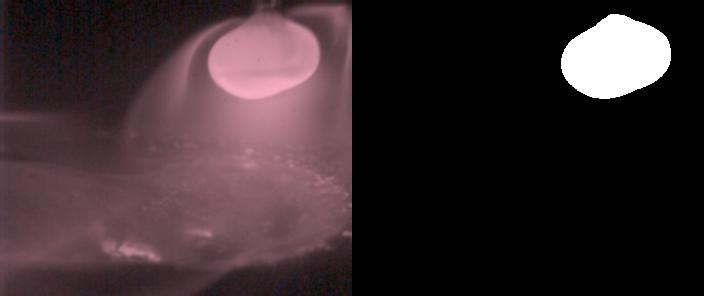
\includegraphics[width=\linewidth]{Images/Results/glob_pred_0.jpg}
    \caption{}

  \end{subfigure}
\hfill
  \begin{subfigure}[b]{0.45\textwidth}
    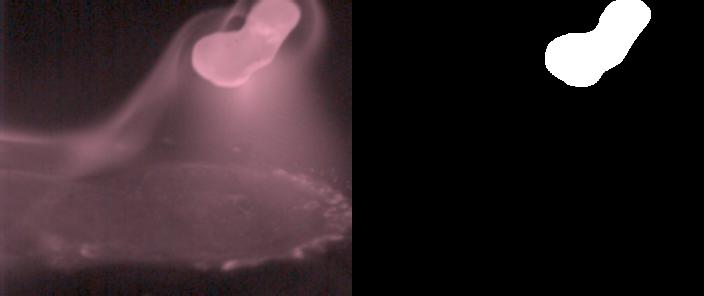
\includegraphics[width=\linewidth]{Images/Results/glob_pred_3870.jpg}
    \caption{}

  \end{subfigure}
  \begin{subfigure}[b]{0.45\textwidth}
    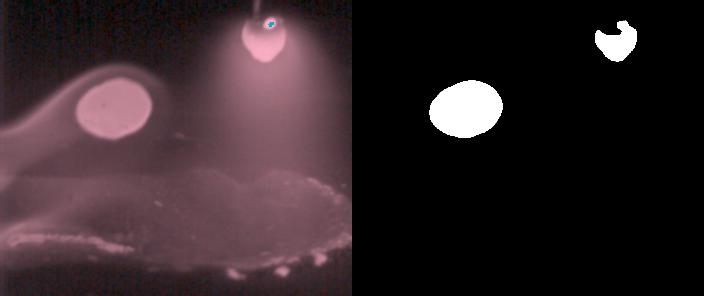
\includegraphics[width=\linewidth]{Images/Results/glob_pred_4817.jpg}
    \caption{}

  \end{subfigure}
    \caption[Globular transfer mode predictions]{Globular transfer mode predictions.}
    \label{fig:glob_pred_samples}
\end{figure}

\begin{figure}
\centering
  \begin{subfigure}[b]{0.45\textwidth}
    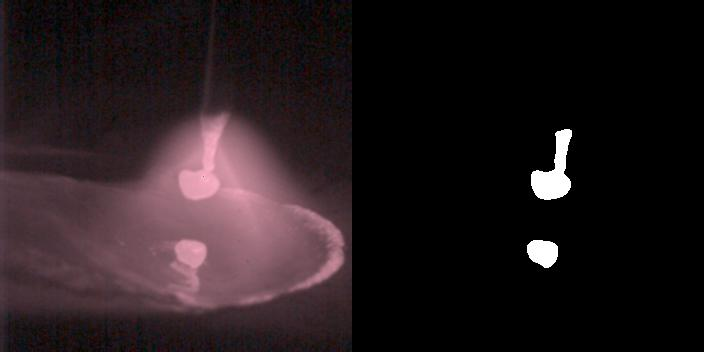
\includegraphics[width=\linewidth]{Images/Results/spray_pred_15.jpg}
    \caption{}

  \end{subfigure}
\hfill
  \begin{subfigure}[b]{0.45\textwidth}
    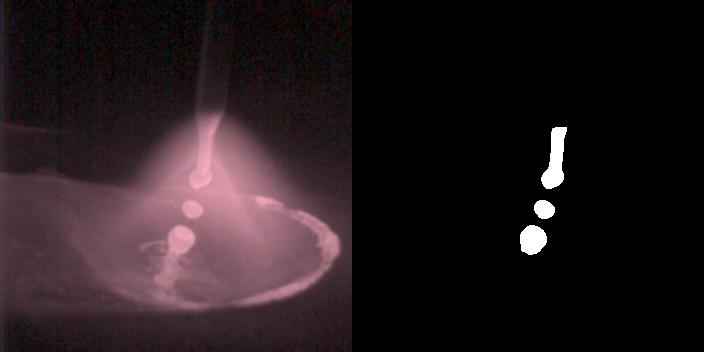
\includegraphics[width=\linewidth]{Images/Results/spray_pred_1937.jpg}
    \caption{}

  \end{subfigure}
  \begin{subfigure}[b]{0.45\textwidth}
    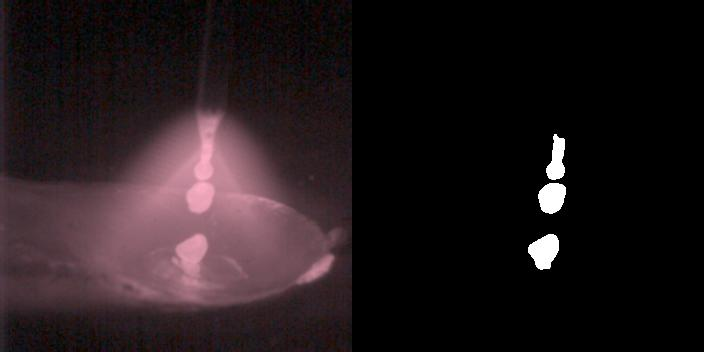
\includegraphics[width=\linewidth]{Images/Results/spray_pred_3269.jpg}
    \caption{}

  \end{subfigure}
    \caption[Spray transfer mode predictions]{Spray transfer mode predictions.}
    \label{fig:spray_pred_samples}
\end{figure}

Moreover, an important aspect of this work is that the labels were manually generated, so the results are subject to a human bias, specifically the selection of the boundary of the droplet because at a pixel level there is not an exact distinction between droplet and background and a gradient is seen between the brighter pixels of the droplet and the darker pixels of the background.

Hence, to make more evident where the network decides to make  the droplet-background division which is influenced by the labeling, figures \ref{fig:boundary_globular} and \ref{fig:boundary_spray} show the pixel values of a single horizontal strip, specifically the one that goes through the centroid of the droplet segmentation. There, one can see that there is a transition between droplet and background, and vertical lines show where the model cuts and makes the segmentation. The figures show that in the image there there is a steep transition between background and droplet, and the segmentation cuts around the middle of that transition. This results are also useful to assess the models' performance quantitatively since it is not possible to compute the loss function.

\begin{figure}
    \centering
    \import{Images/Results/boundary_globular/}{500.pgf}
    \caption[Predicted droplet boundary compared to original globular image]{Predicted droplet boundary compared to original globular image. A horizontal strip is taken along the droplet's centroid (dashed yellow line in (a) and (b)) and the pixel values along that line are shown in (c). In (b) the predicted mask which generates the red curve in (c) is shown.}
    \label{fig:boundary_globular}
\end{figure}

\begin{figure}
    \centering
    \import{Images/Results/boundary_spray/}{500.pgf}
    \caption[Predicted droplet boundary compared to original spray image]{Predicted droplet boundary compared to original spray image.}
    \label{fig:boundary_spray}
\end{figure}

\clearpage

\section{Post processing}
In this section the results after generating the segmentation maps are shown. These results consist in geometric and physical properties of the processes that help to understand them better. In Appendix \ref{appendix_postproc} there is a summary of the techniques used to obtain properties from the segmentation maps and signal processing in general.

\subsection{Centroids, velocity and acceleration}

The centroids of each frame are obtained using \texttt{opencv} which can identify contours in the segmented images and then compute the moments of each contour (see Appendix \ref{appendix_b1}). In images \ref{fig:globular_centroids} and \ref{fig:spray_centroids} some of the examples are shown. The results show that the centroids are accurately found in the segmentation maps and correspond to those in the original image. Moreover, it is possible to detect multiple contours within an image, so frames with more than one droplet have a separate centroid for each droplet.

In globular transfer, the growth process usually has only one droplet and when the droplet detaches, more droplets appear in the frame. This can be due to the main droplet splitting into two or more, or the network identifying the tip of the wire as another droplet or some portion of the weld pool which is too bright. The tip of the wire being identified as a droplet occurs because the melting of the wire is a continuous process, so when the droplet detaches, another droplet begins to form. Nevertheless, most of the time the initial state of the growth process does not have any segmented droplets, as shown in figure \ref{fig:globular_centroids_3}.

On the other hand, spray transfer has a faster growth and detachment of droplets since these are smaller than globular. This means that in most frames multiple droplets can be identified. The droplet forming in the wire is always segmented as a droplet and usually has an elongated shape because it is from where the droplets fall to the welding pool. The droplets that are falling have a more round shape compared to the one in the wire.

\begin{figure}
\centering
  \begin{subfigure}[b]{.95\textwidth}
    \import{Images/Results/centroid_samples/}{globular_0.pgf}
    \caption{}

  \end{subfigure}
\vfill
  \begin{subfigure}[b]{.95\textwidth}
    \import{Images/Results/centroid_samples/}{globular_790.pgf}
    \caption{}
  \end{subfigure}
  \vfill
 \begin{subfigure}[b]{.95\textwidth}
    \import{Images/Results/centroid_samples/}{globular_2360.pgf}
    \caption{}
    \label{fig:globular_centroids_3}
  \end{subfigure}
    \caption[Globular transfer mode centroid predictions]{Globular transfer mode centroid predictions. Black dots are used for single droplet and red crosses when multiple droplets are in the frame.}
    \label{fig:globular_centroids}
\end{figure}

\begin{figure}
\centering
  \begin{subfigure}[b]{.95\textwidth}
    \import{Images/Results/centroid_samples/}{spray_0.pgf}
    \caption{}

  \end{subfigure}
\vfill
  \begin{subfigure}[b]{.95\textwidth}
    \import{Images/Results/centroid_samples/}{spray_42.pgf}
    \caption{}
  \end{subfigure}
  \vfill
 \begin{subfigure}[b]{.95\textwidth}
    \import{Images/Results/centroid_samples/}{spray_656.pgf}
    \caption{}
  \end{subfigure}
    \caption[Spray transfer mode centroid predictions]{Spray transfer mode centroid predictions.}
    \label{fig:spray_centroids}
\end{figure}


Furthermore, given the $x$ and $y$ coordinates at each point in time, it is possible to compute velocity and acceleration. Specifically, free flight centroid data is used to compute velocity and acceleration, that is the periods of time in which the droplet is detached from the wire and has not yet reached the weld pool. Calculations are not made throughout the whole video since the focus should be in each single droplet, as opposed to the stream of droplets which would cause discontinuities in velocity or area, obfuscating the analysis. Since position measurements can be noisy, $x$ and $y$ positions are interpolated using a polynomial. A cubic function is used for globular and a quadratic for spray. The difference in functions is because in spray, free flight trajectory consists in around 5-10 frames which is quite low. Then, velocity and acceleration can be obtained analytically by differentiating the position function in each coordinate.

The identification of the droplet in the frame is a problem that has to be addressed since multiple centroids can appear in one image. In order to track a specific droplet through time, a continuity criterion is used. An initial droplet is selected. Then, at each frame the next centroids are compared to the current centroid and the one with the minimum euclidean distance is chosen since it is expected that a droplet can only move within its vicinity from frame to frame.

\begin{figure}
\centering
  \begin{subfigure}[b]{.8\textwidth}
    \import{Images/Results/kinematic/}{globular_trajectory_34-72.pgf}
  \end{subfigure}
\vfill
  \begin{subfigure}[b]{.8\textwidth}
    \import{Images/Results/kinematic/}{globular_trajectory_289-342.pgf}
  \end{subfigure}
\caption[Trajectory, velocity and acceleration of a free flight globular droplet for multiple time windows]{Trajectory, velocity (black arrows) and acceleration (red arrows) of a free flight globular droplet for multiple time windows. Trajectory is interpolated using a third degree polynomial in the $x$ and $y$ coordinates.} 
\label{fig:vel_glob}
\end{figure}

\begin{figure}
\centering
    \ContinuedFloat
    \captionsetup{list=off,format=cont}
  \begin{subfigure}[b]{.8\textwidth}
    \import{Images/Results/kinematic/}{globular_trajectory_1439-1502.pgf}
  \end{subfigure}
\vfill
  \begin{subfigure}[b]{.8\textwidth}
    \import{Images/Results/kinematic/}{globular_trajectory_2279-2341.pgf}
  \end{subfigure}
\caption{Trajectory, velocity and acceleration of a free flight globular droplet for multiple time windows.} 
\end{figure}

\begin{figure}
\centering
  \begin{subfigure}[b]{.8\textwidth}
    \import{Images/Results/kinematic/}{spray_trajectory_6-15.pgf}
  \end{subfigure}
\vfill
  \begin{subfigure}[b]{.8\textwidth}
    \import{Images/Results/kinematic/}{spray_trajectory_26-32.pgf}
  \end{subfigure}
\caption[Trajectory, velocity and acceleration of a free flight spray droplet for multiple time windows]{Trajectory, velocity (black arrows) and acceleration (red arrows) of a free flight spray droplet for multiple time windows. Trajectory is interpolated using a second degree polynomial in the $x$ and $y$ coordinates.} 
\label{fig:vel_spray}
\end{figure}

\begin{figure}
\centering
    \ContinuedFloat
    \captionsetup{list=off,format=cont}
  \begin{subfigure}[b]{.8\textwidth}
    \import{Images/Results/kinematic/}{spray_trajectory_49-56.pgf}
  \end{subfigure}
\vfill
  \begin{subfigure}[b]{.8\textwidth}
    \import{Images/Results/kinematic/}{spray_trajectory_59-67.pgf}
  \end{subfigure}
\caption{Trajectory, velocity and acceleration of a free flight spray droplet for multiple time windows.} 
\end{figure}

\begin{table}
\centering
\caption[Globular statistical features of velocity in each component for multiple free flight time windows]{Globular statistical features of velocity in each component for multiple free flight time windows.}
\label{tab:vel_glob}
\begin{tabular}{|c|cccccc|}
\hline
\multirow{2}{*}{Frames} & \multicolumn{2}{c}{\begin{tabular}[c]{@{}c@{}}Min\\ $[cm/s]$\end{tabular}} & \multicolumn{2}{c}{\begin{tabular}[c]{@{}c@{}}Max\\ $[cm/s]$\end{tabular}} & \multicolumn{2}{c|}{\begin{tabular}[c]{@{}c@{}}Mean $\pm$ Std. dev.\\ $[cm/s]$\end{tabular}} \\
 & $v_x$ & $v_y$ & $v_x$ & $v_y$ & $v_x$ & $v_y$ \\ \hline
$34-72$ & $-34.0$ & $13.8$ & $-19.1$ & $31.5$ & $-23.2\pm 3.9$ & $23.6\pm 5.1$ \\
$289-342$ & $-25.7$ & $6.1$ & $-21.0$ & $32.3$ & $-23.2\pm 1.3$ & $21.1\pm 7.6$ \\
$1429-1502$ & $-11.2$ & $14.6$ & $-7.4$ & $37.7$ & $-8.5\pm 1.0$ & $25.6\pm 6.7$ \\
$2279-2341$ & $-17.4$ & $16.3$ & $-12.3$ & $43.9$ & $-14.0\pm 1.5$ & $30.9\pm 7.9$ \\ \hline
\end{tabular}
\end{table}

\begin{table}
\centering
\caption[Globular statistical features of the norm of the velocity for multiple free flight time windows]{Globular statistical features of the norm of the velocity for multiple free flight time windows.}
\label{tab:vel_norm_glob}
\begin{tabular}{|c|ccc|}
\hline
\multicolumn{1}{|c|}{\multirow{2}{*}{Frames}} & \multicolumn{3}{c|}{$||\vec{v}||$} \\ \cline{2-4} 
\multicolumn{1}{|c|}{} & \multicolumn{1}{c}{\begin{tabular}[c]{@{}c@{}}Min\\ $[cm/s]$\end{tabular}} & \multicolumn{1}{c}{\begin{tabular}[c]{@{}c@{}}Max\\ $[cm/s]$\end{tabular}} & \multicolumn{1}{c|}{\begin{tabular}[c]{@{}c@{}}Mean $\pm$ Std. dev.\\ $[cm/s]$\end{tabular}} \\ \hline
$34-72$ & $28.3$ & $46.4$ & $33.4\pm 5.2$ \\
$289-342$ & $21.8$ & $41.3$ & $31.7\pm 5.9$ \\
$1429-1502$ & $17.8$ & $39.4$ & $27.1\pm 6.4$ \\
$2279-2341$ & $13.2$ & $18.3$ & $14.6\pm 1.4$ \\ \hline
\end{tabular}
\end{table}

\begin{table}
\centering
\caption[Globular statistical features of acceleration in each component for multiple free flight time windows]{Globular statistical features of acceleration for each component for multiple free flight time windows.}
\label{tab:acc_glob}
\begin{tabular}{|c|cccccc|}
\hline
\multirow{2}{*}{Frames} & \multicolumn{2}{c}{\begin{tabular}[c]{@{}c@{}}Min\\ $[m/s^2]$\end{tabular}} & \multicolumn{2}{c}{\begin{tabular}[c]{@{}c@{}}Max\\ $[m/s^2]$\end{tabular}} & \multicolumn{2}{c|}{\begin{tabular}[c]{@{}c@{}}Mean $\pm$ Std. dev.\\ $[m/s^2]$\end{tabular}} \\
 & $a_x$ & $a_y$ & $a_x$ & $a_y$ & $a_x$ & $a_y$ \\ \hline
$34-72$ & $-42.8$ & $9.5$ & $32.8$ & $19.2$ & $-4.9\pm 22.07$ & $14.3\pm 2.8$ \\
$289-342$ & $-3.3$ & $8.5$ & $-2.1$ & $21.6$ & $-2.7\pm 0.3$ & $15.0\pm 3.7$ \\
$1429-1502$ & $-6.7$ & $9.5$ & $5.7$ & $12.9$ & $-0.4\pm 3.6$ & $11.2\pm 0.9$ \\
$2279-2341$ & $-10.1$ & $11.6$ & $10.1$ & $15.2$ & $~0\pm 5.9$ & $13.4\pm 1.0$ \\ \hline
\end{tabular}
\end{table}

\begin{table}
\centering
\caption[Globular statistical features of the norm of the acceleration for multiple free flight time windows]{Globular statistical features of the norm of the acceleration for multiple free flight time windows.}
\label{tab:acc_norm_glob}
\begin{tabular}{|c|ccc|}
\hline
\multicolumn{1}{|c|}{\multirow{2}{*}{Frames}} & \multicolumn{3}{c|}{$||\vec{a}||$} \\ \cline{2-4} 
\multicolumn{1}{|c|}{} & \multicolumn{1}{c}{\begin{tabular}[c]{@{}c@{}}Min\\ $[m/s^2]$\end{tabular}} & \multicolumn{1}{c}{\begin{tabular}[c]{@{}c@{}}Max\\ $[m/s^2]$\end{tabular}} & \multicolumn{1}{c|}{\begin{tabular}[c]{@{}c@{}}Mean $\pm$ Std. dev.\\ $[m/s^2]$\end{tabular}} \\ \hline
$34-72$ & $14.8$ & $43.8$ & $25.6\pm 8.4$ \\
$289-342$ & $9.2$ & $21.7$ & $15.3\pm 3.6$ \\
$1429-1502$ & $10.6$ & $14.5$ & $11.7\pm 1.1$ \\
$2279-2341$ & $13.2$ & $18.3$ & $14.6\pm 1.4$ \\ \hline
\end{tabular}
\end{table}

\begin{table}
\centering
\caption[Spray statistical features of velocity in each component for multiple free flight time windows]{Spray statistical features of velocity in each component for multiple free flight time windows.}
\label{tab:vel_spray}
\begin{tabular}{|c|cccccc|}
\hline
\multirow{2}{*}{Frames} &
  \multicolumn{2}{c}{\begin{tabular}[c]{@{}c@{}}Min\\ $[cm/s]$\end{tabular}} &
  \multicolumn{2}{c}{\begin{tabular}[c]{@{}c@{}}Max\\ $[cm/s]$\end{tabular}} &
  \multicolumn{2}{c|}{\begin{tabular}[c]{@{}c@{}}Mean $\pm$ Std. dev.\\ $[cm/s]$\end{tabular}} \\
        & $v_x$   & $v_y$   & $v_x$   & $v_y$   & $v_x$          & $v_y$          \\ \hline
$6-15$  & $-20.8$ & $73.8$  & $-18.6$ & $81.5$  & $-19.7\pm 0.6$ & $77.6\pm 2.2$  \\
$26-32$ & $-23.7$ & $94.0$  & $-22.4$ & $100.2$ & $-23.1\pm 0.3$ & $97.1\pm 1.7$  \\
$49-56$ & $2.2$   & $102.3$ & $9.51$  & $111.5$ & $5.8\pm 2.1$   & $106.9\pm 2.6$ \\
$59-67$ & $-11.3$ & $123.5$ & $-5.3$  & $128.4$ & $-8.3\pm 1.7$  & $126.0\pm 1.4$ \\ \hline
\end{tabular}
\end{table}


\begin{table}
\centering
\caption[Spray statistical features of the norm of the velocity for multiple free flight time windows]{Spray statistical features of the norm of the velocity for multiple free flight time windows.}
\label{tab:vel_norm_spray}
\begin{tabular}{|c|ccc|}
\hline
\multirow{2}{*}{Frames} & \multicolumn{3}{c|}{$||\vec{v}||$} \\ \cline{2-4} 
 &
  \begin{tabular}[c]{@{}c@{}}Min\\ $[cm/s]$\end{tabular} &
  \begin{tabular}[c]{@{}c@{}}Max\\ $[cm/s]$\end{tabular} &
  \begin{tabular}[c]{@{}c@{}}Mean $\pm$ Std. dev.\\ $[cm/s]$\end{tabular} \\ \hline
$6-15$                  & $76.7$  & $83.6$  & $80.1\pm 2.0$  \\
$26-32$                 & $97.0$  & $102.6$ & $99.8\pm 1.6$  \\
$49-56$                 & $102.4$ & $111.9$ & $107.1\pm 2.7$ \\
$59-67$                 & $124.1$ & $128.5$ & $126.3\pm 1.2$ \\ \hline
\end{tabular}
\end{table}

\begin{table}
\centering
\caption[Spray features of acceleration for multiple free flight time windows]{Spray features of acceleration for multiple free flight time windows (acceleration is constant since trajectory is assumed to be a second degree polynomial).}
\label{tab:acc_spray}
\begin{tabular}{|c|ccc|}
\hline
Frames  & $a_x$   & $a_y$   & $||\vec{a}||$ \\ \hline
$6-15$  & $8.3$   & $29.0$  & $30.2$        \\
$26-32$ & $-7.9$  & $-36.7$ & $37.6$        \\
$49-56$ & $-36.4$ & $-45.8$ & $58.5$        \\
$59-67$ & $-25.9$ & $-20.8$ & $33.2$        \\ \hline
\end{tabular}
\end{table}

The trajectory, velocity and acceleration of different free flight droplet motion can be seen in figures \ref{fig:vel_glob} and \ref{fig:vel_spray} for globular and spray respectively. Also, statistical features for velocity and acceleration are shown in tables \ref{tab:vel_glob} through \ref{tab:acc_spray}. Notice that the axes correspond to the $x$ and $y$ position of the centroid in the image converted to distance and the origin is on the top left. 

Displacement in $y$ is more or less fixed since the droplet will always land at about the same height while $x$ displacement ranges from $1\:mm$ up to $4\;mm$ in globular and less than $1\;mm$ in spray. A smaller $x$ displacement is also seen in the velocity having a larger $y$ component, hence landing faster as seen in spray trajectories (fig. \ref{fig:vel_spray}). Furthermore, velocity is around $30\;cm/s$ in globular while spray is much more, reaching around $100\;cm/s$. Also, acceleration is around $15\;m/s^2$ for globular and $40\:m/s^2$ in spray. As expected, spray transfer tends to be faster than globular since cycles are much shorter. It is worth noting that the spray acceleration does have a less intuitive pattern pointing upwards in general which may be due to the small sample of the trajectory points because interpolating values and then differentiating can induce more error.

In comparison, in the work of \textit{Weglowski} \cite{vel}, accelerations between $90-140 \;m/s^2$ are obtained for varying experimental setups. Moreover, in the work of\textit{Hu} \cite{vel2} acceleration ranges within $20-50\;m/s^2$. Similar values are found in \textit{Ray} \cite{Ray}. Acceleration values found here are within the order of magnitude of previous work, specially when compared to \textit{Hu} and \textit{Ray} \cite{vel2,Ray}. Differences may be due to different experimental setups, but also because of the inherent error when interpolating and differentiating twice for acceleration. In the case of velocity, ranges of $50-100\;cm/s$ and $20-50\;cm/s$ are found \cite{vel,vel2} which mostly coincide with those calculated in this work.

Although these computations should be accurate based on the segmentation accuracy and subsequent centroid position, it is worth noting that higher resolution in time (sampling frequency) would get better results because centroid displacements can be too fast and rough trajectories are seen, this phenomenon can be observed in the graphs of figures \ref{fig:vel_glob} and specially \ref{fig:vel_spray} in which the scarcity of data points for trajectory is evident.

\subsection{Area and detachment rate}

The contours found in each image can also be used to compute the area of a droplet\footnote{Perimeter and volume are also computed and show similar trends.}. Since the segmentation maps are binary, this can be done simply by summing all of the pixel intensities inside a given contour. Then, using the relationship in \eqref{eq:px_to_mm}, it is possible to estimate the area in $mm^2$ as shown in figures \ref{fig:globular_areas} and \ref{fig:spray_areas}\footnote{Not all the frames are displayed so the plot does not get cluttered. The full graph can be seen in video format in the GitHub project.}.

The globular case shows a pattern where there is a growing phase in which only one droplet is detected (black dots), then the area drops suddenly and the number of droplets detected is more than one (red crosses). Later, the network detects no droplets in the frame for a brief time (blue dots) and then the cycle is repeated.

Since the value of the area is an indicator of when the droplet detaches from the wire, it would be useful to detect when this is happening. This is done by smoothing the signal using a \textit{hanning} window and convolving it with the original signal which effectively works as a weighted average. Notice that since the area can have multiple values for a given frame, the sum of these values is used instead. In this way, the smoothed signal is easier to process simply by finding its peaks, which is carried out using \texttt{scipy}'s \texttt{find\_peaks} function which allows to set a variety of parameters such as height, prominence and width of peaks\footnote{Notice that \texttt{scipy} finds maximum peaks and in this case the opposite is needed, so in practice the negative value of the signal is used.}. As seen in figure \ref{fig:globular_areas}, the smoothed curve's (green curve) minimum peaks (vertical dashed lines) coincide with the detachment of droplets accurately. In this way it is possible to count the number of droplets over time as well as the point in time when that occurs. Specifically, the number of globular droplet detachments observed is 25 while the detected is 24.

\begin{figure}
  \begin{subfigure}[b]{\textwidth}
    %% Creator: Matplotlib, PGF backend
%%
%% To include the figure in your LaTeX document, write
%%   \input{<filename>.pgf}
%%
%% Make sure the required packages are loaded in your preamble
%%   \usepackage{pgf}
%%
%% and, on pdftex
%%   \usepackage[utf8]{inputenc}\DeclareUnicodeCharacter{2212}{-}
%%
%% or, on luatex and xetex
%%   \usepackage{unicode-math}
%%
%% Figures using additional raster images can only be included by \input if
%% they are in the same directory as the main LaTeX file. For loading figures
%% from other directories you can use the `import` package
%%   \usepackage{import}
%%
%% and then include the figures with
%%   \import{<path to file>}{<filename>.pgf}
%%
%% Matplotlib used the following preamble
%%
\begingroup%
\makeatletter%
\begin{pgfpicture}%
\pgfpathrectangle{\pgfpointorigin}{\pgfqpoint{6.531496in}{3.265748in}}%
\pgfusepath{use as bounding box, clip}%
\begin{pgfscope}%
\pgfsetbuttcap%
\pgfsetmiterjoin%
\definecolor{currentfill}{rgb}{1.000000,1.000000,1.000000}%
\pgfsetfillcolor{currentfill}%
\pgfsetlinewidth{0.000000pt}%
\definecolor{currentstroke}{rgb}{1.000000,1.000000,1.000000}%
\pgfsetstrokecolor{currentstroke}%
\pgfsetdash{}{0pt}%
\pgfpathmoveto{\pgfqpoint{0.000000in}{0.000000in}}%
\pgfpathlineto{\pgfqpoint{6.531496in}{0.000000in}}%
\pgfpathlineto{\pgfqpoint{6.531496in}{3.265748in}}%
\pgfpathlineto{\pgfqpoint{0.000000in}{3.265748in}}%
\pgfpathclose%
\pgfusepath{fill}%
\end{pgfscope}%
\begin{pgfscope}%
\pgfsetbuttcap%
\pgfsetmiterjoin%
\definecolor{currentfill}{rgb}{0.917647,0.917647,0.949020}%
\pgfsetfillcolor{currentfill}%
\pgfsetlinewidth{0.000000pt}%
\definecolor{currentstroke}{rgb}{0.000000,0.000000,0.000000}%
\pgfsetstrokecolor{currentstroke}%
\pgfsetstrokeopacity{0.000000}%
\pgfsetdash{}{0pt}%
\pgfpathmoveto{\pgfqpoint{0.819958in}{0.650833in}}%
\pgfpathlineto{\pgfqpoint{6.351496in}{0.650833in}}%
\pgfpathlineto{\pgfqpoint{6.351496in}{3.085748in}}%
\pgfpathlineto{\pgfqpoint{0.819958in}{3.085748in}}%
\pgfpathclose%
\pgfusepath{fill}%
\end{pgfscope}%
\begin{pgfscope}%
\pgfpathrectangle{\pgfqpoint{0.819958in}{0.650833in}}{\pgfqpoint{5.531539in}{2.434915in}}%
\pgfusepath{clip}%
\pgfsetroundcap%
\pgfsetroundjoin%
\pgfsetlinewidth{1.003750pt}%
\definecolor{currentstroke}{rgb}{1.000000,1.000000,1.000000}%
\pgfsetstrokecolor{currentstroke}%
\pgfsetdash{}{0pt}%
\pgfpathmoveto{\pgfqpoint{1.071391in}{0.650833in}}%
\pgfpathlineto{\pgfqpoint{1.071391in}{3.085748in}}%
\pgfusepath{stroke}%
\end{pgfscope}%
\begin{pgfscope}%
\definecolor{textcolor}{rgb}{0.150000,0.150000,0.150000}%
\pgfsetstrokecolor{textcolor}%
\pgfsetfillcolor{textcolor}%
\pgftext[x=1.071391in,y=0.518888in,,top]{\color{textcolor}\rmfamily\fontsize{11.000000}{13.200000}\selectfont \(\displaystyle {0}\)}%
\end{pgfscope}%
\begin{pgfscope}%
\pgfpathrectangle{\pgfqpoint{0.819958in}{0.650833in}}{\pgfqpoint{5.531539in}{2.434915in}}%
\pgfusepath{clip}%
\pgfsetroundcap%
\pgfsetroundjoin%
\pgfsetlinewidth{1.003750pt}%
\definecolor{currentstroke}{rgb}{1.000000,1.000000,1.000000}%
\pgfsetstrokecolor{currentstroke}%
\pgfsetdash{}{0pt}%
\pgfpathmoveto{\pgfqpoint{2.078132in}{0.650833in}}%
\pgfpathlineto{\pgfqpoint{2.078132in}{3.085748in}}%
\pgfusepath{stroke}%
\end{pgfscope}%
\begin{pgfscope}%
\definecolor{textcolor}{rgb}{0.150000,0.150000,0.150000}%
\pgfsetstrokecolor{textcolor}%
\pgfsetfillcolor{textcolor}%
\pgftext[x=2.078132in,y=0.518888in,,top]{\color{textcolor}\rmfamily\fontsize{11.000000}{13.200000}\selectfont \(\displaystyle {200}\)}%
\end{pgfscope}%
\begin{pgfscope}%
\pgfpathrectangle{\pgfqpoint{0.819958in}{0.650833in}}{\pgfqpoint{5.531539in}{2.434915in}}%
\pgfusepath{clip}%
\pgfsetroundcap%
\pgfsetroundjoin%
\pgfsetlinewidth{1.003750pt}%
\definecolor{currentstroke}{rgb}{1.000000,1.000000,1.000000}%
\pgfsetstrokecolor{currentstroke}%
\pgfsetdash{}{0pt}%
\pgfpathmoveto{\pgfqpoint{3.084873in}{0.650833in}}%
\pgfpathlineto{\pgfqpoint{3.084873in}{3.085748in}}%
\pgfusepath{stroke}%
\end{pgfscope}%
\begin{pgfscope}%
\definecolor{textcolor}{rgb}{0.150000,0.150000,0.150000}%
\pgfsetstrokecolor{textcolor}%
\pgfsetfillcolor{textcolor}%
\pgftext[x=3.084873in,y=0.518888in,,top]{\color{textcolor}\rmfamily\fontsize{11.000000}{13.200000}\selectfont \(\displaystyle {400}\)}%
\end{pgfscope}%
\begin{pgfscope}%
\pgfpathrectangle{\pgfqpoint{0.819958in}{0.650833in}}{\pgfqpoint{5.531539in}{2.434915in}}%
\pgfusepath{clip}%
\pgfsetroundcap%
\pgfsetroundjoin%
\pgfsetlinewidth{1.003750pt}%
\definecolor{currentstroke}{rgb}{1.000000,1.000000,1.000000}%
\pgfsetstrokecolor{currentstroke}%
\pgfsetdash{}{0pt}%
\pgfpathmoveto{\pgfqpoint{4.091614in}{0.650833in}}%
\pgfpathlineto{\pgfqpoint{4.091614in}{3.085748in}}%
\pgfusepath{stroke}%
\end{pgfscope}%
\begin{pgfscope}%
\definecolor{textcolor}{rgb}{0.150000,0.150000,0.150000}%
\pgfsetstrokecolor{textcolor}%
\pgfsetfillcolor{textcolor}%
\pgftext[x=4.091614in,y=0.518888in,,top]{\color{textcolor}\rmfamily\fontsize{11.000000}{13.200000}\selectfont \(\displaystyle {600}\)}%
\end{pgfscope}%
\begin{pgfscope}%
\pgfpathrectangle{\pgfqpoint{0.819958in}{0.650833in}}{\pgfqpoint{5.531539in}{2.434915in}}%
\pgfusepath{clip}%
\pgfsetroundcap%
\pgfsetroundjoin%
\pgfsetlinewidth{1.003750pt}%
\definecolor{currentstroke}{rgb}{1.000000,1.000000,1.000000}%
\pgfsetstrokecolor{currentstroke}%
\pgfsetdash{}{0pt}%
\pgfpathmoveto{\pgfqpoint{5.098355in}{0.650833in}}%
\pgfpathlineto{\pgfqpoint{5.098355in}{3.085748in}}%
\pgfusepath{stroke}%
\end{pgfscope}%
\begin{pgfscope}%
\definecolor{textcolor}{rgb}{0.150000,0.150000,0.150000}%
\pgfsetstrokecolor{textcolor}%
\pgfsetfillcolor{textcolor}%
\pgftext[x=5.098355in,y=0.518888in,,top]{\color{textcolor}\rmfamily\fontsize{11.000000}{13.200000}\selectfont \(\displaystyle {800}\)}%
\end{pgfscope}%
\begin{pgfscope}%
\pgfpathrectangle{\pgfqpoint{0.819958in}{0.650833in}}{\pgfqpoint{5.531539in}{2.434915in}}%
\pgfusepath{clip}%
\pgfsetroundcap%
\pgfsetroundjoin%
\pgfsetlinewidth{1.003750pt}%
\definecolor{currentstroke}{rgb}{1.000000,1.000000,1.000000}%
\pgfsetstrokecolor{currentstroke}%
\pgfsetdash{}{0pt}%
\pgfpathmoveto{\pgfqpoint{6.105096in}{0.650833in}}%
\pgfpathlineto{\pgfqpoint{6.105096in}{3.085748in}}%
\pgfusepath{stroke}%
\end{pgfscope}%
\begin{pgfscope}%
\definecolor{textcolor}{rgb}{0.150000,0.150000,0.150000}%
\pgfsetstrokecolor{textcolor}%
\pgfsetfillcolor{textcolor}%
\pgftext[x=6.105096in,y=0.518888in,,top]{\color{textcolor}\rmfamily\fontsize{11.000000}{13.200000}\selectfont \(\displaystyle {1000}\)}%
\end{pgfscope}%
\begin{pgfscope}%
\definecolor{textcolor}{rgb}{0.150000,0.150000,0.150000}%
\pgfsetstrokecolor{textcolor}%
\pgfsetfillcolor{textcolor}%
\pgftext[x=3.585727in,y=0.328147in,,top]{\color{textcolor}\rmfamily\fontsize{12.000000}{14.400000}\selectfont Frame}%
\end{pgfscope}%
\begin{pgfscope}%
\pgfpathrectangle{\pgfqpoint{0.819958in}{0.650833in}}{\pgfqpoint{5.531539in}{2.434915in}}%
\pgfusepath{clip}%
\pgfsetroundcap%
\pgfsetroundjoin%
\pgfsetlinewidth{1.003750pt}%
\definecolor{currentstroke}{rgb}{1.000000,1.000000,1.000000}%
\pgfsetstrokecolor{currentstroke}%
\pgfsetdash{}{0pt}%
\pgfpathmoveto{\pgfqpoint{0.819958in}{0.665736in}}%
\pgfpathlineto{\pgfqpoint{6.351496in}{0.665736in}}%
\pgfusepath{stroke}%
\end{pgfscope}%
\begin{pgfscope}%
\definecolor{textcolor}{rgb}{0.150000,0.150000,0.150000}%
\pgfsetstrokecolor{textcolor}%
\pgfsetfillcolor{textcolor}%
\pgftext[x=0.493684in, y=0.612930in, left, base]{\color{textcolor}\rmfamily\fontsize{11.000000}{13.200000}\selectfont \(\displaystyle {0.0}\)}%
\end{pgfscope}%
\begin{pgfscope}%
\pgfpathrectangle{\pgfqpoint{0.819958in}{0.650833in}}{\pgfqpoint{5.531539in}{2.434915in}}%
\pgfusepath{clip}%
\pgfsetroundcap%
\pgfsetroundjoin%
\pgfsetlinewidth{1.003750pt}%
\definecolor{currentstroke}{rgb}{1.000000,1.000000,1.000000}%
\pgfsetstrokecolor{currentstroke}%
\pgfsetdash{}{0pt}%
\pgfpathmoveto{\pgfqpoint{0.819958in}{1.038327in}}%
\pgfpathlineto{\pgfqpoint{6.351496in}{1.038327in}}%
\pgfusepath{stroke}%
\end{pgfscope}%
\begin{pgfscope}%
\definecolor{textcolor}{rgb}{0.150000,0.150000,0.150000}%
\pgfsetstrokecolor{textcolor}%
\pgfsetfillcolor{textcolor}%
\pgftext[x=0.493684in, y=0.985521in, left, base]{\color{textcolor}\rmfamily\fontsize{11.000000}{13.200000}\selectfont \(\displaystyle {2.5}\)}%
\end{pgfscope}%
\begin{pgfscope}%
\pgfpathrectangle{\pgfqpoint{0.819958in}{0.650833in}}{\pgfqpoint{5.531539in}{2.434915in}}%
\pgfusepath{clip}%
\pgfsetroundcap%
\pgfsetroundjoin%
\pgfsetlinewidth{1.003750pt}%
\definecolor{currentstroke}{rgb}{1.000000,1.000000,1.000000}%
\pgfsetstrokecolor{currentstroke}%
\pgfsetdash{}{0pt}%
\pgfpathmoveto{\pgfqpoint{0.819958in}{1.410919in}}%
\pgfpathlineto{\pgfqpoint{6.351496in}{1.410919in}}%
\pgfusepath{stroke}%
\end{pgfscope}%
\begin{pgfscope}%
\definecolor{textcolor}{rgb}{0.150000,0.150000,0.150000}%
\pgfsetstrokecolor{textcolor}%
\pgfsetfillcolor{textcolor}%
\pgftext[x=0.493684in, y=1.358112in, left, base]{\color{textcolor}\rmfamily\fontsize{11.000000}{13.200000}\selectfont \(\displaystyle {5.0}\)}%
\end{pgfscope}%
\begin{pgfscope}%
\pgfpathrectangle{\pgfqpoint{0.819958in}{0.650833in}}{\pgfqpoint{5.531539in}{2.434915in}}%
\pgfusepath{clip}%
\pgfsetroundcap%
\pgfsetroundjoin%
\pgfsetlinewidth{1.003750pt}%
\definecolor{currentstroke}{rgb}{1.000000,1.000000,1.000000}%
\pgfsetstrokecolor{currentstroke}%
\pgfsetdash{}{0pt}%
\pgfpathmoveto{\pgfqpoint{0.819958in}{1.783510in}}%
\pgfpathlineto{\pgfqpoint{6.351496in}{1.783510in}}%
\pgfusepath{stroke}%
\end{pgfscope}%
\begin{pgfscope}%
\definecolor{textcolor}{rgb}{0.150000,0.150000,0.150000}%
\pgfsetstrokecolor{textcolor}%
\pgfsetfillcolor{textcolor}%
\pgftext[x=0.493684in, y=1.730703in, left, base]{\color{textcolor}\rmfamily\fontsize{11.000000}{13.200000}\selectfont \(\displaystyle {7.5}\)}%
\end{pgfscope}%
\begin{pgfscope}%
\pgfpathrectangle{\pgfqpoint{0.819958in}{0.650833in}}{\pgfqpoint{5.531539in}{2.434915in}}%
\pgfusepath{clip}%
\pgfsetroundcap%
\pgfsetroundjoin%
\pgfsetlinewidth{1.003750pt}%
\definecolor{currentstroke}{rgb}{1.000000,1.000000,1.000000}%
\pgfsetstrokecolor{currentstroke}%
\pgfsetdash{}{0pt}%
\pgfpathmoveto{\pgfqpoint{0.819958in}{2.156101in}}%
\pgfpathlineto{\pgfqpoint{6.351496in}{2.156101in}}%
\pgfusepath{stroke}%
\end{pgfscope}%
\begin{pgfscope}%
\definecolor{textcolor}{rgb}{0.150000,0.150000,0.150000}%
\pgfsetstrokecolor{textcolor}%
\pgfsetfillcolor{textcolor}%
\pgftext[x=0.417643in, y=2.103294in, left, base]{\color{textcolor}\rmfamily\fontsize{11.000000}{13.200000}\selectfont \(\displaystyle {10.0}\)}%
\end{pgfscope}%
\begin{pgfscope}%
\pgfpathrectangle{\pgfqpoint{0.819958in}{0.650833in}}{\pgfqpoint{5.531539in}{2.434915in}}%
\pgfusepath{clip}%
\pgfsetroundcap%
\pgfsetroundjoin%
\pgfsetlinewidth{1.003750pt}%
\definecolor{currentstroke}{rgb}{1.000000,1.000000,1.000000}%
\pgfsetstrokecolor{currentstroke}%
\pgfsetdash{}{0pt}%
\pgfpathmoveto{\pgfqpoint{0.819958in}{2.528692in}}%
\pgfpathlineto{\pgfqpoint{6.351496in}{2.528692in}}%
\pgfusepath{stroke}%
\end{pgfscope}%
\begin{pgfscope}%
\definecolor{textcolor}{rgb}{0.150000,0.150000,0.150000}%
\pgfsetstrokecolor{textcolor}%
\pgfsetfillcolor{textcolor}%
\pgftext[x=0.417643in, y=2.475885in, left, base]{\color{textcolor}\rmfamily\fontsize{11.000000}{13.200000}\selectfont \(\displaystyle {12.5}\)}%
\end{pgfscope}%
\begin{pgfscope}%
\pgfpathrectangle{\pgfqpoint{0.819958in}{0.650833in}}{\pgfqpoint{5.531539in}{2.434915in}}%
\pgfusepath{clip}%
\pgfsetroundcap%
\pgfsetroundjoin%
\pgfsetlinewidth{1.003750pt}%
\definecolor{currentstroke}{rgb}{1.000000,1.000000,1.000000}%
\pgfsetstrokecolor{currentstroke}%
\pgfsetdash{}{0pt}%
\pgfpathmoveto{\pgfqpoint{0.819958in}{2.901283in}}%
\pgfpathlineto{\pgfqpoint{6.351496in}{2.901283in}}%
\pgfusepath{stroke}%
\end{pgfscope}%
\begin{pgfscope}%
\definecolor{textcolor}{rgb}{0.150000,0.150000,0.150000}%
\pgfsetstrokecolor{textcolor}%
\pgfsetfillcolor{textcolor}%
\pgftext[x=0.417643in, y=2.848476in, left, base]{\color{textcolor}\rmfamily\fontsize{11.000000}{13.200000}\selectfont \(\displaystyle {15.0}\)}%
\end{pgfscope}%
\begin{pgfscope}%
\definecolor{textcolor}{rgb}{0.150000,0.150000,0.150000}%
\pgfsetstrokecolor{textcolor}%
\pgfsetfillcolor{textcolor}%
\pgftext[x=0.362087in,y=1.868290in,,bottom,rotate=90.000000]{\color{textcolor}\rmfamily\fontsize{12.000000}{14.400000}\selectfont Area [\(\displaystyle mm^2\)]}%
\end{pgfscope}%
\begin{pgfscope}%
\pgfpathrectangle{\pgfqpoint{0.819958in}{0.650833in}}{\pgfqpoint{5.531539in}{2.434915in}}%
\pgfusepath{clip}%
\pgfsetbuttcap%
\pgfsetroundjoin%
\definecolor{currentfill}{rgb}{0.298039,0.447059,0.690196}%
\pgfsetfillcolor{currentfill}%
\pgfsetlinewidth{1.003750pt}%
\definecolor{currentstroke}{rgb}{0.298039,0.447059,0.690196}%
\pgfsetstrokecolor{currentstroke}%
\pgfsetdash{}{0pt}%
\pgfsys@defobject{currentmarker}{\pgfqpoint{-0.024056in}{-0.024056in}}{\pgfqpoint{0.024056in}{0.024056in}}{%
\pgfpathmoveto{\pgfqpoint{0.000000in}{-0.024056in}}%
\pgfpathcurveto{\pgfqpoint{0.006380in}{-0.024056in}}{\pgfqpoint{0.012499in}{-0.021522in}}{\pgfqpoint{0.017010in}{-0.017010in}}%
\pgfpathcurveto{\pgfqpoint{0.021522in}{-0.012499in}}{\pgfqpoint{0.024056in}{-0.006380in}}{\pgfqpoint{0.024056in}{0.000000in}}%
\pgfpathcurveto{\pgfqpoint{0.024056in}{0.006380in}}{\pgfqpoint{0.021522in}{0.012499in}}{\pgfqpoint{0.017010in}{0.017010in}}%
\pgfpathcurveto{\pgfqpoint{0.012499in}{0.021522in}}{\pgfqpoint{0.006380in}{0.024056in}}{\pgfqpoint{0.000000in}{0.024056in}}%
\pgfpathcurveto{\pgfqpoint{-0.006380in}{0.024056in}}{\pgfqpoint{-0.012499in}{0.021522in}}{\pgfqpoint{-0.017010in}{0.017010in}}%
\pgfpathcurveto{\pgfqpoint{-0.021522in}{0.012499in}}{\pgfqpoint{-0.024056in}{0.006380in}}{\pgfqpoint{-0.024056in}{0.000000in}}%
\pgfpathcurveto{\pgfqpoint{-0.024056in}{-0.006380in}}{\pgfqpoint{-0.021522in}{-0.012499in}}{\pgfqpoint{-0.017010in}{-0.017010in}}%
\pgfpathcurveto{\pgfqpoint{-0.012499in}{-0.021522in}}{\pgfqpoint{-0.006380in}{-0.024056in}}{\pgfqpoint{0.000000in}{-0.024056in}}%
\pgfpathclose%
\pgfusepath{stroke,fill}%
}%
\begin{pgfscope}%
\pgfsys@transformshift{1.524425in}{0.665736in}%
\pgfsys@useobject{currentmarker}{}%
\end{pgfscope}%
\begin{pgfscope}%
\pgfsys@transformshift{1.534492in}{0.665736in}%
\pgfsys@useobject{currentmarker}{}%
\end{pgfscope}%
\begin{pgfscope}%
\pgfsys@transformshift{1.539526in}{0.665736in}%
\pgfsys@useobject{currentmarker}{}%
\end{pgfscope}%
\begin{pgfscope}%
\pgfsys@transformshift{1.544559in}{0.665736in}%
\pgfsys@useobject{currentmarker}{}%
\end{pgfscope}%
\begin{pgfscope}%
\pgfsys@transformshift{1.549593in}{0.665736in}%
\pgfsys@useobject{currentmarker}{}%
\end{pgfscope}%
\begin{pgfscope}%
\pgfsys@transformshift{1.554627in}{0.665736in}%
\pgfsys@useobject{currentmarker}{}%
\end{pgfscope}%
\begin{pgfscope}%
\pgfsys@transformshift{1.559661in}{0.665736in}%
\pgfsys@useobject{currentmarker}{}%
\end{pgfscope}%
\begin{pgfscope}%
\pgfsys@transformshift{1.564694in}{0.665736in}%
\pgfsys@useobject{currentmarker}{}%
\end{pgfscope}%
\begin{pgfscope}%
\pgfsys@transformshift{1.569728in}{0.665736in}%
\pgfsys@useobject{currentmarker}{}%
\end{pgfscope}%
\begin{pgfscope}%
\pgfsys@transformshift{1.574762in}{0.665736in}%
\pgfsys@useobject{currentmarker}{}%
\end{pgfscope}%
\begin{pgfscope}%
\pgfsys@transformshift{1.579795in}{0.665736in}%
\pgfsys@useobject{currentmarker}{}%
\end{pgfscope}%
\begin{pgfscope}%
\pgfsys@transformshift{1.584829in}{0.665736in}%
\pgfsys@useobject{currentmarker}{}%
\end{pgfscope}%
\begin{pgfscope}%
\pgfsys@transformshift{1.589863in}{0.665736in}%
\pgfsys@useobject{currentmarker}{}%
\end{pgfscope}%
\begin{pgfscope}%
\pgfsys@transformshift{1.599930in}{0.665736in}%
\pgfsys@useobject{currentmarker}{}%
\end{pgfscope}%
\begin{pgfscope}%
\pgfsys@transformshift{1.604964in}{0.665736in}%
\pgfsys@useobject{currentmarker}{}%
\end{pgfscope}%
\begin{pgfscope}%
\pgfsys@transformshift{1.609998in}{0.665736in}%
\pgfsys@useobject{currentmarker}{}%
\end{pgfscope}%
\begin{pgfscope}%
\pgfsys@transformshift{1.630132in}{0.665736in}%
\pgfsys@useobject{currentmarker}{}%
\end{pgfscope}%
\begin{pgfscope}%
\pgfsys@transformshift{1.635166in}{0.665736in}%
\pgfsys@useobject{currentmarker}{}%
\end{pgfscope}%
\begin{pgfscope}%
\pgfsys@transformshift{1.640200in}{0.665736in}%
\pgfsys@useobject{currentmarker}{}%
\end{pgfscope}%
\begin{pgfscope}%
\pgfsys@transformshift{1.645234in}{0.665736in}%
\pgfsys@useobject{currentmarker}{}%
\end{pgfscope}%
\begin{pgfscope}%
\pgfsys@transformshift{1.650267in}{0.665736in}%
\pgfsys@useobject{currentmarker}{}%
\end{pgfscope}%
\begin{pgfscope}%
\pgfsys@transformshift{1.660335in}{0.665736in}%
\pgfsys@useobject{currentmarker}{}%
\end{pgfscope}%
\begin{pgfscope}%
\pgfsys@transformshift{1.665368in}{0.665736in}%
\pgfsys@useobject{currentmarker}{}%
\end{pgfscope}%
\begin{pgfscope}%
\pgfsys@transformshift{2.848289in}{0.665736in}%
\pgfsys@useobject{currentmarker}{}%
\end{pgfscope}%
\begin{pgfscope}%
\pgfsys@transformshift{2.853323in}{0.665736in}%
\pgfsys@useobject{currentmarker}{}%
\end{pgfscope}%
\begin{pgfscope}%
\pgfsys@transformshift{2.858357in}{0.665736in}%
\pgfsys@useobject{currentmarker}{}%
\end{pgfscope}%
\begin{pgfscope}%
\pgfsys@transformshift{2.863390in}{0.665736in}%
\pgfsys@useobject{currentmarker}{}%
\end{pgfscope}%
\begin{pgfscope}%
\pgfsys@transformshift{2.868424in}{0.665736in}%
\pgfsys@useobject{currentmarker}{}%
\end{pgfscope}%
\begin{pgfscope}%
\pgfsys@transformshift{2.873458in}{0.665736in}%
\pgfsys@useobject{currentmarker}{}%
\end{pgfscope}%
\begin{pgfscope}%
\pgfsys@transformshift{2.878491in}{0.665736in}%
\pgfsys@useobject{currentmarker}{}%
\end{pgfscope}%
\begin{pgfscope}%
\pgfsys@transformshift{2.918761in}{0.665736in}%
\pgfsys@useobject{currentmarker}{}%
\end{pgfscope}%
\begin{pgfscope}%
\pgfsys@transformshift{5.083254in}{0.665736in}%
\pgfsys@useobject{currentmarker}{}%
\end{pgfscope}%
\begin{pgfscope}%
\pgfsys@transformshift{5.108423in}{0.665736in}%
\pgfsys@useobject{currentmarker}{}%
\end{pgfscope}%
\begin{pgfscope}%
\pgfsys@transformshift{5.113456in}{0.665736in}%
\pgfsys@useobject{currentmarker}{}%
\end{pgfscope}%
\begin{pgfscope}%
\pgfsys@transformshift{5.123524in}{0.665736in}%
\pgfsys@useobject{currentmarker}{}%
\end{pgfscope}%
\begin{pgfscope}%
\pgfsys@transformshift{5.128558in}{0.665736in}%
\pgfsys@useobject{currentmarker}{}%
\end{pgfscope}%
\begin{pgfscope}%
\pgfsys@transformshift{5.133591in}{0.665736in}%
\pgfsys@useobject{currentmarker}{}%
\end{pgfscope}%
\begin{pgfscope}%
\pgfsys@transformshift{5.138625in}{0.665736in}%
\pgfsys@useobject{currentmarker}{}%
\end{pgfscope}%
\begin{pgfscope}%
\pgfsys@transformshift{5.143659in}{0.665736in}%
\pgfsys@useobject{currentmarker}{}%
\end{pgfscope}%
\begin{pgfscope}%
\pgfsys@transformshift{5.148692in}{0.665736in}%
\pgfsys@useobject{currentmarker}{}%
\end{pgfscope}%
\begin{pgfscope}%
\pgfsys@transformshift{5.153726in}{0.665736in}%
\pgfsys@useobject{currentmarker}{}%
\end{pgfscope}%
\begin{pgfscope}%
\pgfsys@transformshift{5.173861in}{0.665736in}%
\pgfsys@useobject{currentmarker}{}%
\end{pgfscope}%
\begin{pgfscope}%
\pgfsys@transformshift{5.178895in}{0.665736in}%
\pgfsys@useobject{currentmarker}{}%
\end{pgfscope}%
\begin{pgfscope}%
\pgfsys@transformshift{5.259434in}{0.665736in}%
\pgfsys@useobject{currentmarker}{}%
\end{pgfscope}%
\begin{pgfscope}%
\pgfsys@transformshift{5.264468in}{0.665736in}%
\pgfsys@useobject{currentmarker}{}%
\end{pgfscope}%
\begin{pgfscope}%
\pgfsys@transformshift{5.279569in}{0.665736in}%
\pgfsys@useobject{currentmarker}{}%
\end{pgfscope}%
\begin{pgfscope}%
\pgfsys@transformshift{5.284602in}{0.665736in}%
\pgfsys@useobject{currentmarker}{}%
\end{pgfscope}%
\begin{pgfscope}%
\pgfsys@transformshift{5.314805in}{0.665736in}%
\pgfsys@useobject{currentmarker}{}%
\end{pgfscope}%
\begin{pgfscope}%
\pgfsys@transformshift{5.546355in}{0.665736in}%
\pgfsys@useobject{currentmarker}{}%
\end{pgfscope}%
\end{pgfscope}%
\begin{pgfscope}%
\pgfpathrectangle{\pgfqpoint{0.819958in}{0.650833in}}{\pgfqpoint{5.531539in}{2.434915in}}%
\pgfusepath{clip}%
\pgfsetbuttcap%
\pgfsetroundjoin%
\definecolor{currentfill}{rgb}{0.100000,0.100000,0.100000}%
\pgfsetfillcolor{currentfill}%
\pgfsetlinewidth{1.003750pt}%
\definecolor{currentstroke}{rgb}{0.100000,0.100000,0.100000}%
\pgfsetstrokecolor{currentstroke}%
\pgfsetdash{}{0pt}%
\pgfsys@defobject{currentmarker}{\pgfqpoint{-0.012028in}{-0.012028in}}{\pgfqpoint{0.012028in}{0.012028in}}{%
\pgfpathmoveto{\pgfqpoint{0.000000in}{-0.012028in}}%
\pgfpathcurveto{\pgfqpoint{0.003190in}{-0.012028in}}{\pgfqpoint{0.006250in}{-0.010761in}}{\pgfqpoint{0.008505in}{-0.008505in}}%
\pgfpathcurveto{\pgfqpoint{0.010761in}{-0.006250in}}{\pgfqpoint{0.012028in}{-0.003190in}}{\pgfqpoint{0.012028in}{0.000000in}}%
\pgfpathcurveto{\pgfqpoint{0.012028in}{0.003190in}}{\pgfqpoint{0.010761in}{0.006250in}}{\pgfqpoint{0.008505in}{0.008505in}}%
\pgfpathcurveto{\pgfqpoint{0.006250in}{0.010761in}}{\pgfqpoint{0.003190in}{0.012028in}}{\pgfqpoint{0.000000in}{0.012028in}}%
\pgfpathcurveto{\pgfqpoint{-0.003190in}{0.012028in}}{\pgfqpoint{-0.006250in}{0.010761in}}{\pgfqpoint{-0.008505in}{0.008505in}}%
\pgfpathcurveto{\pgfqpoint{-0.010761in}{0.006250in}}{\pgfqpoint{-0.012028in}{0.003190in}}{\pgfqpoint{-0.012028in}{0.000000in}}%
\pgfpathcurveto{\pgfqpoint{-0.012028in}{-0.003190in}}{\pgfqpoint{-0.010761in}{-0.006250in}}{\pgfqpoint{-0.008505in}{-0.008505in}}%
\pgfpathcurveto{\pgfqpoint{-0.006250in}{-0.010761in}}{\pgfqpoint{-0.003190in}{-0.012028in}}{\pgfqpoint{0.000000in}{-0.012028in}}%
\pgfpathclose%
\pgfusepath{stroke,fill}%
}%
\begin{pgfscope}%
\pgfsys@transformshift{1.071391in}{2.700527in}%
\pgfsys@useobject{currentmarker}{}%
\end{pgfscope}%
\begin{pgfscope}%
\pgfsys@transformshift{1.076425in}{2.682669in}%
\pgfsys@useobject{currentmarker}{}%
\end{pgfscope}%
\begin{pgfscope}%
\pgfsys@transformshift{1.081459in}{2.667979in}%
\pgfsys@useobject{currentmarker}{}%
\end{pgfscope}%
\begin{pgfscope}%
\pgfsys@transformshift{1.086492in}{2.630967in}%
\pgfsys@useobject{currentmarker}{}%
\end{pgfscope}%
\begin{pgfscope}%
\pgfsys@transformshift{1.091526in}{2.586755in}%
\pgfsys@useobject{currentmarker}{}%
\end{pgfscope}%
\begin{pgfscope}%
\pgfsys@transformshift{1.096560in}{2.553199in}%
\pgfsys@useobject{currentmarker}{}%
\end{pgfscope}%
\begin{pgfscope}%
\pgfsys@transformshift{1.101593in}{2.528141in}%
\pgfsys@useobject{currentmarker}{}%
\end{pgfscope}%
\begin{pgfscope}%
\pgfsys@transformshift{1.106627in}{2.518204in}%
\pgfsys@useobject{currentmarker}{}%
\end{pgfscope}%
\begin{pgfscope}%
\pgfsys@transformshift{1.111661in}{2.502794in}%
\pgfsys@useobject{currentmarker}{}%
\end{pgfscope}%
\begin{pgfscope}%
\pgfsys@transformshift{1.116695in}{2.489545in}%
\pgfsys@useobject{currentmarker}{}%
\end{pgfscope}%
\begin{pgfscope}%
\pgfsys@transformshift{1.121728in}{2.487384in}%
\pgfsys@useobject{currentmarker}{}%
\end{pgfscope}%
\begin{pgfscope}%
\pgfsys@transformshift{1.126762in}{2.513883in}%
\pgfsys@useobject{currentmarker}{}%
\end{pgfscope}%
\begin{pgfscope}%
\pgfsys@transformshift{1.131796in}{2.540094in}%
\pgfsys@useobject{currentmarker}{}%
\end{pgfscope}%
\begin{pgfscope}%
\pgfsys@transformshift{1.136829in}{2.534621in}%
\pgfsys@useobject{currentmarker}{}%
\end{pgfscope}%
\begin{pgfscope}%
\pgfsys@transformshift{1.141863in}{2.562704in}%
\pgfsys@useobject{currentmarker}{}%
\end{pgfscope}%
\begin{pgfscope}%
\pgfsys@transformshift{1.146897in}{2.585603in}%
\pgfsys@useobject{currentmarker}{}%
\end{pgfscope}%
\begin{pgfscope}%
\pgfsys@transformshift{1.151930in}{2.582002in}%
\pgfsys@useobject{currentmarker}{}%
\end{pgfscope}%
\begin{pgfscope}%
\pgfsys@transformshift{1.156964in}{2.572497in}%
\pgfsys@useobject{currentmarker}{}%
\end{pgfscope}%
\begin{pgfscope}%
\pgfsys@transformshift{1.161998in}{2.584162in}%
\pgfsys@useobject{currentmarker}{}%
\end{pgfscope}%
\begin{pgfscope}%
\pgfsys@transformshift{1.167032in}{2.598996in}%
\pgfsys@useobject{currentmarker}{}%
\end{pgfscope}%
\begin{pgfscope}%
\pgfsys@transformshift{1.172065in}{2.621174in}%
\pgfsys@useobject{currentmarker}{}%
\end{pgfscope}%
\begin{pgfscope}%
\pgfsys@transformshift{1.177099in}{2.699231in}%
\pgfsys@useobject{currentmarker}{}%
\end{pgfscope}%
\begin{pgfscope}%
\pgfsys@transformshift{1.182133in}{2.936712in}%
\pgfsys@useobject{currentmarker}{}%
\end{pgfscope}%
\begin{pgfscope}%
\pgfsys@transformshift{1.187166in}{2.778583in}%
\pgfsys@useobject{currentmarker}{}%
\end{pgfscope}%
\begin{pgfscope}%
\pgfsys@transformshift{1.192200in}{2.673164in}%
\pgfsys@useobject{currentmarker}{}%
\end{pgfscope}%
\begin{pgfscope}%
\pgfsys@transformshift{1.197234in}{2.657466in}%
\pgfsys@useobject{currentmarker}{}%
\end{pgfscope}%
\begin{pgfscope}%
\pgfsys@transformshift{1.202268in}{2.693326in}%
\pgfsys@useobject{currentmarker}{}%
\end{pgfscope}%
\begin{pgfscope}%
\pgfsys@transformshift{1.207301in}{2.762453in}%
\pgfsys@useobject{currentmarker}{}%
\end{pgfscope}%
\begin{pgfscope}%
\pgfsys@transformshift{1.212335in}{2.713200in}%
\pgfsys@useobject{currentmarker}{}%
\end{pgfscope}%
\begin{pgfscope}%
\pgfsys@transformshift{1.217369in}{2.743011in}%
\pgfsys@useobject{currentmarker}{}%
\end{pgfscope}%
\begin{pgfscope}%
\pgfsys@transformshift{1.222402in}{2.742579in}%
\pgfsys@useobject{currentmarker}{}%
\end{pgfscope}%
\begin{pgfscope}%
\pgfsys@transformshift{1.227436in}{2.755253in}%
\pgfsys@useobject{currentmarker}{}%
\end{pgfscope}%
\begin{pgfscope}%
\pgfsys@transformshift{1.232470in}{2.789240in}%
\pgfsys@useobject{currentmarker}{}%
\end{pgfscope}%
\begin{pgfscope}%
\pgfsys@transformshift{1.237503in}{2.806954in}%
\pgfsys@useobject{currentmarker}{}%
\end{pgfscope}%
\begin{pgfscope}%
\pgfsys@transformshift{1.242537in}{2.774407in}%
\pgfsys@useobject{currentmarker}{}%
\end{pgfscope}%
\begin{pgfscope}%
\pgfsys@transformshift{1.247571in}{2.722993in}%
\pgfsys@useobject{currentmarker}{}%
\end{pgfscope}%
\begin{pgfscope}%
\pgfsys@transformshift{1.252605in}{2.618726in}%
\pgfsys@useobject{currentmarker}{}%
\end{pgfscope}%
\begin{pgfscope}%
\pgfsys@transformshift{1.257638in}{2.617430in}%
\pgfsys@useobject{currentmarker}{}%
\end{pgfscope}%
\begin{pgfscope}%
\pgfsys@transformshift{1.262672in}{2.541678in}%
\pgfsys@useobject{currentmarker}{}%
\end{pgfscope}%
\begin{pgfscope}%
\pgfsys@transformshift{1.267706in}{2.499194in}%
\pgfsys@useobject{currentmarker}{}%
\end{pgfscope}%
\begin{pgfscope}%
\pgfsys@transformshift{1.272739in}{2.433667in}%
\pgfsys@useobject{currentmarker}{}%
\end{pgfscope}%
\begin{pgfscope}%
\pgfsys@transformshift{1.277773in}{2.403279in}%
\pgfsys@useobject{currentmarker}{}%
\end{pgfscope}%
\begin{pgfscope}%
\pgfsys@transformshift{1.282807in}{2.399967in}%
\pgfsys@useobject{currentmarker}{}%
\end{pgfscope}%
\begin{pgfscope}%
\pgfsys@transformshift{1.287841in}{2.371452in}%
\pgfsys@useobject{currentmarker}{}%
\end{pgfscope}%
\begin{pgfscope}%
\pgfsys@transformshift{1.292874in}{2.344377in}%
\pgfsys@useobject{currentmarker}{}%
\end{pgfscope}%
\begin{pgfscope}%
\pgfsys@transformshift{1.297908in}{2.401839in}%
\pgfsys@useobject{currentmarker}{}%
\end{pgfscope}%
\begin{pgfscope}%
\pgfsys@transformshift{1.302942in}{2.452677in}%
\pgfsys@useobject{currentmarker}{}%
\end{pgfscope}%
\begin{pgfscope}%
\pgfsys@transformshift{1.307975in}{2.462326in}%
\pgfsys@useobject{currentmarker}{}%
\end{pgfscope}%
\begin{pgfscope}%
\pgfsys@transformshift{1.313009in}{2.489545in}%
\pgfsys@useobject{currentmarker}{}%
\end{pgfscope}%
\begin{pgfscope}%
\pgfsys@transformshift{1.318043in}{2.484072in}%
\pgfsys@useobject{currentmarker}{}%
\end{pgfscope}%
\begin{pgfscope}%
\pgfsys@transformshift{1.403616in}{2.633992in}%
\pgfsys@useobject{currentmarker}{}%
\end{pgfscope}%
\begin{pgfscope}%
\pgfsys@transformshift{1.433818in}{2.531165in}%
\pgfsys@useobject{currentmarker}{}%
\end{pgfscope}%
\begin{pgfscope}%
\pgfsys@transformshift{1.438852in}{2.535485in}%
\pgfsys@useobject{currentmarker}{}%
\end{pgfscope}%
\begin{pgfscope}%
\pgfsys@transformshift{1.443885in}{2.481048in}%
\pgfsys@useobject{currentmarker}{}%
\end{pgfscope}%
\begin{pgfscope}%
\pgfsys@transformshift{1.464020in}{2.039065in}%
\pgfsys@useobject{currentmarker}{}%
\end{pgfscope}%
\begin{pgfscope}%
\pgfsys@transformshift{1.469054in}{1.886985in}%
\pgfsys@useobject{currentmarker}{}%
\end{pgfscope}%
\begin{pgfscope}%
\pgfsys@transformshift{1.474088in}{1.718775in}%
\pgfsys@useobject{currentmarker}{}%
\end{pgfscope}%
\begin{pgfscope}%
\pgfsys@transformshift{1.479121in}{1.608172in}%
\pgfsys@useobject{currentmarker}{}%
\end{pgfscope}%
\begin{pgfscope}%
\pgfsys@transformshift{1.484155in}{1.500448in}%
\pgfsys@useobject{currentmarker}{}%
\end{pgfscope}%
\begin{pgfscope}%
\pgfsys@transformshift{1.489189in}{1.364930in}%
\pgfsys@useobject{currentmarker}{}%
\end{pgfscope}%
\begin{pgfscope}%
\pgfsys@transformshift{1.494222in}{1.298539in}%
\pgfsys@useobject{currentmarker}{}%
\end{pgfscope}%
\begin{pgfscope}%
\pgfsys@transformshift{1.499256in}{1.202913in}%
\pgfsys@useobject{currentmarker}{}%
\end{pgfscope}%
\begin{pgfscope}%
\pgfsys@transformshift{1.504290in}{1.277081in}%
\pgfsys@useobject{currentmarker}{}%
\end{pgfscope}%
\begin{pgfscope}%
\pgfsys@transformshift{1.594897in}{0.688347in}%
\pgfsys@useobject{currentmarker}{}%
\end{pgfscope}%
\begin{pgfscope}%
\pgfsys@transformshift{1.620065in}{1.061202in}%
\pgfsys@useobject{currentmarker}{}%
\end{pgfscope}%
\begin{pgfscope}%
\pgfsys@transformshift{1.625099in}{1.099366in}%
\pgfsys@useobject{currentmarker}{}%
\end{pgfscope}%
\begin{pgfscope}%
\pgfsys@transformshift{1.655301in}{0.680138in}%
\pgfsys@useobject{currentmarker}{}%
\end{pgfscope}%
\begin{pgfscope}%
\pgfsys@transformshift{1.670402in}{1.184767in}%
\pgfsys@useobject{currentmarker}{}%
\end{pgfscope}%
\begin{pgfscope}%
\pgfsys@transformshift{1.675436in}{1.214434in}%
\pgfsys@useobject{currentmarker}{}%
\end{pgfscope}%
\begin{pgfscope}%
\pgfsys@transformshift{1.680470in}{1.203777in}%
\pgfsys@useobject{currentmarker}{}%
\end{pgfscope}%
\begin{pgfscope}%
\pgfsys@transformshift{1.685503in}{1.208818in}%
\pgfsys@useobject{currentmarker}{}%
\end{pgfscope}%
\begin{pgfscope}%
\pgfsys@transformshift{1.690537in}{1.211122in}%
\pgfsys@useobject{currentmarker}{}%
\end{pgfscope}%
\begin{pgfscope}%
\pgfsys@transformshift{1.695571in}{1.216882in}%
\pgfsys@useobject{currentmarker}{}%
\end{pgfscope}%
\begin{pgfscope}%
\pgfsys@transformshift{1.700604in}{1.213858in}%
\pgfsys@useobject{currentmarker}{}%
\end{pgfscope}%
\begin{pgfscope}%
\pgfsys@transformshift{1.705638in}{1.196576in}%
\pgfsys@useobject{currentmarker}{}%
\end{pgfscope}%
\begin{pgfscope}%
\pgfsys@transformshift{1.710672in}{1.200033in}%
\pgfsys@useobject{currentmarker}{}%
\end{pgfscope}%
\begin{pgfscope}%
\pgfsys@transformshift{1.715705in}{1.199169in}%
\pgfsys@useobject{currentmarker}{}%
\end{pgfscope}%
\begin{pgfscope}%
\pgfsys@transformshift{1.720739in}{1.214434in}%
\pgfsys@useobject{currentmarker}{}%
\end{pgfscope}%
\begin{pgfscope}%
\pgfsys@transformshift{1.725773in}{1.226099in}%
\pgfsys@useobject{currentmarker}{}%
\end{pgfscope}%
\begin{pgfscope}%
\pgfsys@transformshift{1.730807in}{1.235892in}%
\pgfsys@useobject{currentmarker}{}%
\end{pgfscope}%
\begin{pgfscope}%
\pgfsys@transformshift{1.735840in}{1.244821in}%
\pgfsys@useobject{currentmarker}{}%
\end{pgfscope}%
\begin{pgfscope}%
\pgfsys@transformshift{1.740874in}{1.255766in}%
\pgfsys@useobject{currentmarker}{}%
\end{pgfscope}%
\begin{pgfscope}%
\pgfsys@transformshift{1.745908in}{1.254902in}%
\pgfsys@useobject{currentmarker}{}%
\end{pgfscope}%
\begin{pgfscope}%
\pgfsys@transformshift{1.750941in}{1.256343in}%
\pgfsys@useobject{currentmarker}{}%
\end{pgfscope}%
\begin{pgfscope}%
\pgfsys@transformshift{1.755975in}{1.251734in}%
\pgfsys@useobject{currentmarker}{}%
\end{pgfscope}%
\begin{pgfscope}%
\pgfsys@transformshift{1.761009in}{1.250294in}%
\pgfsys@useobject{currentmarker}{}%
\end{pgfscope}%
\begin{pgfscope}%
\pgfsys@transformshift{1.766043in}{1.252310in}%
\pgfsys@useobject{currentmarker}{}%
\end{pgfscope}%
\begin{pgfscope}%
\pgfsys@transformshift{1.771076in}{1.246694in}%
\pgfsys@useobject{currentmarker}{}%
\end{pgfscope}%
\begin{pgfscope}%
\pgfsys@transformshift{1.776110in}{1.242661in}%
\pgfsys@useobject{currentmarker}{}%
\end{pgfscope}%
\begin{pgfscope}%
\pgfsys@transformshift{1.781144in}{1.237333in}%
\pgfsys@useobject{currentmarker}{}%
\end{pgfscope}%
\begin{pgfscope}%
\pgfsys@transformshift{1.786177in}{1.225811in}%
\pgfsys@useobject{currentmarker}{}%
\end{pgfscope}%
\begin{pgfscope}%
\pgfsys@transformshift{1.791211in}{1.225811in}%
\pgfsys@useobject{currentmarker}{}%
\end{pgfscope}%
\begin{pgfscope}%
\pgfsys@transformshift{1.796245in}{1.229268in}%
\pgfsys@useobject{currentmarker}{}%
\end{pgfscope}%
\begin{pgfscope}%
\pgfsys@transformshift{1.801278in}{1.243669in}%
\pgfsys@useobject{currentmarker}{}%
\end{pgfscope}%
\begin{pgfscope}%
\pgfsys@transformshift{1.806312in}{1.261671in}%
\pgfsys@useobject{currentmarker}{}%
\end{pgfscope}%
\begin{pgfscope}%
\pgfsys@transformshift{1.811346in}{1.276793in}%
\pgfsys@useobject{currentmarker}{}%
\end{pgfscope}%
\begin{pgfscope}%
\pgfsys@transformshift{1.816380in}{1.287306in}%
\pgfsys@useobject{currentmarker}{}%
\end{pgfscope}%
\begin{pgfscope}%
\pgfsys@transformshift{1.821413in}{1.297963in}%
\pgfsys@useobject{currentmarker}{}%
\end{pgfscope}%
\begin{pgfscope}%
\pgfsys@transformshift{1.826447in}{1.303580in}%
\pgfsys@useobject{currentmarker}{}%
\end{pgfscope}%
\begin{pgfscope}%
\pgfsys@transformshift{1.831481in}{1.296379in}%
\pgfsys@useobject{currentmarker}{}%
\end{pgfscope}%
\begin{pgfscope}%
\pgfsys@transformshift{1.836514in}{1.280969in}%
\pgfsys@useobject{currentmarker}{}%
\end{pgfscope}%
\begin{pgfscope}%
\pgfsys@transformshift{1.841548in}{1.273192in}%
\pgfsys@useobject{currentmarker}{}%
\end{pgfscope}%
\begin{pgfscope}%
\pgfsys@transformshift{1.846582in}{1.265848in}%
\pgfsys@useobject{currentmarker}{}%
\end{pgfscope}%
\begin{pgfscope}%
\pgfsys@transformshift{1.851616in}{1.271608in}%
\pgfsys@useobject{currentmarker}{}%
\end{pgfscope}%
\begin{pgfscope}%
\pgfsys@transformshift{1.856649in}{1.269304in}%
\pgfsys@useobject{currentmarker}{}%
\end{pgfscope}%
\begin{pgfscope}%
\pgfsys@transformshift{1.861683in}{1.289178in}%
\pgfsys@useobject{currentmarker}{}%
\end{pgfscope}%
\begin{pgfscope}%
\pgfsys@transformshift{1.866717in}{1.311212in}%
\pgfsys@useobject{currentmarker}{}%
\end{pgfscope}%
\begin{pgfscope}%
\pgfsys@transformshift{1.871750in}{1.332095in}%
\pgfsys@useobject{currentmarker}{}%
\end{pgfscope}%
\begin{pgfscope}%
\pgfsys@transformshift{1.876784in}{1.341744in}%
\pgfsys@useobject{currentmarker}{}%
\end{pgfscope}%
\begin{pgfscope}%
\pgfsys@transformshift{1.881818in}{1.341023in}%
\pgfsys@useobject{currentmarker}{}%
\end{pgfscope}%
\begin{pgfscope}%
\pgfsys@transformshift{1.886851in}{1.329070in}%
\pgfsys@useobject{currentmarker}{}%
\end{pgfscope}%
\begin{pgfscope}%
\pgfsys@transformshift{1.891885in}{1.315245in}%
\pgfsys@useobject{currentmarker}{}%
\end{pgfscope}%
\begin{pgfscope}%
\pgfsys@transformshift{1.896919in}{1.299403in}%
\pgfsys@useobject{currentmarker}{}%
\end{pgfscope}%
\begin{pgfscope}%
\pgfsys@transformshift{1.901953in}{1.281257in}%
\pgfsys@useobject{currentmarker}{}%
\end{pgfscope}%
\begin{pgfscope}%
\pgfsys@transformshift{1.906986in}{1.273048in}%
\pgfsys@useobject{currentmarker}{}%
\end{pgfscope}%
\begin{pgfscope}%
\pgfsys@transformshift{1.912020in}{1.260087in}%
\pgfsys@useobject{currentmarker}{}%
\end{pgfscope}%
\begin{pgfscope}%
\pgfsys@transformshift{1.917054in}{1.253318in}%
\pgfsys@useobject{currentmarker}{}%
\end{pgfscope}%
\begin{pgfscope}%
\pgfsys@transformshift{1.922087in}{1.261527in}%
\pgfsys@useobject{currentmarker}{}%
\end{pgfscope}%
\begin{pgfscope}%
\pgfsys@transformshift{1.927121in}{1.256343in}%
\pgfsys@useobject{currentmarker}{}%
\end{pgfscope}%
\begin{pgfscope}%
\pgfsys@transformshift{1.932155in}{1.270744in}%
\pgfsys@useobject{currentmarker}{}%
\end{pgfscope}%
\begin{pgfscope}%
\pgfsys@transformshift{1.937188in}{1.282985in}%
\pgfsys@useobject{currentmarker}{}%
\end{pgfscope}%
\begin{pgfscope}%
\pgfsys@transformshift{1.942222in}{1.290618in}%
\pgfsys@useobject{currentmarker}{}%
\end{pgfscope}%
\begin{pgfscope}%
\pgfsys@transformshift{1.947256in}{1.281401in}%
\pgfsys@useobject{currentmarker}{}%
\end{pgfscope}%
\begin{pgfscope}%
\pgfsys@transformshift{1.952290in}{1.274920in}%
\pgfsys@useobject{currentmarker}{}%
\end{pgfscope}%
\begin{pgfscope}%
\pgfsys@transformshift{1.957323in}{1.260231in}%
\pgfsys@useobject{currentmarker}{}%
\end{pgfscope}%
\begin{pgfscope}%
\pgfsys@transformshift{1.962357in}{1.254182in}%
\pgfsys@useobject{currentmarker}{}%
\end{pgfscope}%
\begin{pgfscope}%
\pgfsys@transformshift{1.967391in}{1.251734in}%
\pgfsys@useobject{currentmarker}{}%
\end{pgfscope}%
\begin{pgfscope}%
\pgfsys@transformshift{1.972424in}{1.295947in}%
\pgfsys@useobject{currentmarker}{}%
\end{pgfscope}%
\begin{pgfscope}%
\pgfsys@transformshift{1.977458in}{1.268008in}%
\pgfsys@useobject{currentmarker}{}%
\end{pgfscope}%
\begin{pgfscope}%
\pgfsys@transformshift{1.982492in}{1.273768in}%
\pgfsys@useobject{currentmarker}{}%
\end{pgfscope}%
\begin{pgfscope}%
\pgfsys@transformshift{1.987526in}{1.292490in}%
\pgfsys@useobject{currentmarker}{}%
\end{pgfscope}%
\begin{pgfscope}%
\pgfsys@transformshift{1.992559in}{1.299979in}%
\pgfsys@useobject{currentmarker}{}%
\end{pgfscope}%
\begin{pgfscope}%
\pgfsys@transformshift{1.997593in}{1.308908in}%
\pgfsys@useobject{currentmarker}{}%
\end{pgfscope}%
\begin{pgfscope}%
\pgfsys@transformshift{2.002627in}{1.315533in}%
\pgfsys@useobject{currentmarker}{}%
\end{pgfscope}%
\begin{pgfscope}%
\pgfsys@transformshift{2.007660in}{1.325614in}%
\pgfsys@useobject{currentmarker}{}%
\end{pgfscope}%
\begin{pgfscope}%
\pgfsys@transformshift{2.012694in}{1.319421in}%
\pgfsys@useobject{currentmarker}{}%
\end{pgfscope}%
\begin{pgfscope}%
\pgfsys@transformshift{2.017728in}{1.326046in}%
\pgfsys@useobject{currentmarker}{}%
\end{pgfscope}%
\begin{pgfscope}%
\pgfsys@transformshift{2.022761in}{1.332671in}%
\pgfsys@useobject{currentmarker}{}%
\end{pgfscope}%
\begin{pgfscope}%
\pgfsys@transformshift{2.027795in}{1.362626in}%
\pgfsys@useobject{currentmarker}{}%
\end{pgfscope}%
\begin{pgfscope}%
\pgfsys@transformshift{2.032829in}{1.362050in}%
\pgfsys@useobject{currentmarker}{}%
\end{pgfscope}%
\begin{pgfscope}%
\pgfsys@transformshift{2.037863in}{1.355569in}%
\pgfsys@useobject{currentmarker}{}%
\end{pgfscope}%
\begin{pgfscope}%
\pgfsys@transformshift{2.042896in}{1.356721in}%
\pgfsys@useobject{currentmarker}{}%
\end{pgfscope}%
\begin{pgfscope}%
\pgfsys@transformshift{2.047930in}{1.374003in}%
\pgfsys@useobject{currentmarker}{}%
\end{pgfscope}%
\begin{pgfscope}%
\pgfsys@transformshift{2.052964in}{1.433913in}%
\pgfsys@useobject{currentmarker}{}%
\end{pgfscope}%
\begin{pgfscope}%
\pgfsys@transformshift{2.057997in}{1.435641in}%
\pgfsys@useobject{currentmarker}{}%
\end{pgfscope}%
\begin{pgfscope}%
\pgfsys@transformshift{2.063031in}{1.401798in}%
\pgfsys@useobject{currentmarker}{}%
\end{pgfscope}%
\begin{pgfscope}%
\pgfsys@transformshift{2.068065in}{1.373139in}%
\pgfsys@useobject{currentmarker}{}%
\end{pgfscope}%
\begin{pgfscope}%
\pgfsys@transformshift{2.073099in}{1.365218in}%
\pgfsys@useobject{currentmarker}{}%
\end{pgfscope}%
\begin{pgfscope}%
\pgfsys@transformshift{2.078132in}{1.376307in}%
\pgfsys@useobject{currentmarker}{}%
\end{pgfscope}%
\begin{pgfscope}%
\pgfsys@transformshift{2.083166in}{1.390709in}%
\pgfsys@useobject{currentmarker}{}%
\end{pgfscope}%
\begin{pgfscope}%
\pgfsys@transformshift{2.093233in}{1.442266in}%
\pgfsys@useobject{currentmarker}{}%
\end{pgfscope}%
\begin{pgfscope}%
\pgfsys@transformshift{2.098267in}{1.391285in}%
\pgfsys@useobject{currentmarker}{}%
\end{pgfscope}%
\begin{pgfscope}%
\pgfsys@transformshift{2.103301in}{1.390421in}%
\pgfsys@useobject{currentmarker}{}%
\end{pgfscope}%
\begin{pgfscope}%
\pgfsys@transformshift{2.108334in}{1.410871in}%
\pgfsys@useobject{currentmarker}{}%
\end{pgfscope}%
\begin{pgfscope}%
\pgfsys@transformshift{2.113368in}{1.412599in}%
\pgfsys@useobject{currentmarker}{}%
\end{pgfscope}%
\begin{pgfscope}%
\pgfsys@transformshift{2.118402in}{1.425704in}%
\pgfsys@useobject{currentmarker}{}%
\end{pgfscope}%
\begin{pgfscope}%
\pgfsys@transformshift{2.123436in}{1.435929in}%
\pgfsys@useobject{currentmarker}{}%
\end{pgfscope}%
\begin{pgfscope}%
\pgfsys@transformshift{2.128469in}{1.423256in}%
\pgfsys@useobject{currentmarker}{}%
\end{pgfscope}%
\begin{pgfscope}%
\pgfsys@transformshift{2.133503in}{1.423400in}%
\pgfsys@useobject{currentmarker}{}%
\end{pgfscope}%
\begin{pgfscope}%
\pgfsys@transformshift{2.138537in}{1.424552in}%
\pgfsys@useobject{currentmarker}{}%
\end{pgfscope}%
\begin{pgfscope}%
\pgfsys@transformshift{2.143570in}{1.415767in}%
\pgfsys@useobject{currentmarker}{}%
\end{pgfscope}%
\begin{pgfscope}%
\pgfsys@transformshift{2.148604in}{1.412599in}%
\pgfsys@useobject{currentmarker}{}%
\end{pgfscope}%
\begin{pgfscope}%
\pgfsys@transformshift{2.153638in}{1.436073in}%
\pgfsys@useobject{currentmarker}{}%
\end{pgfscope}%
\begin{pgfscope}%
\pgfsys@transformshift{2.158672in}{1.423544in}%
\pgfsys@useobject{currentmarker}{}%
\end{pgfscope}%
\begin{pgfscope}%
\pgfsys@transformshift{2.163705in}{1.411303in}%
\pgfsys@useobject{currentmarker}{}%
\end{pgfscope}%
\begin{pgfscope}%
\pgfsys@transformshift{2.168739in}{1.425560in}%
\pgfsys@useobject{currentmarker}{}%
\end{pgfscope}%
\begin{pgfscope}%
\pgfsys@transformshift{2.173773in}{1.425992in}%
\pgfsys@useobject{currentmarker}{}%
\end{pgfscope}%
\begin{pgfscope}%
\pgfsys@transformshift{2.178806in}{1.434633in}%
\pgfsys@useobject{currentmarker}{}%
\end{pgfscope}%
\begin{pgfscope}%
\pgfsys@transformshift{2.183840in}{1.446011in}%
\pgfsys@useobject{currentmarker}{}%
\end{pgfscope}%
\begin{pgfscope}%
\pgfsys@transformshift{2.188874in}{1.444282in}%
\pgfsys@useobject{currentmarker}{}%
\end{pgfscope}%
\begin{pgfscope}%
\pgfsys@transformshift{2.193907in}{1.441546in}%
\pgfsys@useobject{currentmarker}{}%
\end{pgfscope}%
\begin{pgfscope}%
\pgfsys@transformshift{2.198941in}{1.433337in}%
\pgfsys@useobject{currentmarker}{}%
\end{pgfscope}%
\begin{pgfscope}%
\pgfsys@transformshift{2.203975in}{1.445722in}%
\pgfsys@useobject{currentmarker}{}%
\end{pgfscope}%
\begin{pgfscope}%
\pgfsys@transformshift{2.209009in}{1.463724in}%
\pgfsys@useobject{currentmarker}{}%
\end{pgfscope}%
\begin{pgfscope}%
\pgfsys@transformshift{2.214042in}{1.583833in}%
\pgfsys@useobject{currentmarker}{}%
\end{pgfscope}%
\begin{pgfscope}%
\pgfsys@transformshift{2.219076in}{1.472077in}%
\pgfsys@useobject{currentmarker}{}%
\end{pgfscope}%
\begin{pgfscope}%
\pgfsys@transformshift{2.224110in}{1.452491in}%
\pgfsys@useobject{currentmarker}{}%
\end{pgfscope}%
\begin{pgfscope}%
\pgfsys@transformshift{2.229143in}{1.473949in}%
\pgfsys@useobject{currentmarker}{}%
\end{pgfscope}%
\begin{pgfscope}%
\pgfsys@transformshift{2.234177in}{1.459980in}%
\pgfsys@useobject{currentmarker}{}%
\end{pgfscope}%
\begin{pgfscope}%
\pgfsys@transformshift{2.239211in}{1.478558in}%
\pgfsys@useobject{currentmarker}{}%
\end{pgfscope}%
\begin{pgfscope}%
\pgfsys@transformshift{2.244245in}{1.453643in}%
\pgfsys@useobject{currentmarker}{}%
\end{pgfscope}%
\begin{pgfscope}%
\pgfsys@transformshift{2.249278in}{1.452779in}%
\pgfsys@useobject{currentmarker}{}%
\end{pgfscope}%
\begin{pgfscope}%
\pgfsys@transformshift{2.254312in}{1.461276in}%
\pgfsys@useobject{currentmarker}{}%
\end{pgfscope}%
\begin{pgfscope}%
\pgfsys@transformshift{2.259346in}{1.484607in}%
\pgfsys@useobject{currentmarker}{}%
\end{pgfscope}%
\begin{pgfscope}%
\pgfsys@transformshift{2.264379in}{1.473949in}%
\pgfsys@useobject{currentmarker}{}%
\end{pgfscope}%
\begin{pgfscope}%
\pgfsys@transformshift{2.269413in}{1.457244in}%
\pgfsys@useobject{currentmarker}{}%
\end{pgfscope}%
\begin{pgfscope}%
\pgfsys@transformshift{2.274447in}{1.446875in}%
\pgfsys@useobject{currentmarker}{}%
\end{pgfscope}%
\begin{pgfscope}%
\pgfsys@transformshift{2.279480in}{1.449467in}%
\pgfsys@useobject{currentmarker}{}%
\end{pgfscope}%
\begin{pgfscope}%
\pgfsys@transformshift{2.284514in}{1.468909in}%
\pgfsys@useobject{currentmarker}{}%
\end{pgfscope}%
\begin{pgfscope}%
\pgfsys@transformshift{2.289548in}{1.496560in}%
\pgfsys@useobject{currentmarker}{}%
\end{pgfscope}%
\begin{pgfscope}%
\pgfsys@transformshift{2.294582in}{1.501312in}%
\pgfsys@useobject{currentmarker}{}%
\end{pgfscope}%
\begin{pgfscope}%
\pgfsys@transformshift{2.299615in}{1.496272in}%
\pgfsys@useobject{currentmarker}{}%
\end{pgfscope}%
\begin{pgfscope}%
\pgfsys@transformshift{2.304649in}{1.492815in}%
\pgfsys@useobject{currentmarker}{}%
\end{pgfscope}%
\begin{pgfscope}%
\pgfsys@transformshift{2.309683in}{1.501888in}%
\pgfsys@useobject{currentmarker}{}%
\end{pgfscope}%
\begin{pgfscope}%
\pgfsys@transformshift{2.314716in}{1.507793in}%
\pgfsys@useobject{currentmarker}{}%
\end{pgfscope}%
\begin{pgfscope}%
\pgfsys@transformshift{2.319750in}{1.505489in}%
\pgfsys@useobject{currentmarker}{}%
\end{pgfscope}%
\begin{pgfscope}%
\pgfsys@transformshift{2.324784in}{1.499584in}%
\pgfsys@useobject{currentmarker}{}%
\end{pgfscope}%
\begin{pgfscope}%
\pgfsys@transformshift{2.329817in}{1.482446in}%
\pgfsys@useobject{currentmarker}{}%
\end{pgfscope}%
\begin{pgfscope}%
\pgfsys@transformshift{2.334851in}{1.546677in}%
\pgfsys@useobject{currentmarker}{}%
\end{pgfscope}%
\begin{pgfscope}%
\pgfsys@transformshift{2.339885in}{1.528819in}%
\pgfsys@useobject{currentmarker}{}%
\end{pgfscope}%
\begin{pgfscope}%
\pgfsys@transformshift{2.344919in}{1.521907in}%
\pgfsys@useobject{currentmarker}{}%
\end{pgfscope}%
\begin{pgfscope}%
\pgfsys@transformshift{2.349952in}{1.500736in}%
\pgfsys@useobject{currentmarker}{}%
\end{pgfscope}%
\begin{pgfscope}%
\pgfsys@transformshift{2.354986in}{1.491663in}%
\pgfsys@useobject{currentmarker}{}%
\end{pgfscope}%
\begin{pgfscope}%
\pgfsys@transformshift{2.360020in}{1.494400in}%
\pgfsys@useobject{currentmarker}{}%
\end{pgfscope}%
\begin{pgfscope}%
\pgfsys@transformshift{2.365053in}{1.525363in}%
\pgfsys@useobject{currentmarker}{}%
\end{pgfscope}%
\begin{pgfscope}%
\pgfsys@transformshift{2.370087in}{1.526947in}%
\pgfsys@useobject{currentmarker}{}%
\end{pgfscope}%
\begin{pgfscope}%
\pgfsys@transformshift{2.375121in}{1.541061in}%
\pgfsys@useobject{currentmarker}{}%
\end{pgfscope}%
\begin{pgfscope}%
\pgfsys@transformshift{2.380155in}{1.513842in}%
\pgfsys@useobject{currentmarker}{}%
\end{pgfscope}%
\begin{pgfscope}%
\pgfsys@transformshift{2.385188in}{1.523491in}%
\pgfsys@useobject{currentmarker}{}%
\end{pgfscope}%
\begin{pgfscope}%
\pgfsys@transformshift{2.390222in}{1.558342in}%
\pgfsys@useobject{currentmarker}{}%
\end{pgfscope}%
\begin{pgfscope}%
\pgfsys@transformshift{2.395256in}{1.583689in}%
\pgfsys@useobject{currentmarker}{}%
\end{pgfscope}%
\begin{pgfscope}%
\pgfsys@transformshift{2.400289in}{1.576488in}%
\pgfsys@useobject{currentmarker}{}%
\end{pgfscope}%
\begin{pgfscope}%
\pgfsys@transformshift{2.405323in}{1.570440in}%
\pgfsys@useobject{currentmarker}{}%
\end{pgfscope}%
\begin{pgfscope}%
\pgfsys@transformshift{2.410357in}{1.583401in}%
\pgfsys@useobject{currentmarker}{}%
\end{pgfscope}%
\begin{pgfscope}%
\pgfsys@transformshift{2.415390in}{1.579081in}%
\pgfsys@useobject{currentmarker}{}%
\end{pgfscope}%
\begin{pgfscope}%
\pgfsys@transformshift{2.420424in}{1.573464in}%
\pgfsys@useobject{currentmarker}{}%
\end{pgfscope}%
\begin{pgfscope}%
\pgfsys@transformshift{2.425458in}{1.548117in}%
\pgfsys@useobject{currentmarker}{}%
\end{pgfscope}%
\begin{pgfscope}%
\pgfsys@transformshift{2.430492in}{1.557190in}%
\pgfsys@useobject{currentmarker}{}%
\end{pgfscope}%
\begin{pgfscope}%
\pgfsys@transformshift{2.435525in}{1.563959in}%
\pgfsys@useobject{currentmarker}{}%
\end{pgfscope}%
\begin{pgfscope}%
\pgfsys@transformshift{2.440559in}{1.577208in}%
\pgfsys@useobject{currentmarker}{}%
\end{pgfscope}%
\begin{pgfscope}%
\pgfsys@transformshift{2.445593in}{1.588874in}%
\pgfsys@useobject{currentmarker}{}%
\end{pgfscope}%
\begin{pgfscope}%
\pgfsys@transformshift{2.450626in}{1.600683in}%
\pgfsys@useobject{currentmarker}{}%
\end{pgfscope}%
\begin{pgfscope}%
\pgfsys@transformshift{2.455660in}{1.611772in}%
\pgfsys@useobject{currentmarker}{}%
\end{pgfscope}%
\begin{pgfscope}%
\pgfsys@transformshift{2.460694in}{1.620989in}%
\pgfsys@useobject{currentmarker}{}%
\end{pgfscope}%
\begin{pgfscope}%
\pgfsys@transformshift{2.465728in}{1.630926in}%
\pgfsys@useobject{currentmarker}{}%
\end{pgfscope}%
\begin{pgfscope}%
\pgfsys@transformshift{2.470761in}{1.638703in}%
\pgfsys@useobject{currentmarker}{}%
\end{pgfscope}%
\begin{pgfscope}%
\pgfsys@transformshift{2.475795in}{1.643167in}%
\pgfsys@useobject{currentmarker}{}%
\end{pgfscope}%
\begin{pgfscope}%
\pgfsys@transformshift{2.480829in}{1.658865in}%
\pgfsys@useobject{currentmarker}{}%
\end{pgfscope}%
\begin{pgfscope}%
\pgfsys@transformshift{2.485862in}{1.671826in}%
\pgfsys@useobject{currentmarker}{}%
\end{pgfscope}%
\begin{pgfscope}%
\pgfsys@transformshift{2.490896in}{1.678163in}%
\pgfsys@useobject{currentmarker}{}%
\end{pgfscope}%
\begin{pgfscope}%
\pgfsys@transformshift{2.495930in}{1.669090in}%
\pgfsys@useobject{currentmarker}{}%
\end{pgfscope}%
\begin{pgfscope}%
\pgfsys@transformshift{2.500963in}{1.658289in}%
\pgfsys@useobject{currentmarker}{}%
\end{pgfscope}%
\begin{pgfscope}%
\pgfsys@transformshift{2.505997in}{1.652240in}%
\pgfsys@useobject{currentmarker}{}%
\end{pgfscope}%
\begin{pgfscope}%
\pgfsys@transformshift{2.511031in}{1.623725in}%
\pgfsys@useobject{currentmarker}{}%
\end{pgfscope}%
\begin{pgfscope}%
\pgfsys@transformshift{2.516065in}{1.620845in}%
\pgfsys@useobject{currentmarker}{}%
\end{pgfscope}%
\begin{pgfscope}%
\pgfsys@transformshift{2.521098in}{1.596218in}%
\pgfsys@useobject{currentmarker}{}%
\end{pgfscope}%
\begin{pgfscope}%
\pgfsys@transformshift{2.526132in}{1.564535in}%
\pgfsys@useobject{currentmarker}{}%
\end{pgfscope}%
\begin{pgfscope}%
\pgfsys@transformshift{2.531166in}{1.570008in}%
\pgfsys@useobject{currentmarker}{}%
\end{pgfscope}%
\begin{pgfscope}%
\pgfsys@transformshift{2.536199in}{1.571016in}%
\pgfsys@useobject{currentmarker}{}%
\end{pgfscope}%
\begin{pgfscope}%
\pgfsys@transformshift{2.541233in}{1.601259in}%
\pgfsys@useobject{currentmarker}{}%
\end{pgfscope}%
\begin{pgfscope}%
\pgfsys@transformshift{2.546267in}{1.628910in}%
\pgfsys@useobject{currentmarker}{}%
\end{pgfscope}%
\begin{pgfscope}%
\pgfsys@transformshift{2.551301in}{1.676003in}%
\pgfsys@useobject{currentmarker}{}%
\end{pgfscope}%
\begin{pgfscope}%
\pgfsys@transformshift{2.556334in}{1.716039in}%
\pgfsys@useobject{currentmarker}{}%
\end{pgfscope}%
\begin{pgfscope}%
\pgfsys@transformshift{2.561368in}{1.752187in}%
\pgfsys@useobject{currentmarker}{}%
\end{pgfscope}%
\begin{pgfscope}%
\pgfsys@transformshift{2.566402in}{1.774797in}%
\pgfsys@useobject{currentmarker}{}%
\end{pgfscope}%
\begin{pgfscope}%
\pgfsys@transformshift{2.571435in}{1.765292in}%
\pgfsys@useobject{currentmarker}{}%
\end{pgfscope}%
\begin{pgfscope}%
\pgfsys@transformshift{2.576469in}{1.730729in}%
\pgfsys@useobject{currentmarker}{}%
\end{pgfscope}%
\begin{pgfscope}%
\pgfsys@transformshift{2.581503in}{1.681331in}%
\pgfsys@useobject{currentmarker}{}%
\end{pgfscope}%
\begin{pgfscope}%
\pgfsys@transformshift{2.586536in}{1.646624in}%
\pgfsys@useobject{currentmarker}{}%
\end{pgfscope}%
\begin{pgfscope}%
\pgfsys@transformshift{2.591570in}{1.634382in}%
\pgfsys@useobject{currentmarker}{}%
\end{pgfscope}%
\begin{pgfscope}%
\pgfsys@transformshift{2.596604in}{1.621277in}%
\pgfsys@useobject{currentmarker}{}%
\end{pgfscope}%
\begin{pgfscope}%
\pgfsys@transformshift{2.601638in}{1.628190in}%
\pgfsys@useobject{currentmarker}{}%
\end{pgfscope}%
\begin{pgfscope}%
\pgfsys@transformshift{2.606671in}{1.637407in}%
\pgfsys@useobject{currentmarker}{}%
\end{pgfscope}%
\begin{pgfscope}%
\pgfsys@transformshift{2.611705in}{1.674563in}%
\pgfsys@useobject{currentmarker}{}%
\end{pgfscope}%
\begin{pgfscope}%
\pgfsys@transformshift{2.616739in}{1.698181in}%
\pgfsys@useobject{currentmarker}{}%
\end{pgfscope}%
\begin{pgfscope}%
\pgfsys@transformshift{2.621772in}{1.706390in}%
\pgfsys@useobject{currentmarker}{}%
\end{pgfscope}%
\begin{pgfscope}%
\pgfsys@transformshift{2.626806in}{1.713879in}%
\pgfsys@useobject{currentmarker}{}%
\end{pgfscope}%
\begin{pgfscope}%
\pgfsys@transformshift{2.631840in}{1.734185in}%
\pgfsys@useobject{currentmarker}{}%
\end{pgfscope}%
\begin{pgfscope}%
\pgfsys@transformshift{2.636874in}{1.745130in}%
\pgfsys@useobject{currentmarker}{}%
\end{pgfscope}%
\begin{pgfscope}%
\pgfsys@transformshift{2.641907in}{1.729720in}%
\pgfsys@useobject{currentmarker}{}%
\end{pgfscope}%
\begin{pgfscope}%
\pgfsys@transformshift{2.646941in}{1.710278in}%
\pgfsys@useobject{currentmarker}{}%
\end{pgfscope}%
\begin{pgfscope}%
\pgfsys@transformshift{2.651975in}{1.680899in}%
\pgfsys@useobject{currentmarker}{}%
\end{pgfscope}%
\begin{pgfscope}%
\pgfsys@transformshift{2.657008in}{1.639999in}%
\pgfsys@useobject{currentmarker}{}%
\end{pgfscope}%
\begin{pgfscope}%
\pgfsys@transformshift{2.662042in}{1.597659in}%
\pgfsys@useobject{currentmarker}{}%
\end{pgfscope}%
\begin{pgfscope}%
\pgfsys@transformshift{2.667076in}{1.567991in}%
\pgfsys@useobject{currentmarker}{}%
\end{pgfscope}%
\begin{pgfscope}%
\pgfsys@transformshift{2.672109in}{1.578793in}%
\pgfsys@useobject{currentmarker}{}%
\end{pgfscope}%
\begin{pgfscope}%
\pgfsys@transformshift{2.677143in}{1.608460in}%
\pgfsys@useobject{currentmarker}{}%
\end{pgfscope}%
\begin{pgfscope}%
\pgfsys@transformshift{2.682177in}{1.645760in}%
\pgfsys@useobject{currentmarker}{}%
\end{pgfscope}%
\begin{pgfscope}%
\pgfsys@transformshift{2.687211in}{1.694725in}%
\pgfsys@useobject{currentmarker}{}%
\end{pgfscope}%
\begin{pgfscope}%
\pgfsys@transformshift{2.692244in}{1.712727in}%
\pgfsys@useobject{currentmarker}{}%
\end{pgfscope}%
\begin{pgfscope}%
\pgfsys@transformshift{2.697278in}{1.720071in}%
\pgfsys@useobject{currentmarker}{}%
\end{pgfscope}%
\begin{pgfscope}%
\pgfsys@transformshift{2.702312in}{1.721944in}%
\pgfsys@useobject{currentmarker}{}%
\end{pgfscope}%
\begin{pgfscope}%
\pgfsys@transformshift{2.707345in}{1.734761in}%
\pgfsys@useobject{currentmarker}{}%
\end{pgfscope}%
\begin{pgfscope}%
\pgfsys@transformshift{2.712379in}{1.724392in}%
\pgfsys@useobject{currentmarker}{}%
\end{pgfscope}%
\begin{pgfscope}%
\pgfsys@transformshift{2.717413in}{1.710710in}%
\pgfsys@useobject{currentmarker}{}%
\end{pgfscope}%
\begin{pgfscope}%
\pgfsys@transformshift{2.722446in}{1.690116in}%
\pgfsys@useobject{currentmarker}{}%
\end{pgfscope}%
\begin{pgfscope}%
\pgfsys@transformshift{2.727480in}{1.673122in}%
\pgfsys@useobject{currentmarker}{}%
\end{pgfscope}%
\begin{pgfscope}%
\pgfsys@transformshift{2.732514in}{1.658145in}%
\pgfsys@useobject{currentmarker}{}%
\end{pgfscope}%
\begin{pgfscope}%
\pgfsys@transformshift{2.737548in}{1.612924in}%
\pgfsys@useobject{currentmarker}{}%
\end{pgfscope}%
\begin{pgfscope}%
\pgfsys@transformshift{2.742581in}{1.600539in}%
\pgfsys@useobject{currentmarker}{}%
\end{pgfscope}%
\begin{pgfscope}%
\pgfsys@transformshift{2.747615in}{1.595786in}%
\pgfsys@useobject{currentmarker}{}%
\end{pgfscope}%
\begin{pgfscope}%
\pgfsys@transformshift{2.752649in}{1.606011in}%
\pgfsys@useobject{currentmarker}{}%
\end{pgfscope}%
\begin{pgfscope}%
\pgfsys@transformshift{2.757682in}{1.615228in}%
\pgfsys@useobject{currentmarker}{}%
\end{pgfscope}%
\begin{pgfscope}%
\pgfsys@transformshift{2.762716in}{1.626318in}%
\pgfsys@useobject{currentmarker}{}%
\end{pgfscope}%
\begin{pgfscope}%
\pgfsys@transformshift{2.767750in}{1.642447in}%
\pgfsys@useobject{currentmarker}{}%
\end{pgfscope}%
\begin{pgfscope}%
\pgfsys@transformshift{2.772784in}{1.634958in}%
\pgfsys@useobject{currentmarker}{}%
\end{pgfscope}%
\begin{pgfscope}%
\pgfsys@transformshift{2.777817in}{1.643887in}%
\pgfsys@useobject{currentmarker}{}%
\end{pgfscope}%
\begin{pgfscope}%
\pgfsys@transformshift{2.782851in}{1.681043in}%
\pgfsys@useobject{currentmarker}{}%
\end{pgfscope}%
\begin{pgfscope}%
\pgfsys@transformshift{2.787885in}{1.682915in}%
\pgfsys@useobject{currentmarker}{}%
\end{pgfscope}%
\begin{pgfscope}%
\pgfsys@transformshift{2.792918in}{1.668946in}%
\pgfsys@useobject{currentmarker}{}%
\end{pgfscope}%
\begin{pgfscope}%
\pgfsys@transformshift{2.797952in}{1.660305in}%
\pgfsys@useobject{currentmarker}{}%
\end{pgfscope}%
\begin{pgfscope}%
\pgfsys@transformshift{2.802986in}{1.655121in}%
\pgfsys@useobject{currentmarker}{}%
\end{pgfscope}%
\begin{pgfscope}%
\pgfsys@transformshift{2.808019in}{1.623437in}%
\pgfsys@useobject{currentmarker}{}%
\end{pgfscope}%
\begin{pgfscope}%
\pgfsys@transformshift{2.813053in}{1.582105in}%
\pgfsys@useobject{currentmarker}{}%
\end{pgfscope}%
\begin{pgfscope}%
\pgfsys@transformshift{2.818087in}{1.542069in}%
\pgfsys@useobject{currentmarker}{}%
\end{pgfscope}%
\begin{pgfscope}%
\pgfsys@transformshift{2.823121in}{1.475822in}%
\pgfsys@useobject{currentmarker}{}%
\end{pgfscope}%
\begin{pgfscope}%
\pgfsys@transformshift{2.828154in}{1.389557in}%
\pgfsys@useobject{currentmarker}{}%
\end{pgfscope}%
\begin{pgfscope}%
\pgfsys@transformshift{2.833188in}{1.311644in}%
\pgfsys@useobject{currentmarker}{}%
\end{pgfscope}%
\begin{pgfscope}%
\pgfsys@transformshift{2.838222in}{1.167485in}%
\pgfsys@useobject{currentmarker}{}%
\end{pgfscope}%
\begin{pgfscope}%
\pgfsys@transformshift{2.843255in}{1.078628in}%
\pgfsys@useobject{currentmarker}{}%
\end{pgfscope}%
\begin{pgfscope}%
\pgfsys@transformshift{2.883525in}{1.047665in}%
\pgfsys@useobject{currentmarker}{}%
\end{pgfscope}%
\begin{pgfscope}%
\pgfsys@transformshift{2.888559in}{1.170942in}%
\pgfsys@useobject{currentmarker}{}%
\end{pgfscope}%
\begin{pgfscope}%
\pgfsys@transformshift{2.893592in}{1.068691in}%
\pgfsys@useobject{currentmarker}{}%
\end{pgfscope}%
\begin{pgfscope}%
\pgfsys@transformshift{2.898626in}{1.149771in}%
\pgfsys@useobject{currentmarker}{}%
\end{pgfscope}%
\begin{pgfscope}%
\pgfsys@transformshift{2.903660in}{1.173246in}%
\pgfsys@useobject{currentmarker}{}%
\end{pgfscope}%
\begin{pgfscope}%
\pgfsys@transformshift{2.908694in}{1.152652in}%
\pgfsys@useobject{currentmarker}{}%
\end{pgfscope}%
\begin{pgfscope}%
\pgfsys@transformshift{2.913727in}{1.112039in}%
\pgfsys@useobject{currentmarker}{}%
\end{pgfscope}%
\begin{pgfscope}%
\pgfsys@transformshift{2.928828in}{0.696700in}%
\pgfsys@useobject{currentmarker}{}%
\end{pgfscope}%
\begin{pgfscope}%
\pgfsys@transformshift{2.933862in}{1.170365in}%
\pgfsys@useobject{currentmarker}{}%
\end{pgfscope}%
\begin{pgfscope}%
\pgfsys@transformshift{2.938896in}{1.168925in}%
\pgfsys@useobject{currentmarker}{}%
\end{pgfscope}%
\begin{pgfscope}%
\pgfsys@transformshift{2.943930in}{1.184623in}%
\pgfsys@useobject{currentmarker}{}%
\end{pgfscope}%
\begin{pgfscope}%
\pgfsys@transformshift{2.948963in}{1.236468in}%
\pgfsys@useobject{currentmarker}{}%
\end{pgfscope}%
\begin{pgfscope}%
\pgfsys@transformshift{2.953997in}{1.243525in}%
\pgfsys@useobject{currentmarker}{}%
\end{pgfscope}%
\begin{pgfscope}%
\pgfsys@transformshift{2.959031in}{1.245397in}%
\pgfsys@useobject{currentmarker}{}%
\end{pgfscope}%
\begin{pgfscope}%
\pgfsys@transformshift{2.964064in}{1.242229in}%
\pgfsys@useobject{currentmarker}{}%
\end{pgfscope}%
\begin{pgfscope}%
\pgfsys@transformshift{2.969098in}{1.221491in}%
\pgfsys@useobject{currentmarker}{}%
\end{pgfscope}%
\begin{pgfscope}%
\pgfsys@transformshift{2.974132in}{1.225379in}%
\pgfsys@useobject{currentmarker}{}%
\end{pgfscope}%
\begin{pgfscope}%
\pgfsys@transformshift{2.979165in}{1.221923in}%
\pgfsys@useobject{currentmarker}{}%
\end{pgfscope}%
\begin{pgfscope}%
\pgfsys@transformshift{2.984199in}{1.217602in}%
\pgfsys@useobject{currentmarker}{}%
\end{pgfscope}%
\begin{pgfscope}%
\pgfsys@transformshift{2.989233in}{1.215730in}%
\pgfsys@useobject{currentmarker}{}%
\end{pgfscope}%
\begin{pgfscope}%
\pgfsys@transformshift{2.994267in}{1.216162in}%
\pgfsys@useobject{currentmarker}{}%
\end{pgfscope}%
\begin{pgfscope}%
\pgfsys@transformshift{2.999300in}{1.215154in}%
\pgfsys@useobject{currentmarker}{}%
\end{pgfscope}%
\begin{pgfscope}%
\pgfsys@transformshift{3.004334in}{1.220051in}%
\pgfsys@useobject{currentmarker}{}%
\end{pgfscope}%
\begin{pgfscope}%
\pgfsys@transformshift{3.009368in}{1.211842in}%
\pgfsys@useobject{currentmarker}{}%
\end{pgfscope}%
\begin{pgfscope}%
\pgfsys@transformshift{3.014401in}{1.208097in}%
\pgfsys@useobject{currentmarker}{}%
\end{pgfscope}%
\begin{pgfscope}%
\pgfsys@transformshift{3.019435in}{1.210978in}%
\pgfsys@useobject{currentmarker}{}%
\end{pgfscope}%
\begin{pgfscope}%
\pgfsys@transformshift{3.024469in}{1.205073in}%
\pgfsys@useobject{currentmarker}{}%
\end{pgfscope}%
\begin{pgfscope}%
\pgfsys@transformshift{3.029503in}{1.207809in}%
\pgfsys@useobject{currentmarker}{}%
\end{pgfscope}%
\begin{pgfscope}%
\pgfsys@transformshift{3.034536in}{1.213570in}%
\pgfsys@useobject{currentmarker}{}%
\end{pgfscope}%
\begin{pgfscope}%
\pgfsys@transformshift{3.039570in}{1.215154in}%
\pgfsys@useobject{currentmarker}{}%
\end{pgfscope}%
\begin{pgfscope}%
\pgfsys@transformshift{3.044604in}{1.212562in}%
\pgfsys@useobject{currentmarker}{}%
\end{pgfscope}%
\begin{pgfscope}%
\pgfsys@transformshift{3.049637in}{1.226819in}%
\pgfsys@useobject{currentmarker}{}%
\end{pgfscope}%
\begin{pgfscope}%
\pgfsys@transformshift{3.054671in}{1.229988in}%
\pgfsys@useobject{currentmarker}{}%
\end{pgfscope}%
\begin{pgfscope}%
\pgfsys@transformshift{3.059705in}{1.241077in}%
\pgfsys@useobject{currentmarker}{}%
\end{pgfscope}%
\begin{pgfscope}%
\pgfsys@transformshift{3.064738in}{1.243669in}%
\pgfsys@useobject{currentmarker}{}%
\end{pgfscope}%
\begin{pgfscope}%
\pgfsys@transformshift{3.069772in}{1.251590in}%
\pgfsys@useobject{currentmarker}{}%
\end{pgfscope}%
\begin{pgfscope}%
\pgfsys@transformshift{3.074806in}{1.265704in}%
\pgfsys@useobject{currentmarker}{}%
\end{pgfscope}%
\begin{pgfscope}%
\pgfsys@transformshift{3.079840in}{1.267432in}%
\pgfsys@useobject{currentmarker}{}%
\end{pgfscope}%
\begin{pgfscope}%
\pgfsys@transformshift{3.084873in}{1.274632in}%
\pgfsys@useobject{currentmarker}{}%
\end{pgfscope}%
\begin{pgfscope}%
\pgfsys@transformshift{3.089907in}{1.273048in}%
\pgfsys@useobject{currentmarker}{}%
\end{pgfscope}%
\begin{pgfscope}%
\pgfsys@transformshift{3.094941in}{1.273624in}%
\pgfsys@useobject{currentmarker}{}%
\end{pgfscope}%
\begin{pgfscope}%
\pgfsys@transformshift{3.099974in}{1.280393in}%
\pgfsys@useobject{currentmarker}{}%
\end{pgfscope}%
\begin{pgfscope}%
\pgfsys@transformshift{3.105008in}{1.273624in}%
\pgfsys@useobject{currentmarker}{}%
\end{pgfscope}%
\begin{pgfscope}%
\pgfsys@transformshift{3.110042in}{1.270744in}%
\pgfsys@useobject{currentmarker}{}%
\end{pgfscope}%
\begin{pgfscope}%
\pgfsys@transformshift{3.115075in}{1.269448in}%
\pgfsys@useobject{currentmarker}{}%
\end{pgfscope}%
\begin{pgfscope}%
\pgfsys@transformshift{3.120109in}{1.268296in}%
\pgfsys@useobject{currentmarker}{}%
\end{pgfscope}%
\begin{pgfscope}%
\pgfsys@transformshift{3.125143in}{1.263687in}%
\pgfsys@useobject{currentmarker}{}%
\end{pgfscope}%
\begin{pgfscope}%
\pgfsys@transformshift{3.130177in}{1.258503in}%
\pgfsys@useobject{currentmarker}{}%
\end{pgfscope}%
\begin{pgfscope}%
\pgfsys@transformshift{3.135210in}{1.258935in}%
\pgfsys@useobject{currentmarker}{}%
\end{pgfscope}%
\begin{pgfscope}%
\pgfsys@transformshift{3.140244in}{1.261383in}%
\pgfsys@useobject{currentmarker}{}%
\end{pgfscope}%
\begin{pgfscope}%
\pgfsys@transformshift{3.145278in}{1.255766in}%
\pgfsys@useobject{currentmarker}{}%
\end{pgfscope}%
\begin{pgfscope}%
\pgfsys@transformshift{3.150311in}{1.251446in}%
\pgfsys@useobject{currentmarker}{}%
\end{pgfscope}%
\begin{pgfscope}%
\pgfsys@transformshift{3.155345in}{1.253030in}%
\pgfsys@useobject{currentmarker}{}%
\end{pgfscope}%
\begin{pgfscope}%
\pgfsys@transformshift{3.160379in}{1.264839in}%
\pgfsys@useobject{currentmarker}{}%
\end{pgfscope}%
\begin{pgfscope}%
\pgfsys@transformshift{3.165413in}{1.293210in}%
\pgfsys@useobject{currentmarker}{}%
\end{pgfscope}%
\begin{pgfscope}%
\pgfsys@transformshift{3.170446in}{1.303003in}%
\pgfsys@useobject{currentmarker}{}%
\end{pgfscope}%
\begin{pgfscope}%
\pgfsys@transformshift{3.175480in}{1.287450in}%
\pgfsys@useobject{currentmarker}{}%
\end{pgfscope}%
\begin{pgfscope}%
\pgfsys@transformshift{3.180514in}{1.243525in}%
\pgfsys@useobject{currentmarker}{}%
\end{pgfscope}%
\begin{pgfscope}%
\pgfsys@transformshift{3.185547in}{1.268440in}%
\pgfsys@useobject{currentmarker}{}%
\end{pgfscope}%
\begin{pgfscope}%
\pgfsys@transformshift{3.190581in}{1.282985in}%
\pgfsys@useobject{currentmarker}{}%
\end{pgfscope}%
\begin{pgfscope}%
\pgfsys@transformshift{3.195615in}{1.272040in}%
\pgfsys@useobject{currentmarker}{}%
\end{pgfscope}%
\begin{pgfscope}%
\pgfsys@transformshift{3.200648in}{1.265271in}%
\pgfsys@useobject{currentmarker}{}%
\end{pgfscope}%
\begin{pgfscope}%
\pgfsys@transformshift{3.205682in}{1.268584in}%
\pgfsys@useobject{currentmarker}{}%
\end{pgfscope}%
\begin{pgfscope}%
\pgfsys@transformshift{3.210716in}{1.288458in}%
\pgfsys@useobject{currentmarker}{}%
\end{pgfscope}%
\begin{pgfscope}%
\pgfsys@transformshift{3.215750in}{1.303435in}%
\pgfsys@useobject{currentmarker}{}%
\end{pgfscope}%
\begin{pgfscope}%
\pgfsys@transformshift{3.220783in}{1.309628in}%
\pgfsys@useobject{currentmarker}{}%
\end{pgfscope}%
\begin{pgfscope}%
\pgfsys@transformshift{3.225817in}{1.307180in}%
\pgfsys@useobject{currentmarker}{}%
\end{pgfscope}%
\begin{pgfscope}%
\pgfsys@transformshift{3.230851in}{1.296379in}%
\pgfsys@useobject{currentmarker}{}%
\end{pgfscope}%
\begin{pgfscope}%
\pgfsys@transformshift{3.235884in}{1.293210in}%
\pgfsys@useobject{currentmarker}{}%
\end{pgfscope}%
\begin{pgfscope}%
\pgfsys@transformshift{3.240918in}{1.308908in}%
\pgfsys@useobject{currentmarker}{}%
\end{pgfscope}%
\begin{pgfscope}%
\pgfsys@transformshift{3.245952in}{1.304156in}%
\pgfsys@useobject{currentmarker}{}%
\end{pgfscope}%
\begin{pgfscope}%
\pgfsys@transformshift{3.250986in}{1.281545in}%
\pgfsys@useobject{currentmarker}{}%
\end{pgfscope}%
\begin{pgfscope}%
\pgfsys@transformshift{3.256019in}{1.274488in}%
\pgfsys@useobject{currentmarker}{}%
\end{pgfscope}%
\begin{pgfscope}%
\pgfsys@transformshift{3.261053in}{1.277225in}%
\pgfsys@useobject{currentmarker}{}%
\end{pgfscope}%
\begin{pgfscope}%
\pgfsys@transformshift{3.266087in}{1.273336in}%
\pgfsys@useobject{currentmarker}{}%
\end{pgfscope}%
\begin{pgfscope}%
\pgfsys@transformshift{3.271120in}{1.288602in}%
\pgfsys@useobject{currentmarker}{}%
\end{pgfscope}%
\begin{pgfscope}%
\pgfsys@transformshift{3.276154in}{1.304732in}%
\pgfsys@useobject{currentmarker}{}%
\end{pgfscope}%
\begin{pgfscope}%
\pgfsys@transformshift{3.281188in}{1.309628in}%
\pgfsys@useobject{currentmarker}{}%
\end{pgfscope}%
\begin{pgfscope}%
\pgfsys@transformshift{3.286221in}{1.325758in}%
\pgfsys@useobject{currentmarker}{}%
\end{pgfscope}%
\begin{pgfscope}%
\pgfsys@transformshift{3.291255in}{1.336127in}%
\pgfsys@useobject{currentmarker}{}%
\end{pgfscope}%
\begin{pgfscope}%
\pgfsys@transformshift{3.296289in}{1.344480in}%
\pgfsys@useobject{currentmarker}{}%
\end{pgfscope}%
\begin{pgfscope}%
\pgfsys@transformshift{3.301323in}{1.349088in}%
\pgfsys@useobject{currentmarker}{}%
\end{pgfscope}%
\begin{pgfscope}%
\pgfsys@transformshift{3.306356in}{1.342032in}%
\pgfsys@useobject{currentmarker}{}%
\end{pgfscope}%
\begin{pgfscope}%
\pgfsys@transformshift{3.311390in}{1.329934in}%
\pgfsys@useobject{currentmarker}{}%
\end{pgfscope}%
\begin{pgfscope}%
\pgfsys@transformshift{3.316424in}{1.338575in}%
\pgfsys@useobject{currentmarker}{}%
\end{pgfscope}%
\begin{pgfscope}%
\pgfsys@transformshift{3.321457in}{1.336271in}%
\pgfsys@useobject{currentmarker}{}%
\end{pgfscope}%
\begin{pgfscope}%
\pgfsys@transformshift{3.326491in}{1.330654in}%
\pgfsys@useobject{currentmarker}{}%
\end{pgfscope}%
\begin{pgfscope}%
\pgfsys@transformshift{3.331525in}{1.332383in}%
\pgfsys@useobject{currentmarker}{}%
\end{pgfscope}%
\begin{pgfscope}%
\pgfsys@transformshift{3.336559in}{1.342896in}%
\pgfsys@useobject{currentmarker}{}%
\end{pgfscope}%
\begin{pgfscope}%
\pgfsys@transformshift{3.341592in}{1.361186in}%
\pgfsys@useobject{currentmarker}{}%
\end{pgfscope}%
\begin{pgfscope}%
\pgfsys@transformshift{3.346626in}{1.378755in}%
\pgfsys@useobject{currentmarker}{}%
\end{pgfscope}%
\begin{pgfscope}%
\pgfsys@transformshift{3.351660in}{1.394885in}%
\pgfsys@useobject{currentmarker}{}%
\end{pgfscope}%
\begin{pgfscope}%
\pgfsys@transformshift{3.356693in}{1.408711in}%
\pgfsys@useobject{currentmarker}{}%
\end{pgfscope}%
\begin{pgfscope}%
\pgfsys@transformshift{3.361727in}{1.425128in}%
\pgfsys@useobject{currentmarker}{}%
\end{pgfscope}%
\begin{pgfscope}%
\pgfsys@transformshift{3.366761in}{1.440538in}%
\pgfsys@useobject{currentmarker}{}%
\end{pgfscope}%
\begin{pgfscope}%
\pgfsys@transformshift{3.371794in}{1.454939in}%
\pgfsys@useobject{currentmarker}{}%
\end{pgfscope}%
\begin{pgfscope}%
\pgfsys@transformshift{3.376828in}{1.531988in}%
\pgfsys@useobject{currentmarker}{}%
\end{pgfscope}%
\begin{pgfscope}%
\pgfsys@transformshift{3.381862in}{1.496560in}%
\pgfsys@useobject{currentmarker}{}%
\end{pgfscope}%
\begin{pgfscope}%
\pgfsys@transformshift{3.386896in}{1.466749in}%
\pgfsys@useobject{currentmarker}{}%
\end{pgfscope}%
\begin{pgfscope}%
\pgfsys@transformshift{3.391929in}{1.459260in}%
\pgfsys@useobject{currentmarker}{}%
\end{pgfscope}%
\begin{pgfscope}%
\pgfsys@transformshift{3.396963in}{1.436217in}%
\pgfsys@useobject{currentmarker}{}%
\end{pgfscope}%
\begin{pgfscope}%
\pgfsys@transformshift{3.401997in}{1.429737in}%
\pgfsys@useobject{currentmarker}{}%
\end{pgfscope}%
\begin{pgfscope}%
\pgfsys@transformshift{3.407030in}{1.414903in}%
\pgfsys@useobject{currentmarker}{}%
\end{pgfscope}%
\begin{pgfscope}%
\pgfsys@transformshift{3.412064in}{1.406406in}%
\pgfsys@useobject{currentmarker}{}%
\end{pgfscope}%
\begin{pgfscope}%
\pgfsys@transformshift{3.417098in}{1.400502in}%
\pgfsys@useobject{currentmarker}{}%
\end{pgfscope}%
\begin{pgfscope}%
\pgfsys@transformshift{3.422132in}{1.408999in}%
\pgfsys@useobject{currentmarker}{}%
\end{pgfscope}%
\begin{pgfscope}%
\pgfsys@transformshift{3.427165in}{1.424264in}%
\pgfsys@useobject{currentmarker}{}%
\end{pgfscope}%
\begin{pgfscope}%
\pgfsys@transformshift{3.432199in}{1.430745in}%
\pgfsys@useobject{currentmarker}{}%
\end{pgfscope}%
\begin{pgfscope}%
\pgfsys@transformshift{3.437233in}{1.437226in}%
\pgfsys@useobject{currentmarker}{}%
\end{pgfscope}%
\begin{pgfscope}%
\pgfsys@transformshift{3.442266in}{1.426857in}%
\pgfsys@useobject{currentmarker}{}%
\end{pgfscope}%
\begin{pgfscope}%
\pgfsys@transformshift{3.447300in}{1.445434in}%
\pgfsys@useobject{currentmarker}{}%
\end{pgfscope}%
\begin{pgfscope}%
\pgfsys@transformshift{3.452334in}{1.446011in}%
\pgfsys@useobject{currentmarker}{}%
\end{pgfscope}%
\begin{pgfscope}%
\pgfsys@transformshift{3.457367in}{1.471933in}%
\pgfsys@useobject{currentmarker}{}%
\end{pgfscope}%
\begin{pgfscope}%
\pgfsys@transformshift{3.462401in}{1.474382in}%
\pgfsys@useobject{currentmarker}{}%
\end{pgfscope}%
\begin{pgfscope}%
\pgfsys@transformshift{3.467435in}{1.450331in}%
\pgfsys@useobject{currentmarker}{}%
\end{pgfscope}%
\begin{pgfscope}%
\pgfsys@transformshift{3.472469in}{1.427001in}%
\pgfsys@useobject{currentmarker}{}%
\end{pgfscope}%
\begin{pgfscope}%
\pgfsys@transformshift{3.477502in}{1.429305in}%
\pgfsys@useobject{currentmarker}{}%
\end{pgfscope}%
\begin{pgfscope}%
\pgfsys@transformshift{3.482536in}{1.412455in}%
\pgfsys@useobject{currentmarker}{}%
\end{pgfscope}%
\begin{pgfscope}%
\pgfsys@transformshift{3.487570in}{1.399638in}%
\pgfsys@useobject{currentmarker}{}%
\end{pgfscope}%
\begin{pgfscope}%
\pgfsys@transformshift{3.492603in}{1.392581in}%
\pgfsys@useobject{currentmarker}{}%
\end{pgfscope}%
\begin{pgfscope}%
\pgfsys@transformshift{3.497637in}{1.409287in}%
\pgfsys@useobject{currentmarker}{}%
\end{pgfscope}%
\begin{pgfscope}%
\pgfsys@transformshift{3.502671in}{1.417352in}%
\pgfsys@useobject{currentmarker}{}%
\end{pgfscope}%
\begin{pgfscope}%
\pgfsys@transformshift{3.507704in}{1.437802in}%
\pgfsys@useobject{currentmarker}{}%
\end{pgfscope}%
\begin{pgfscope}%
\pgfsys@transformshift{3.512738in}{1.445578in}%
\pgfsys@useobject{currentmarker}{}%
\end{pgfscope}%
\begin{pgfscope}%
\pgfsys@transformshift{3.517772in}{1.453931in}%
\pgfsys@useobject{currentmarker}{}%
\end{pgfscope}%
\begin{pgfscope}%
\pgfsys@transformshift{3.522806in}{1.451771in}%
\pgfsys@useobject{currentmarker}{}%
\end{pgfscope}%
\begin{pgfscope}%
\pgfsys@transformshift{3.527839in}{1.452923in}%
\pgfsys@useobject{currentmarker}{}%
\end{pgfscope}%
\begin{pgfscope}%
\pgfsys@transformshift{3.532873in}{1.449035in}%
\pgfsys@useobject{currentmarker}{}%
\end{pgfscope}%
\begin{pgfscope}%
\pgfsys@transformshift{3.537907in}{1.451915in}%
\pgfsys@useobject{currentmarker}{}%
\end{pgfscope}%
\begin{pgfscope}%
\pgfsys@transformshift{3.542940in}{1.447883in}%
\pgfsys@useobject{currentmarker}{}%
\end{pgfscope}%
\begin{pgfscope}%
\pgfsys@transformshift{3.547974in}{1.447019in}%
\pgfsys@useobject{currentmarker}{}%
\end{pgfscope}%
\begin{pgfscope}%
\pgfsys@transformshift{3.553008in}{1.430601in}%
\pgfsys@useobject{currentmarker}{}%
\end{pgfscope}%
\begin{pgfscope}%
\pgfsys@transformshift{3.558042in}{1.437658in}%
\pgfsys@useobject{currentmarker}{}%
\end{pgfscope}%
\begin{pgfscope}%
\pgfsys@transformshift{3.563075in}{1.440970in}%
\pgfsys@useobject{currentmarker}{}%
\end{pgfscope}%
\begin{pgfscope}%
\pgfsys@transformshift{3.568109in}{1.442554in}%
\pgfsys@useobject{currentmarker}{}%
\end{pgfscope}%
\begin{pgfscope}%
\pgfsys@transformshift{3.573143in}{1.440682in}%
\pgfsys@useobject{currentmarker}{}%
\end{pgfscope}%
\begin{pgfscope}%
\pgfsys@transformshift{3.578176in}{1.450763in}%
\pgfsys@useobject{currentmarker}{}%
\end{pgfscope}%
\begin{pgfscope}%
\pgfsys@transformshift{3.583210in}{1.439098in}%
\pgfsys@useobject{currentmarker}{}%
\end{pgfscope}%
\begin{pgfscope}%
\pgfsys@transformshift{3.588244in}{1.438954in}%
\pgfsys@useobject{currentmarker}{}%
\end{pgfscope}%
\begin{pgfscope}%
\pgfsys@transformshift{3.593277in}{1.445867in}%
\pgfsys@useobject{currentmarker}{}%
\end{pgfscope}%
\begin{pgfscope}%
\pgfsys@transformshift{3.598311in}{1.452635in}%
\pgfsys@useobject{currentmarker}{}%
\end{pgfscope}%
\begin{pgfscope}%
\pgfsys@transformshift{3.603345in}{1.455660in}%
\pgfsys@useobject{currentmarker}{}%
\end{pgfscope}%
\begin{pgfscope}%
\pgfsys@transformshift{3.608379in}{1.449611in}%
\pgfsys@useobject{currentmarker}{}%
\end{pgfscope}%
\begin{pgfscope}%
\pgfsys@transformshift{3.613412in}{1.431321in}%
\pgfsys@useobject{currentmarker}{}%
\end{pgfscope}%
\begin{pgfscope}%
\pgfsys@transformshift{3.618446in}{1.419224in}%
\pgfsys@useobject{currentmarker}{}%
\end{pgfscope}%
\begin{pgfscope}%
\pgfsys@transformshift{3.623480in}{1.415767in}%
\pgfsys@useobject{currentmarker}{}%
\end{pgfscope}%
\begin{pgfscope}%
\pgfsys@transformshift{3.628513in}{1.417640in}%
\pgfsys@useobject{currentmarker}{}%
\end{pgfscope}%
\begin{pgfscope}%
\pgfsys@transformshift{3.633547in}{1.433625in}%
\pgfsys@useobject{currentmarker}{}%
\end{pgfscope}%
\begin{pgfscope}%
\pgfsys@transformshift{3.638581in}{1.453067in}%
\pgfsys@useobject{currentmarker}{}%
\end{pgfscope}%
\begin{pgfscope}%
\pgfsys@transformshift{3.643615in}{1.469341in}%
\pgfsys@useobject{currentmarker}{}%
\end{pgfscope}%
\begin{pgfscope}%
\pgfsys@transformshift{3.648648in}{1.497280in}%
\pgfsys@useobject{currentmarker}{}%
\end{pgfscope}%
\begin{pgfscope}%
\pgfsys@transformshift{3.653682in}{1.684212in}%
\pgfsys@useobject{currentmarker}{}%
\end{pgfscope}%
\begin{pgfscope}%
\pgfsys@transformshift{3.658716in}{1.559206in}%
\pgfsys@useobject{currentmarker}{}%
\end{pgfscope}%
\begin{pgfscope}%
\pgfsys@transformshift{3.663749in}{1.530835in}%
\pgfsys@useobject{currentmarker}{}%
\end{pgfscope}%
\begin{pgfscope}%
\pgfsys@transformshift{3.668783in}{1.562375in}%
\pgfsys@useobject{currentmarker}{}%
\end{pgfscope}%
\begin{pgfscope}%
\pgfsys@transformshift{3.673817in}{1.583257in}%
\pgfsys@useobject{currentmarker}{}%
\end{pgfscope}%
\begin{pgfscope}%
\pgfsys@transformshift{3.678850in}{1.603419in}%
\pgfsys@useobject{currentmarker}{}%
\end{pgfscope}%
\begin{pgfscope}%
\pgfsys@transformshift{3.683884in}{1.611484in}%
\pgfsys@useobject{currentmarker}{}%
\end{pgfscope}%
\begin{pgfscope}%
\pgfsys@transformshift{3.688918in}{1.521763in}%
\pgfsys@useobject{currentmarker}{}%
\end{pgfscope}%
\begin{pgfscope}%
\pgfsys@transformshift{3.693952in}{1.591898in}%
\pgfsys@useobject{currentmarker}{}%
\end{pgfscope}%
\begin{pgfscope}%
\pgfsys@transformshift{3.698985in}{1.587721in}%
\pgfsys@useobject{currentmarker}{}%
\end{pgfscope}%
\begin{pgfscope}%
\pgfsys@transformshift{3.704019in}{1.660737in}%
\pgfsys@useobject{currentmarker}{}%
\end{pgfscope}%
\begin{pgfscope}%
\pgfsys@transformshift{3.709053in}{1.641727in}%
\pgfsys@useobject{currentmarker}{}%
\end{pgfscope}%
\begin{pgfscope}%
\pgfsys@transformshift{3.714086in}{1.608604in}%
\pgfsys@useobject{currentmarker}{}%
\end{pgfscope}%
\begin{pgfscope}%
\pgfsys@transformshift{3.719120in}{1.569432in}%
\pgfsys@useobject{currentmarker}{}%
\end{pgfscope}%
\begin{pgfscope}%
\pgfsys@transformshift{3.724154in}{1.559494in}%
\pgfsys@useobject{currentmarker}{}%
\end{pgfscope}%
\begin{pgfscope}%
\pgfsys@transformshift{3.729188in}{1.600971in}%
\pgfsys@useobject{currentmarker}{}%
\end{pgfscope}%
\begin{pgfscope}%
\pgfsys@transformshift{3.734221in}{1.582393in}%
\pgfsys@useobject{currentmarker}{}%
\end{pgfscope}%
\begin{pgfscope}%
\pgfsys@transformshift{3.739255in}{1.591466in}%
\pgfsys@useobject{currentmarker}{}%
\end{pgfscope}%
\begin{pgfscope}%
\pgfsys@transformshift{3.744289in}{1.594490in}%
\pgfsys@useobject{currentmarker}{}%
\end{pgfscope}%
\begin{pgfscope}%
\pgfsys@transformshift{3.749322in}{1.605723in}%
\pgfsys@useobject{currentmarker}{}%
\end{pgfscope}%
\begin{pgfscope}%
\pgfsys@transformshift{3.754356in}{1.574184in}%
\pgfsys@useobject{currentmarker}{}%
\end{pgfscope}%
\begin{pgfscope}%
\pgfsys@transformshift{3.759390in}{1.652384in}%
\pgfsys@useobject{currentmarker}{}%
\end{pgfscope}%
\begin{pgfscope}%
\pgfsys@transformshift{3.764423in}{1.658577in}%
\pgfsys@useobject{currentmarker}{}%
\end{pgfscope}%
\begin{pgfscope}%
\pgfsys@transformshift{3.769457in}{1.578504in}%
\pgfsys@useobject{currentmarker}{}%
\end{pgfscope}%
\begin{pgfscope}%
\pgfsys@transformshift{3.774491in}{1.622861in}%
\pgfsys@useobject{currentmarker}{}%
\end{pgfscope}%
\begin{pgfscope}%
\pgfsys@transformshift{3.779525in}{1.677011in}%
\pgfsys@useobject{currentmarker}{}%
\end{pgfscope}%
\begin{pgfscope}%
\pgfsys@transformshift{3.784558in}{1.661745in}%
\pgfsys@useobject{currentmarker}{}%
\end{pgfscope}%
\begin{pgfscope}%
\pgfsys@transformshift{3.789592in}{1.658001in}%
\pgfsys@useobject{currentmarker}{}%
\end{pgfscope}%
\begin{pgfscope}%
\pgfsys@transformshift{3.794626in}{1.616957in}%
\pgfsys@useobject{currentmarker}{}%
\end{pgfscope}%
\begin{pgfscope}%
\pgfsys@transformshift{3.799659in}{1.591322in}%
\pgfsys@useobject{currentmarker}{}%
\end{pgfscope}%
\begin{pgfscope}%
\pgfsys@transformshift{3.804693in}{1.607308in}%
\pgfsys@useobject{currentmarker}{}%
\end{pgfscope}%
\begin{pgfscope}%
\pgfsys@transformshift{3.809727in}{1.611052in}%
\pgfsys@useobject{currentmarker}{}%
\end{pgfscope}%
\begin{pgfscope}%
\pgfsys@transformshift{3.814760in}{1.621565in}%
\pgfsys@useobject{currentmarker}{}%
\end{pgfscope}%
\begin{pgfscope}%
\pgfsys@transformshift{3.819794in}{1.625309in}%
\pgfsys@useobject{currentmarker}{}%
\end{pgfscope}%
\begin{pgfscope}%
\pgfsys@transformshift{3.824828in}{1.630350in}%
\pgfsys@useobject{currentmarker}{}%
\end{pgfscope}%
\begin{pgfscope}%
\pgfsys@transformshift{3.829862in}{1.658865in}%
\pgfsys@useobject{currentmarker}{}%
\end{pgfscope}%
\begin{pgfscope}%
\pgfsys@transformshift{3.834895in}{1.669522in}%
\pgfsys@useobject{currentmarker}{}%
\end{pgfscope}%
\begin{pgfscope}%
\pgfsys@transformshift{3.839929in}{1.662753in}%
\pgfsys@useobject{currentmarker}{}%
\end{pgfscope}%
\begin{pgfscope}%
\pgfsys@transformshift{3.844963in}{1.670530in}%
\pgfsys@useobject{currentmarker}{}%
\end{pgfscope}%
\begin{pgfscope}%
\pgfsys@transformshift{3.849996in}{1.671538in}%
\pgfsys@useobject{currentmarker}{}%
\end{pgfscope}%
\begin{pgfscope}%
\pgfsys@transformshift{3.855030in}{1.687380in}%
\pgfsys@useobject{currentmarker}{}%
\end{pgfscope}%
\begin{pgfscope}%
\pgfsys@transformshift{3.860064in}{1.690404in}%
\pgfsys@useobject{currentmarker}{}%
\end{pgfscope}%
\begin{pgfscope}%
\pgfsys@transformshift{3.865098in}{1.703366in}%
\pgfsys@useobject{currentmarker}{}%
\end{pgfscope}%
\begin{pgfscope}%
\pgfsys@transformshift{3.870131in}{1.657137in}%
\pgfsys@useobject{currentmarker}{}%
\end{pgfscope}%
\begin{pgfscope}%
\pgfsys@transformshift{3.875165in}{1.667506in}%
\pgfsys@useobject{currentmarker}{}%
\end{pgfscope}%
\begin{pgfscope}%
\pgfsys@transformshift{3.880199in}{1.682915in}%
\pgfsys@useobject{currentmarker}{}%
\end{pgfscope}%
\begin{pgfscope}%
\pgfsys@transformshift{3.885232in}{1.649360in}%
\pgfsys@useobject{currentmarker}{}%
\end{pgfscope}%
\begin{pgfscope}%
\pgfsys@transformshift{3.890266in}{1.649792in}%
\pgfsys@useobject{currentmarker}{}%
\end{pgfscope}%
\begin{pgfscope}%
\pgfsys@transformshift{3.895300in}{1.656705in}%
\pgfsys@useobject{currentmarker}{}%
\end{pgfscope}%
\begin{pgfscope}%
\pgfsys@transformshift{3.900333in}{1.647344in}%
\pgfsys@useobject{currentmarker}{}%
\end{pgfscope}%
\begin{pgfscope}%
\pgfsys@transformshift{3.905367in}{1.636399in}%
\pgfsys@useobject{currentmarker}{}%
\end{pgfscope}%
\begin{pgfscope}%
\pgfsys@transformshift{3.910401in}{1.618397in}%
\pgfsys@useobject{currentmarker}{}%
\end{pgfscope}%
\begin{pgfscope}%
\pgfsys@transformshift{3.915435in}{1.624733in}%
\pgfsys@useobject{currentmarker}{}%
\end{pgfscope}%
\begin{pgfscope}%
\pgfsys@transformshift{3.920468in}{1.626606in}%
\pgfsys@useobject{currentmarker}{}%
\end{pgfscope}%
\begin{pgfscope}%
\pgfsys@transformshift{3.925502in}{1.632078in}%
\pgfsys@useobject{currentmarker}{}%
\end{pgfscope}%
\begin{pgfscope}%
\pgfsys@transformshift{3.930536in}{1.645616in}%
\pgfsys@useobject{currentmarker}{}%
\end{pgfscope}%
\begin{pgfscope}%
\pgfsys@transformshift{3.935569in}{1.632798in}%
\pgfsys@useobject{currentmarker}{}%
\end{pgfscope}%
\begin{pgfscope}%
\pgfsys@transformshift{3.940603in}{1.627902in}%
\pgfsys@useobject{currentmarker}{}%
\end{pgfscope}%
\begin{pgfscope}%
\pgfsys@transformshift{3.945637in}{1.618541in}%
\pgfsys@useobject{currentmarker}{}%
\end{pgfscope}%
\begin{pgfscope}%
\pgfsys@transformshift{3.950671in}{1.610188in}%
\pgfsys@useobject{currentmarker}{}%
\end{pgfscope}%
\begin{pgfscope}%
\pgfsys@transformshift{3.955704in}{1.594778in}%
\pgfsys@useobject{currentmarker}{}%
\end{pgfscope}%
\begin{pgfscope}%
\pgfsys@transformshift{3.960738in}{1.615516in}%
\pgfsys@useobject{currentmarker}{}%
\end{pgfscope}%
\begin{pgfscope}%
\pgfsys@transformshift{3.965772in}{1.629774in}%
\pgfsys@useobject{currentmarker}{}%
\end{pgfscope}%
\begin{pgfscope}%
\pgfsys@transformshift{3.970805in}{1.587001in}%
\pgfsys@useobject{currentmarker}{}%
\end{pgfscope}%
\begin{pgfscope}%
\pgfsys@transformshift{3.975839in}{1.562951in}%
\pgfsys@useobject{currentmarker}{}%
\end{pgfscope}%
\begin{pgfscope}%
\pgfsys@transformshift{3.980873in}{1.572312in}%
\pgfsys@useobject{currentmarker}{}%
\end{pgfscope}%
\begin{pgfscope}%
\pgfsys@transformshift{3.985906in}{1.555174in}%
\pgfsys@useobject{currentmarker}{}%
\end{pgfscope}%
\begin{pgfscope}%
\pgfsys@transformshift{3.990940in}{1.567127in}%
\pgfsys@useobject{currentmarker}{}%
\end{pgfscope}%
\begin{pgfscope}%
\pgfsys@transformshift{3.995974in}{1.567991in}%
\pgfsys@useobject{currentmarker}{}%
\end{pgfscope}%
\begin{pgfscope}%
\pgfsys@transformshift{4.001008in}{1.555606in}%
\pgfsys@useobject{currentmarker}{}%
\end{pgfscope}%
\begin{pgfscope}%
\pgfsys@transformshift{4.006041in}{1.542645in}%
\pgfsys@useobject{currentmarker}{}%
\end{pgfscope}%
\begin{pgfscope}%
\pgfsys@transformshift{4.011075in}{1.524211in}%
\pgfsys@useobject{currentmarker}{}%
\end{pgfscope}%
\begin{pgfscope}%
\pgfsys@transformshift{4.016109in}{1.517010in}%
\pgfsys@useobject{currentmarker}{}%
\end{pgfscope}%
\begin{pgfscope}%
\pgfsys@transformshift{4.021142in}{1.549989in}%
\pgfsys@useobject{currentmarker}{}%
\end{pgfscope}%
\begin{pgfscope}%
\pgfsys@transformshift{4.026176in}{1.559927in}%
\pgfsys@useobject{currentmarker}{}%
\end{pgfscope}%
\begin{pgfscope}%
\pgfsys@transformshift{4.031210in}{1.576920in}%
\pgfsys@useobject{currentmarker}{}%
\end{pgfscope}%
\begin{pgfscope}%
\pgfsys@transformshift{4.036244in}{1.592474in}%
\pgfsys@useobject{currentmarker}{}%
\end{pgfscope}%
\begin{pgfscope}%
\pgfsys@transformshift{4.041277in}{1.558774in}%
\pgfsys@useobject{currentmarker}{}%
\end{pgfscope}%
\begin{pgfscope}%
\pgfsys@transformshift{4.046311in}{1.782286in}%
\pgfsys@useobject{currentmarker}{}%
\end{pgfscope}%
\begin{pgfscope}%
\pgfsys@transformshift{4.051345in}{1.693429in}%
\pgfsys@useobject{currentmarker}{}%
\end{pgfscope}%
\begin{pgfscope}%
\pgfsys@transformshift{4.056378in}{1.843060in}%
\pgfsys@useobject{currentmarker}{}%
\end{pgfscope}%
\begin{pgfscope}%
\pgfsys@transformshift{4.061412in}{1.757515in}%
\pgfsys@useobject{currentmarker}{}%
\end{pgfscope}%
\begin{pgfscope}%
\pgfsys@transformshift{4.066446in}{1.677875in}%
\pgfsys@useobject{currentmarker}{}%
\end{pgfscope}%
\begin{pgfscope}%
\pgfsys@transformshift{4.071479in}{1.714599in}%
\pgfsys@useobject{currentmarker}{}%
\end{pgfscope}%
\begin{pgfscope}%
\pgfsys@transformshift{4.076513in}{1.685364in}%
\pgfsys@useobject{currentmarker}{}%
\end{pgfscope}%
\begin{pgfscope}%
\pgfsys@transformshift{4.081547in}{1.681187in}%
\pgfsys@useobject{currentmarker}{}%
\end{pgfscope}%
\begin{pgfscope}%
\pgfsys@transformshift{4.086581in}{1.690836in}%
\pgfsys@useobject{currentmarker}{}%
\end{pgfscope}%
\begin{pgfscope}%
\pgfsys@transformshift{4.091614in}{1.729000in}%
\pgfsys@useobject{currentmarker}{}%
\end{pgfscope}%
\begin{pgfscope}%
\pgfsys@transformshift{4.096648in}{1.715319in}%
\pgfsys@useobject{currentmarker}{}%
\end{pgfscope}%
\begin{pgfscope}%
\pgfsys@transformshift{4.101682in}{1.699045in}%
\pgfsys@useobject{currentmarker}{}%
\end{pgfscope}%
\begin{pgfscope}%
\pgfsys@transformshift{4.106715in}{1.680323in}%
\pgfsys@useobject{currentmarker}{}%
\end{pgfscope}%
\begin{pgfscope}%
\pgfsys@transformshift{4.111749in}{1.708118in}%
\pgfsys@useobject{currentmarker}{}%
\end{pgfscope}%
\begin{pgfscope}%
\pgfsys@transformshift{4.116783in}{1.708406in}%
\pgfsys@useobject{currentmarker}{}%
\end{pgfscope}%
\begin{pgfscope}%
\pgfsys@transformshift{4.121817in}{1.716183in}%
\pgfsys@useobject{currentmarker}{}%
\end{pgfscope}%
\begin{pgfscope}%
\pgfsys@transformshift{4.126850in}{1.710422in}%
\pgfsys@useobject{currentmarker}{}%
\end{pgfscope}%
\begin{pgfscope}%
\pgfsys@transformshift{4.131884in}{1.748442in}%
\pgfsys@useobject{currentmarker}{}%
\end{pgfscope}%
\begin{pgfscope}%
\pgfsys@transformshift{4.136918in}{1.779262in}%
\pgfsys@useobject{currentmarker}{}%
\end{pgfscope}%
\begin{pgfscope}%
\pgfsys@transformshift{4.141951in}{1.816562in}%
\pgfsys@useobject{currentmarker}{}%
\end{pgfscope}%
\begin{pgfscope}%
\pgfsys@transformshift{4.146985in}{1.839748in}%
\pgfsys@useobject{currentmarker}{}%
\end{pgfscope}%
\begin{pgfscope}%
\pgfsys@transformshift{4.152019in}{1.800576in}%
\pgfsys@useobject{currentmarker}{}%
\end{pgfscope}%
\begin{pgfscope}%
\pgfsys@transformshift{4.157052in}{1.789919in}%
\pgfsys@useobject{currentmarker}{}%
\end{pgfscope}%
\begin{pgfscope}%
\pgfsys@transformshift{4.162086in}{1.806625in}%
\pgfsys@useobject{currentmarker}{}%
\end{pgfscope}%
\begin{pgfscope}%
\pgfsys@transformshift{4.167120in}{1.797696in}%
\pgfsys@useobject{currentmarker}{}%
\end{pgfscope}%
\begin{pgfscope}%
\pgfsys@transformshift{4.172154in}{1.795391in}%
\pgfsys@useobject{currentmarker}{}%
\end{pgfscope}%
\begin{pgfscope}%
\pgfsys@transformshift{4.177187in}{1.828227in}%
\pgfsys@useobject{currentmarker}{}%
\end{pgfscope}%
\begin{pgfscope}%
\pgfsys@transformshift{4.182221in}{1.825491in}%
\pgfsys@useobject{currentmarker}{}%
\end{pgfscope}%
\begin{pgfscope}%
\pgfsys@transformshift{4.187255in}{1.798560in}%
\pgfsys@useobject{currentmarker}{}%
\end{pgfscope}%
\begin{pgfscope}%
\pgfsys@transformshift{4.192288in}{1.800576in}%
\pgfsys@useobject{currentmarker}{}%
\end{pgfscope}%
\begin{pgfscope}%
\pgfsys@transformshift{4.197322in}{1.796399in}%
\pgfsys@useobject{currentmarker}{}%
\end{pgfscope}%
\begin{pgfscope}%
\pgfsys@transformshift{4.202356in}{1.798128in}%
\pgfsys@useobject{currentmarker}{}%
\end{pgfscope}%
\begin{pgfscope}%
\pgfsys@transformshift{4.207389in}{1.844068in}%
\pgfsys@useobject{currentmarker}{}%
\end{pgfscope}%
\begin{pgfscope}%
\pgfsys@transformshift{4.212423in}{1.833843in}%
\pgfsys@useobject{currentmarker}{}%
\end{pgfscope}%
\begin{pgfscope}%
\pgfsys@transformshift{4.217457in}{1.825058in}%
\pgfsys@useobject{currentmarker}{}%
\end{pgfscope}%
\begin{pgfscope}%
\pgfsys@transformshift{4.222491in}{1.837876in}%
\pgfsys@useobject{currentmarker}{}%
\end{pgfscope}%
\begin{pgfscope}%
\pgfsys@transformshift{4.227524in}{1.843204in}%
\pgfsys@useobject{currentmarker}{}%
\end{pgfscope}%
\begin{pgfscope}%
\pgfsys@transformshift{4.232558in}{1.849253in}%
\pgfsys@useobject{currentmarker}{}%
\end{pgfscope}%
\begin{pgfscope}%
\pgfsys@transformshift{4.237592in}{1.839460in}%
\pgfsys@useobject{currentmarker}{}%
\end{pgfscope}%
\begin{pgfscope}%
\pgfsys@transformshift{4.242625in}{1.848101in}%
\pgfsys@useobject{currentmarker}{}%
\end{pgfscope}%
\begin{pgfscope}%
\pgfsys@transformshift{4.247659in}{1.865815in}%
\pgfsys@useobject{currentmarker}{}%
\end{pgfscope}%
\begin{pgfscope}%
\pgfsys@transformshift{4.252693in}{1.828659in}%
\pgfsys@useobject{currentmarker}{}%
\end{pgfscope}%
\begin{pgfscope}%
\pgfsys@transformshift{4.257727in}{1.846949in}%
\pgfsys@useobject{currentmarker}{}%
\end{pgfscope}%
\begin{pgfscope}%
\pgfsys@transformshift{4.262760in}{1.828659in}%
\pgfsys@useobject{currentmarker}{}%
\end{pgfscope}%
\begin{pgfscope}%
\pgfsys@transformshift{4.267794in}{1.841764in}%
\pgfsys@useobject{currentmarker}{}%
\end{pgfscope}%
\begin{pgfscope}%
\pgfsys@transformshift{4.272828in}{1.835860in}%
\pgfsys@useobject{currentmarker}{}%
\end{pgfscope}%
\begin{pgfscope}%
\pgfsys@transformshift{4.277861in}{1.834707in}%
\pgfsys@useobject{currentmarker}{}%
\end{pgfscope}%
\begin{pgfscope}%
\pgfsys@transformshift{4.282895in}{1.845941in}%
\pgfsys@useobject{currentmarker}{}%
\end{pgfscope}%
\begin{pgfscope}%
\pgfsys@transformshift{4.287929in}{1.840612in}%
\pgfsys@useobject{currentmarker}{}%
\end{pgfscope}%
\begin{pgfscope}%
\pgfsys@transformshift{4.292962in}{1.813249in}%
\pgfsys@useobject{currentmarker}{}%
\end{pgfscope}%
\begin{pgfscope}%
\pgfsys@transformshift{4.297996in}{1.826355in}%
\pgfsys@useobject{currentmarker}{}%
\end{pgfscope}%
\begin{pgfscope}%
\pgfsys@transformshift{4.303030in}{1.816562in}%
\pgfsys@useobject{currentmarker}{}%
\end{pgfscope}%
\begin{pgfscope}%
\pgfsys@transformshift{4.308064in}{1.821602in}%
\pgfsys@useobject{currentmarker}{}%
\end{pgfscope}%
\begin{pgfscope}%
\pgfsys@transformshift{4.313097in}{1.787903in}%
\pgfsys@useobject{currentmarker}{}%
\end{pgfscope}%
\begin{pgfscope}%
\pgfsys@transformshift{4.318131in}{1.792511in}%
\pgfsys@useobject{currentmarker}{}%
\end{pgfscope}%
\begin{pgfscope}%
\pgfsys@transformshift{4.323165in}{1.781422in}%
\pgfsys@useobject{currentmarker}{}%
\end{pgfscope}%
\begin{pgfscope}%
\pgfsys@transformshift{4.328198in}{1.749739in}%
\pgfsys@useobject{currentmarker}{}%
\end{pgfscope}%
\begin{pgfscope}%
\pgfsys@transformshift{4.333232in}{1.751755in}%
\pgfsys@useobject{currentmarker}{}%
\end{pgfscope}%
\begin{pgfscope}%
\pgfsys@transformshift{4.338266in}{1.731449in}%
\pgfsys@useobject{currentmarker}{}%
\end{pgfscope}%
\begin{pgfscope}%
\pgfsys@transformshift{4.343300in}{1.725112in}%
\pgfsys@useobject{currentmarker}{}%
\end{pgfscope}%
\begin{pgfscope}%
\pgfsys@transformshift{4.348333in}{1.718775in}%
\pgfsys@useobject{currentmarker}{}%
\end{pgfscope}%
\begin{pgfscope}%
\pgfsys@transformshift{4.353367in}{1.720215in}%
\pgfsys@useobject{currentmarker}{}%
\end{pgfscope}%
\begin{pgfscope}%
\pgfsys@transformshift{4.358401in}{1.725400in}%
\pgfsys@useobject{currentmarker}{}%
\end{pgfscope}%
\begin{pgfscope}%
\pgfsys@transformshift{4.363434in}{1.733033in}%
\pgfsys@useobject{currentmarker}{}%
\end{pgfscope}%
\begin{pgfscope}%
\pgfsys@transformshift{4.368468in}{1.748298in}%
\pgfsys@useobject{currentmarker}{}%
\end{pgfscope}%
\begin{pgfscope}%
\pgfsys@transformshift{4.373502in}{1.752619in}%
\pgfsys@useobject{currentmarker}{}%
\end{pgfscope}%
\begin{pgfscope}%
\pgfsys@transformshift{4.378535in}{1.749451in}%
\pgfsys@useobject{currentmarker}{}%
\end{pgfscope}%
\begin{pgfscope}%
\pgfsys@transformshift{4.383569in}{1.758379in}%
\pgfsys@useobject{currentmarker}{}%
\end{pgfscope}%
\begin{pgfscope}%
\pgfsys@transformshift{4.388603in}{1.761692in}%
\pgfsys@useobject{currentmarker}{}%
\end{pgfscope}%
\begin{pgfscope}%
\pgfsys@transformshift{4.393637in}{1.765868in}%
\pgfsys@useobject{currentmarker}{}%
\end{pgfscope}%
\begin{pgfscope}%
\pgfsys@transformshift{4.398670in}{1.764572in}%
\pgfsys@useobject{currentmarker}{}%
\end{pgfscope}%
\begin{pgfscope}%
\pgfsys@transformshift{4.403704in}{1.767164in}%
\pgfsys@useobject{currentmarker}{}%
\end{pgfscope}%
\begin{pgfscope}%
\pgfsys@transformshift{4.408738in}{1.768316in}%
\pgfsys@useobject{currentmarker}{}%
\end{pgfscope}%
\begin{pgfscope}%
\pgfsys@transformshift{4.413771in}{1.761404in}%
\pgfsys@useobject{currentmarker}{}%
\end{pgfscope}%
\begin{pgfscope}%
\pgfsys@transformshift{4.418805in}{1.739369in}%
\pgfsys@useobject{currentmarker}{}%
\end{pgfscope}%
\begin{pgfscope}%
\pgfsys@transformshift{4.423839in}{1.720071in}%
\pgfsys@useobject{currentmarker}{}%
\end{pgfscope}%
\begin{pgfscope}%
\pgfsys@transformshift{4.428873in}{1.717191in}%
\pgfsys@useobject{currentmarker}{}%
\end{pgfscope}%
\begin{pgfscope}%
\pgfsys@transformshift{4.433906in}{1.712439in}%
\pgfsys@useobject{currentmarker}{}%
\end{pgfscope}%
\begin{pgfscope}%
\pgfsys@transformshift{4.438940in}{1.703078in}%
\pgfsys@useobject{currentmarker}{}%
\end{pgfscope}%
\begin{pgfscope}%
\pgfsys@transformshift{4.443974in}{1.701781in}%
\pgfsys@useobject{currentmarker}{}%
\end{pgfscope}%
\begin{pgfscope}%
\pgfsys@transformshift{4.449007in}{1.696021in}%
\pgfsys@useobject{currentmarker}{}%
\end{pgfscope}%
\begin{pgfscope}%
\pgfsys@transformshift{4.454041in}{1.688676in}%
\pgfsys@useobject{currentmarker}{}%
\end{pgfscope}%
\begin{pgfscope}%
\pgfsys@transformshift{4.459075in}{1.685940in}%
\pgfsys@useobject{currentmarker}{}%
\end{pgfscope}%
\begin{pgfscope}%
\pgfsys@transformshift{4.464108in}{1.683492in}%
\pgfsys@useobject{currentmarker}{}%
\end{pgfscope}%
\begin{pgfscope}%
\pgfsys@transformshift{4.469142in}{1.701205in}%
\pgfsys@useobject{currentmarker}{}%
\end{pgfscope}%
\begin{pgfscope}%
\pgfsys@transformshift{4.474176in}{1.703078in}%
\pgfsys@useobject{currentmarker}{}%
\end{pgfscope}%
\begin{pgfscope}%
\pgfsys@transformshift{4.479210in}{1.712871in}%
\pgfsys@useobject{currentmarker}{}%
\end{pgfscope}%
\begin{pgfscope}%
\pgfsys@transformshift{4.484243in}{1.728280in}%
\pgfsys@useobject{currentmarker}{}%
\end{pgfscope}%
\begin{pgfscope}%
\pgfsys@transformshift{4.489277in}{1.749739in}%
\pgfsys@useobject{currentmarker}{}%
\end{pgfscope}%
\begin{pgfscope}%
\pgfsys@transformshift{4.494311in}{1.764284in}%
\pgfsys@useobject{currentmarker}{}%
\end{pgfscope}%
\begin{pgfscope}%
\pgfsys@transformshift{4.499344in}{1.787038in}%
\pgfsys@useobject{currentmarker}{}%
\end{pgfscope}%
\begin{pgfscope}%
\pgfsys@transformshift{4.504378in}{1.805472in}%
\pgfsys@useobject{currentmarker}{}%
\end{pgfscope}%
\begin{pgfscope}%
\pgfsys@transformshift{4.509412in}{1.822466in}%
\pgfsys@useobject{currentmarker}{}%
\end{pgfscope}%
\begin{pgfscope}%
\pgfsys@transformshift{4.514446in}{1.850693in}%
\pgfsys@useobject{currentmarker}{}%
\end{pgfscope}%
\begin{pgfscope}%
\pgfsys@transformshift{4.519479in}{1.874744in}%
\pgfsys@useobject{currentmarker}{}%
\end{pgfscope}%
\begin{pgfscope}%
\pgfsys@transformshift{4.524513in}{1.898938in}%
\pgfsys@useobject{currentmarker}{}%
\end{pgfscope}%
\begin{pgfscope}%
\pgfsys@transformshift{4.529547in}{1.925581in}%
\pgfsys@useobject{currentmarker}{}%
\end{pgfscope}%
\begin{pgfscope}%
\pgfsys@transformshift{4.534580in}{1.945887in}%
\pgfsys@useobject{currentmarker}{}%
\end{pgfscope}%
\begin{pgfscope}%
\pgfsys@transformshift{4.539614in}{1.960721in}%
\pgfsys@useobject{currentmarker}{}%
\end{pgfscope}%
\begin{pgfscope}%
\pgfsys@transformshift{4.544648in}{1.984339in}%
\pgfsys@useobject{currentmarker}{}%
\end{pgfscope}%
\begin{pgfscope}%
\pgfsys@transformshift{4.549681in}{1.997301in}%
\pgfsys@useobject{currentmarker}{}%
\end{pgfscope}%
\begin{pgfscope}%
\pgfsys@transformshift{4.554715in}{2.007814in}%
\pgfsys@useobject{currentmarker}{}%
\end{pgfscope}%
\begin{pgfscope}%
\pgfsys@transformshift{4.559749in}{2.028408in}%
\pgfsys@useobject{currentmarker}{}%
\end{pgfscope}%
\begin{pgfscope}%
\pgfsys@transformshift{4.564783in}{2.045114in}%
\pgfsys@useobject{currentmarker}{}%
\end{pgfscope}%
\begin{pgfscope}%
\pgfsys@transformshift{4.569816in}{2.065420in}%
\pgfsys@useobject{currentmarker}{}%
\end{pgfscope}%
\begin{pgfscope}%
\pgfsys@transformshift{4.574850in}{2.089470in}%
\pgfsys@useobject{currentmarker}{}%
\end{pgfscope}%
\begin{pgfscope}%
\pgfsys@transformshift{4.579884in}{2.110785in}%
\pgfsys@useobject{currentmarker}{}%
\end{pgfscope}%
\begin{pgfscope}%
\pgfsys@transformshift{4.584917in}{2.127058in}%
\pgfsys@useobject{currentmarker}{}%
\end{pgfscope}%
\begin{pgfscope}%
\pgfsys@transformshift{4.589951in}{2.151109in}%
\pgfsys@useobject{currentmarker}{}%
\end{pgfscope}%
\begin{pgfscope}%
\pgfsys@transformshift{4.594985in}{2.176023in}%
\pgfsys@useobject{currentmarker}{}%
\end{pgfscope}%
\begin{pgfscope}%
\pgfsys@transformshift{4.600018in}{2.195898in}%
\pgfsys@useobject{currentmarker}{}%
\end{pgfscope}%
\begin{pgfscope}%
\pgfsys@transformshift{4.605052in}{2.209435in}%
\pgfsys@useobject{currentmarker}{}%
\end{pgfscope}%
\begin{pgfscope}%
\pgfsys@transformshift{4.610086in}{2.227437in}%
\pgfsys@useobject{currentmarker}{}%
\end{pgfscope}%
\begin{pgfscope}%
\pgfsys@transformshift{4.615120in}{2.246015in}%
\pgfsys@useobject{currentmarker}{}%
\end{pgfscope}%
\begin{pgfscope}%
\pgfsys@transformshift{4.620153in}{2.261568in}%
\pgfsys@useobject{currentmarker}{}%
\end{pgfscope}%
\begin{pgfscope}%
\pgfsys@transformshift{4.625187in}{2.273378in}%
\pgfsys@useobject{currentmarker}{}%
\end{pgfscope}%
\begin{pgfscope}%
\pgfsys@transformshift{4.630221in}{2.291956in}%
\pgfsys@useobject{currentmarker}{}%
\end{pgfscope}%
\begin{pgfscope}%
\pgfsys@transformshift{4.635254in}{2.294404in}%
\pgfsys@useobject{currentmarker}{}%
\end{pgfscope}%
\begin{pgfscope}%
\pgfsys@transformshift{4.640288in}{2.304053in}%
\pgfsys@useobject{currentmarker}{}%
\end{pgfscope}%
\begin{pgfscope}%
\pgfsys@transformshift{4.645322in}{2.321767in}%
\pgfsys@useobject{currentmarker}{}%
\end{pgfscope}%
\begin{pgfscope}%
\pgfsys@transformshift{4.650356in}{2.341065in}%
\pgfsys@useobject{currentmarker}{}%
\end{pgfscope}%
\begin{pgfscope}%
\pgfsys@transformshift{4.655389in}{2.341497in}%
\pgfsys@useobject{currentmarker}{}%
\end{pgfscope}%
\begin{pgfscope}%
\pgfsys@transformshift{4.660423in}{2.341353in}%
\pgfsys@useobject{currentmarker}{}%
\end{pgfscope}%
\begin{pgfscope}%
\pgfsys@transformshift{4.665457in}{2.318166in}%
\pgfsys@useobject{currentmarker}{}%
\end{pgfscope}%
\begin{pgfscope}%
\pgfsys@transformshift{4.670490in}{2.273954in}%
\pgfsys@useobject{currentmarker}{}%
\end{pgfscope}%
\begin{pgfscope}%
\pgfsys@transformshift{4.675524in}{2.261136in}%
\pgfsys@useobject{currentmarker}{}%
\end{pgfscope}%
\begin{pgfscope}%
\pgfsys@transformshift{4.680558in}{2.240398in}%
\pgfsys@useobject{currentmarker}{}%
\end{pgfscope}%
\begin{pgfscope}%
\pgfsys@transformshift{4.685591in}{2.238958in}%
\pgfsys@useobject{currentmarker}{}%
\end{pgfscope}%
\begin{pgfscope}%
\pgfsys@transformshift{4.690625in}{2.241262in}%
\pgfsys@useobject{currentmarker}{}%
\end{pgfscope}%
\begin{pgfscope}%
\pgfsys@transformshift{4.695659in}{2.214187in}%
\pgfsys@useobject{currentmarker}{}%
\end{pgfscope}%
\begin{pgfscope}%
\pgfsys@transformshift{4.705726in}{2.124178in}%
\pgfsys@useobject{currentmarker}{}%
\end{pgfscope}%
\begin{pgfscope}%
\pgfsys@transformshift{4.710760in}{2.134547in}%
\pgfsys@useobject{currentmarker}{}%
\end{pgfscope}%
\begin{pgfscope}%
\pgfsys@transformshift{4.715794in}{2.140164in}%
\pgfsys@useobject{currentmarker}{}%
\end{pgfscope}%
\begin{pgfscope}%
\pgfsys@transformshift{4.720827in}{2.143620in}%
\pgfsys@useobject{currentmarker}{}%
\end{pgfscope}%
\begin{pgfscope}%
\pgfsys@transformshift{4.725861in}{2.142324in}%
\pgfsys@useobject{currentmarker}{}%
\end{pgfscope}%
\begin{pgfscope}%
\pgfsys@transformshift{4.730895in}{2.126050in}%
\pgfsys@useobject{currentmarker}{}%
\end{pgfscope}%
\begin{pgfscope}%
\pgfsys@transformshift{4.735929in}{2.126914in}%
\pgfsys@useobject{currentmarker}{}%
\end{pgfscope}%
\begin{pgfscope}%
\pgfsys@transformshift{4.740962in}{2.144484in}%
\pgfsys@useobject{currentmarker}{}%
\end{pgfscope}%
\begin{pgfscope}%
\pgfsys@transformshift{4.745996in}{2.126338in}%
\pgfsys@useobject{currentmarker}{}%
\end{pgfscope}%
\begin{pgfscope}%
\pgfsys@transformshift{4.751030in}{2.096815in}%
\pgfsys@useobject{currentmarker}{}%
\end{pgfscope}%
\begin{pgfscope}%
\pgfsys@transformshift{4.756063in}{2.173575in}%
\pgfsys@useobject{currentmarker}{}%
\end{pgfscope}%
\begin{pgfscope}%
\pgfsys@transformshift{4.761097in}{2.186393in}%
\pgfsys@useobject{currentmarker}{}%
\end{pgfscope}%
\begin{pgfscope}%
\pgfsys@transformshift{4.766131in}{2.214764in}%
\pgfsys@useobject{currentmarker}{}%
\end{pgfscope}%
\begin{pgfscope}%
\pgfsys@transformshift{4.771164in}{2.215916in}%
\pgfsys@useobject{currentmarker}{}%
\end{pgfscope}%
\begin{pgfscope}%
\pgfsys@transformshift{4.776198in}{2.074637in}%
\pgfsys@useobject{currentmarker}{}%
\end{pgfscope}%
\begin{pgfscope}%
\pgfsys@transformshift{4.781232in}{1.976706in}%
\pgfsys@useobject{currentmarker}{}%
\end{pgfscope}%
\begin{pgfscope}%
\pgfsys@transformshift{4.786266in}{1.881944in}%
\pgfsys@useobject{currentmarker}{}%
\end{pgfscope}%
\begin{pgfscope}%
\pgfsys@transformshift{4.791299in}{1.867543in}%
\pgfsys@useobject{currentmarker}{}%
\end{pgfscope}%
\begin{pgfscope}%
\pgfsys@transformshift{4.796333in}{1.785886in}%
\pgfsys@useobject{currentmarker}{}%
\end{pgfscope}%
\begin{pgfscope}%
\pgfsys@transformshift{4.801367in}{1.722664in}%
\pgfsys@useobject{currentmarker}{}%
\end{pgfscope}%
\begin{pgfscope}%
\pgfsys@transformshift{4.806400in}{1.679315in}%
\pgfsys@useobject{currentmarker}{}%
\end{pgfscope}%
\begin{pgfscope}%
\pgfsys@transformshift{4.811434in}{1.649072in}%
\pgfsys@useobject{currentmarker}{}%
\end{pgfscope}%
\begin{pgfscope}%
\pgfsys@transformshift{4.816468in}{2.180488in}%
\pgfsys@useobject{currentmarker}{}%
\end{pgfscope}%
\begin{pgfscope}%
\pgfsys@transformshift{4.821502in}{2.289219in}%
\pgfsys@useobject{currentmarker}{}%
\end{pgfscope}%
\begin{pgfscope}%
\pgfsys@transformshift{4.826535in}{2.313558in}%
\pgfsys@useobject{currentmarker}{}%
\end{pgfscope}%
\begin{pgfscope}%
\pgfsys@transformshift{4.831569in}{2.372460in}%
\pgfsys@useobject{currentmarker}{}%
\end{pgfscope}%
\begin{pgfscope}%
\pgfsys@transformshift{4.836603in}{2.388446in}%
\pgfsys@useobject{currentmarker}{}%
\end{pgfscope}%
\begin{pgfscope}%
\pgfsys@transformshift{4.841636in}{2.397519in}%
\pgfsys@useobject{currentmarker}{}%
\end{pgfscope}%
\begin{pgfscope}%
\pgfsys@transformshift{4.846670in}{2.388446in}%
\pgfsys@useobject{currentmarker}{}%
\end{pgfscope}%
\begin{pgfscope}%
\pgfsys@transformshift{4.851704in}{2.368860in}%
\pgfsys@useobject{currentmarker}{}%
\end{pgfscope}%
\begin{pgfscope}%
\pgfsys@transformshift{4.856737in}{2.470102in}%
\pgfsys@useobject{currentmarker}{}%
\end{pgfscope}%
\begin{pgfscope}%
\pgfsys@transformshift{4.861771in}{2.493289in}%
\pgfsys@useobject{currentmarker}{}%
\end{pgfscope}%
\begin{pgfscope}%
\pgfsys@transformshift{4.866805in}{2.730770in}%
\pgfsys@useobject{currentmarker}{}%
\end{pgfscope}%
\begin{pgfscope}%
\pgfsys@transformshift{4.871839in}{2.762309in}%
\pgfsys@useobject{currentmarker}{}%
\end{pgfscope}%
\begin{pgfscope}%
\pgfsys@transformshift{4.876872in}{2.809114in}%
\pgfsys@useobject{currentmarker}{}%
\end{pgfscope}%
\begin{pgfscope}%
\pgfsys@transformshift{4.881906in}{2.856783in}%
\pgfsys@useobject{currentmarker}{}%
\end{pgfscope}%
\begin{pgfscope}%
\pgfsys@transformshift{4.886940in}{2.866288in}%
\pgfsys@useobject{currentmarker}{}%
\end{pgfscope}%
\begin{pgfscope}%
\pgfsys@transformshift{4.891973in}{2.823660in}%
\pgfsys@useobject{currentmarker}{}%
\end{pgfscope}%
\begin{pgfscope}%
\pgfsys@transformshift{4.912108in}{2.746900in}%
\pgfsys@useobject{currentmarker}{}%
\end{pgfscope}%
\begin{pgfscope}%
\pgfsys@transformshift{4.917142in}{2.584739in}%
\pgfsys@useobject{currentmarker}{}%
\end{pgfscope}%
\begin{pgfscope}%
\pgfsys@transformshift{5.078220in}{0.990923in}%
\pgfsys@useobject{currentmarker}{}%
\end{pgfscope}%
\begin{pgfscope}%
\pgfsys@transformshift{5.088288in}{0.693243in}%
\pgfsys@useobject{currentmarker}{}%
\end{pgfscope}%
\begin{pgfscope}%
\pgfsys@transformshift{5.093322in}{0.697420in}%
\pgfsys@useobject{currentmarker}{}%
\end{pgfscope}%
\begin{pgfscope}%
\pgfsys@transformshift{5.098355in}{0.894288in}%
\pgfsys@useobject{currentmarker}{}%
\end{pgfscope}%
\begin{pgfscope}%
\pgfsys@transformshift{5.118490in}{0.726367in}%
\pgfsys@useobject{currentmarker}{}%
\end{pgfscope}%
\begin{pgfscope}%
\pgfsys@transformshift{5.158760in}{1.527235in}%
\pgfsys@useobject{currentmarker}{}%
\end{pgfscope}%
\begin{pgfscope}%
\pgfsys@transformshift{5.163793in}{1.703798in}%
\pgfsys@useobject{currentmarker}{}%
\end{pgfscope}%
\begin{pgfscope}%
\pgfsys@transformshift{5.168827in}{1.601547in}%
\pgfsys@useobject{currentmarker}{}%
\end{pgfscope}%
\begin{pgfscope}%
\pgfsys@transformshift{5.183928in}{1.167629in}%
\pgfsys@useobject{currentmarker}{}%
\end{pgfscope}%
\begin{pgfscope}%
\pgfsys@transformshift{5.188962in}{1.055297in}%
\pgfsys@useobject{currentmarker}{}%
\end{pgfscope}%
\begin{pgfscope}%
\pgfsys@transformshift{5.193996in}{1.115640in}%
\pgfsys@useobject{currentmarker}{}%
\end{pgfscope}%
\begin{pgfscope}%
\pgfsys@transformshift{5.199029in}{1.203489in}%
\pgfsys@useobject{currentmarker}{}%
\end{pgfscope}%
\begin{pgfscope}%
\pgfsys@transformshift{5.204063in}{1.246117in}%
\pgfsys@useobject{currentmarker}{}%
\end{pgfscope}%
\begin{pgfscope}%
\pgfsys@transformshift{5.209097in}{1.248422in}%
\pgfsys@useobject{currentmarker}{}%
\end{pgfscope}%
\begin{pgfscope}%
\pgfsys@transformshift{5.214131in}{1.229844in}%
\pgfsys@useobject{currentmarker}{}%
\end{pgfscope}%
\begin{pgfscope}%
\pgfsys@transformshift{5.219164in}{1.233012in}%
\pgfsys@useobject{currentmarker}{}%
\end{pgfscope}%
\begin{pgfscope}%
\pgfsys@transformshift{5.224198in}{1.231140in}%
\pgfsys@useobject{currentmarker}{}%
\end{pgfscope}%
\begin{pgfscope}%
\pgfsys@transformshift{5.229232in}{1.212706in}%
\pgfsys@useobject{currentmarker}{}%
\end{pgfscope}%
\begin{pgfscope}%
\pgfsys@transformshift{5.234265in}{0.762803in}%
\pgfsys@useobject{currentmarker}{}%
\end{pgfscope}%
\begin{pgfscope}%
\pgfsys@transformshift{5.244333in}{1.185199in}%
\pgfsys@useobject{currentmarker}{}%
\end{pgfscope}%
\begin{pgfscope}%
\pgfsys@transformshift{5.249366in}{1.216306in}%
\pgfsys@useobject{currentmarker}{}%
\end{pgfscope}%
\begin{pgfscope}%
\pgfsys@transformshift{5.254400in}{1.215586in}%
\pgfsys@useobject{currentmarker}{}%
\end{pgfscope}%
\begin{pgfscope}%
\pgfsys@transformshift{5.269501in}{0.833946in}%
\pgfsys@useobject{currentmarker}{}%
\end{pgfscope}%
\begin{pgfscope}%
\pgfsys@transformshift{5.274535in}{1.085397in}%
\pgfsys@useobject{currentmarker}{}%
\end{pgfscope}%
\begin{pgfscope}%
\pgfsys@transformshift{5.289636in}{1.213714in}%
\pgfsys@useobject{currentmarker}{}%
\end{pgfscope}%
\begin{pgfscope}%
\pgfsys@transformshift{5.294670in}{1.192832in}%
\pgfsys@useobject{currentmarker}{}%
\end{pgfscope}%
\begin{pgfscope}%
\pgfsys@transformshift{5.299704in}{1.094613in}%
\pgfsys@useobject{currentmarker}{}%
\end{pgfscope}%
\begin{pgfscope}%
\pgfsys@transformshift{5.304737in}{1.182319in}%
\pgfsys@useobject{currentmarker}{}%
\end{pgfscope}%
\begin{pgfscope}%
\pgfsys@transformshift{5.309771in}{1.141706in}%
\pgfsys@useobject{currentmarker}{}%
\end{pgfscope}%
\begin{pgfscope}%
\pgfsys@transformshift{5.319838in}{1.195280in}%
\pgfsys@useobject{currentmarker}{}%
\end{pgfscope}%
\begin{pgfscope}%
\pgfsys@transformshift{5.324872in}{1.156972in}%
\pgfsys@useobject{currentmarker}{}%
\end{pgfscope}%
\begin{pgfscope}%
\pgfsys@transformshift{5.329906in}{1.239205in}%
\pgfsys@useobject{currentmarker}{}%
\end{pgfscope}%
\begin{pgfscope}%
\pgfsys@transformshift{5.334939in}{1.236756in}%
\pgfsys@useobject{currentmarker}{}%
\end{pgfscope}%
\begin{pgfscope}%
\pgfsys@transformshift{5.339973in}{1.235748in}%
\pgfsys@useobject{currentmarker}{}%
\end{pgfscope}%
\begin{pgfscope}%
\pgfsys@transformshift{5.345007in}{1.255910in}%
\pgfsys@useobject{currentmarker}{}%
\end{pgfscope}%
\begin{pgfscope}%
\pgfsys@transformshift{5.350041in}{1.246982in}%
\pgfsys@useobject{currentmarker}{}%
\end{pgfscope}%
\begin{pgfscope}%
\pgfsys@transformshift{5.355074in}{1.257207in}%
\pgfsys@useobject{currentmarker}{}%
\end{pgfscope}%
\begin{pgfscope}%
\pgfsys@transformshift{5.360108in}{1.253894in}%
\pgfsys@useobject{currentmarker}{}%
\end{pgfscope}%
\begin{pgfscope}%
\pgfsys@transformshift{5.365142in}{1.249142in}%
\pgfsys@useobject{currentmarker}{}%
\end{pgfscope}%
\begin{pgfscope}%
\pgfsys@transformshift{5.370175in}{1.276649in}%
\pgfsys@useobject{currentmarker}{}%
\end{pgfscope}%
\begin{pgfscope}%
\pgfsys@transformshift{5.375209in}{1.282265in}%
\pgfsys@useobject{currentmarker}{}%
\end{pgfscope}%
\begin{pgfscope}%
\pgfsys@transformshift{5.380243in}{1.282121in}%
\pgfsys@useobject{currentmarker}{}%
\end{pgfscope}%
\begin{pgfscope}%
\pgfsys@transformshift{5.385276in}{1.263687in}%
\pgfsys@useobject{currentmarker}{}%
\end{pgfscope}%
\begin{pgfscope}%
\pgfsys@transformshift{5.390310in}{1.249862in}%
\pgfsys@useobject{currentmarker}{}%
\end{pgfscope}%
\begin{pgfscope}%
\pgfsys@transformshift{5.395344in}{1.241653in}%
\pgfsys@useobject{currentmarker}{}%
\end{pgfscope}%
\begin{pgfscope}%
\pgfsys@transformshift{5.400378in}{1.247126in}%
\pgfsys@useobject{currentmarker}{}%
\end{pgfscope}%
\begin{pgfscope}%
\pgfsys@transformshift{5.405411in}{1.252598in}%
\pgfsys@useobject{currentmarker}{}%
\end{pgfscope}%
\begin{pgfscope}%
\pgfsys@transformshift{5.410445in}{1.252454in}%
\pgfsys@useobject{currentmarker}{}%
\end{pgfscope}%
\begin{pgfscope}%
\pgfsys@transformshift{5.415479in}{1.248854in}%
\pgfsys@useobject{currentmarker}{}%
\end{pgfscope}%
\begin{pgfscope}%
\pgfsys@transformshift{5.420512in}{1.254758in}%
\pgfsys@useobject{currentmarker}{}%
\end{pgfscope}%
\begin{pgfscope}%
\pgfsys@transformshift{5.425546in}{1.249286in}%
\pgfsys@useobject{currentmarker}{}%
\end{pgfscope}%
\begin{pgfscope}%
\pgfsys@transformshift{5.430580in}{1.274776in}%
\pgfsys@useobject{currentmarker}{}%
\end{pgfscope}%
\begin{pgfscope}%
\pgfsys@transformshift{5.435614in}{1.272616in}%
\pgfsys@useobject{currentmarker}{}%
\end{pgfscope}%
\begin{pgfscope}%
\pgfsys@transformshift{5.440647in}{1.315533in}%
\pgfsys@useobject{currentmarker}{}%
\end{pgfscope}%
\begin{pgfscope}%
\pgfsys@transformshift{5.445681in}{1.291626in}%
\pgfsys@useobject{currentmarker}{}%
\end{pgfscope}%
\begin{pgfscope}%
\pgfsys@transformshift{5.450715in}{1.245109in}%
\pgfsys@useobject{currentmarker}{}%
\end{pgfscope}%
\begin{pgfscope}%
\pgfsys@transformshift{5.455748in}{1.204353in}%
\pgfsys@useobject{currentmarker}{}%
\end{pgfscope}%
\begin{pgfscope}%
\pgfsys@transformshift{5.460782in}{1.206945in}%
\pgfsys@useobject{currentmarker}{}%
\end{pgfscope}%
\begin{pgfscope}%
\pgfsys@transformshift{5.465816in}{1.209538in}%
\pgfsys@useobject{currentmarker}{}%
\end{pgfscope}%
\begin{pgfscope}%
\pgfsys@transformshift{5.470849in}{1.225955in}%
\pgfsys@useobject{currentmarker}{}%
\end{pgfscope}%
\begin{pgfscope}%
\pgfsys@transformshift{5.475883in}{1.222355in}%
\pgfsys@useobject{currentmarker}{}%
\end{pgfscope}%
\begin{pgfscope}%
\pgfsys@transformshift{5.480917in}{1.276361in}%
\pgfsys@useobject{currentmarker}{}%
\end{pgfscope}%
\begin{pgfscope}%
\pgfsys@transformshift{5.485951in}{2.011126in}%
\pgfsys@useobject{currentmarker}{}%
\end{pgfscope}%
\begin{pgfscope}%
\pgfsys@transformshift{5.490984in}{1.422392in}%
\pgfsys@useobject{currentmarker}{}%
\end{pgfscope}%
\begin{pgfscope}%
\pgfsys@transformshift{5.496018in}{1.314813in}%
\pgfsys@useobject{currentmarker}{}%
\end{pgfscope}%
\begin{pgfscope}%
\pgfsys@transformshift{5.501052in}{1.225379in}%
\pgfsys@useobject{currentmarker}{}%
\end{pgfscope}%
\begin{pgfscope}%
\pgfsys@transformshift{5.506085in}{1.310204in}%
\pgfsys@useobject{currentmarker}{}%
\end{pgfscope}%
\begin{pgfscope}%
\pgfsys@transformshift{5.511119in}{1.354417in}%
\pgfsys@useobject{currentmarker}{}%
\end{pgfscope}%
\begin{pgfscope}%
\pgfsys@transformshift{5.516153in}{1.310060in}%
\pgfsys@useobject{currentmarker}{}%
\end{pgfscope}%
\begin{pgfscope}%
\pgfsys@transformshift{5.521187in}{1.267288in}%
\pgfsys@useobject{currentmarker}{}%
\end{pgfscope}%
\begin{pgfscope}%
\pgfsys@transformshift{5.526220in}{1.257639in}%
\pgfsys@useobject{currentmarker}{}%
\end{pgfscope}%
\begin{pgfscope}%
\pgfsys@transformshift{5.531254in}{1.239637in}%
\pgfsys@useobject{currentmarker}{}%
\end{pgfscope}%
\begin{pgfscope}%
\pgfsys@transformshift{5.536288in}{1.225667in}%
\pgfsys@useobject{currentmarker}{}%
\end{pgfscope}%
\begin{pgfscope}%
\pgfsys@transformshift{5.541321in}{0.738176in}%
\pgfsys@useobject{currentmarker}{}%
\end{pgfscope}%
\begin{pgfscope}%
\pgfsys@transformshift{5.551389in}{1.254902in}%
\pgfsys@useobject{currentmarker}{}%
\end{pgfscope}%
\begin{pgfscope}%
\pgfsys@transformshift{5.556422in}{1.264695in}%
\pgfsys@useobject{currentmarker}{}%
\end{pgfscope}%
\begin{pgfscope}%
\pgfsys@transformshift{5.561456in}{1.360898in}%
\pgfsys@useobject{currentmarker}{}%
\end{pgfscope}%
\begin{pgfscope}%
\pgfsys@transformshift{5.566490in}{1.343472in}%
\pgfsys@useobject{currentmarker}{}%
\end{pgfscope}%
\begin{pgfscope}%
\pgfsys@transformshift{5.571524in}{1.328638in}%
\pgfsys@useobject{currentmarker}{}%
\end{pgfscope}%
\begin{pgfscope}%
\pgfsys@transformshift{5.576557in}{1.335263in}%
\pgfsys@useobject{currentmarker}{}%
\end{pgfscope}%
\begin{pgfscope}%
\pgfsys@transformshift{5.581591in}{1.350816in}%
\pgfsys@useobject{currentmarker}{}%
\end{pgfscope}%
\begin{pgfscope}%
\pgfsys@transformshift{5.586625in}{1.366226in}%
\pgfsys@useobject{currentmarker}{}%
\end{pgfscope}%
\begin{pgfscope}%
\pgfsys@transformshift{5.591658in}{1.371555in}%
\pgfsys@useobject{currentmarker}{}%
\end{pgfscope}%
\begin{pgfscope}%
\pgfsys@transformshift{5.596692in}{1.372275in}%
\pgfsys@useobject{currentmarker}{}%
\end{pgfscope}%
\begin{pgfscope}%
\pgfsys@transformshift{5.601726in}{1.403958in}%
\pgfsys@useobject{currentmarker}{}%
\end{pgfscope}%
\begin{pgfscope}%
\pgfsys@transformshift{5.606760in}{1.414183in}%
\pgfsys@useobject{currentmarker}{}%
\end{pgfscope}%
\begin{pgfscope}%
\pgfsys@transformshift{5.611793in}{1.394165in}%
\pgfsys@useobject{currentmarker}{}%
\end{pgfscope}%
\begin{pgfscope}%
\pgfsys@transformshift{5.616827in}{1.374003in}%
\pgfsys@useobject{currentmarker}{}%
\end{pgfscope}%
\begin{pgfscope}%
\pgfsys@transformshift{5.621861in}{1.377027in}%
\pgfsys@useobject{currentmarker}{}%
\end{pgfscope}%
\begin{pgfscope}%
\pgfsys@transformshift{5.626894in}{1.403238in}%
\pgfsys@useobject{currentmarker}{}%
\end{pgfscope}%
\begin{pgfscope}%
\pgfsys@transformshift{5.631928in}{1.395317in}%
\pgfsys@useobject{currentmarker}{}%
\end{pgfscope}%
\begin{pgfscope}%
\pgfsys@transformshift{5.636962in}{1.386532in}%
\pgfsys@useobject{currentmarker}{}%
\end{pgfscope}%
\begin{pgfscope}%
\pgfsys@transformshift{5.641995in}{1.400358in}%
\pgfsys@useobject{currentmarker}{}%
\end{pgfscope}%
\begin{pgfscope}%
\pgfsys@transformshift{5.647029in}{1.460124in}%
\pgfsys@useobject{currentmarker}{}%
\end{pgfscope}%
\begin{pgfscope}%
\pgfsys@transformshift{5.652063in}{1.469917in}%
\pgfsys@useobject{currentmarker}{}%
\end{pgfscope}%
\begin{pgfscope}%
\pgfsys@transformshift{5.657097in}{1.440538in}%
\pgfsys@useobject{currentmarker}{}%
\end{pgfscope}%
\begin{pgfscope}%
\pgfsys@transformshift{5.662130in}{1.432905in}%
\pgfsys@useobject{currentmarker}{}%
\end{pgfscope}%
\begin{pgfscope}%
\pgfsys@transformshift{5.667164in}{1.450475in}%
\pgfsys@useobject{currentmarker}{}%
\end{pgfscope}%
\begin{pgfscope}%
\pgfsys@transformshift{5.672198in}{1.453931in}%
\pgfsys@useobject{currentmarker}{}%
\end{pgfscope}%
\begin{pgfscope}%
\pgfsys@transformshift{5.677231in}{1.442842in}%
\pgfsys@useobject{currentmarker}{}%
\end{pgfscope}%
\begin{pgfscope}%
\pgfsys@transformshift{5.682265in}{1.431321in}%
\pgfsys@useobject{currentmarker}{}%
\end{pgfscope}%
\begin{pgfscope}%
\pgfsys@transformshift{5.687299in}{1.436650in}%
\pgfsys@useobject{currentmarker}{}%
\end{pgfscope}%
\begin{pgfscope}%
\pgfsys@transformshift{5.692333in}{1.424408in}%
\pgfsys@useobject{currentmarker}{}%
\end{pgfscope}%
\begin{pgfscope}%
\pgfsys@transformshift{5.697366in}{1.414327in}%
\pgfsys@useobject{currentmarker}{}%
\end{pgfscope}%
\begin{pgfscope}%
\pgfsys@transformshift{5.702400in}{1.418072in}%
\pgfsys@useobject{currentmarker}{}%
\end{pgfscope}%
\begin{pgfscope}%
\pgfsys@transformshift{5.707434in}{1.458972in}%
\pgfsys@useobject{currentmarker}{}%
\end{pgfscope}%
\begin{pgfscope}%
\pgfsys@transformshift{5.712467in}{1.506641in}%
\pgfsys@useobject{currentmarker}{}%
\end{pgfscope}%
\begin{pgfscope}%
\pgfsys@transformshift{5.717501in}{1.514130in}%
\pgfsys@useobject{currentmarker}{}%
\end{pgfscope}%
\begin{pgfscope}%
\pgfsys@transformshift{5.722535in}{1.501744in}%
\pgfsys@useobject{currentmarker}{}%
\end{pgfscope}%
\begin{pgfscope}%
\pgfsys@transformshift{5.727568in}{1.507073in}%
\pgfsys@useobject{currentmarker}{}%
\end{pgfscope}%
\begin{pgfscope}%
\pgfsys@transformshift{5.732602in}{1.449611in}%
\pgfsys@useobject{currentmarker}{}%
\end{pgfscope}%
\begin{pgfscope}%
\pgfsys@transformshift{5.737636in}{1.420664in}%
\pgfsys@useobject{currentmarker}{}%
\end{pgfscope}%
\begin{pgfscope}%
\pgfsys@transformshift{5.742670in}{1.514274in}%
\pgfsys@useobject{currentmarker}{}%
\end{pgfscope}%
\begin{pgfscope}%
\pgfsys@transformshift{5.747703in}{1.434201in}%
\pgfsys@useobject{currentmarker}{}%
\end{pgfscope}%
\begin{pgfscope}%
\pgfsys@transformshift{5.752737in}{1.463868in}%
\pgfsys@useobject{currentmarker}{}%
\end{pgfscope}%
\begin{pgfscope}%
\pgfsys@transformshift{5.757771in}{1.473373in}%
\pgfsys@useobject{currentmarker}{}%
\end{pgfscope}%
\begin{pgfscope}%
\pgfsys@transformshift{5.762804in}{1.453787in}%
\pgfsys@useobject{currentmarker}{}%
\end{pgfscope}%
\begin{pgfscope}%
\pgfsys@transformshift{5.767838in}{1.454795in}%
\pgfsys@useobject{currentmarker}{}%
\end{pgfscope}%
\begin{pgfscope}%
\pgfsys@transformshift{5.772872in}{1.488207in}%
\pgfsys@useobject{currentmarker}{}%
\end{pgfscope}%
\begin{pgfscope}%
\pgfsys@transformshift{5.777905in}{1.492815in}%
\pgfsys@useobject{currentmarker}{}%
\end{pgfscope}%
\begin{pgfscope}%
\pgfsys@transformshift{5.782939in}{1.464732in}%
\pgfsys@useobject{currentmarker}{}%
\end{pgfscope}%
\begin{pgfscope}%
\pgfsys@transformshift{5.787973in}{1.439098in}%
\pgfsys@useobject{currentmarker}{}%
\end{pgfscope}%
\begin{pgfscope}%
\pgfsys@transformshift{5.793007in}{1.452347in}%
\pgfsys@useobject{currentmarker}{}%
\end{pgfscope}%
\begin{pgfscope}%
\pgfsys@transformshift{5.798040in}{1.458108in}%
\pgfsys@useobject{currentmarker}{}%
\end{pgfscope}%
\begin{pgfscope}%
\pgfsys@transformshift{5.803074in}{1.423976in}%
\pgfsys@useobject{currentmarker}{}%
\end{pgfscope}%
\begin{pgfscope}%
\pgfsys@transformshift{5.808108in}{1.417784in}%
\pgfsys@useobject{currentmarker}{}%
\end{pgfscope}%
\begin{pgfscope}%
\pgfsys@transformshift{5.813141in}{1.439818in}%
\pgfsys@useobject{currentmarker}{}%
\end{pgfscope}%
\begin{pgfscope}%
\pgfsys@transformshift{5.818175in}{1.459548in}%
\pgfsys@useobject{currentmarker}{}%
\end{pgfscope}%
\begin{pgfscope}%
\pgfsys@transformshift{5.823209in}{1.469629in}%
\pgfsys@useobject{currentmarker}{}%
\end{pgfscope}%
\begin{pgfscope}%
\pgfsys@transformshift{5.828243in}{1.477838in}%
\pgfsys@useobject{currentmarker}{}%
\end{pgfscope}%
\begin{pgfscope}%
\pgfsys@transformshift{5.833276in}{1.485039in}%
\pgfsys@useobject{currentmarker}{}%
\end{pgfscope}%
\begin{pgfscope}%
\pgfsys@transformshift{5.838310in}{1.504913in}%
\pgfsys@useobject{currentmarker}{}%
\end{pgfscope}%
\begin{pgfscope}%
\pgfsys@transformshift{5.843344in}{1.504481in}%
\pgfsys@useobject{currentmarker}{}%
\end{pgfscope}%
\begin{pgfscope}%
\pgfsys@transformshift{5.848377in}{1.506785in}%
\pgfsys@useobject{currentmarker}{}%
\end{pgfscope}%
\begin{pgfscope}%
\pgfsys@transformshift{5.853411in}{1.494832in}%
\pgfsys@useobject{currentmarker}{}%
\end{pgfscope}%
\begin{pgfscope}%
\pgfsys@transformshift{5.858445in}{1.479566in}%
\pgfsys@useobject{currentmarker}{}%
\end{pgfscope}%
\begin{pgfscope}%
\pgfsys@transformshift{5.863478in}{1.517586in}%
\pgfsys@useobject{currentmarker}{}%
\end{pgfscope}%
\begin{pgfscope}%
\pgfsys@transformshift{5.868512in}{1.512402in}%
\pgfsys@useobject{currentmarker}{}%
\end{pgfscope}%
\begin{pgfscope}%
\pgfsys@transformshift{5.873546in}{1.498144in}%
\pgfsys@useobject{currentmarker}{}%
\end{pgfscope}%
\begin{pgfscope}%
\pgfsys@transformshift{5.878580in}{1.494832in}%
\pgfsys@useobject{currentmarker}{}%
\end{pgfscope}%
\begin{pgfscope}%
\pgfsys@transformshift{5.883613in}{1.496848in}%
\pgfsys@useobject{currentmarker}{}%
\end{pgfscope}%
\begin{pgfscope}%
\pgfsys@transformshift{5.888647in}{1.495552in}%
\pgfsys@useobject{currentmarker}{}%
\end{pgfscope}%
\begin{pgfscope}%
\pgfsys@transformshift{5.893681in}{1.511825in}%
\pgfsys@useobject{currentmarker}{}%
\end{pgfscope}%
\begin{pgfscope}%
\pgfsys@transformshift{5.898714in}{1.533716in}%
\pgfsys@useobject{currentmarker}{}%
\end{pgfscope}%
\begin{pgfscope}%
\pgfsys@transformshift{5.903748in}{1.554598in}%
\pgfsys@useobject{currentmarker}{}%
\end{pgfscope}%
\begin{pgfscope}%
\pgfsys@transformshift{5.908782in}{1.558918in}%
\pgfsys@useobject{currentmarker}{}%
\end{pgfscope}%
\begin{pgfscope}%
\pgfsys@transformshift{5.913816in}{1.566551in}%
\pgfsys@useobject{currentmarker}{}%
\end{pgfscope}%
\begin{pgfscope}%
\pgfsys@transformshift{5.918849in}{1.564535in}%
\pgfsys@useobject{currentmarker}{}%
\end{pgfscope}%
\begin{pgfscope}%
\pgfsys@transformshift{5.923883in}{1.555606in}%
\pgfsys@useobject{currentmarker}{}%
\end{pgfscope}%
\begin{pgfscope}%
\pgfsys@transformshift{5.928917in}{1.556326in}%
\pgfsys@useobject{currentmarker}{}%
\end{pgfscope}%
\begin{pgfscope}%
\pgfsys@transformshift{5.933950in}{1.552870in}%
\pgfsys@useobject{currentmarker}{}%
\end{pgfscope}%
\begin{pgfscope}%
\pgfsys@transformshift{5.938984in}{1.557334in}%
\pgfsys@useobject{currentmarker}{}%
\end{pgfscope}%
\begin{pgfscope}%
\pgfsys@transformshift{5.944018in}{1.562087in}%
\pgfsys@useobject{currentmarker}{}%
\end{pgfscope}%
\begin{pgfscope}%
\pgfsys@transformshift{5.949051in}{1.558630in}%
\pgfsys@useobject{currentmarker}{}%
\end{pgfscope}%
\begin{pgfscope}%
\pgfsys@transformshift{5.954085in}{1.572744in}%
\pgfsys@useobject{currentmarker}{}%
\end{pgfscope}%
\begin{pgfscope}%
\pgfsys@transformshift{5.959119in}{1.601259in}%
\pgfsys@useobject{currentmarker}{}%
\end{pgfscope}%
\begin{pgfscope}%
\pgfsys@transformshift{5.964153in}{1.609900in}%
\pgfsys@useobject{currentmarker}{}%
\end{pgfscope}%
\begin{pgfscope}%
\pgfsys@transformshift{5.969186in}{1.629630in}%
\pgfsys@useobject{currentmarker}{}%
\end{pgfscope}%
\begin{pgfscope}%
\pgfsys@transformshift{5.974220in}{1.633230in}%
\pgfsys@useobject{currentmarker}{}%
\end{pgfscope}%
\begin{pgfscope}%
\pgfsys@transformshift{5.979254in}{1.631502in}%
\pgfsys@useobject{currentmarker}{}%
\end{pgfscope}%
\begin{pgfscope}%
\pgfsys@transformshift{5.984287in}{1.619837in}%
\pgfsys@useobject{currentmarker}{}%
\end{pgfscope}%
\begin{pgfscope}%
\pgfsys@transformshift{5.989321in}{1.618973in}%
\pgfsys@useobject{currentmarker}{}%
\end{pgfscope}%
\begin{pgfscope}%
\pgfsys@transformshift{5.994355in}{1.598667in}%
\pgfsys@useobject{currentmarker}{}%
\end{pgfscope}%
\begin{pgfscope}%
\pgfsys@transformshift{5.999389in}{1.614220in}%
\pgfsys@useobject{currentmarker}{}%
\end{pgfscope}%
\begin{pgfscope}%
\pgfsys@transformshift{6.004422in}{1.612204in}%
\pgfsys@useobject{currentmarker}{}%
\end{pgfscope}%
\begin{pgfscope}%
\pgfsys@transformshift{6.009456in}{1.616669in}%
\pgfsys@useobject{currentmarker}{}%
\end{pgfscope}%
\begin{pgfscope}%
\pgfsys@transformshift{6.014490in}{1.621277in}%
\pgfsys@useobject{currentmarker}{}%
\end{pgfscope}%
\begin{pgfscope}%
\pgfsys@transformshift{6.019523in}{1.629774in}%
\pgfsys@useobject{currentmarker}{}%
\end{pgfscope}%
\begin{pgfscope}%
\pgfsys@transformshift{6.024557in}{1.637551in}%
\pgfsys@useobject{currentmarker}{}%
\end{pgfscope}%
\begin{pgfscope}%
\pgfsys@transformshift{6.029591in}{1.646624in}%
\pgfsys@useobject{currentmarker}{}%
\end{pgfscope}%
\begin{pgfscope}%
\pgfsys@transformshift{6.034624in}{1.656273in}%
\pgfsys@useobject{currentmarker}{}%
\end{pgfscope}%
\begin{pgfscope}%
\pgfsys@transformshift{6.039658in}{1.663329in}%
\pgfsys@useobject{currentmarker}{}%
\end{pgfscope}%
\begin{pgfscope}%
\pgfsys@transformshift{6.044692in}{1.652960in}%
\pgfsys@useobject{currentmarker}{}%
\end{pgfscope}%
\begin{pgfscope}%
\pgfsys@transformshift{6.049726in}{1.643743in}%
\pgfsys@useobject{currentmarker}{}%
\end{pgfscope}%
\begin{pgfscope}%
\pgfsys@transformshift{6.054759in}{1.641727in}%
\pgfsys@useobject{currentmarker}{}%
\end{pgfscope}%
\begin{pgfscope}%
\pgfsys@transformshift{6.059793in}{1.631646in}%
\pgfsys@useobject{currentmarker}{}%
\end{pgfscope}%
\begin{pgfscope}%
\pgfsys@transformshift{6.064827in}{1.626029in}%
\pgfsys@useobject{currentmarker}{}%
\end{pgfscope}%
\begin{pgfscope}%
\pgfsys@transformshift{6.069860in}{1.626318in}%
\pgfsys@useobject{currentmarker}{}%
\end{pgfscope}%
\begin{pgfscope}%
\pgfsys@transformshift{6.074894in}{1.618253in}%
\pgfsys@useobject{currentmarker}{}%
\end{pgfscope}%
\begin{pgfscope}%
\pgfsys@transformshift{6.079928in}{1.632798in}%
\pgfsys@useobject{currentmarker}{}%
\end{pgfscope}%
\begin{pgfscope}%
\pgfsys@transformshift{6.084962in}{1.639423in}%
\pgfsys@useobject{currentmarker}{}%
\end{pgfscope}%
\begin{pgfscope}%
\pgfsys@transformshift{6.089995in}{1.647200in}%
\pgfsys@useobject{currentmarker}{}%
\end{pgfscope}%
\begin{pgfscope}%
\pgfsys@transformshift{6.095029in}{1.660593in}%
\pgfsys@useobject{currentmarker}{}%
\end{pgfscope}%
\begin{pgfscope}%
\pgfsys@transformshift{6.100063in}{1.677299in}%
\pgfsys@useobject{currentmarker}{}%
\end{pgfscope}%
\end{pgfscope}%
\begin{pgfscope}%
\pgfpathrectangle{\pgfqpoint{0.819958in}{0.650833in}}{\pgfqpoint{5.531539in}{2.434915in}}%
\pgfusepath{clip}%
\pgfsetbuttcap%
\pgfsetroundjoin%
\definecolor{currentfill}{rgb}{0.768627,0.305882,0.321569}%
\pgfsetfillcolor{currentfill}%
\pgfsetlinewidth{1.505625pt}%
\definecolor{currentstroke}{rgb}{0.768627,0.305882,0.321569}%
\pgfsetstrokecolor{currentstroke}%
\pgfsetdash{}{0pt}%
\pgfsys@defobject{currentmarker}{\pgfqpoint{-0.020833in}{-0.020833in}}{\pgfqpoint{0.020833in}{0.020833in}}{%
\pgfpathmoveto{\pgfqpoint{-0.020833in}{-0.020833in}}%
\pgfpathlineto{\pgfqpoint{0.020833in}{0.020833in}}%
\pgfpathmoveto{\pgfqpoint{-0.020833in}{0.020833in}}%
\pgfpathlineto{\pgfqpoint{0.020833in}{-0.020833in}}%
\pgfusepath{stroke,fill}%
}%
\begin{pgfscope}%
\pgfsys@transformshift{1.323076in}{0.673513in}%
\pgfsys@useobject{currentmarker}{}%
\end{pgfscope}%
\begin{pgfscope}%
\pgfsys@transformshift{1.323076in}{2.547439in}%
\pgfsys@useobject{currentmarker}{}%
\end{pgfscope}%
\begin{pgfscope}%
\pgfsys@transformshift{1.328110in}{0.914739in}%
\pgfsys@useobject{currentmarker}{}%
\end{pgfscope}%
\begin{pgfscope}%
\pgfsys@transformshift{1.328110in}{2.597268in}%
\pgfsys@useobject{currentmarker}{}%
\end{pgfscope}%
\begin{pgfscope}%
\pgfsys@transformshift{1.333144in}{0.692235in}%
\pgfsys@useobject{currentmarker}{}%
\end{pgfscope}%
\begin{pgfscope}%
\pgfsys@transformshift{1.333144in}{0.717870in}%
\pgfsys@useobject{currentmarker}{}%
\end{pgfscope}%
\begin{pgfscope}%
\pgfsys@transformshift{1.333144in}{0.674233in}%
\pgfsys@useobject{currentmarker}{}%
\end{pgfscope}%
\begin{pgfscope}%
\pgfsys@transformshift{1.333144in}{2.601012in}%
\pgfsys@useobject{currentmarker}{}%
\end{pgfscope}%
\begin{pgfscope}%
\pgfsys@transformshift{1.338178in}{1.051985in}%
\pgfsys@useobject{currentmarker}{}%
\end{pgfscope}%
\begin{pgfscope}%
\pgfsys@transformshift{1.338178in}{2.607061in}%
\pgfsys@useobject{currentmarker}{}%
\end{pgfscope}%
\begin{pgfscope}%
\pgfsys@transformshift{1.343211in}{1.009068in}%
\pgfsys@useobject{currentmarker}{}%
\end{pgfscope}%
\begin{pgfscope}%
\pgfsys@transformshift{1.343211in}{2.544270in}%
\pgfsys@useobject{currentmarker}{}%
\end{pgfscope}%
\begin{pgfscope}%
\pgfsys@transformshift{1.348245in}{1.092021in}%
\pgfsys@useobject{currentmarker}{}%
\end{pgfscope}%
\begin{pgfscope}%
\pgfsys@transformshift{1.348245in}{2.522236in}%
\pgfsys@useobject{currentmarker}{}%
\end{pgfscope}%
\begin{pgfscope}%
\pgfsys@transformshift{1.353279in}{1.120968in}%
\pgfsys@useobject{currentmarker}{}%
\end{pgfscope}%
\begin{pgfscope}%
\pgfsys@transformshift{1.353279in}{2.544414in}%
\pgfsys@useobject{currentmarker}{}%
\end{pgfscope}%
\begin{pgfscope}%
\pgfsys@transformshift{1.358312in}{1.165901in}%
\pgfsys@useobject{currentmarker}{}%
\end{pgfscope}%
\begin{pgfscope}%
\pgfsys@transformshift{1.358312in}{2.586611in}%
\pgfsys@useobject{currentmarker}{}%
\end{pgfscope}%
\begin{pgfscope}%
\pgfsys@transformshift{1.363346in}{1.205937in}%
\pgfsys@useobject{currentmarker}{}%
\end{pgfscope}%
\begin{pgfscope}%
\pgfsys@transformshift{1.363346in}{2.630823in}%
\pgfsys@useobject{currentmarker}{}%
\end{pgfscope}%
\begin{pgfscope}%
\pgfsys@transformshift{1.368380in}{1.225955in}%
\pgfsys@useobject{currentmarker}{}%
\end{pgfscope}%
\begin{pgfscope}%
\pgfsys@transformshift{1.368380in}{2.670572in}%
\pgfsys@useobject{currentmarker}{}%
\end{pgfscope}%
\begin{pgfscope}%
\pgfsys@transformshift{1.373414in}{1.269736in}%
\pgfsys@useobject{currentmarker}{}%
\end{pgfscope}%
\begin{pgfscope}%
\pgfsys@transformshift{1.373414in}{2.675612in}%
\pgfsys@useobject{currentmarker}{}%
\end{pgfscope}%
\begin{pgfscope}%
\pgfsys@transformshift{1.378447in}{1.290330in}%
\pgfsys@useobject{currentmarker}{}%
\end{pgfscope}%
\begin{pgfscope}%
\pgfsys@transformshift{1.378447in}{2.686413in}%
\pgfsys@useobject{currentmarker}{}%
\end{pgfscope}%
\begin{pgfscope}%
\pgfsys@transformshift{1.383481in}{1.322157in}%
\pgfsys@useobject{currentmarker}{}%
\end{pgfscope}%
\begin{pgfscope}%
\pgfsys@transformshift{1.383481in}{2.664523in}%
\pgfsys@useobject{currentmarker}{}%
\end{pgfscope}%
\begin{pgfscope}%
\pgfsys@transformshift{1.388515in}{1.308044in}%
\pgfsys@useobject{currentmarker}{}%
\end{pgfscope}%
\begin{pgfscope}%
\pgfsys@transformshift{1.388515in}{2.649545in}%
\pgfsys@useobject{currentmarker}{}%
\end{pgfscope}%
\begin{pgfscope}%
\pgfsys@transformshift{1.393548in}{0.671641in}%
\pgfsys@useobject{currentmarker}{}%
\end{pgfscope}%
\begin{pgfscope}%
\pgfsys@transformshift{1.393548in}{0.730399in}%
\pgfsys@useobject{currentmarker}{}%
\end{pgfscope}%
\begin{pgfscope}%
\pgfsys@transformshift{1.393548in}{2.653146in}%
\pgfsys@useobject{currentmarker}{}%
\end{pgfscope}%
\begin{pgfscope}%
\pgfsys@transformshift{1.398582in}{0.739760in}%
\pgfsys@useobject{currentmarker}{}%
\end{pgfscope}%
\begin{pgfscope}%
\pgfsys@transformshift{1.398582in}{2.631255in}%
\pgfsys@useobject{currentmarker}{}%
\end{pgfscope}%
\begin{pgfscope}%
\pgfsys@transformshift{1.408649in}{1.084100in}%
\pgfsys@useobject{currentmarker}{}%
\end{pgfscope}%
\begin{pgfscope}%
\pgfsys@transformshift{1.408649in}{2.609509in}%
\pgfsys@useobject{currentmarker}{}%
\end{pgfscope}%
\begin{pgfscope}%
\pgfsys@transformshift{1.413683in}{1.367666in}%
\pgfsys@useobject{currentmarker}{}%
\end{pgfscope}%
\begin{pgfscope}%
\pgfsys@transformshift{1.413683in}{2.608501in}%
\pgfsys@useobject{currentmarker}{}%
\end{pgfscope}%
\begin{pgfscope}%
\pgfsys@transformshift{1.418717in}{1.506353in}%
\pgfsys@useobject{currentmarker}{}%
\end{pgfscope}%
\begin{pgfscope}%
\pgfsys@transformshift{1.418717in}{2.585747in}%
\pgfsys@useobject{currentmarker}{}%
\end{pgfscope}%
\begin{pgfscope}%
\pgfsys@transformshift{1.423751in}{1.388981in}%
\pgfsys@useobject{currentmarker}{}%
\end{pgfscope}%
\begin{pgfscope}%
\pgfsys@transformshift{1.423751in}{2.542398in}%
\pgfsys@useobject{currentmarker}{}%
\end{pgfscope}%
\begin{pgfscope}%
\pgfsys@transformshift{1.428784in}{1.352257in}%
\pgfsys@useobject{currentmarker}{}%
\end{pgfscope}%
\begin{pgfscope}%
\pgfsys@transformshift{1.428784in}{2.531453in}%
\pgfsys@useobject{currentmarker}{}%
\end{pgfscope}%
\begin{pgfscope}%
\pgfsys@transformshift{1.448919in}{1.245109in}%
\pgfsys@useobject{currentmarker}{}%
\end{pgfscope}%
\begin{pgfscope}%
\pgfsys@transformshift{1.448919in}{2.377789in}%
\pgfsys@useobject{currentmarker}{}%
\end{pgfscope}%
\begin{pgfscope}%
\pgfsys@transformshift{1.453953in}{1.230708in}%
\pgfsys@useobject{currentmarker}{}%
\end{pgfscope}%
\begin{pgfscope}%
\pgfsys@transformshift{1.453953in}{2.246591in}%
\pgfsys@useobject{currentmarker}{}%
\end{pgfscope}%
\begin{pgfscope}%
\pgfsys@transformshift{1.458987in}{1.193120in}%
\pgfsys@useobject{currentmarker}{}%
\end{pgfscope}%
\begin{pgfscope}%
\pgfsys@transformshift{1.458987in}{2.149813in}%
\pgfsys@useobject{currentmarker}{}%
\end{pgfscope}%
\begin{pgfscope}%
\pgfsys@transformshift{1.509324in}{1.258791in}%
\pgfsys@useobject{currentmarker}{}%
\end{pgfscope}%
\begin{pgfscope}%
\pgfsys@transformshift{1.509324in}{0.689355in}%
\pgfsys@useobject{currentmarker}{}%
\end{pgfscope}%
\begin{pgfscope}%
\pgfsys@transformshift{1.514357in}{1.190672in}%
\pgfsys@useobject{currentmarker}{}%
\end{pgfscope}%
\begin{pgfscope}%
\pgfsys@transformshift{1.514357in}{0.676825in}%
\pgfsys@useobject{currentmarker}{}%
\end{pgfscope}%
\begin{pgfscope}%
\pgfsys@transformshift{1.519391in}{1.147467in}%
\pgfsys@useobject{currentmarker}{}%
\end{pgfscope}%
\begin{pgfscope}%
\pgfsys@transformshift{1.519391in}{0.678266in}%
\pgfsys@useobject{currentmarker}{}%
\end{pgfscope}%
\begin{pgfscope}%
\pgfsys@transformshift{1.529458in}{0.698572in}%
\pgfsys@useobject{currentmarker}{}%
\end{pgfscope}%
\begin{pgfscope}%
\pgfsys@transformshift{1.529458in}{0.802839in}%
\pgfsys@useobject{currentmarker}{}%
\end{pgfscope}%
\begin{pgfscope}%
\pgfsys@transformshift{1.615031in}{0.673801in}%
\pgfsys@useobject{currentmarker}{}%
\end{pgfscope}%
\begin{pgfscope}%
\pgfsys@transformshift{1.615031in}{0.722190in}%
\pgfsys@useobject{currentmarker}{}%
\end{pgfscope}%
\begin{pgfscope}%
\pgfsys@transformshift{2.088200in}{1.368242in}%
\pgfsys@useobject{currentmarker}{}%
\end{pgfscope}%
\begin{pgfscope}%
\pgfsys@transformshift{2.088200in}{0.683594in}%
\pgfsys@useobject{currentmarker}{}%
\end{pgfscope}%
\begin{pgfscope}%
\pgfsys@transformshift{2.923795in}{1.072867in}%
\pgfsys@useobject{currentmarker}{}%
\end{pgfscope}%
\begin{pgfscope}%
\pgfsys@transformshift{2.923795in}{0.671929in}%
\pgfsys@useobject{currentmarker}{}%
\end{pgfscope}%
\begin{pgfscope}%
\pgfsys@transformshift{4.700693in}{2.132099in}%
\pgfsys@useobject{currentmarker}{}%
\end{pgfscope}%
\begin{pgfscope}%
\pgfsys@transformshift{4.700693in}{0.683162in}%
\pgfsys@useobject{currentmarker}{}%
\end{pgfscope}%
\begin{pgfscope}%
\pgfsys@transformshift{4.897007in}{1.489503in}%
\pgfsys@useobject{currentmarker}{}%
\end{pgfscope}%
\begin{pgfscope}%
\pgfsys@transformshift{4.897007in}{0.695835in}%
\pgfsys@useobject{currentmarker}{}%
\end{pgfscope}%
\begin{pgfscope}%
\pgfsys@transformshift{4.897007in}{1.798128in}%
\pgfsys@useobject{currentmarker}{}%
\end{pgfscope}%
\begin{pgfscope}%
\pgfsys@transformshift{4.902041in}{1.483454in}%
\pgfsys@useobject{currentmarker}{}%
\end{pgfscope}%
\begin{pgfscope}%
\pgfsys@transformshift{4.902041in}{1.830387in}%
\pgfsys@useobject{currentmarker}{}%
\end{pgfscope}%
\begin{pgfscope}%
\pgfsys@transformshift{4.907075in}{1.496128in}%
\pgfsys@useobject{currentmarker}{}%
\end{pgfscope}%
\begin{pgfscope}%
\pgfsys@transformshift{4.907075in}{1.829955in}%
\pgfsys@useobject{currentmarker}{}%
\end{pgfscope}%
\begin{pgfscope}%
\pgfsys@transformshift{4.922176in}{1.477550in}%
\pgfsys@useobject{currentmarker}{}%
\end{pgfscope}%
\begin{pgfscope}%
\pgfsys@transformshift{4.922176in}{1.735769in}%
\pgfsys@useobject{currentmarker}{}%
\end{pgfscope}%
\begin{pgfscope}%
\pgfsys@transformshift{4.927209in}{1.491951in}%
\pgfsys@useobject{currentmarker}{}%
\end{pgfscope}%
\begin{pgfscope}%
\pgfsys@transformshift{4.927209in}{2.360363in}%
\pgfsys@useobject{currentmarker}{}%
\end{pgfscope}%
\begin{pgfscope}%
\pgfsys@transformshift{4.932243in}{1.532132in}%
\pgfsys@useobject{currentmarker}{}%
\end{pgfscope}%
\begin{pgfscope}%
\pgfsys@transformshift{4.932243in}{1.838308in}%
\pgfsys@useobject{currentmarker}{}%
\end{pgfscope}%
\begin{pgfscope}%
\pgfsys@transformshift{4.937277in}{1.552294in}%
\pgfsys@useobject{currentmarker}{}%
\end{pgfscope}%
\begin{pgfscope}%
\pgfsys@transformshift{4.937277in}{1.720359in}%
\pgfsys@useobject{currentmarker}{}%
\end{pgfscope}%
\begin{pgfscope}%
\pgfsys@transformshift{4.942310in}{1.579657in}%
\pgfsys@useobject{currentmarker}{}%
\end{pgfscope}%
\begin{pgfscope}%
\pgfsys@transformshift{4.942310in}{1.754059in}%
\pgfsys@useobject{currentmarker}{}%
\end{pgfscope}%
\begin{pgfscope}%
\pgfsys@transformshift{4.947344in}{0.930436in}%
\pgfsys@useobject{currentmarker}{}%
\end{pgfscope}%
\begin{pgfscope}%
\pgfsys@transformshift{4.947344in}{1.644175in}%
\pgfsys@useobject{currentmarker}{}%
\end{pgfscope}%
\begin{pgfscope}%
\pgfsys@transformshift{4.947344in}{2.100271in}%
\pgfsys@useobject{currentmarker}{}%
\end{pgfscope}%
\begin{pgfscope}%
\pgfsys@transformshift{4.952378in}{0.961976in}%
\pgfsys@useobject{currentmarker}{}%
\end{pgfscope}%
\begin{pgfscope}%
\pgfsys@transformshift{4.952378in}{1.706678in}%
\pgfsys@useobject{currentmarker}{}%
\end{pgfscope}%
\begin{pgfscope}%
\pgfsys@transformshift{4.952378in}{1.737209in}%
\pgfsys@useobject{currentmarker}{}%
\end{pgfscope}%
\begin{pgfscope}%
\pgfsys@transformshift{4.957412in}{0.874702in}%
\pgfsys@useobject{currentmarker}{}%
\end{pgfscope}%
\begin{pgfscope}%
\pgfsys@transformshift{4.957412in}{1.750171in}%
\pgfsys@useobject{currentmarker}{}%
\end{pgfscope}%
\begin{pgfscope}%
\pgfsys@transformshift{4.957412in}{1.734185in}%
\pgfsys@useobject{currentmarker}{}%
\end{pgfscope}%
\begin{pgfscope}%
\pgfsys@transformshift{4.962445in}{1.782862in}%
\pgfsys@useobject{currentmarker}{}%
\end{pgfscope}%
\begin{pgfscope}%
\pgfsys@transformshift{4.962445in}{1.774653in}%
\pgfsys@useobject{currentmarker}{}%
\end{pgfscope}%
\begin{pgfscope}%
\pgfsys@transformshift{4.967479in}{1.749595in}%
\pgfsys@useobject{currentmarker}{}%
\end{pgfscope}%
\begin{pgfscope}%
\pgfsys@transformshift{4.967479in}{1.798848in}%
\pgfsys@useobject{currentmarker}{}%
\end{pgfscope}%
\begin{pgfscope}%
\pgfsys@transformshift{4.972513in}{1.788335in}%
\pgfsys@useobject{currentmarker}{}%
\end{pgfscope}%
\begin{pgfscope}%
\pgfsys@transformshift{4.972513in}{1.746714in}%
\pgfsys@useobject{currentmarker}{}%
\end{pgfscope}%
\begin{pgfscope}%
\pgfsys@transformshift{4.977546in}{1.800864in}%
\pgfsys@useobject{currentmarker}{}%
\end{pgfscope}%
\begin{pgfscope}%
\pgfsys@transformshift{4.977546in}{1.676579in}%
\pgfsys@useobject{currentmarker}{}%
\end{pgfscope}%
\begin{pgfscope}%
\pgfsys@transformshift{4.982580in}{1.772493in}%
\pgfsys@useobject{currentmarker}{}%
\end{pgfscope}%
\begin{pgfscope}%
\pgfsys@transformshift{4.982580in}{1.619261in}%
\pgfsys@useobject{currentmarker}{}%
\end{pgfscope}%
\begin{pgfscope}%
\pgfsys@transformshift{4.987614in}{1.769613in}%
\pgfsys@useobject{currentmarker}{}%
\end{pgfscope}%
\begin{pgfscope}%
\pgfsys@transformshift{4.987614in}{1.584265in}%
\pgfsys@useobject{currentmarker}{}%
\end{pgfscope}%
\begin{pgfscope}%
\pgfsys@transformshift{4.992647in}{1.800576in}%
\pgfsys@useobject{currentmarker}{}%
\end{pgfscope}%
\begin{pgfscope}%
\pgfsys@transformshift{4.992647in}{1.527523in}%
\pgfsys@useobject{currentmarker}{}%
\end{pgfscope}%
\begin{pgfscope}%
\pgfsys@transformshift{4.997681in}{1.865095in}%
\pgfsys@useobject{currentmarker}{}%
\end{pgfscope}%
\begin{pgfscope}%
\pgfsys@transformshift{4.997681in}{1.525219in}%
\pgfsys@useobject{currentmarker}{}%
\end{pgfscope}%
\begin{pgfscope}%
\pgfsys@transformshift{5.002715in}{1.906283in}%
\pgfsys@useobject{currentmarker}{}%
\end{pgfscope}%
\begin{pgfscope}%
\pgfsys@transformshift{5.002715in}{1.544517in}%
\pgfsys@useobject{currentmarker}{}%
\end{pgfscope}%
\begin{pgfscope}%
\pgfsys@transformshift{5.007749in}{1.904843in}%
\pgfsys@useobject{currentmarker}{}%
\end{pgfscope}%
\begin{pgfscope}%
\pgfsys@transformshift{5.007749in}{1.565687in}%
\pgfsys@useobject{currentmarker}{}%
\end{pgfscope}%
\begin{pgfscope}%
\pgfsys@transformshift{5.012782in}{1.907723in}%
\pgfsys@useobject{currentmarker}{}%
\end{pgfscope}%
\begin{pgfscope}%
\pgfsys@transformshift{5.012782in}{1.559783in}%
\pgfsys@useobject{currentmarker}{}%
\end{pgfscope}%
\begin{pgfscope}%
\pgfsys@transformshift{5.017816in}{1.884825in}%
\pgfsys@useobject{currentmarker}{}%
\end{pgfscope}%
\begin{pgfscope}%
\pgfsys@transformshift{5.017816in}{1.567415in}%
\pgfsys@useobject{currentmarker}{}%
\end{pgfscope}%
\begin{pgfscope}%
\pgfsys@transformshift{5.022850in}{1.854006in}%
\pgfsys@useobject{currentmarker}{}%
\end{pgfscope}%
\begin{pgfscope}%
\pgfsys@transformshift{5.022850in}{1.567847in}%
\pgfsys@useobject{currentmarker}{}%
\end{pgfscope}%
\begin{pgfscope}%
\pgfsys@transformshift{5.027883in}{1.773789in}%
\pgfsys@useobject{currentmarker}{}%
\end{pgfscope}%
\begin{pgfscope}%
\pgfsys@transformshift{5.027883in}{1.620989in}%
\pgfsys@useobject{currentmarker}{}%
\end{pgfscope}%
\begin{pgfscope}%
\pgfsys@transformshift{5.032917in}{1.726696in}%
\pgfsys@useobject{currentmarker}{}%
\end{pgfscope}%
\begin{pgfscope}%
\pgfsys@transformshift{5.032917in}{1.678307in}%
\pgfsys@useobject{currentmarker}{}%
\end{pgfscope}%
\begin{pgfscope}%
\pgfsys@transformshift{5.037951in}{1.687668in}%
\pgfsys@useobject{currentmarker}{}%
\end{pgfscope}%
\begin{pgfscope}%
\pgfsys@transformshift{5.037951in}{1.675427in}%
\pgfsys@useobject{currentmarker}{}%
\end{pgfscope}%
\begin{pgfscope}%
\pgfsys@transformshift{5.042985in}{1.656417in}%
\pgfsys@useobject{currentmarker}{}%
\end{pgfscope}%
\begin{pgfscope}%
\pgfsys@transformshift{5.042985in}{1.593194in}%
\pgfsys@useobject{currentmarker}{}%
\end{pgfscope}%
\begin{pgfscope}%
\pgfsys@transformshift{5.048018in}{1.621565in}%
\pgfsys@useobject{currentmarker}{}%
\end{pgfscope}%
\begin{pgfscope}%
\pgfsys@transformshift{5.048018in}{1.535444in}%
\pgfsys@useobject{currentmarker}{}%
\end{pgfscope}%
\begin{pgfscope}%
\pgfsys@transformshift{5.053052in}{1.571304in}%
\pgfsys@useobject{currentmarker}{}%
\end{pgfscope}%
\begin{pgfscope}%
\pgfsys@transformshift{5.053052in}{1.523347in}%
\pgfsys@useobject{currentmarker}{}%
\end{pgfscope}%
\begin{pgfscope}%
\pgfsys@transformshift{5.053052in}{1.399494in}%
\pgfsys@useobject{currentmarker}{}%
\end{pgfscope}%
\begin{pgfscope}%
\pgfsys@transformshift{5.058086in}{1.502032in}%
\pgfsys@useobject{currentmarker}{}%
\end{pgfscope}%
\begin{pgfscope}%
\pgfsys@transformshift{5.058086in}{1.451627in}%
\pgfsys@useobject{currentmarker}{}%
\end{pgfscope}%
\begin{pgfscope}%
\pgfsys@transformshift{5.063119in}{1.525795in}%
\pgfsys@useobject{currentmarker}{}%
\end{pgfscope}%
\begin{pgfscope}%
\pgfsys@transformshift{5.063119in}{1.350384in}%
\pgfsys@useobject{currentmarker}{}%
\end{pgfscope}%
\begin{pgfscope}%
\pgfsys@transformshift{5.068153in}{1.521042in}%
\pgfsys@useobject{currentmarker}{}%
\end{pgfscope}%
\begin{pgfscope}%
\pgfsys@transformshift{5.068153in}{1.240213in}%
\pgfsys@useobject{currentmarker}{}%
\end{pgfscope}%
\begin{pgfscope}%
\pgfsys@transformshift{5.073187in}{1.394021in}%
\pgfsys@useobject{currentmarker}{}%
\end{pgfscope}%
\begin{pgfscope}%
\pgfsys@transformshift{5.073187in}{1.121256in}%
\pgfsys@useobject{currentmarker}{}%
\end{pgfscope}%
\begin{pgfscope}%
\pgfsys@transformshift{5.103389in}{1.420664in}%
\pgfsys@useobject{currentmarker}{}%
\end{pgfscope}%
\begin{pgfscope}%
\pgfsys@transformshift{5.103389in}{0.689499in}%
\pgfsys@useobject{currentmarker}{}%
\end{pgfscope}%
\begin{pgfscope}%
\pgfsys@transformshift{5.239299in}{0.709805in}%
\pgfsys@useobject{currentmarker}{}%
\end{pgfscope}%
\begin{pgfscope}%
\pgfsys@transformshift{5.239299in}{0.839995in}%
\pgfsys@useobject{currentmarker}{}%
\end{pgfscope}%
\end{pgfscope}%
\begin{pgfscope}%
\pgfpathrectangle{\pgfqpoint{0.819958in}{0.650833in}}{\pgfqpoint{5.531539in}{2.434915in}}%
\pgfusepath{clip}%
\pgfsetbuttcap%
\pgfsetroundjoin%
\pgfsetlinewidth{1.505625pt}%
\definecolor{currentstroke}{rgb}{0.100000,0.100000,0.100000}%
\pgfsetstrokecolor{currentstroke}%
\pgfsetstrokeopacity{0.600000}%
\pgfsetdash{{5.550000pt}{2.400000pt}}{0.000000pt}%
\pgfpathmoveto{\pgfqpoint{1.594897in}{0.650833in}}%
\pgfpathlineto{\pgfqpoint{1.594897in}{3.085748in}}%
\pgfpathmoveto{\pgfqpoint{2.893592in}{0.650833in}}%
\pgfpathlineto{\pgfqpoint{2.893592in}{3.085748in}}%
\pgfpathmoveto{\pgfqpoint{5.148692in}{0.650833in}}%
\pgfpathlineto{\pgfqpoint{5.148692in}{3.085748in}}%
\pgfusepath{stroke}%
\end{pgfscope}%
\begin{pgfscope}%
\pgfpathrectangle{\pgfqpoint{0.819958in}{0.650833in}}{\pgfqpoint{5.531539in}{2.434915in}}%
\pgfusepath{clip}%
\pgfsetroundcap%
\pgfsetroundjoin%
\pgfsetlinewidth{1.505625pt}%
\definecolor{currentstroke}{rgb}{0.333333,0.658824,0.407843}%
\pgfsetstrokecolor{currentstroke}%
\pgfsetdash{}{0pt}%
\pgfpathmoveto{\pgfqpoint{1.071391in}{2.578632in}}%
\pgfpathlineto{\pgfqpoint{1.086492in}{2.578312in}}%
\pgfpathlineto{\pgfqpoint{1.106627in}{2.577906in}}%
\pgfpathlineto{\pgfqpoint{1.116695in}{2.579490in}}%
\pgfpathlineto{\pgfqpoint{1.126762in}{2.583162in}}%
\pgfpathlineto{\pgfqpoint{1.136829in}{2.589659in}}%
\pgfpathlineto{\pgfqpoint{1.146897in}{2.599654in}}%
\pgfpathlineto{\pgfqpoint{1.156964in}{2.613484in}}%
\pgfpathlineto{\pgfqpoint{1.172065in}{2.639732in}}%
\pgfpathlineto{\pgfqpoint{1.187166in}{2.666119in}}%
\pgfpathlineto{\pgfqpoint{1.197234in}{2.678969in}}%
\pgfpathlineto{\pgfqpoint{1.202268in}{2.682971in}}%
\pgfpathlineto{\pgfqpoint{1.207301in}{2.685039in}}%
\pgfpathlineto{\pgfqpoint{1.212335in}{2.685052in}}%
\pgfpathlineto{\pgfqpoint{1.217369in}{2.682971in}}%
\pgfpathlineto{\pgfqpoint{1.222402in}{2.678824in}}%
\pgfpathlineto{\pgfqpoint{1.227436in}{2.672709in}}%
\pgfpathlineto{\pgfqpoint{1.237503in}{2.655399in}}%
\pgfpathlineto{\pgfqpoint{1.267706in}{2.592729in}}%
\pgfpathlineto{\pgfqpoint{1.272739in}{2.585983in}}%
\pgfpathlineto{\pgfqpoint{1.277773in}{2.581726in}}%
\pgfpathlineto{\pgfqpoint{1.282807in}{2.580459in}}%
\pgfpathlineto{\pgfqpoint{1.287841in}{2.582604in}}%
\pgfpathlineto{\pgfqpoint{1.292874in}{2.588416in}}%
\pgfpathlineto{\pgfqpoint{1.297908in}{2.598026in}}%
\pgfpathlineto{\pgfqpoint{1.302942in}{2.611373in}}%
\pgfpathlineto{\pgfqpoint{1.313009in}{2.647962in}}%
\pgfpathlineto{\pgfqpoint{1.323076in}{2.695077in}}%
\pgfpathlineto{\pgfqpoint{1.338178in}{2.780524in}}%
\pgfpathlineto{\pgfqpoint{1.358312in}{2.898870in}}%
\pgfpathlineto{\pgfqpoint{1.368380in}{2.946275in}}%
\pgfpathlineto{\pgfqpoint{1.373414in}{2.964870in}}%
\pgfpathlineto{\pgfqpoint{1.378447in}{2.979029in}}%
\pgfpathlineto{\pgfqpoint{1.383481in}{2.987997in}}%
\pgfpathlineto{\pgfqpoint{1.388515in}{2.991088in}}%
\pgfpathlineto{\pgfqpoint{1.393548in}{2.987704in}}%
\pgfpathlineto{\pgfqpoint{1.398582in}{2.977342in}}%
\pgfpathlineto{\pgfqpoint{1.403616in}{2.959624in}}%
\pgfpathlineto{\pgfqpoint{1.408649in}{2.934297in}}%
\pgfpathlineto{\pgfqpoint{1.413683in}{2.901254in}}%
\pgfpathlineto{\pgfqpoint{1.423751in}{2.812524in}}%
\pgfpathlineto{\pgfqpoint{1.433818in}{2.695755in}}%
\pgfpathlineto{\pgfqpoint{1.443885in}{2.553817in}}%
\pgfpathlineto{\pgfqpoint{1.458987in}{2.301986in}}%
\pgfpathlineto{\pgfqpoint{1.484155in}{1.825115in}}%
\pgfpathlineto{\pgfqpoint{1.509324in}{1.362274in}}%
\pgfpathlineto{\pgfqpoint{1.524425in}{1.133594in}}%
\pgfpathlineto{\pgfqpoint{1.534492in}{1.010904in}}%
\pgfpathlineto{\pgfqpoint{1.544559in}{0.913041in}}%
\pgfpathlineto{\pgfqpoint{1.554627in}{0.839531in}}%
\pgfpathlineto{\pgfqpoint{1.564694in}{0.787922in}}%
\pgfpathlineto{\pgfqpoint{1.574762in}{0.753117in}}%
\pgfpathlineto{\pgfqpoint{1.579795in}{0.740858in}}%
\pgfpathlineto{\pgfqpoint{1.584829in}{0.731875in}}%
\pgfpathlineto{\pgfqpoint{1.589863in}{0.726108in}}%
\pgfpathlineto{\pgfqpoint{1.594897in}{0.723485in}}%
\pgfpathlineto{\pgfqpoint{1.599930in}{0.723934in}}%
\pgfpathlineto{\pgfqpoint{1.604964in}{0.727372in}}%
\pgfpathlineto{\pgfqpoint{1.609998in}{0.733691in}}%
\pgfpathlineto{\pgfqpoint{1.615031in}{0.742715in}}%
\pgfpathlineto{\pgfqpoint{1.625099in}{0.767753in}}%
\pgfpathlineto{\pgfqpoint{1.635166in}{0.800142in}}%
\pgfpathlineto{\pgfqpoint{1.650267in}{0.859518in}}%
\pgfpathlineto{\pgfqpoint{1.670402in}{0.952335in}}%
\pgfpathlineto{\pgfqpoint{1.700604in}{1.093094in}}%
\pgfpathlineto{\pgfqpoint{1.715705in}{1.151096in}}%
\pgfpathlineto{\pgfqpoint{1.725773in}{1.182437in}}%
\pgfpathlineto{\pgfqpoint{1.735840in}{1.207039in}}%
\pgfpathlineto{\pgfqpoint{1.745908in}{1.224291in}}%
\pgfpathlineto{\pgfqpoint{1.755975in}{1.235393in}}%
\pgfpathlineto{\pgfqpoint{1.766043in}{1.242213in}}%
\pgfpathlineto{\pgfqpoint{1.861683in}{1.288654in}}%
\pgfpathlineto{\pgfqpoint{1.876784in}{1.291261in}}%
\pgfpathlineto{\pgfqpoint{1.891885in}{1.290756in}}%
\pgfpathlineto{\pgfqpoint{1.912020in}{1.286756in}}%
\pgfpathlineto{\pgfqpoint{1.932155in}{1.282732in}}%
\pgfpathlineto{\pgfqpoint{1.947256in}{1.281829in}}%
\pgfpathlineto{\pgfqpoint{1.957323in}{1.282988in}}%
\pgfpathlineto{\pgfqpoint{1.967391in}{1.286082in}}%
\pgfpathlineto{\pgfqpoint{1.977458in}{1.291501in}}%
\pgfpathlineto{\pgfqpoint{1.992559in}{1.303493in}}%
\pgfpathlineto{\pgfqpoint{2.012694in}{1.323863in}}%
\pgfpathlineto{\pgfqpoint{2.057997in}{1.371677in}}%
\pgfpathlineto{\pgfqpoint{2.073099in}{1.384603in}}%
\pgfpathlineto{\pgfqpoint{2.088200in}{1.395132in}}%
\pgfpathlineto{\pgfqpoint{2.108334in}{1.405984in}}%
\pgfpathlineto{\pgfqpoint{2.173773in}{1.436685in}}%
\pgfpathlineto{\pgfqpoint{2.203975in}{1.451440in}}%
\pgfpathlineto{\pgfqpoint{2.234177in}{1.463593in}}%
\pgfpathlineto{\pgfqpoint{2.304649in}{1.489572in}}%
\pgfpathlineto{\pgfqpoint{2.324784in}{1.500190in}}%
\pgfpathlineto{\pgfqpoint{2.354986in}{1.519328in}}%
\pgfpathlineto{\pgfqpoint{2.390222in}{1.543989in}}%
\pgfpathlineto{\pgfqpoint{2.410357in}{1.561005in}}%
\pgfpathlineto{\pgfqpoint{2.460694in}{1.607186in}}%
\pgfpathlineto{\pgfqpoint{2.480829in}{1.619554in}}%
\pgfpathlineto{\pgfqpoint{2.531166in}{1.646896in}}%
\pgfpathlineto{\pgfqpoint{2.566402in}{1.664243in}}%
\pgfpathlineto{\pgfqpoint{2.586536in}{1.674267in}}%
\pgfpathlineto{\pgfqpoint{2.601638in}{1.678597in}}%
\pgfpathlineto{\pgfqpoint{2.616739in}{1.679390in}}%
\pgfpathlineto{\pgfqpoint{2.636874in}{1.676829in}}%
\pgfpathlineto{\pgfqpoint{2.662042in}{1.673698in}}%
\pgfpathlineto{\pgfqpoint{2.687211in}{1.670971in}}%
\pgfpathlineto{\pgfqpoint{2.707345in}{1.665981in}}%
\pgfpathlineto{\pgfqpoint{2.742581in}{1.655200in}}%
\pgfpathlineto{\pgfqpoint{2.752649in}{1.648623in}}%
\pgfpathlineto{\pgfqpoint{2.757682in}{1.643425in}}%
\pgfpathlineto{\pgfqpoint{2.762716in}{1.636306in}}%
\pgfpathlineto{\pgfqpoint{2.767750in}{1.626829in}}%
\pgfpathlineto{\pgfqpoint{2.772784in}{1.614640in}}%
\pgfpathlineto{\pgfqpoint{2.782851in}{1.581147in}}%
\pgfpathlineto{\pgfqpoint{2.792918in}{1.534706in}}%
\pgfpathlineto{\pgfqpoint{2.802986in}{1.476493in}}%
\pgfpathlineto{\pgfqpoint{2.818087in}{1.373563in}}%
\pgfpathlineto{\pgfqpoint{2.853323in}{1.124669in}}%
\pgfpathlineto{\pgfqpoint{2.863390in}{1.068712in}}%
\pgfpathlineto{\pgfqpoint{2.873458in}{1.026768in}}%
\pgfpathlineto{\pgfqpoint{2.878491in}{1.011805in}}%
\pgfpathlineto{\pgfqpoint{2.883525in}{1.001034in}}%
\pgfpathlineto{\pgfqpoint{2.888559in}{0.994465in}}%
\pgfpathlineto{\pgfqpoint{2.893592in}{0.991988in}}%
\pgfpathlineto{\pgfqpoint{2.898626in}{0.993375in}}%
\pgfpathlineto{\pgfqpoint{2.903660in}{0.998311in}}%
\pgfpathlineto{\pgfqpoint{2.908694in}{1.006398in}}%
\pgfpathlineto{\pgfqpoint{2.918761in}{1.030085in}}%
\pgfpathlineto{\pgfqpoint{2.933862in}{1.076126in}}%
\pgfpathlineto{\pgfqpoint{2.948963in}{1.121780in}}%
\pgfpathlineto{\pgfqpoint{2.959031in}{1.146714in}}%
\pgfpathlineto{\pgfqpoint{2.969098in}{1.166467in}}%
\pgfpathlineto{\pgfqpoint{2.979165in}{1.181911in}}%
\pgfpathlineto{\pgfqpoint{2.994267in}{1.199970in}}%
\pgfpathlineto{\pgfqpoint{3.009368in}{1.213780in}}%
\pgfpathlineto{\pgfqpoint{3.019435in}{1.220376in}}%
\pgfpathlineto{\pgfqpoint{3.034536in}{1.226898in}}%
\pgfpathlineto{\pgfqpoint{3.054671in}{1.235582in}}%
\pgfpathlineto{\pgfqpoint{3.099974in}{1.257488in}}%
\pgfpathlineto{\pgfqpoint{3.120109in}{1.263858in}}%
\pgfpathlineto{\pgfqpoint{3.145278in}{1.268443in}}%
\pgfpathlineto{\pgfqpoint{3.175480in}{1.273948in}}%
\pgfpathlineto{\pgfqpoint{3.205682in}{1.281616in}}%
\pgfpathlineto{\pgfqpoint{3.235884in}{1.291636in}}%
\pgfpathlineto{\pgfqpoint{3.261053in}{1.302098in}}%
\pgfpathlineto{\pgfqpoint{3.276154in}{1.310086in}}%
\pgfpathlineto{\pgfqpoint{3.291255in}{1.320412in}}%
\pgfpathlineto{\pgfqpoint{3.306356in}{1.334226in}}%
\pgfpathlineto{\pgfqpoint{3.321457in}{1.351440in}}%
\pgfpathlineto{\pgfqpoint{3.361727in}{1.400202in}}%
\pgfpathlineto{\pgfqpoint{3.376828in}{1.414462in}}%
\pgfpathlineto{\pgfqpoint{3.391929in}{1.425492in}}%
\pgfpathlineto{\pgfqpoint{3.401997in}{1.430780in}}%
\pgfpathlineto{\pgfqpoint{3.412064in}{1.434190in}}%
\pgfpathlineto{\pgfqpoint{3.422132in}{1.435762in}}%
\pgfpathlineto{\pgfqpoint{3.437233in}{1.435546in}}%
\pgfpathlineto{\pgfqpoint{3.472469in}{1.432982in}}%
\pgfpathlineto{\pgfqpoint{3.492603in}{1.434282in}}%
\pgfpathlineto{\pgfqpoint{3.578176in}{1.443895in}}%
\pgfpathlineto{\pgfqpoint{3.593277in}{1.449053in}}%
\pgfpathlineto{\pgfqpoint{3.603345in}{1.454701in}}%
\pgfpathlineto{\pgfqpoint{3.613412in}{1.462508in}}%
\pgfpathlineto{\pgfqpoint{3.623480in}{1.472735in}}%
\pgfpathlineto{\pgfqpoint{3.638581in}{1.492042in}}%
\pgfpathlineto{\pgfqpoint{3.693952in}{1.569819in}}%
\pgfpathlineto{\pgfqpoint{3.709053in}{1.585206in}}%
\pgfpathlineto{\pgfqpoint{3.724154in}{1.596556in}}%
\pgfpathlineto{\pgfqpoint{3.739255in}{1.604305in}}%
\pgfpathlineto{\pgfqpoint{3.794626in}{1.628452in}}%
\pgfpathlineto{\pgfqpoint{3.834895in}{1.648337in}}%
\pgfpathlineto{\pgfqpoint{3.849996in}{1.652778in}}%
\pgfpathlineto{\pgfqpoint{3.865098in}{1.654761in}}%
\pgfpathlineto{\pgfqpoint{3.880199in}{1.653945in}}%
\pgfpathlineto{\pgfqpoint{3.895300in}{1.650030in}}%
\pgfpathlineto{\pgfqpoint{3.910401in}{1.642561in}}%
\pgfpathlineto{\pgfqpoint{3.925502in}{1.632111in}}%
\pgfpathlineto{\pgfqpoint{3.950671in}{1.610925in}}%
\pgfpathlineto{\pgfqpoint{3.965772in}{1.598979in}}%
\pgfpathlineto{\pgfqpoint{3.975839in}{1.593459in}}%
\pgfpathlineto{\pgfqpoint{3.985906in}{1.590787in}}%
\pgfpathlineto{\pgfqpoint{3.995974in}{1.591332in}}%
\pgfpathlineto{\pgfqpoint{4.006041in}{1.595235in}}%
\pgfpathlineto{\pgfqpoint{4.016109in}{1.602406in}}%
\pgfpathlineto{\pgfqpoint{4.026176in}{1.612442in}}%
\pgfpathlineto{\pgfqpoint{4.041277in}{1.631556in}}%
\pgfpathlineto{\pgfqpoint{4.066446in}{1.668576in}}%
\pgfpathlineto{\pgfqpoint{4.091614in}{1.704935in}}%
\pgfpathlineto{\pgfqpoint{4.111749in}{1.729926in}}%
\pgfpathlineto{\pgfqpoint{4.136918in}{1.756413in}}%
\pgfpathlineto{\pgfqpoint{4.187255in}{1.806153in}}%
\pgfpathlineto{\pgfqpoint{4.202356in}{1.816861in}}%
\pgfpathlineto{\pgfqpoint{4.217457in}{1.824576in}}%
\pgfpathlineto{\pgfqpoint{4.232558in}{1.829420in}}%
\pgfpathlineto{\pgfqpoint{4.247659in}{1.831447in}}%
\pgfpathlineto{\pgfqpoint{4.257727in}{1.830865in}}%
\pgfpathlineto{\pgfqpoint{4.267794in}{1.828266in}}%
\pgfpathlineto{\pgfqpoint{4.277861in}{1.823547in}}%
\pgfpathlineto{\pgfqpoint{4.292962in}{1.812939in}}%
\pgfpathlineto{\pgfqpoint{4.313097in}{1.794621in}}%
\pgfpathlineto{\pgfqpoint{4.338266in}{1.772319in}}%
\pgfpathlineto{\pgfqpoint{4.353367in}{1.761672in}}%
\pgfpathlineto{\pgfqpoint{4.373502in}{1.750799in}}%
\pgfpathlineto{\pgfqpoint{4.398670in}{1.740338in}}%
\pgfpathlineto{\pgfqpoint{4.423839in}{1.732060in}}%
\pgfpathlineto{\pgfqpoint{4.433906in}{1.730308in}}%
\pgfpathlineto{\pgfqpoint{4.443974in}{1.730477in}}%
\pgfpathlineto{\pgfqpoint{4.454041in}{1.733519in}}%
\pgfpathlineto{\pgfqpoint{4.464108in}{1.740380in}}%
\pgfpathlineto{\pgfqpoint{4.474176in}{1.751803in}}%
\pgfpathlineto{\pgfqpoint{4.484243in}{1.768192in}}%
\pgfpathlineto{\pgfqpoint{4.494311in}{1.789599in}}%
\pgfpathlineto{\pgfqpoint{4.504378in}{1.815754in}}%
\pgfpathlineto{\pgfqpoint{4.519479in}{1.862604in}}%
\pgfpathlineto{\pgfqpoint{4.539614in}{1.934851in}}%
\pgfpathlineto{\pgfqpoint{4.594985in}{2.140924in}}%
\pgfpathlineto{\pgfqpoint{4.610086in}{2.186955in}}%
\pgfpathlineto{\pgfqpoint{4.620153in}{2.212148in}}%
\pgfpathlineto{\pgfqpoint{4.630221in}{2.231808in}}%
\pgfpathlineto{\pgfqpoint{4.640288in}{2.245312in}}%
\pgfpathlineto{\pgfqpoint{4.645322in}{2.249647in}}%
\pgfpathlineto{\pgfqpoint{4.650356in}{2.252365in}}%
\pgfpathlineto{\pgfqpoint{4.655389in}{2.253501in}}%
\pgfpathlineto{\pgfqpoint{4.660423in}{2.253100in}}%
\pgfpathlineto{\pgfqpoint{4.665457in}{2.251255in}}%
\pgfpathlineto{\pgfqpoint{4.675524in}{2.243843in}}%
\pgfpathlineto{\pgfqpoint{4.685591in}{2.232725in}}%
\pgfpathlineto{\pgfqpoint{4.700693in}{2.211188in}}%
\pgfpathlineto{\pgfqpoint{4.715794in}{2.183977in}}%
\pgfpathlineto{\pgfqpoint{4.730895in}{2.149961in}}%
\pgfpathlineto{\pgfqpoint{4.751030in}{2.103570in}}%
\pgfpathlineto{\pgfqpoint{4.761097in}{2.085844in}}%
\pgfpathlineto{\pgfqpoint{4.766131in}{2.079334in}}%
\pgfpathlineto{\pgfqpoint{4.771164in}{2.074724in}}%
\pgfpathlineto{\pgfqpoint{4.776198in}{2.072299in}}%
\pgfpathlineto{\pgfqpoint{4.781232in}{2.072397in}}%
\pgfpathlineto{\pgfqpoint{4.786266in}{2.075335in}}%
\pgfpathlineto{\pgfqpoint{4.791299in}{2.081399in}}%
\pgfpathlineto{\pgfqpoint{4.796333in}{2.090822in}}%
\pgfpathlineto{\pgfqpoint{4.801367in}{2.103744in}}%
\pgfpathlineto{\pgfqpoint{4.811434in}{2.139958in}}%
\pgfpathlineto{\pgfqpoint{4.821502in}{2.188970in}}%
\pgfpathlineto{\pgfqpoint{4.836603in}{2.281425in}}%
\pgfpathlineto{\pgfqpoint{4.866805in}{2.495755in}}%
\pgfpathlineto{\pgfqpoint{4.881906in}{2.596816in}}%
\pgfpathlineto{\pgfqpoint{4.891973in}{2.654884in}}%
\pgfpathlineto{\pgfqpoint{4.902041in}{2.703026in}}%
\pgfpathlineto{\pgfqpoint{4.912108in}{2.740678in}}%
\pgfpathlineto{\pgfqpoint{4.922176in}{2.769225in}}%
\pgfpathlineto{\pgfqpoint{4.932243in}{2.790575in}}%
\pgfpathlineto{\pgfqpoint{4.942310in}{2.805209in}}%
\pgfpathlineto{\pgfqpoint{4.947344in}{2.810112in}}%
\pgfpathlineto{\pgfqpoint{4.952378in}{2.813454in}}%
\pgfpathlineto{\pgfqpoint{4.957412in}{2.815241in}}%
\pgfpathlineto{\pgfqpoint{4.962445in}{2.815706in}}%
\pgfpathlineto{\pgfqpoint{4.967479in}{2.815024in}}%
\pgfpathlineto{\pgfqpoint{4.972513in}{2.813071in}}%
\pgfpathlineto{\pgfqpoint{4.977546in}{2.809611in}}%
\pgfpathlineto{\pgfqpoint{4.982580in}{2.804253in}}%
\pgfpathlineto{\pgfqpoint{4.987614in}{2.796288in}}%
\pgfpathlineto{\pgfqpoint{4.992647in}{2.784679in}}%
\pgfpathlineto{\pgfqpoint{4.997681in}{2.768368in}}%
\pgfpathlineto{\pgfqpoint{5.002715in}{2.746433in}}%
\pgfpathlineto{\pgfqpoint{5.007749in}{2.718219in}}%
\pgfpathlineto{\pgfqpoint{5.017816in}{2.642176in}}%
\pgfpathlineto{\pgfqpoint{5.027883in}{2.538895in}}%
\pgfpathlineto{\pgfqpoint{5.037951in}{2.408843in}}%
\pgfpathlineto{\pgfqpoint{5.053052in}{2.169147in}}%
\pgfpathlineto{\pgfqpoint{5.073187in}{1.795458in}}%
\pgfpathlineto{\pgfqpoint{5.093322in}{1.428234in}}%
\pgfpathlineto{\pgfqpoint{5.103389in}{1.270879in}}%
\pgfpathlineto{\pgfqpoint{5.113456in}{1.141710in}}%
\pgfpathlineto{\pgfqpoint{5.123524in}{1.045826in}}%
\pgfpathlineto{\pgfqpoint{5.128558in}{1.011046in}}%
\pgfpathlineto{\pgfqpoint{5.133591in}{0.984987in}}%
\pgfpathlineto{\pgfqpoint{5.138625in}{0.967353in}}%
\pgfpathlineto{\pgfqpoint{5.143659in}{0.957505in}}%
\pgfpathlineto{\pgfqpoint{5.148692in}{0.954518in}}%
\pgfpathlineto{\pgfqpoint{5.153726in}{0.957477in}}%
\pgfpathlineto{\pgfqpoint{5.158760in}{0.965486in}}%
\pgfpathlineto{\pgfqpoint{5.168827in}{0.991699in}}%
\pgfpathlineto{\pgfqpoint{5.183928in}{1.036842in}}%
\pgfpathlineto{\pgfqpoint{5.193996in}{1.059615in}}%
\pgfpathlineto{\pgfqpoint{5.199029in}{1.067610in}}%
\pgfpathlineto{\pgfqpoint{5.204063in}{1.073429in}}%
\pgfpathlineto{\pgfqpoint{5.209097in}{1.077142in}}%
\pgfpathlineto{\pgfqpoint{5.214131in}{1.078639in}}%
\pgfpathlineto{\pgfqpoint{5.219164in}{1.077950in}}%
\pgfpathlineto{\pgfqpoint{5.224198in}{1.075237in}}%
\pgfpathlineto{\pgfqpoint{5.234265in}{1.064781in}}%
\pgfpathlineto{\pgfqpoint{5.259434in}{1.031669in}}%
\pgfpathlineto{\pgfqpoint{5.264468in}{1.028010in}}%
\pgfpathlineto{\pgfqpoint{5.269501in}{1.026204in}}%
\pgfpathlineto{\pgfqpoint{5.274535in}{1.026072in}}%
\pgfpathlineto{\pgfqpoint{5.279569in}{1.027378in}}%
\pgfpathlineto{\pgfqpoint{5.284602in}{1.030179in}}%
\pgfpathlineto{\pgfqpoint{5.289636in}{1.034785in}}%
\pgfpathlineto{\pgfqpoint{5.294670in}{1.041303in}}%
\pgfpathlineto{\pgfqpoint{5.304737in}{1.059754in}}%
\pgfpathlineto{\pgfqpoint{5.314805in}{1.084278in}}%
\pgfpathlineto{\pgfqpoint{5.360108in}{1.206362in}}%
\pgfpathlineto{\pgfqpoint{5.370175in}{1.224704in}}%
\pgfpathlineto{\pgfqpoint{5.380243in}{1.237936in}}%
\pgfpathlineto{\pgfqpoint{5.390310in}{1.246667in}}%
\pgfpathlineto{\pgfqpoint{5.415479in}{1.262045in}}%
\pgfpathlineto{\pgfqpoint{5.435614in}{1.274381in}}%
\pgfpathlineto{\pgfqpoint{5.455748in}{1.288388in}}%
\pgfpathlineto{\pgfqpoint{5.465816in}{1.291931in}}%
\pgfpathlineto{\pgfqpoint{5.475883in}{1.292045in}}%
\pgfpathlineto{\pgfqpoint{5.485951in}{1.289104in}}%
\pgfpathlineto{\pgfqpoint{5.496018in}{1.283703in}}%
\pgfpathlineto{\pgfqpoint{5.526220in}{1.264190in}}%
\pgfpathlineto{\pgfqpoint{5.536288in}{1.261018in}}%
\pgfpathlineto{\pgfqpoint{5.546355in}{1.261315in}}%
\pgfpathlineto{\pgfqpoint{5.556422in}{1.265611in}}%
\pgfpathlineto{\pgfqpoint{5.566490in}{1.274280in}}%
\pgfpathlineto{\pgfqpoint{5.576557in}{1.287585in}}%
\pgfpathlineto{\pgfqpoint{5.586625in}{1.305360in}}%
\pgfpathlineto{\pgfqpoint{5.626894in}{1.387583in}}%
\pgfpathlineto{\pgfqpoint{5.636962in}{1.402607in}}%
\pgfpathlineto{\pgfqpoint{5.647029in}{1.414020in}}%
\pgfpathlineto{\pgfqpoint{5.662130in}{1.426470in}}%
\pgfpathlineto{\pgfqpoint{5.682265in}{1.440319in}}%
\pgfpathlineto{\pgfqpoint{5.702400in}{1.451393in}}%
\pgfpathlineto{\pgfqpoint{5.717501in}{1.457575in}}%
\pgfpathlineto{\pgfqpoint{5.732602in}{1.461243in}}%
\pgfpathlineto{\pgfqpoint{5.752737in}{1.463022in}}%
\pgfpathlineto{\pgfqpoint{5.798040in}{1.465653in}}%
\pgfpathlineto{\pgfqpoint{5.813141in}{1.468960in}}%
\pgfpathlineto{\pgfqpoint{5.828243in}{1.474984in}}%
\pgfpathlineto{\pgfqpoint{5.843344in}{1.483560in}}%
\pgfpathlineto{\pgfqpoint{5.863478in}{1.497959in}}%
\pgfpathlineto{\pgfqpoint{5.888647in}{1.518985in}}%
\pgfpathlineto{\pgfqpoint{5.928917in}{1.556232in}}%
\pgfpathlineto{\pgfqpoint{5.969186in}{1.593361in}}%
\pgfpathlineto{\pgfqpoint{5.989321in}{1.608949in}}%
\pgfpathlineto{\pgfqpoint{6.009456in}{1.621046in}}%
\pgfpathlineto{\pgfqpoint{6.029591in}{1.630107in}}%
\pgfpathlineto{\pgfqpoint{6.044692in}{1.634780in}}%
\pgfpathlineto{\pgfqpoint{6.064827in}{1.638474in}}%
\pgfpathlineto{\pgfqpoint{6.095029in}{1.641123in}}%
\pgfpathlineto{\pgfqpoint{6.100063in}{1.641267in}}%
\pgfpathlineto{\pgfqpoint{6.100063in}{1.641267in}}%
\pgfusepath{stroke}%
\end{pgfscope}%
\begin{pgfscope}%
\pgfsetrectcap%
\pgfsetmiterjoin%
\pgfsetlinewidth{1.254687pt}%
\definecolor{currentstroke}{rgb}{1.000000,1.000000,1.000000}%
\pgfsetstrokecolor{currentstroke}%
\pgfsetdash{}{0pt}%
\pgfpathmoveto{\pgfqpoint{0.819958in}{0.650833in}}%
\pgfpathlineto{\pgfqpoint{0.819958in}{3.085748in}}%
\pgfusepath{stroke}%
\end{pgfscope}%
\begin{pgfscope}%
\pgfsetrectcap%
\pgfsetmiterjoin%
\pgfsetlinewidth{1.254687pt}%
\definecolor{currentstroke}{rgb}{1.000000,1.000000,1.000000}%
\pgfsetstrokecolor{currentstroke}%
\pgfsetdash{}{0pt}%
\pgfpathmoveto{\pgfqpoint{6.351496in}{0.650833in}}%
\pgfpathlineto{\pgfqpoint{6.351496in}{3.085748in}}%
\pgfusepath{stroke}%
\end{pgfscope}%
\begin{pgfscope}%
\pgfsetrectcap%
\pgfsetmiterjoin%
\pgfsetlinewidth{1.254687pt}%
\definecolor{currentstroke}{rgb}{1.000000,1.000000,1.000000}%
\pgfsetstrokecolor{currentstroke}%
\pgfsetdash{}{0pt}%
\pgfpathmoveto{\pgfqpoint{0.819958in}{0.650833in}}%
\pgfpathlineto{\pgfqpoint{6.351496in}{0.650833in}}%
\pgfusepath{stroke}%
\end{pgfscope}%
\begin{pgfscope}%
\pgfsetrectcap%
\pgfsetmiterjoin%
\pgfsetlinewidth{1.254687pt}%
\definecolor{currentstroke}{rgb}{1.000000,1.000000,1.000000}%
\pgfsetstrokecolor{currentstroke}%
\pgfsetdash{}{0pt}%
\pgfpathmoveto{\pgfqpoint{0.819958in}{3.085748in}}%
\pgfpathlineto{\pgfqpoint{6.351496in}{3.085748in}}%
\pgfusepath{stroke}%
\end{pgfscope}%
\begin{pgfscope}%
\pgfsetbuttcap%
\pgfsetmiterjoin%
\definecolor{currentfill}{rgb}{0.917647,0.917647,0.949020}%
\pgfsetfillcolor{currentfill}%
\pgfsetfillopacity{0.800000}%
\pgfsetlinewidth{1.003750pt}%
\definecolor{currentstroke}{rgb}{0.800000,0.800000,0.800000}%
\pgfsetstrokecolor{currentstroke}%
\pgfsetstrokeopacity{0.800000}%
\pgfsetdash{}{0pt}%
\pgfpathmoveto{\pgfqpoint{2.768223in}{1.899000in}}%
\pgfpathlineto{\pgfqpoint{4.403231in}{1.899000in}}%
\pgfpathquadraticcurveto{\pgfqpoint{4.433786in}{1.899000in}}{\pgfqpoint{4.433786in}{1.929556in}}%
\pgfpathlineto{\pgfqpoint{4.433786in}{2.978804in}}%
\pgfpathquadraticcurveto{\pgfqpoint{4.433786in}{3.009359in}}{\pgfqpoint{4.403231in}{3.009359in}}%
\pgfpathlineto{\pgfqpoint{2.768223in}{3.009359in}}%
\pgfpathquadraticcurveto{\pgfqpoint{2.737668in}{3.009359in}}{\pgfqpoint{2.737668in}{2.978804in}}%
\pgfpathlineto{\pgfqpoint{2.737668in}{1.929556in}}%
\pgfpathquadraticcurveto{\pgfqpoint{2.737668in}{1.899000in}}{\pgfqpoint{2.768223in}{1.899000in}}%
\pgfpathclose%
\pgfusepath{stroke,fill}%
\end{pgfscope}%
\begin{pgfscope}%
\pgfsetbuttcap%
\pgfsetroundjoin%
\pgfsetlinewidth{1.505625pt}%
\definecolor{currentstroke}{rgb}{0.100000,0.100000,0.100000}%
\pgfsetstrokecolor{currentstroke}%
\pgfsetstrokeopacity{0.600000}%
\pgfsetdash{{5.550000pt}{2.400000pt}}{0.000000pt}%
\pgfpathmoveto{\pgfqpoint{2.798779in}{2.894776in}}%
\pgfpathlineto{\pgfqpoint{3.104334in}{2.894776in}}%
\pgfusepath{stroke}%
\end{pgfscope}%
\begin{pgfscope}%
\definecolor{textcolor}{rgb}{0.150000,0.150000,0.150000}%
\pgfsetstrokecolor{textcolor}%
\pgfsetfillcolor{textcolor}%
\pgftext[x=3.226557in,y=2.841304in,left,base]{\color{textcolor}\rmfamily\fontsize{11.000000}{13.200000}\selectfont Detachment}%
\end{pgfscope}%
\begin{pgfscope}%
\pgfsetroundcap%
\pgfsetroundjoin%
\pgfsetlinewidth{1.505625pt}%
\definecolor{currentstroke}{rgb}{0.333333,0.658824,0.407843}%
\pgfsetstrokecolor{currentstroke}%
\pgfsetdash{}{0pt}%
\pgfpathmoveto{\pgfqpoint{2.798779in}{2.681871in}}%
\pgfpathlineto{\pgfqpoint{3.104334in}{2.681871in}}%
\pgfusepath{stroke}%
\end{pgfscope}%
\begin{pgfscope}%
\definecolor{textcolor}{rgb}{0.150000,0.150000,0.150000}%
\pgfsetstrokecolor{textcolor}%
\pgfsetfillcolor{textcolor}%
\pgftext[x=3.226557in,y=2.628399in,left,base]{\color{textcolor}\rmfamily\fontsize{11.000000}{13.200000}\selectfont Smoothed}%
\end{pgfscope}%
\begin{pgfscope}%
\pgfsetbuttcap%
\pgfsetroundjoin%
\definecolor{currentfill}{rgb}{0.298039,0.447059,0.690196}%
\pgfsetfillcolor{currentfill}%
\pgfsetlinewidth{1.003750pt}%
\definecolor{currentstroke}{rgb}{0.298039,0.447059,0.690196}%
\pgfsetstrokecolor{currentstroke}%
\pgfsetdash{}{0pt}%
\pgfsys@defobject{currentmarker}{\pgfqpoint{-0.024056in}{-0.024056in}}{\pgfqpoint{0.024056in}{0.024056in}}{%
\pgfpathmoveto{\pgfqpoint{0.000000in}{-0.024056in}}%
\pgfpathcurveto{\pgfqpoint{0.006380in}{-0.024056in}}{\pgfqpoint{0.012499in}{-0.021522in}}{\pgfqpoint{0.017010in}{-0.017010in}}%
\pgfpathcurveto{\pgfqpoint{0.021522in}{-0.012499in}}{\pgfqpoint{0.024056in}{-0.006380in}}{\pgfqpoint{0.024056in}{0.000000in}}%
\pgfpathcurveto{\pgfqpoint{0.024056in}{0.006380in}}{\pgfqpoint{0.021522in}{0.012499in}}{\pgfqpoint{0.017010in}{0.017010in}}%
\pgfpathcurveto{\pgfqpoint{0.012499in}{0.021522in}}{\pgfqpoint{0.006380in}{0.024056in}}{\pgfqpoint{0.000000in}{0.024056in}}%
\pgfpathcurveto{\pgfqpoint{-0.006380in}{0.024056in}}{\pgfqpoint{-0.012499in}{0.021522in}}{\pgfqpoint{-0.017010in}{0.017010in}}%
\pgfpathcurveto{\pgfqpoint{-0.021522in}{0.012499in}}{\pgfqpoint{-0.024056in}{0.006380in}}{\pgfqpoint{-0.024056in}{0.000000in}}%
\pgfpathcurveto{\pgfqpoint{-0.024056in}{-0.006380in}}{\pgfqpoint{-0.021522in}{-0.012499in}}{\pgfqpoint{-0.017010in}{-0.017010in}}%
\pgfpathcurveto{\pgfqpoint{-0.012499in}{-0.021522in}}{\pgfqpoint{-0.006380in}{-0.024056in}}{\pgfqpoint{0.000000in}{-0.024056in}}%
\pgfpathclose%
\pgfusepath{stroke,fill}%
}%
\begin{pgfscope}%
\pgfsys@transformshift{2.951557in}{2.455598in}%
\pgfsys@useobject{currentmarker}{}%
\end{pgfscope}%
\end{pgfscope}%
\begin{pgfscope}%
\definecolor{textcolor}{rgb}{0.150000,0.150000,0.150000}%
\pgfsetstrokecolor{textcolor}%
\pgfsetfillcolor{textcolor}%
\pgftext[x=3.226557in,y=2.415493in,left,base]{\color{textcolor}\rmfamily\fontsize{11.000000}{13.200000}\selectfont Zero droplets}%
\end{pgfscope}%
\begin{pgfscope}%
\pgfsetbuttcap%
\pgfsetroundjoin%
\definecolor{currentfill}{rgb}{0.100000,0.100000,0.100000}%
\pgfsetfillcolor{currentfill}%
\pgfsetlinewidth{1.003750pt}%
\definecolor{currentstroke}{rgb}{0.100000,0.100000,0.100000}%
\pgfsetstrokecolor{currentstroke}%
\pgfsetdash{}{0pt}%
\pgfsys@defobject{currentmarker}{\pgfqpoint{-0.012028in}{-0.012028in}}{\pgfqpoint{0.012028in}{0.012028in}}{%
\pgfpathmoveto{\pgfqpoint{0.000000in}{-0.012028in}}%
\pgfpathcurveto{\pgfqpoint{0.003190in}{-0.012028in}}{\pgfqpoint{0.006250in}{-0.010761in}}{\pgfqpoint{0.008505in}{-0.008505in}}%
\pgfpathcurveto{\pgfqpoint{0.010761in}{-0.006250in}}{\pgfqpoint{0.012028in}{-0.003190in}}{\pgfqpoint{0.012028in}{0.000000in}}%
\pgfpathcurveto{\pgfqpoint{0.012028in}{0.003190in}}{\pgfqpoint{0.010761in}{0.006250in}}{\pgfqpoint{0.008505in}{0.008505in}}%
\pgfpathcurveto{\pgfqpoint{0.006250in}{0.010761in}}{\pgfqpoint{0.003190in}{0.012028in}}{\pgfqpoint{0.000000in}{0.012028in}}%
\pgfpathcurveto{\pgfqpoint{-0.003190in}{0.012028in}}{\pgfqpoint{-0.006250in}{0.010761in}}{\pgfqpoint{-0.008505in}{0.008505in}}%
\pgfpathcurveto{\pgfqpoint{-0.010761in}{0.006250in}}{\pgfqpoint{-0.012028in}{0.003190in}}{\pgfqpoint{-0.012028in}{0.000000in}}%
\pgfpathcurveto{\pgfqpoint{-0.012028in}{-0.003190in}}{\pgfqpoint{-0.010761in}{-0.006250in}}{\pgfqpoint{-0.008505in}{-0.008505in}}%
\pgfpathcurveto{\pgfqpoint{-0.006250in}{-0.010761in}}{\pgfqpoint{-0.003190in}{-0.012028in}}{\pgfqpoint{0.000000in}{-0.012028in}}%
\pgfpathclose%
\pgfusepath{stroke,fill}%
}%
\begin{pgfscope}%
\pgfsys@transformshift{2.951557in}{2.242692in}%
\pgfsys@useobject{currentmarker}{}%
\end{pgfscope}%
\end{pgfscope}%
\begin{pgfscope}%
\definecolor{textcolor}{rgb}{0.150000,0.150000,0.150000}%
\pgfsetstrokecolor{textcolor}%
\pgfsetfillcolor{textcolor}%
\pgftext[x=3.226557in,y=2.202588in,left,base]{\color{textcolor}\rmfamily\fontsize{11.000000}{13.200000}\selectfont Single droplet}%
\end{pgfscope}%
\begin{pgfscope}%
\pgfsetbuttcap%
\pgfsetroundjoin%
\definecolor{currentfill}{rgb}{0.768627,0.305882,0.321569}%
\pgfsetfillcolor{currentfill}%
\pgfsetlinewidth{1.505625pt}%
\definecolor{currentstroke}{rgb}{0.768627,0.305882,0.321569}%
\pgfsetstrokecolor{currentstroke}%
\pgfsetdash{}{0pt}%
\pgfsys@defobject{currentmarker}{\pgfqpoint{-0.020833in}{-0.020833in}}{\pgfqpoint{0.020833in}{0.020833in}}{%
\pgfpathmoveto{\pgfqpoint{-0.020833in}{-0.020833in}}%
\pgfpathlineto{\pgfqpoint{0.020833in}{0.020833in}}%
\pgfpathmoveto{\pgfqpoint{-0.020833in}{0.020833in}}%
\pgfpathlineto{\pgfqpoint{0.020833in}{-0.020833in}}%
\pgfusepath{stroke,fill}%
}%
\begin{pgfscope}%
\pgfsys@transformshift{2.951557in}{2.029787in}%
\pgfsys@useobject{currentmarker}{}%
\end{pgfscope}%
\end{pgfscope}%
\begin{pgfscope}%
\definecolor{textcolor}{rgb}{0.150000,0.150000,0.150000}%
\pgfsetstrokecolor{textcolor}%
\pgfsetfillcolor{textcolor}%
\pgftext[x=3.226557in,y=1.989683in,left,base]{\color{textcolor}\rmfamily\fontsize{11.000000}{13.200000}\selectfont Multiple droplets}%
\end{pgfscope}%
\end{pgfpicture}%
\makeatother%
\endgroup%

    \caption{Globular}
    \label{fig:globular_areas}
  \end{subfigure}
\vfill
  \begin{subfigure}[b]{\textwidth}
    %% Creator: Matplotlib, PGF backend
%%
%% To include the figure in your LaTeX document, write
%%   \input{<filename>.pgf}
%%
%% Make sure the required packages are loaded in your preamble
%%   \usepackage{pgf}
%%
%% and, on pdftex
%%   \usepackage[utf8]{inputenc}\DeclareUnicodeCharacter{2212}{-}
%%
%% or, on luatex and xetex
%%   \usepackage{unicode-math}
%%
%% Figures using additional raster images can only be included by \input if
%% they are in the same directory as the main LaTeX file. For loading figures
%% from other directories you can use the `import` package
%%   \usepackage{import}
%%
%% and then include the figures with
%%   \import{<path to file>}{<filename>.pgf}
%%
%% Matplotlib used the following preamble
%%
\begingroup%
\makeatletter%
\begin{pgfpicture}%
\pgfpathrectangle{\pgfpointorigin}{\pgfqpoint{6.531496in}{3.265748in}}%
\pgfusepath{use as bounding box, clip}%
\begin{pgfscope}%
\pgfsetbuttcap%
\pgfsetmiterjoin%
\definecolor{currentfill}{rgb}{1.000000,1.000000,1.000000}%
\pgfsetfillcolor{currentfill}%
\pgfsetlinewidth{0.000000pt}%
\definecolor{currentstroke}{rgb}{1.000000,1.000000,1.000000}%
\pgfsetstrokecolor{currentstroke}%
\pgfsetdash{}{0pt}%
\pgfpathmoveto{\pgfqpoint{0.000000in}{0.000000in}}%
\pgfpathlineto{\pgfqpoint{6.531496in}{0.000000in}}%
\pgfpathlineto{\pgfqpoint{6.531496in}{3.265748in}}%
\pgfpathlineto{\pgfqpoint{0.000000in}{3.265748in}}%
\pgfpathclose%
\pgfusepath{fill}%
\end{pgfscope}%
\begin{pgfscope}%
\pgfsetbuttcap%
\pgfsetmiterjoin%
\definecolor{currentfill}{rgb}{0.917647,0.917647,0.949020}%
\pgfsetfillcolor{currentfill}%
\pgfsetlinewidth{0.000000pt}%
\definecolor{currentstroke}{rgb}{0.000000,0.000000,0.000000}%
\pgfsetstrokecolor{currentstroke}%
\pgfsetstrokeopacity{0.000000}%
\pgfsetdash{}{0pt}%
\pgfpathmoveto{\pgfqpoint{0.625629in}{0.650833in}}%
\pgfpathlineto{\pgfqpoint{6.351496in}{0.650833in}}%
\pgfpathlineto{\pgfqpoint{6.351496in}{3.085748in}}%
\pgfpathlineto{\pgfqpoint{0.625629in}{3.085748in}}%
\pgfpathclose%
\pgfusepath{fill}%
\end{pgfscope}%
\begin{pgfscope}%
\pgfpathrectangle{\pgfqpoint{0.625629in}{0.650833in}}{\pgfqpoint{5.725868in}{2.434915in}}%
\pgfusepath{clip}%
\pgfsetroundcap%
\pgfsetroundjoin%
\pgfsetlinewidth{1.003750pt}%
\definecolor{currentstroke}{rgb}{1.000000,1.000000,1.000000}%
\pgfsetstrokecolor{currentstroke}%
\pgfsetdash{}{0pt}%
\pgfpathmoveto{\pgfqpoint{0.885895in}{0.650833in}}%
\pgfpathlineto{\pgfqpoint{0.885895in}{3.085748in}}%
\pgfusepath{stroke}%
\end{pgfscope}%
\begin{pgfscope}%
\definecolor{textcolor}{rgb}{0.150000,0.150000,0.150000}%
\pgfsetstrokecolor{textcolor}%
\pgfsetfillcolor{textcolor}%
\pgftext[x=0.885895in,y=0.518888in,,top]{\color{textcolor}\rmfamily\fontsize{11.000000}{13.200000}\selectfont \(\displaystyle {0}\)}%
\end{pgfscope}%
\begin{pgfscope}%
\pgfpathrectangle{\pgfqpoint{0.625629in}{0.650833in}}{\pgfqpoint{5.725868in}{2.434915in}}%
\pgfusepath{clip}%
\pgfsetroundcap%
\pgfsetroundjoin%
\pgfsetlinewidth{1.003750pt}%
\definecolor{currentstroke}{rgb}{1.000000,1.000000,1.000000}%
\pgfsetstrokecolor{currentstroke}%
\pgfsetdash{}{0pt}%
\pgfpathmoveto{\pgfqpoint{1.937478in}{0.650833in}}%
\pgfpathlineto{\pgfqpoint{1.937478in}{3.085748in}}%
\pgfusepath{stroke}%
\end{pgfscope}%
\begin{pgfscope}%
\definecolor{textcolor}{rgb}{0.150000,0.150000,0.150000}%
\pgfsetstrokecolor{textcolor}%
\pgfsetfillcolor{textcolor}%
\pgftext[x=1.937478in,y=0.518888in,,top]{\color{textcolor}\rmfamily\fontsize{11.000000}{13.200000}\selectfont \(\displaystyle {20}\)}%
\end{pgfscope}%
\begin{pgfscope}%
\pgfpathrectangle{\pgfqpoint{0.625629in}{0.650833in}}{\pgfqpoint{5.725868in}{2.434915in}}%
\pgfusepath{clip}%
\pgfsetroundcap%
\pgfsetroundjoin%
\pgfsetlinewidth{1.003750pt}%
\definecolor{currentstroke}{rgb}{1.000000,1.000000,1.000000}%
\pgfsetstrokecolor{currentstroke}%
\pgfsetdash{}{0pt}%
\pgfpathmoveto{\pgfqpoint{2.989061in}{0.650833in}}%
\pgfpathlineto{\pgfqpoint{2.989061in}{3.085748in}}%
\pgfusepath{stroke}%
\end{pgfscope}%
\begin{pgfscope}%
\definecolor{textcolor}{rgb}{0.150000,0.150000,0.150000}%
\pgfsetstrokecolor{textcolor}%
\pgfsetfillcolor{textcolor}%
\pgftext[x=2.989061in,y=0.518888in,,top]{\color{textcolor}\rmfamily\fontsize{11.000000}{13.200000}\selectfont \(\displaystyle {40}\)}%
\end{pgfscope}%
\begin{pgfscope}%
\pgfpathrectangle{\pgfqpoint{0.625629in}{0.650833in}}{\pgfqpoint{5.725868in}{2.434915in}}%
\pgfusepath{clip}%
\pgfsetroundcap%
\pgfsetroundjoin%
\pgfsetlinewidth{1.003750pt}%
\definecolor{currentstroke}{rgb}{1.000000,1.000000,1.000000}%
\pgfsetstrokecolor{currentstroke}%
\pgfsetdash{}{0pt}%
\pgfpathmoveto{\pgfqpoint{4.040643in}{0.650833in}}%
\pgfpathlineto{\pgfqpoint{4.040643in}{3.085748in}}%
\pgfusepath{stroke}%
\end{pgfscope}%
\begin{pgfscope}%
\definecolor{textcolor}{rgb}{0.150000,0.150000,0.150000}%
\pgfsetstrokecolor{textcolor}%
\pgfsetfillcolor{textcolor}%
\pgftext[x=4.040643in,y=0.518888in,,top]{\color{textcolor}\rmfamily\fontsize{11.000000}{13.200000}\selectfont \(\displaystyle {60}\)}%
\end{pgfscope}%
\begin{pgfscope}%
\pgfpathrectangle{\pgfqpoint{0.625629in}{0.650833in}}{\pgfqpoint{5.725868in}{2.434915in}}%
\pgfusepath{clip}%
\pgfsetroundcap%
\pgfsetroundjoin%
\pgfsetlinewidth{1.003750pt}%
\definecolor{currentstroke}{rgb}{1.000000,1.000000,1.000000}%
\pgfsetstrokecolor{currentstroke}%
\pgfsetdash{}{0pt}%
\pgfpathmoveto{\pgfqpoint{5.092226in}{0.650833in}}%
\pgfpathlineto{\pgfqpoint{5.092226in}{3.085748in}}%
\pgfusepath{stroke}%
\end{pgfscope}%
\begin{pgfscope}%
\definecolor{textcolor}{rgb}{0.150000,0.150000,0.150000}%
\pgfsetstrokecolor{textcolor}%
\pgfsetfillcolor{textcolor}%
\pgftext[x=5.092226in,y=0.518888in,,top]{\color{textcolor}\rmfamily\fontsize{11.000000}{13.200000}\selectfont \(\displaystyle {80}\)}%
\end{pgfscope}%
\begin{pgfscope}%
\pgfpathrectangle{\pgfqpoint{0.625629in}{0.650833in}}{\pgfqpoint{5.725868in}{2.434915in}}%
\pgfusepath{clip}%
\pgfsetroundcap%
\pgfsetroundjoin%
\pgfsetlinewidth{1.003750pt}%
\definecolor{currentstroke}{rgb}{1.000000,1.000000,1.000000}%
\pgfsetstrokecolor{currentstroke}%
\pgfsetdash{}{0pt}%
\pgfpathmoveto{\pgfqpoint{6.143809in}{0.650833in}}%
\pgfpathlineto{\pgfqpoint{6.143809in}{3.085748in}}%
\pgfusepath{stroke}%
\end{pgfscope}%
\begin{pgfscope}%
\definecolor{textcolor}{rgb}{0.150000,0.150000,0.150000}%
\pgfsetstrokecolor{textcolor}%
\pgfsetfillcolor{textcolor}%
\pgftext[x=6.143809in,y=0.518888in,,top]{\color{textcolor}\rmfamily\fontsize{11.000000}{13.200000}\selectfont \(\displaystyle {100}\)}%
\end{pgfscope}%
\begin{pgfscope}%
\definecolor{textcolor}{rgb}{0.150000,0.150000,0.150000}%
\pgfsetstrokecolor{textcolor}%
\pgfsetfillcolor{textcolor}%
\pgftext[x=3.488562in,y=0.328147in,,top]{\color{textcolor}\rmfamily\fontsize{12.000000}{14.400000}\selectfont Frame}%
\end{pgfscope}%
\begin{pgfscope}%
\pgfpathrectangle{\pgfqpoint{0.625629in}{0.650833in}}{\pgfqpoint{5.725868in}{2.434915in}}%
\pgfusepath{clip}%
\pgfsetroundcap%
\pgfsetroundjoin%
\pgfsetlinewidth{1.003750pt}%
\definecolor{currentstroke}{rgb}{1.000000,1.000000,1.000000}%
\pgfsetstrokecolor{currentstroke}%
\pgfsetdash{}{0pt}%
\pgfpathmoveto{\pgfqpoint{0.625629in}{0.707011in}}%
\pgfpathlineto{\pgfqpoint{6.351496in}{0.707011in}}%
\pgfusepath{stroke}%
\end{pgfscope}%
\begin{pgfscope}%
\definecolor{textcolor}{rgb}{0.150000,0.150000,0.150000}%
\pgfsetstrokecolor{textcolor}%
\pgfsetfillcolor{textcolor}%
\pgftext[x=0.417642in, y=0.654205in, left, base]{\color{textcolor}\rmfamily\fontsize{11.000000}{13.200000}\selectfont \(\displaystyle {0}\)}%
\end{pgfscope}%
\begin{pgfscope}%
\pgfpathrectangle{\pgfqpoint{0.625629in}{0.650833in}}{\pgfqpoint{5.725868in}{2.434915in}}%
\pgfusepath{clip}%
\pgfsetroundcap%
\pgfsetroundjoin%
\pgfsetlinewidth{1.003750pt}%
\definecolor{currentstroke}{rgb}{1.000000,1.000000,1.000000}%
\pgfsetstrokecolor{currentstroke}%
\pgfsetdash{}{0pt}%
\pgfpathmoveto{\pgfqpoint{0.625629in}{1.268798in}}%
\pgfpathlineto{\pgfqpoint{6.351496in}{1.268798in}}%
\pgfusepath{stroke}%
\end{pgfscope}%
\begin{pgfscope}%
\definecolor{textcolor}{rgb}{0.150000,0.150000,0.150000}%
\pgfsetstrokecolor{textcolor}%
\pgfsetfillcolor{textcolor}%
\pgftext[x=0.417642in, y=1.215991in, left, base]{\color{textcolor}\rmfamily\fontsize{11.000000}{13.200000}\selectfont \(\displaystyle {1}\)}%
\end{pgfscope}%
\begin{pgfscope}%
\pgfpathrectangle{\pgfqpoint{0.625629in}{0.650833in}}{\pgfqpoint{5.725868in}{2.434915in}}%
\pgfusepath{clip}%
\pgfsetroundcap%
\pgfsetroundjoin%
\pgfsetlinewidth{1.003750pt}%
\definecolor{currentstroke}{rgb}{1.000000,1.000000,1.000000}%
\pgfsetstrokecolor{currentstroke}%
\pgfsetdash{}{0pt}%
\pgfpathmoveto{\pgfqpoint{0.625629in}{1.830585in}}%
\pgfpathlineto{\pgfqpoint{6.351496in}{1.830585in}}%
\pgfusepath{stroke}%
\end{pgfscope}%
\begin{pgfscope}%
\definecolor{textcolor}{rgb}{0.150000,0.150000,0.150000}%
\pgfsetstrokecolor{textcolor}%
\pgfsetfillcolor{textcolor}%
\pgftext[x=0.417642in, y=1.777778in, left, base]{\color{textcolor}\rmfamily\fontsize{11.000000}{13.200000}\selectfont \(\displaystyle {2}\)}%
\end{pgfscope}%
\begin{pgfscope}%
\pgfpathrectangle{\pgfqpoint{0.625629in}{0.650833in}}{\pgfqpoint{5.725868in}{2.434915in}}%
\pgfusepath{clip}%
\pgfsetroundcap%
\pgfsetroundjoin%
\pgfsetlinewidth{1.003750pt}%
\definecolor{currentstroke}{rgb}{1.000000,1.000000,1.000000}%
\pgfsetstrokecolor{currentstroke}%
\pgfsetdash{}{0pt}%
\pgfpathmoveto{\pgfqpoint{0.625629in}{2.392372in}}%
\pgfpathlineto{\pgfqpoint{6.351496in}{2.392372in}}%
\pgfusepath{stroke}%
\end{pgfscope}%
\begin{pgfscope}%
\definecolor{textcolor}{rgb}{0.150000,0.150000,0.150000}%
\pgfsetstrokecolor{textcolor}%
\pgfsetfillcolor{textcolor}%
\pgftext[x=0.417642in, y=2.339565in, left, base]{\color{textcolor}\rmfamily\fontsize{11.000000}{13.200000}\selectfont \(\displaystyle {3}\)}%
\end{pgfscope}%
\begin{pgfscope}%
\pgfpathrectangle{\pgfqpoint{0.625629in}{0.650833in}}{\pgfqpoint{5.725868in}{2.434915in}}%
\pgfusepath{clip}%
\pgfsetroundcap%
\pgfsetroundjoin%
\pgfsetlinewidth{1.003750pt}%
\definecolor{currentstroke}{rgb}{1.000000,1.000000,1.000000}%
\pgfsetstrokecolor{currentstroke}%
\pgfsetdash{}{0pt}%
\pgfpathmoveto{\pgfqpoint{0.625629in}{2.954158in}}%
\pgfpathlineto{\pgfqpoint{6.351496in}{2.954158in}}%
\pgfusepath{stroke}%
\end{pgfscope}%
\begin{pgfscope}%
\definecolor{textcolor}{rgb}{0.150000,0.150000,0.150000}%
\pgfsetstrokecolor{textcolor}%
\pgfsetfillcolor{textcolor}%
\pgftext[x=0.417642in, y=2.901352in, left, base]{\color{textcolor}\rmfamily\fontsize{11.000000}{13.200000}\selectfont \(\displaystyle {4}\)}%
\end{pgfscope}%
\begin{pgfscope}%
\definecolor{textcolor}{rgb}{0.150000,0.150000,0.150000}%
\pgfsetstrokecolor{textcolor}%
\pgfsetfillcolor{textcolor}%
\pgftext[x=0.362087in,y=1.868290in,,bottom,rotate=90.000000]{\color{textcolor}\rmfamily\fontsize{12.000000}{14.400000}\selectfont Area [\(\displaystyle mm^2\)]}%
\end{pgfscope}%
\begin{pgfscope}%
\pgfpathrectangle{\pgfqpoint{0.625629in}{0.650833in}}{\pgfqpoint{5.725868in}{2.434915in}}%
\pgfusepath{clip}%
\pgfsetbuttcap%
\pgfsetroundjoin%
\definecolor{currentfill}{rgb}{0.298039,0.447059,0.690196}%
\pgfsetfillcolor{currentfill}%
\pgfsetlinewidth{1.003750pt}%
\definecolor{currentstroke}{rgb}{0.298039,0.447059,0.690196}%
\pgfsetstrokecolor{currentstroke}%
\pgfsetdash{}{0pt}%
\pgfsys@defobject{currentmarker}{\pgfqpoint{-0.024056in}{-0.024056in}}{\pgfqpoint{0.024056in}{0.024056in}}{%
\pgfpathmoveto{\pgfqpoint{0.000000in}{-0.024056in}}%
\pgfpathcurveto{\pgfqpoint{0.006380in}{-0.024056in}}{\pgfqpoint{0.012499in}{-0.021522in}}{\pgfqpoint{0.017010in}{-0.017010in}}%
\pgfpathcurveto{\pgfqpoint{0.021522in}{-0.012499in}}{\pgfqpoint{0.024056in}{-0.006380in}}{\pgfqpoint{0.024056in}{0.000000in}}%
\pgfpathcurveto{\pgfqpoint{0.024056in}{0.006380in}}{\pgfqpoint{0.021522in}{0.012499in}}{\pgfqpoint{0.017010in}{0.017010in}}%
\pgfpathcurveto{\pgfqpoint{0.012499in}{0.021522in}}{\pgfqpoint{0.006380in}{0.024056in}}{\pgfqpoint{0.000000in}{0.024056in}}%
\pgfpathcurveto{\pgfqpoint{-0.006380in}{0.024056in}}{\pgfqpoint{-0.012499in}{0.021522in}}{\pgfqpoint{-0.017010in}{0.017010in}}%
\pgfpathcurveto{\pgfqpoint{-0.021522in}{0.012499in}}{\pgfqpoint{-0.024056in}{0.006380in}}{\pgfqpoint{-0.024056in}{0.000000in}}%
\pgfpathcurveto{\pgfqpoint{-0.024056in}{-0.006380in}}{\pgfqpoint{-0.021522in}{-0.012499in}}{\pgfqpoint{-0.017010in}{-0.017010in}}%
\pgfpathcurveto{\pgfqpoint{-0.012499in}{-0.021522in}}{\pgfqpoint{-0.006380in}{-0.024056in}}{\pgfqpoint{0.000000in}{-0.024056in}}%
\pgfpathclose%
\pgfusepath{stroke,fill}%
}%
\end{pgfscope}%
\begin{pgfscope}%
\pgfpathrectangle{\pgfqpoint{0.625629in}{0.650833in}}{\pgfqpoint{5.725868in}{2.434915in}}%
\pgfusepath{clip}%
\pgfsetbuttcap%
\pgfsetroundjoin%
\definecolor{currentfill}{rgb}{0.100000,0.100000,0.100000}%
\pgfsetfillcolor{currentfill}%
\pgfsetlinewidth{1.003750pt}%
\definecolor{currentstroke}{rgb}{0.100000,0.100000,0.100000}%
\pgfsetstrokecolor{currentstroke}%
\pgfsetdash{}{0pt}%
\pgfsys@defobject{currentmarker}{\pgfqpoint{-0.012028in}{-0.012028in}}{\pgfqpoint{0.012028in}{0.012028in}}{%
\pgfpathmoveto{\pgfqpoint{0.000000in}{-0.012028in}}%
\pgfpathcurveto{\pgfqpoint{0.003190in}{-0.012028in}}{\pgfqpoint{0.006250in}{-0.010761in}}{\pgfqpoint{0.008505in}{-0.008505in}}%
\pgfpathcurveto{\pgfqpoint{0.010761in}{-0.006250in}}{\pgfqpoint{0.012028in}{-0.003190in}}{\pgfqpoint{0.012028in}{0.000000in}}%
\pgfpathcurveto{\pgfqpoint{0.012028in}{0.003190in}}{\pgfqpoint{0.010761in}{0.006250in}}{\pgfqpoint{0.008505in}{0.008505in}}%
\pgfpathcurveto{\pgfqpoint{0.006250in}{0.010761in}}{\pgfqpoint{0.003190in}{0.012028in}}{\pgfqpoint{0.000000in}{0.012028in}}%
\pgfpathcurveto{\pgfqpoint{-0.003190in}{0.012028in}}{\pgfqpoint{-0.006250in}{0.010761in}}{\pgfqpoint{-0.008505in}{0.008505in}}%
\pgfpathcurveto{\pgfqpoint{-0.010761in}{0.006250in}}{\pgfqpoint{-0.012028in}{0.003190in}}{\pgfqpoint{-0.012028in}{0.000000in}}%
\pgfpathcurveto{\pgfqpoint{-0.012028in}{-0.003190in}}{\pgfqpoint{-0.010761in}{-0.006250in}}{\pgfqpoint{-0.008505in}{-0.008505in}}%
\pgfpathcurveto{\pgfqpoint{-0.006250in}{-0.010761in}}{\pgfqpoint{-0.003190in}{-0.012028in}}{\pgfqpoint{0.000000in}{-0.012028in}}%
\pgfpathclose%
\pgfusepath{stroke,fill}%
}%
\begin{pgfscope}%
\pgfsys@transformshift{3.199377in}{2.009874in}%
\pgfsys@useobject{currentmarker}{}%
\end{pgfscope}%
\begin{pgfscope}%
\pgfsys@transformshift{3.251956in}{2.166217in}%
\pgfsys@useobject{currentmarker}{}%
\end{pgfscope}%
\begin{pgfscope}%
\pgfsys@transformshift{3.304535in}{2.249817in}%
\pgfsys@useobject{currentmarker}{}%
\end{pgfscope}%
\begin{pgfscope}%
\pgfsys@transformshift{3.357115in}{2.443075in}%
\pgfsys@useobject{currentmarker}{}%
\end{pgfscope}%
\begin{pgfscope}%
\pgfsys@transformshift{3.409694in}{2.424075in}%
\pgfsys@useobject{currentmarker}{}%
\end{pgfscope}%
\begin{pgfscope}%
\pgfsys@transformshift{3.935485in}{2.235160in}%
\pgfsys@useobject{currentmarker}{}%
\end{pgfscope}%
\begin{pgfscope}%
\pgfsys@transformshift{4.461276in}{2.349161in}%
\pgfsys@useobject{currentmarker}{}%
\end{pgfscope}%
\begin{pgfscope}%
\pgfsys@transformshift{4.934489in}{2.343732in}%
\pgfsys@useobject{currentmarker}{}%
\end{pgfscope}%
\begin{pgfscope}%
\pgfsys@transformshift{4.987068in}{2.474561in}%
\pgfsys@useobject{currentmarker}{}%
\end{pgfscope}%
\begin{pgfscope}%
\pgfsys@transformshift{5.407701in}{2.523961in}%
\pgfsys@useobject{currentmarker}{}%
\end{pgfscope}%
\begin{pgfscope}%
\pgfsys@transformshift{5.460280in}{2.446875in}%
\pgfsys@useobject{currentmarker}{}%
\end{pgfscope}%
\end{pgfscope}%
\begin{pgfscope}%
\pgfpathrectangle{\pgfqpoint{0.625629in}{0.650833in}}{\pgfqpoint{5.725868in}{2.434915in}}%
\pgfusepath{clip}%
\pgfsetbuttcap%
\pgfsetroundjoin%
\definecolor{currentfill}{rgb}{0.768627,0.305882,0.321569}%
\pgfsetfillcolor{currentfill}%
\pgfsetlinewidth{1.505625pt}%
\definecolor{currentstroke}{rgb}{0.768627,0.305882,0.321569}%
\pgfsetstrokecolor{currentstroke}%
\pgfsetdash{}{0pt}%
\pgfsys@defobject{currentmarker}{\pgfqpoint{-0.020833in}{-0.020833in}}{\pgfqpoint{0.020833in}{0.020833in}}{%
\pgfpathmoveto{\pgfqpoint{-0.020833in}{-0.020833in}}%
\pgfpathlineto{\pgfqpoint{0.020833in}{0.020833in}}%
\pgfpathmoveto{\pgfqpoint{-0.020833in}{0.020833in}}%
\pgfpathlineto{\pgfqpoint{0.020833in}{-0.020833in}}%
\pgfusepath{stroke,fill}%
}%
\begin{pgfscope}%
\pgfsys@transformshift{0.885895in}{1.423586in}%
\pgfsys@useobject{currentmarker}{}%
\end{pgfscope}%
\begin{pgfscope}%
\pgfsys@transformshift{0.885895in}{2.042988in}%
\pgfsys@useobject{currentmarker}{}%
\end{pgfscope}%
\begin{pgfscope}%
\pgfsys@transformshift{0.938474in}{1.366585in}%
\pgfsys@useobject{currentmarker}{}%
\end{pgfscope}%
\begin{pgfscope}%
\pgfsys@transformshift{0.938474in}{2.041902in}%
\pgfsys@useobject{currentmarker}{}%
\end{pgfscope}%
\begin{pgfscope}%
\pgfsys@transformshift{0.991054in}{1.372014in}%
\pgfsys@useobject{currentmarker}{}%
\end{pgfscope}%
\begin{pgfscope}%
\pgfsys@transformshift{0.991054in}{2.177617in}%
\pgfsys@useobject{currentmarker}{}%
\end{pgfscope}%
\begin{pgfscope}%
\pgfsys@transformshift{1.043633in}{1.499586in}%
\pgfsys@useobject{currentmarker}{}%
\end{pgfscope}%
\begin{pgfscope}%
\pgfsys@transformshift{1.043633in}{2.162960in}%
\pgfsys@useobject{currentmarker}{}%
\end{pgfscope}%
\begin{pgfscope}%
\pgfsys@transformshift{1.096212in}{1.513700in}%
\pgfsys@useobject{currentmarker}{}%
\end{pgfscope}%
\begin{pgfscope}%
\pgfsys@transformshift{1.096212in}{2.210189in}%
\pgfsys@useobject{currentmarker}{}%
\end{pgfscope}%
\begin{pgfscope}%
\pgfsys@transformshift{1.148791in}{1.046841in}%
\pgfsys@useobject{currentmarker}{}%
\end{pgfscope}%
\begin{pgfscope}%
\pgfsys@transformshift{1.148791in}{2.362189in}%
\pgfsys@useobject{currentmarker}{}%
\end{pgfscope}%
\begin{pgfscope}%
\pgfsys@transformshift{1.201370in}{1.547357in}%
\pgfsys@useobject{currentmarker}{}%
\end{pgfscope}%
\begin{pgfscope}%
\pgfsys@transformshift{1.201370in}{1.676558in}%
\pgfsys@useobject{currentmarker}{}%
\end{pgfscope}%
\begin{pgfscope}%
\pgfsys@transformshift{1.253949in}{1.577758in}%
\pgfsys@useobject{currentmarker}{}%
\end{pgfscope}%
\begin{pgfscope}%
\pgfsys@transformshift{1.253949in}{1.747130in}%
\pgfsys@useobject{currentmarker}{}%
\end{pgfscope}%
\begin{pgfscope}%
\pgfsys@transformshift{1.306528in}{1.495243in}%
\pgfsys@useobject{currentmarker}{}%
\end{pgfscope}%
\begin{pgfscope}%
\pgfsys@transformshift{1.306528in}{1.825844in}%
\pgfsys@useobject{currentmarker}{}%
\end{pgfscope}%
\begin{pgfscope}%
\pgfsys@transformshift{1.359108in}{1.440414in}%
\pgfsys@useobject{currentmarker}{}%
\end{pgfscope}%
\begin{pgfscope}%
\pgfsys@transformshift{1.359108in}{1.876330in}%
\pgfsys@useobject{currentmarker}{}%
\end{pgfscope}%
\begin{pgfscope}%
\pgfsys@transformshift{1.411687in}{1.451271in}%
\pgfsys@useobject{currentmarker}{}%
\end{pgfscope}%
\begin{pgfscope}%
\pgfsys@transformshift{1.411687in}{1.952873in}%
\pgfsys@useobject{currentmarker}{}%
\end{pgfscope}%
\begin{pgfscope}%
\pgfsys@transformshift{1.464266in}{1.482757in}%
\pgfsys@useobject{currentmarker}{}%
\end{pgfscope}%
\begin{pgfscope}%
\pgfsys@transformshift{1.464266in}{2.034302in}%
\pgfsys@useobject{currentmarker}{}%
\end{pgfscope}%
\begin{pgfscope}%
\pgfsys@transformshift{1.516845in}{1.507186in}%
\pgfsys@useobject{currentmarker}{}%
\end{pgfscope}%
\begin{pgfscope}%
\pgfsys@transformshift{1.516845in}{2.086960in}%
\pgfsys@useobject{currentmarker}{}%
\end{pgfscope}%
\begin{pgfscope}%
\pgfsys@transformshift{1.569424in}{1.484929in}%
\pgfsys@useobject{currentmarker}{}%
\end{pgfscope}%
\begin{pgfscope}%
\pgfsys@transformshift{1.569424in}{2.231903in}%
\pgfsys@useobject{currentmarker}{}%
\end{pgfscope}%
\begin{pgfscope}%
\pgfsys@transformshift{1.622003in}{1.453986in}%
\pgfsys@useobject{currentmarker}{}%
\end{pgfscope}%
\begin{pgfscope}%
\pgfsys@transformshift{1.622003in}{2.398018in}%
\pgfsys@useobject{currentmarker}{}%
\end{pgfscope}%
\begin{pgfscope}%
\pgfsys@transformshift{1.674582in}{1.387757in}%
\pgfsys@useobject{currentmarker}{}%
\end{pgfscope}%
\begin{pgfscope}%
\pgfsys@transformshift{1.674582in}{2.566847in}%
\pgfsys@useobject{currentmarker}{}%
\end{pgfscope}%
\begin{pgfscope}%
\pgfsys@transformshift{1.727161in}{1.177670in}%
\pgfsys@useobject{currentmarker}{}%
\end{pgfscope}%
\begin{pgfscope}%
\pgfsys@transformshift{1.727161in}{2.548390in}%
\pgfsys@useobject{currentmarker}{}%
\end{pgfscope}%
\begin{pgfscope}%
\pgfsys@transformshift{1.779741in}{1.615758in}%
\pgfsys@useobject{currentmarker}{}%
\end{pgfscope}%
\begin{pgfscope}%
\pgfsys@transformshift{1.779741in}{1.677101in}%
\pgfsys@useobject{currentmarker}{}%
\end{pgfscope}%
\begin{pgfscope}%
\pgfsys@transformshift{1.832320in}{1.662987in}%
\pgfsys@useobject{currentmarker}{}%
\end{pgfscope}%
\begin{pgfscope}%
\pgfsys@transformshift{1.832320in}{1.745501in}%
\pgfsys@useobject{currentmarker}{}%
\end{pgfscope}%
\begin{pgfscope}%
\pgfsys@transformshift{1.884899in}{1.629872in}%
\pgfsys@useobject{currentmarker}{}%
\end{pgfscope}%
\begin{pgfscope}%
\pgfsys@transformshift{1.884899in}{1.877959in}%
\pgfsys@useobject{currentmarker}{}%
\end{pgfscope}%
\begin{pgfscope}%
\pgfsys@transformshift{1.937478in}{1.603272in}%
\pgfsys@useobject{currentmarker}{}%
\end{pgfscope}%
\begin{pgfscope}%
\pgfsys@transformshift{1.937478in}{1.911616in}%
\pgfsys@useobject{currentmarker}{}%
\end{pgfscope}%
\begin{pgfscope}%
\pgfsys@transformshift{1.990057in}{1.533243in}%
\pgfsys@useobject{currentmarker}{}%
\end{pgfscope}%
\begin{pgfscope}%
\pgfsys@transformshift{1.990057in}{1.974588in}%
\pgfsys@useobject{currentmarker}{}%
\end{pgfscope}%
\begin{pgfscope}%
\pgfsys@transformshift{2.042636in}{1.600558in}%
\pgfsys@useobject{currentmarker}{}%
\end{pgfscope}%
\begin{pgfscope}%
\pgfsys@transformshift{2.042636in}{2.110845in}%
\pgfsys@useobject{currentmarker}{}%
\end{pgfscope}%
\begin{pgfscope}%
\pgfsys@transformshift{2.095215in}{1.627701in}%
\pgfsys@useobject{currentmarker}{}%
\end{pgfscope}%
\begin{pgfscope}%
\pgfsys@transformshift{2.095215in}{2.254703in}%
\pgfsys@useobject{currentmarker}{}%
\end{pgfscope}%
\begin{pgfscope}%
\pgfsys@transformshift{2.147795in}{1.443129in}%
\pgfsys@useobject{currentmarker}{}%
\end{pgfscope}%
\begin{pgfscope}%
\pgfsys@transformshift{2.147795in}{2.303018in}%
\pgfsys@useobject{currentmarker}{}%
\end{pgfscope}%
\begin{pgfscope}%
\pgfsys@transformshift{2.200374in}{1.176585in}%
\pgfsys@useobject{currentmarker}{}%
\end{pgfscope}%
\begin{pgfscope}%
\pgfsys@transformshift{2.200374in}{2.242217in}%
\pgfsys@useobject{currentmarker}{}%
\end{pgfscope}%
\begin{pgfscope}%
\pgfsys@transformshift{2.252953in}{1.565815in}%
\pgfsys@useobject{currentmarker}{}%
\end{pgfscope}%
\begin{pgfscope}%
\pgfsys@transformshift{2.252953in}{1.495786in}%
\pgfsys@useobject{currentmarker}{}%
\end{pgfscope}%
\begin{pgfscope}%
\pgfsys@transformshift{2.305532in}{1.649958in}%
\pgfsys@useobject{currentmarker}{}%
\end{pgfscope}%
\begin{pgfscope}%
\pgfsys@transformshift{2.305532in}{1.573958in}%
\pgfsys@useobject{currentmarker}{}%
\end{pgfscope}%
\begin{pgfscope}%
\pgfsys@transformshift{2.358111in}{1.767215in}%
\pgfsys@useobject{currentmarker}{}%
\end{pgfscope}%
\begin{pgfscope}%
\pgfsys@transformshift{2.358111in}{1.662987in}%
\pgfsys@useobject{currentmarker}{}%
\end{pgfscope}%
\begin{pgfscope}%
\pgfsys@transformshift{2.410690in}{1.701530in}%
\pgfsys@useobject{currentmarker}{}%
\end{pgfscope}%
\begin{pgfscope}%
\pgfsys@transformshift{2.410690in}{1.776987in}%
\pgfsys@useobject{currentmarker}{}%
\end{pgfscope}%
\begin{pgfscope}%
\pgfsys@transformshift{2.463269in}{1.601101in}%
\pgfsys@useobject{currentmarker}{}%
\end{pgfscope}%
\begin{pgfscope}%
\pgfsys@transformshift{2.463269in}{1.870902in}%
\pgfsys@useobject{currentmarker}{}%
\end{pgfscope}%
\begin{pgfscope}%
\pgfsys@transformshift{2.515848in}{1.477871in}%
\pgfsys@useobject{currentmarker}{}%
\end{pgfscope}%
\begin{pgfscope}%
\pgfsys@transformshift{2.515848in}{2.029959in}%
\pgfsys@useobject{currentmarker}{}%
\end{pgfscope}%
\begin{pgfscope}%
\pgfsys@transformshift{2.568428in}{1.516957in}%
\pgfsys@useobject{currentmarker}{}%
\end{pgfscope}%
\begin{pgfscope}%
\pgfsys@transformshift{2.568428in}{2.077188in}%
\pgfsys@useobject{currentmarker}{}%
\end{pgfscope}%
\begin{pgfscope}%
\pgfsys@transformshift{2.621007in}{1.641815in}%
\pgfsys@useobject{currentmarker}{}%
\end{pgfscope}%
\begin{pgfscope}%
\pgfsys@transformshift{2.621007in}{2.181417in}%
\pgfsys@useobject{currentmarker}{}%
\end{pgfscope}%
\begin{pgfscope}%
\pgfsys@transformshift{2.673586in}{1.555500in}%
\pgfsys@useobject{currentmarker}{}%
\end{pgfscope}%
\begin{pgfscope}%
\pgfsys@transformshift{2.673586in}{2.224303in}%
\pgfsys@useobject{currentmarker}{}%
\end{pgfscope}%
\begin{pgfscope}%
\pgfsys@transformshift{2.726165in}{1.318271in}%
\pgfsys@useobject{currentmarker}{}%
\end{pgfscope}%
\begin{pgfscope}%
\pgfsys@transformshift{2.726165in}{1.496329in}%
\pgfsys@useobject{currentmarker}{}%
\end{pgfscope}%
\begin{pgfscope}%
\pgfsys@transformshift{2.726165in}{1.376900in}%
\pgfsys@useobject{currentmarker}{}%
\end{pgfscope}%
\begin{pgfscope}%
\pgfsys@transformshift{2.778744in}{1.466471in}%
\pgfsys@useobject{currentmarker}{}%
\end{pgfscope}%
\begin{pgfscope}%
\pgfsys@transformshift{2.778744in}{1.421957in}%
\pgfsys@useobject{currentmarker}{}%
\end{pgfscope}%
\begin{pgfscope}%
\pgfsys@transformshift{2.831323in}{1.600558in}%
\pgfsys@useobject{currentmarker}{}%
\end{pgfscope}%
\begin{pgfscope}%
\pgfsys@transformshift{2.831323in}{1.504472in}%
\pgfsys@useobject{currentmarker}{}%
\end{pgfscope}%
\begin{pgfscope}%
\pgfsys@transformshift{2.883902in}{1.699358in}%
\pgfsys@useobject{currentmarker}{}%
\end{pgfscope}%
\begin{pgfscope}%
\pgfsys@transformshift{2.883902in}{1.632044in}%
\pgfsys@useobject{currentmarker}{}%
\end{pgfscope}%
\begin{pgfscope}%
\pgfsys@transformshift{2.936482in}{1.774816in}%
\pgfsys@useobject{currentmarker}{}%
\end{pgfscope}%
\begin{pgfscope}%
\pgfsys@transformshift{2.936482in}{1.725958in}%
\pgfsys@useobject{currentmarker}{}%
\end{pgfscope}%
\begin{pgfscope}%
\pgfsys@transformshift{2.989061in}{1.703158in}%
\pgfsys@useobject{currentmarker}{}%
\end{pgfscope}%
\begin{pgfscope}%
\pgfsys@transformshift{2.989061in}{1.731930in}%
\pgfsys@useobject{currentmarker}{}%
\end{pgfscope}%
\begin{pgfscope}%
\pgfsys@transformshift{3.041640in}{1.686329in}%
\pgfsys@useobject{currentmarker}{}%
\end{pgfscope}%
\begin{pgfscope}%
\pgfsys@transformshift{3.041640in}{1.787844in}%
\pgfsys@useobject{currentmarker}{}%
\end{pgfscope}%
\begin{pgfscope}%
\pgfsys@transformshift{3.094219in}{1.560929in}%
\pgfsys@useobject{currentmarker}{}%
\end{pgfscope}%
\begin{pgfscope}%
\pgfsys@transformshift{3.094219in}{1.861673in}%
\pgfsys@useobject{currentmarker}{}%
\end{pgfscope}%
\begin{pgfscope}%
\pgfsys@transformshift{3.146798in}{1.223813in}%
\pgfsys@useobject{currentmarker}{}%
\end{pgfscope}%
\begin{pgfscope}%
\pgfsys@transformshift{3.146798in}{2.007702in}%
\pgfsys@useobject{currentmarker}{}%
\end{pgfscope}%
\begin{pgfscope}%
\pgfsys@transformshift{3.462273in}{1.744958in}%
\pgfsys@useobject{currentmarker}{}%
\end{pgfscope}%
\begin{pgfscope}%
\pgfsys@transformshift{3.462273in}{1.433357in}%
\pgfsys@useobject{currentmarker}{}%
\end{pgfscope}%
\begin{pgfscope}%
\pgfsys@transformshift{3.514852in}{1.793816in}%
\pgfsys@useobject{currentmarker}{}%
\end{pgfscope}%
\begin{pgfscope}%
\pgfsys@transformshift{3.514852in}{1.552243in}%
\pgfsys@useobject{currentmarker}{}%
\end{pgfscope}%
\begin{pgfscope}%
\pgfsys@transformshift{3.567431in}{1.807930in}%
\pgfsys@useobject{currentmarker}{}%
\end{pgfscope}%
\begin{pgfscope}%
\pgfsys@transformshift{3.567431in}{1.616301in}%
\pgfsys@useobject{currentmarker}{}%
\end{pgfscope}%
\begin{pgfscope}%
\pgfsys@transformshift{3.620010in}{1.766673in}%
\pgfsys@useobject{currentmarker}{}%
\end{pgfscope}%
\begin{pgfscope}%
\pgfsys@transformshift{3.620010in}{1.665701in}%
\pgfsys@useobject{currentmarker}{}%
\end{pgfscope}%
\begin{pgfscope}%
\pgfsys@transformshift{3.672589in}{1.684701in}%
\pgfsys@useobject{currentmarker}{}%
\end{pgfscope}%
\begin{pgfscope}%
\pgfsys@transformshift{3.672589in}{1.708044in}%
\pgfsys@useobject{currentmarker}{}%
\end{pgfscope}%
\begin{pgfscope}%
\pgfsys@transformshift{3.725169in}{1.629329in}%
\pgfsys@useobject{currentmarker}{}%
\end{pgfscope}%
\begin{pgfscope}%
\pgfsys@transformshift{3.725169in}{1.790558in}%
\pgfsys@useobject{currentmarker}{}%
\end{pgfscope}%
\begin{pgfscope}%
\pgfsys@transformshift{3.777748in}{1.594586in}%
\pgfsys@useobject{currentmarker}{}%
\end{pgfscope}%
\begin{pgfscope}%
\pgfsys@transformshift{3.777748in}{1.817159in}%
\pgfsys@useobject{currentmarker}{}%
\end{pgfscope}%
\begin{pgfscope}%
\pgfsys@transformshift{3.830327in}{1.048470in}%
\pgfsys@useobject{currentmarker}{}%
\end{pgfscope}%
\begin{pgfscope}%
\pgfsys@transformshift{3.830327in}{1.929530in}%
\pgfsys@useobject{currentmarker}{}%
\end{pgfscope}%
\begin{pgfscope}%
\pgfsys@transformshift{3.882906in}{1.083213in}%
\pgfsys@useobject{currentmarker}{}%
\end{pgfscope}%
\begin{pgfscope}%
\pgfsys@transformshift{3.882906in}{2.052759in}%
\pgfsys@useobject{currentmarker}{}%
\end{pgfscope}%
\begin{pgfscope}%
\pgfsys@transformshift{3.988064in}{1.470814in}%
\pgfsys@useobject{currentmarker}{}%
\end{pgfscope}%
\begin{pgfscope}%
\pgfsys@transformshift{3.988064in}{1.532157in}%
\pgfsys@useobject{currentmarker}{}%
\end{pgfscope}%
\begin{pgfscope}%
\pgfsys@transformshift{4.040643in}{1.551158in}%
\pgfsys@useobject{currentmarker}{}%
\end{pgfscope}%
\begin{pgfscope}%
\pgfsys@transformshift{4.040643in}{1.646158in}%
\pgfsys@useobject{currentmarker}{}%
\end{pgfscope}%
\begin{pgfscope}%
\pgfsys@transformshift{4.093222in}{1.510443in}%
\pgfsys@useobject{currentmarker}{}%
\end{pgfscope}%
\begin{pgfscope}%
\pgfsys@transformshift{4.093222in}{1.748215in}%
\pgfsys@useobject{currentmarker}{}%
\end{pgfscope}%
\begin{pgfscope}%
\pgfsys@transformshift{4.145802in}{1.534872in}%
\pgfsys@useobject{currentmarker}{}%
\end{pgfscope}%
\begin{pgfscope}%
\pgfsys@transformshift{4.145802in}{1.803044in}%
\pgfsys@useobject{currentmarker}{}%
\end{pgfscope}%
\begin{pgfscope}%
\pgfsys@transformshift{4.198381in}{1.559300in}%
\pgfsys@useobject{currentmarker}{}%
\end{pgfscope}%
\begin{pgfscope}%
\pgfsys@transformshift{4.198381in}{1.908359in}%
\pgfsys@useobject{currentmarker}{}%
\end{pgfscope}%
\begin{pgfscope}%
\pgfsys@transformshift{4.250960in}{1.553872in}%
\pgfsys@useobject{currentmarker}{}%
\end{pgfscope}%
\begin{pgfscope}%
\pgfsys@transformshift{4.250960in}{2.037017in}%
\pgfsys@useobject{currentmarker}{}%
\end{pgfscope}%
\begin{pgfscope}%
\pgfsys@transformshift{4.303539in}{1.409471in}%
\pgfsys@useobject{currentmarker}{}%
\end{pgfscope}%
\begin{pgfscope}%
\pgfsys@transformshift{4.303539in}{2.116817in}%
\pgfsys@useobject{currentmarker}{}%
\end{pgfscope}%
\begin{pgfscope}%
\pgfsys@transformshift{4.356118in}{1.366042in}%
\pgfsys@useobject{currentmarker}{}%
\end{pgfscope}%
\begin{pgfscope}%
\pgfsys@transformshift{4.356118in}{2.210189in}%
\pgfsys@useobject{currentmarker}{}%
\end{pgfscope}%
\begin{pgfscope}%
\pgfsys@transformshift{4.408697in}{1.298185in}%
\pgfsys@useobject{currentmarker}{}%
\end{pgfscope}%
\begin{pgfscope}%
\pgfsys@transformshift{4.408697in}{2.295960in}%
\pgfsys@useobject{currentmarker}{}%
\end{pgfscope}%
\begin{pgfscope}%
\pgfsys@transformshift{4.513855in}{1.666787in}%
\pgfsys@useobject{currentmarker}{}%
\end{pgfscope}%
\begin{pgfscope}%
\pgfsys@transformshift{4.513855in}{1.548443in}%
\pgfsys@useobject{currentmarker}{}%
\end{pgfscope}%
\begin{pgfscope}%
\pgfsys@transformshift{4.566435in}{1.636929in}%
\pgfsys@useobject{currentmarker}{}%
\end{pgfscope}%
\begin{pgfscope}%
\pgfsys@transformshift{4.566435in}{1.650501in}%
\pgfsys@useobject{currentmarker}{}%
\end{pgfscope}%
\begin{pgfscope}%
\pgfsys@transformshift{4.619014in}{1.620101in}%
\pgfsys@useobject{currentmarker}{}%
\end{pgfscope}%
\begin{pgfscope}%
\pgfsys@transformshift{4.619014in}{1.711844in}%
\pgfsys@useobject{currentmarker}{}%
\end{pgfscope}%
\begin{pgfscope}%
\pgfsys@transformshift{4.671593in}{1.654301in}%
\pgfsys@useobject{currentmarker}{}%
\end{pgfscope}%
\begin{pgfscope}%
\pgfsys@transformshift{4.671593in}{1.824759in}%
\pgfsys@useobject{currentmarker}{}%
\end{pgfscope}%
\begin{pgfscope}%
\pgfsys@transformshift{4.724172in}{1.730301in}%
\pgfsys@useobject{currentmarker}{}%
\end{pgfscope}%
\begin{pgfscope}%
\pgfsys@transformshift{4.724172in}{1.907816in}%
\pgfsys@useobject{currentmarker}{}%
\end{pgfscope}%
\begin{pgfscope}%
\pgfsys@transformshift{4.776751in}{1.685244in}%
\pgfsys@useobject{currentmarker}{}%
\end{pgfscope}%
\begin{pgfscope}%
\pgfsys@transformshift{4.776751in}{1.996845in}%
\pgfsys@useobject{currentmarker}{}%
\end{pgfscope}%
\begin{pgfscope}%
\pgfsys@transformshift{4.829330in}{1.583186in}%
\pgfsys@useobject{currentmarker}{}%
\end{pgfscope}%
\begin{pgfscope}%
\pgfsys@transformshift{4.829330in}{2.155903in}%
\pgfsys@useobject{currentmarker}{}%
\end{pgfscope}%
\begin{pgfscope}%
\pgfsys@transformshift{4.881909in}{1.504472in}%
\pgfsys@useobject{currentmarker}{}%
\end{pgfscope}%
\begin{pgfscope}%
\pgfsys@transformshift{4.881909in}{2.211274in}%
\pgfsys@useobject{currentmarker}{}%
\end{pgfscope}%
\begin{pgfscope}%
\pgfsys@transformshift{5.039647in}{1.390471in}%
\pgfsys@useobject{currentmarker}{}%
\end{pgfscope}%
\begin{pgfscope}%
\pgfsys@transformshift{5.039647in}{1.778073in}%
\pgfsys@useobject{currentmarker}{}%
\end{pgfscope}%
\begin{pgfscope}%
\pgfsys@transformshift{5.092226in}{1.446386in}%
\pgfsys@useobject{currentmarker}{}%
\end{pgfscope}%
\begin{pgfscope}%
\pgfsys@transformshift{5.092226in}{1.921930in}%
\pgfsys@useobject{currentmarker}{}%
\end{pgfscope}%
\begin{pgfscope}%
\pgfsys@transformshift{5.144805in}{1.464843in}%
\pgfsys@useobject{currentmarker}{}%
\end{pgfscope}%
\begin{pgfscope}%
\pgfsys@transformshift{5.144805in}{1.966445in}%
\pgfsys@useobject{currentmarker}{}%
\end{pgfscope}%
\begin{pgfscope}%
\pgfsys@transformshift{5.197384in}{1.426843in}%
\pgfsys@useobject{currentmarker}{}%
\end{pgfscope}%
\begin{pgfscope}%
\pgfsys@transformshift{5.197384in}{2.102160in}%
\pgfsys@useobject{currentmarker}{}%
\end{pgfscope}%
\begin{pgfscope}%
\pgfsys@transformshift{5.249963in}{1.402414in}%
\pgfsys@useobject{currentmarker}{}%
\end{pgfscope}%
\begin{pgfscope}%
\pgfsys@transformshift{5.249963in}{2.186303in}%
\pgfsys@useobject{currentmarker}{}%
\end{pgfscope}%
\begin{pgfscope}%
\pgfsys@transformshift{5.302542in}{1.391557in}%
\pgfsys@useobject{currentmarker}{}%
\end{pgfscope}%
\begin{pgfscope}%
\pgfsys@transformshift{5.302542in}{2.138531in}%
\pgfsys@useobject{currentmarker}{}%
\end{pgfscope}%
\begin{pgfscope}%
\pgfsys@transformshift{5.355122in}{1.427928in}%
\pgfsys@useobject{currentmarker}{}%
\end{pgfscope}%
\begin{pgfscope}%
\pgfsys@transformshift{5.355122in}{2.344275in}%
\pgfsys@useobject{currentmarker}{}%
\end{pgfscope}%
\begin{pgfscope}%
\pgfsys@transformshift{5.512859in}{1.531615in}%
\pgfsys@useobject{currentmarker}{}%
\end{pgfscope}%
\begin{pgfscope}%
\pgfsys@transformshift{5.512859in}{1.720530in}%
\pgfsys@useobject{currentmarker}{}%
\end{pgfscope}%
\begin{pgfscope}%
\pgfsys@transformshift{5.565438in}{1.568529in}%
\pgfsys@useobject{currentmarker}{}%
\end{pgfscope}%
\begin{pgfscope}%
\pgfsys@transformshift{5.565438in}{1.894787in}%
\pgfsys@useobject{currentmarker}{}%
\end{pgfscope}%
\begin{pgfscope}%
\pgfsys@transformshift{5.618017in}{1.677101in}%
\pgfsys@useobject{currentmarker}{}%
\end{pgfscope}%
\begin{pgfscope}%
\pgfsys@transformshift{5.618017in}{1.932245in}%
\pgfsys@useobject{currentmarker}{}%
\end{pgfscope}%
\begin{pgfscope}%
\pgfsys@transformshift{5.670596in}{1.611958in}%
\pgfsys@useobject{currentmarker}{}%
\end{pgfscope}%
\begin{pgfscope}%
\pgfsys@transformshift{5.670596in}{1.974588in}%
\pgfsys@useobject{currentmarker}{}%
\end{pgfscope}%
\begin{pgfscope}%
\pgfsys@transformshift{5.723176in}{1.541386in}%
\pgfsys@useobject{currentmarker}{}%
\end{pgfscope}%
\begin{pgfscope}%
\pgfsys@transformshift{5.723176in}{2.127674in}%
\pgfsys@useobject{currentmarker}{}%
\end{pgfscope}%
\begin{pgfscope}%
\pgfsys@transformshift{5.775755in}{1.449643in}%
\pgfsys@useobject{currentmarker}{}%
\end{pgfscope}%
\begin{pgfscope}%
\pgfsys@transformshift{5.775755in}{2.291075in}%
\pgfsys@useobject{currentmarker}{}%
\end{pgfscope}%
\begin{pgfscope}%
\pgfsys@transformshift{5.828334in}{1.539215in}%
\pgfsys@useobject{currentmarker}{}%
\end{pgfscope}%
\begin{pgfscope}%
\pgfsys@transformshift{5.828334in}{1.506100in}%
\pgfsys@useobject{currentmarker}{}%
\end{pgfscope}%
\begin{pgfscope}%
\pgfsys@transformshift{5.828334in}{1.585358in}%
\pgfsys@useobject{currentmarker}{}%
\end{pgfscope}%
\begin{pgfscope}%
\pgfsys@transformshift{5.880913in}{1.601643in}%
\pgfsys@useobject{currentmarker}{}%
\end{pgfscope}%
\begin{pgfscope}%
\pgfsys@transformshift{5.880913in}{1.424128in}%
\pgfsys@useobject{currentmarker}{}%
\end{pgfscope}%
\begin{pgfscope}%
\pgfsys@transformshift{5.880913in}{1.659729in}%
\pgfsys@useobject{currentmarker}{}%
\end{pgfscope}%
\begin{pgfscope}%
\pgfsys@transformshift{5.933492in}{1.545729in}%
\pgfsys@useobject{currentmarker}{}%
\end{pgfscope}%
\begin{pgfscope}%
\pgfsys@transformshift{5.933492in}{1.357357in}%
\pgfsys@useobject{currentmarker}{}%
\end{pgfscope}%
\begin{pgfscope}%
\pgfsys@transformshift{5.933492in}{1.748215in}%
\pgfsys@useobject{currentmarker}{}%
\end{pgfscope}%
\begin{pgfscope}%
\pgfsys@transformshift{5.986071in}{1.234128in}%
\pgfsys@useobject{currentmarker}{}%
\end{pgfscope}%
\begin{pgfscope}%
\pgfsys@transformshift{5.986071in}{1.343242in}%
\pgfsys@useobject{currentmarker}{}%
\end{pgfscope}%
\begin{pgfscope}%
\pgfsys@transformshift{5.986071in}{1.799244in}%
\pgfsys@useobject{currentmarker}{}%
\end{pgfscope}%
\begin{pgfscope}%
\pgfsys@transformshift{6.038650in}{0.971384in}%
\pgfsys@useobject{currentmarker}{}%
\end{pgfscope}%
\begin{pgfscope}%
\pgfsys@transformshift{6.038650in}{1.414900in}%
\pgfsys@useobject{currentmarker}{}%
\end{pgfscope}%
\begin{pgfscope}%
\pgfsys@transformshift{6.038650in}{1.846473in}%
\pgfsys@useobject{currentmarker}{}%
\end{pgfscope}%
\begin{pgfscope}%
\pgfsys@transformshift{6.091229in}{1.416528in}%
\pgfsys@useobject{currentmarker}{}%
\end{pgfscope}%
\begin{pgfscope}%
\pgfsys@transformshift{6.091229in}{1.844302in}%
\pgfsys@useobject{currentmarker}{}%
\end{pgfscope}%
\end{pgfscope}%
\begin{pgfscope}%
\pgfpathrectangle{\pgfqpoint{0.625629in}{0.650833in}}{\pgfqpoint{5.725868in}{2.434915in}}%
\pgfusepath{clip}%
\pgfsetbuttcap%
\pgfsetroundjoin%
\pgfsetlinewidth{1.505625pt}%
\definecolor{currentstroke}{rgb}{0.100000,0.100000,0.100000}%
\pgfsetstrokecolor{currentstroke}%
\pgfsetstrokeopacity{0.600000}%
\pgfsetdash{{5.550000pt}{2.400000pt}}{0.000000pt}%
\pgfpathmoveto{\pgfqpoint{1.148791in}{0.650833in}}%
\pgfpathlineto{\pgfqpoint{1.148791in}{3.085748in}}%
\pgfpathmoveto{\pgfqpoint{1.727161in}{0.650833in}}%
\pgfpathlineto{\pgfqpoint{1.727161in}{3.085748in}}%
\pgfpathmoveto{\pgfqpoint{2.147795in}{0.650833in}}%
\pgfpathlineto{\pgfqpoint{2.147795in}{3.085748in}}%
\pgfpathmoveto{\pgfqpoint{2.673586in}{0.650833in}}%
\pgfpathlineto{\pgfqpoint{2.673586in}{3.085748in}}%
\pgfpathmoveto{\pgfqpoint{3.409694in}{0.650833in}}%
\pgfpathlineto{\pgfqpoint{3.409694in}{3.085748in}}%
\pgfpathmoveto{\pgfqpoint{3.935485in}{0.650833in}}%
\pgfpathlineto{\pgfqpoint{3.935485in}{3.085748in}}%
\pgfpathmoveto{\pgfqpoint{4.461276in}{0.650833in}}%
\pgfpathlineto{\pgfqpoint{4.461276in}{3.085748in}}%
\pgfpathmoveto{\pgfqpoint{4.987068in}{0.650833in}}%
\pgfpathlineto{\pgfqpoint{4.987068in}{3.085748in}}%
\pgfpathmoveto{\pgfqpoint{5.460280in}{0.650833in}}%
\pgfpathlineto{\pgfqpoint{5.460280in}{3.085748in}}%
\pgfpathmoveto{\pgfqpoint{5.775755in}{0.650833in}}%
\pgfpathlineto{\pgfqpoint{5.775755in}{3.085748in}}%
\pgfusepath{stroke}%
\end{pgfscope}%
\begin{pgfscope}%
\pgfpathrectangle{\pgfqpoint{0.625629in}{0.650833in}}{\pgfqpoint{5.725868in}{2.434915in}}%
\pgfusepath{clip}%
\pgfsetroundcap%
\pgfsetroundjoin%
\pgfsetlinewidth{1.505625pt}%
\definecolor{currentstroke}{rgb}{0.333333,0.658824,0.407843}%
\pgfsetstrokecolor{currentstroke}%
\pgfsetdash{}{0pt}%
\pgfpathmoveto{\pgfqpoint{0.885895in}{2.086191in}}%
\pgfpathlineto{\pgfqpoint{0.938474in}{2.064883in}}%
\pgfpathlineto{\pgfqpoint{0.991054in}{2.086191in}}%
\pgfpathlineto{\pgfqpoint{1.043633in}{2.131519in}}%
\pgfpathlineto{\pgfqpoint{1.096212in}{2.184946in}}%
\pgfpathlineto{\pgfqpoint{1.148791in}{2.189198in}}%
\pgfpathlineto{\pgfqpoint{1.201370in}{2.084924in}}%
\pgfpathlineto{\pgfqpoint{1.253949in}{1.922518in}}%
\pgfpathlineto{\pgfqpoint{1.306528in}{1.811187in}}%
\pgfpathlineto{\pgfqpoint{1.359108in}{1.816932in}}%
\pgfpathlineto{\pgfqpoint{1.411687in}{1.885242in}}%
\pgfpathlineto{\pgfqpoint{1.464266in}{1.954683in}}%
\pgfpathlineto{\pgfqpoint{1.516845in}{2.030412in}}%
\pgfpathlineto{\pgfqpoint{1.569424in}{2.124779in}}%
\pgfpathlineto{\pgfqpoint{1.622003in}{2.248641in}}%
\pgfpathlineto{\pgfqpoint{1.674582in}{2.385306in}}%
\pgfpathlineto{\pgfqpoint{1.727161in}{2.417968in}}%
\pgfpathlineto{\pgfqpoint{1.779741in}{2.255744in}}%
\pgfpathlineto{\pgfqpoint{1.832320in}{2.002907in}}%
\pgfpathlineto{\pgfqpoint{1.884899in}{1.842266in}}%
\pgfpathlineto{\pgfqpoint{1.937478in}{1.844573in}}%
\pgfpathlineto{\pgfqpoint{1.990057in}{1.921704in}}%
\pgfpathlineto{\pgfqpoint{2.042636in}{2.008200in}}%
\pgfpathlineto{\pgfqpoint{2.095215in}{2.112157in}}%
\pgfpathlineto{\pgfqpoint{2.147795in}{2.206434in}}%
\pgfpathlineto{\pgfqpoint{2.200374in}{2.198291in}}%
\pgfpathlineto{\pgfqpoint{2.252953in}{2.040002in}}%
\pgfpathlineto{\pgfqpoint{2.305532in}{1.834168in}}%
\pgfpathlineto{\pgfqpoint{2.358111in}{1.718177in}}%
\pgfpathlineto{\pgfqpoint{2.410690in}{1.732201in}}%
\pgfpathlineto{\pgfqpoint{2.463269in}{1.808518in}}%
\pgfpathlineto{\pgfqpoint{2.515848in}{1.895737in}}%
\pgfpathlineto{\pgfqpoint{2.568428in}{1.993543in}}%
\pgfpathlineto{\pgfqpoint{2.621007in}{2.086507in}}%
\pgfpathlineto{\pgfqpoint{2.673586in}{2.096369in}}%
\pgfpathlineto{\pgfqpoint{2.726165in}{1.956176in}}%
\pgfpathlineto{\pgfqpoint{2.778744in}{1.736634in}}%
\pgfpathlineto{\pgfqpoint{2.831323in}{1.590017in}}%
\pgfpathlineto{\pgfqpoint{2.883902in}{1.597572in}}%
\pgfpathlineto{\pgfqpoint{2.936482in}{1.676829in}}%
\pgfpathlineto{\pgfqpoint{2.989061in}{1.731794in}}%
\pgfpathlineto{\pgfqpoint{3.041640in}{1.764727in}}%
\pgfpathlineto{\pgfqpoint{3.094219in}{1.809559in}}%
\pgfpathlineto{\pgfqpoint{3.146798in}{1.881261in}}%
\pgfpathlineto{\pgfqpoint{3.199377in}{1.966626in}}%
\pgfpathlineto{\pgfqpoint{3.251956in}{2.056062in}}%
\pgfpathlineto{\pgfqpoint{3.304535in}{2.157893in}}%
\pgfpathlineto{\pgfqpoint{3.357115in}{2.271758in}}%
\pgfpathlineto{\pgfqpoint{3.409694in}{2.308763in}}%
\pgfpathlineto{\pgfqpoint{3.462273in}{2.192003in}}%
\pgfpathlineto{\pgfqpoint{3.514852in}{1.990376in}}%
\pgfpathlineto{\pgfqpoint{3.567431in}{1.835390in}}%
\pgfpathlineto{\pgfqpoint{3.620010in}{1.780516in}}%
\pgfpathlineto{\pgfqpoint{3.672589in}{1.766582in}}%
\pgfpathlineto{\pgfqpoint{3.725169in}{1.760746in}}%
\pgfpathlineto{\pgfqpoint{3.777748in}{1.786170in}}%
\pgfpathlineto{\pgfqpoint{3.830327in}{1.849142in}}%
\pgfpathlineto{\pgfqpoint{3.882906in}{1.946133in}}%
\pgfpathlineto{\pgfqpoint{3.935485in}{2.004535in}}%
\pgfpathlineto{\pgfqpoint{3.988064in}{1.939257in}}%
\pgfpathlineto{\pgfqpoint{4.040643in}{1.797797in}}%
\pgfpathlineto{\pgfqpoint{4.093222in}{1.705330in}}%
\pgfpathlineto{\pgfqpoint{4.145802in}{1.731749in}}%
\pgfpathlineto{\pgfqpoint{4.198381in}{1.822090in}}%
\pgfpathlineto{\pgfqpoint{4.250960in}{1.918221in}}%
\pgfpathlineto{\pgfqpoint{4.303539in}{2.019736in}}%
\pgfpathlineto{\pgfqpoint{4.356118in}{2.117767in}}%
\pgfpathlineto{\pgfqpoint{4.408697in}{2.205439in}}%
\pgfpathlineto{\pgfqpoint{4.461276in}{2.220458in}}%
\pgfpathlineto{\pgfqpoint{4.513855in}{2.095464in}}%
\pgfpathlineto{\pgfqpoint{4.566435in}{1.889495in}}%
\pgfpathlineto{\pgfqpoint{4.619014in}{1.742651in}}%
\pgfpathlineto{\pgfqpoint{4.671593in}{1.737313in}}%
\pgfpathlineto{\pgfqpoint{4.724172in}{1.817113in}}%
\pgfpathlineto{\pgfqpoint{4.776751in}{1.913652in}}%
\pgfpathlineto{\pgfqpoint{4.829330in}{2.017881in}}%
\pgfpathlineto{\pgfqpoint{4.881909in}{2.124960in}}%
\pgfpathlineto{\pgfqpoint{4.934489in}{2.234617in}}%
\pgfpathlineto{\pgfqpoint{4.987068in}{2.280534in}}%
\pgfpathlineto{\pgfqpoint{5.039647in}{2.199739in}}%
\pgfpathlineto{\pgfqpoint{5.092226in}{2.050995in}}%
\pgfpathlineto{\pgfqpoint{5.144805in}{1.958166in}}%
\pgfpathlineto{\pgfqpoint{5.197384in}{1.991869in}}%
\pgfpathlineto{\pgfqpoint{5.249963in}{2.077279in}}%
\pgfpathlineto{\pgfqpoint{5.302542in}{2.148167in}}%
\pgfpathlineto{\pgfqpoint{5.355122in}{2.230998in}}%
\pgfpathlineto{\pgfqpoint{5.407701in}{2.333146in}}%
\pgfpathlineto{\pgfqpoint{5.460280in}{2.360696in}}%
\pgfpathlineto{\pgfqpoint{5.512859in}{2.230003in}}%
\pgfpathlineto{\pgfqpoint{5.565438in}{2.030276in}}%
\pgfpathlineto{\pgfqpoint{5.618017in}{1.913245in}}%
\pgfpathlineto{\pgfqpoint{5.670596in}{1.932109in}}%
\pgfpathlineto{\pgfqpoint{5.723176in}{2.021997in}}%
\pgfpathlineto{\pgfqpoint{5.775755in}{2.068774in}}%
\pgfpathlineto{\pgfqpoint{5.828334in}{1.994809in}}%
\pgfpathlineto{\pgfqpoint{5.880913in}{1.839144in}}%
\pgfpathlineto{\pgfqpoint{5.933492in}{1.727496in}}%
\pgfpathlineto{\pgfqpoint{5.986071in}{1.733468in}}%
\pgfpathlineto{\pgfqpoint{6.038650in}{1.790423in}}%
\pgfpathlineto{\pgfqpoint{6.091229in}{1.825935in}}%
\pgfusepath{stroke}%
\end{pgfscope}%
\begin{pgfscope}%
\pgfsetrectcap%
\pgfsetmiterjoin%
\pgfsetlinewidth{1.254687pt}%
\definecolor{currentstroke}{rgb}{1.000000,1.000000,1.000000}%
\pgfsetstrokecolor{currentstroke}%
\pgfsetdash{}{0pt}%
\pgfpathmoveto{\pgfqpoint{0.625629in}{0.650833in}}%
\pgfpathlineto{\pgfqpoint{0.625629in}{3.085748in}}%
\pgfusepath{stroke}%
\end{pgfscope}%
\begin{pgfscope}%
\pgfsetrectcap%
\pgfsetmiterjoin%
\pgfsetlinewidth{1.254687pt}%
\definecolor{currentstroke}{rgb}{1.000000,1.000000,1.000000}%
\pgfsetstrokecolor{currentstroke}%
\pgfsetdash{}{0pt}%
\pgfpathmoveto{\pgfqpoint{6.351496in}{0.650833in}}%
\pgfpathlineto{\pgfqpoint{6.351496in}{3.085748in}}%
\pgfusepath{stroke}%
\end{pgfscope}%
\begin{pgfscope}%
\pgfsetrectcap%
\pgfsetmiterjoin%
\pgfsetlinewidth{1.254687pt}%
\definecolor{currentstroke}{rgb}{1.000000,1.000000,1.000000}%
\pgfsetstrokecolor{currentstroke}%
\pgfsetdash{}{0pt}%
\pgfpathmoveto{\pgfqpoint{0.625629in}{0.650833in}}%
\pgfpathlineto{\pgfqpoint{6.351496in}{0.650833in}}%
\pgfusepath{stroke}%
\end{pgfscope}%
\begin{pgfscope}%
\pgfsetrectcap%
\pgfsetmiterjoin%
\pgfsetlinewidth{1.254687pt}%
\definecolor{currentstroke}{rgb}{1.000000,1.000000,1.000000}%
\pgfsetstrokecolor{currentstroke}%
\pgfsetdash{}{0pt}%
\pgfpathmoveto{\pgfqpoint{0.625629in}{3.085748in}}%
\pgfpathlineto{\pgfqpoint{6.351496in}{3.085748in}}%
\pgfusepath{stroke}%
\end{pgfscope}%
\end{pgfpicture}%
\makeatother%
\endgroup%

    \caption{Spray}
    \label{fig:spray_areas}
  \end{subfigure}
  \caption[Area over time computed from segmentation maps]{Area over time computed from segmentation maps. Black dots represent one droplet, red crosses are two or more droplets in a frame and blue dots appear when no droplet is present in the image. The smoothed signal (green curve) is used to find peaks (vertical dashed lines) which correspond with droplet detachment.} 
\end{figure}

The droplet detachment is found accurately across almost all of the globular video, detecting only one detachment fewer than the original if one counts by eye the number of droplets detached from the original video. Nonetheless, due to the method used for finding peaks, this means that the detachment was not found because the area did not diminish significantly (hence, no peak was found). This part of the signal is shown in figure \ref{fig:no_detachment} in which it can be seen that it breaks the pattern because there is no portion with no droplets present (blue dots) and multiple droplets are detected instead.

This behavior occurs due to a shortcoming of the neural network. In some occasions the weld pool is too bright, this can happen simply because of the movement of material in the weld pool or because the droplet, when it is reaching the weld pool, is reflected by it and therefore the image effectively shows two droplets. Examples of this are depicted in figure \ref{fig:reflection}. These examples are found throughout the whole video, but only in the time window shown in figure \ref{fig:no_detachment} they affect the results. Although this could be solved with a more robust deep learning architecture, it is probably more effective to have more labeled images of those specific cases, i.e. droplet reflection and overall brightness of the weld pool.

 \begin{figure}
 \centering
    \import{Images/Results/areas/}{globular_area_9.pgf}
    \caption[Globular area curve where no detachment is found]{Globular area curve where no detachment is found.}
    \label{fig:no_detachment}
\end{figure}
\begin{figure}
  \begin{subfigure}[b]{\textwidth}
    \import{Images/Results/centroid_samples/}{globular_68.pgf}
    \caption{Droplet reflection}

  \end{subfigure}
\vfill
  \begin{subfigure}[b]{\textwidth}
    \import{Images/Results/centroid_samples/}{globular_9600.pgf}
    \caption{Overall brightness of weld pool}
  \end{subfigure}
\caption[Examples of over segmentation]{Examples of over segmentation.} 
\label{fig:reflection}
\end{figure}

 In the spray transfer case, the pattern of the area is different from globular, a much shorter cycle is seen, around 10 times faster than in globular. Almost all of the time more than one droplet is detected in the image, and the process consists in that one of the droplets grows in size until reaching a limit where it suddenly decays while the other droplet remains with a similar area usually oscillating around similar values. The reason for this is that the tip of the wire is always forming droplets and therefore is detected in every frame and it corresponds to the droplet with increasing area in figure \ref{fig:spray_areas}. Then, when the area is large enough, a droplet is released which corresponds to the smaller area in the graph and the oscillation is due to the droplets movement during its free flight to the weld pool.
 
 Additionally, some occurrences of single droplet detection can be seen, notably when the area is higher. This occurs when the forming droplet accumulates more material and therefore takes longer to detach, which allows for the current flying droplet (smaller area) to submerge in the weld pool before the new droplet releases from the wire.

Although the graphs are different in spray and globular, the same approach can be used to detect spray droplet detachment\footnote{Parameters must be tweaked accordingly, e.g. a much smaller hanning window is needed.}, that is finding peaks in the area. The difference in the spray case is that the indicator is always the largest droplet, so the maximum area value is taken (as opposed to the sum in globular) and then the peaks are found in the same fashion as in globular. The number of detachments found is of 673 while the actual detachments are 676. Furthermore, the shortcomings of the segmentation maps are still present as in globular but to a lesser extent, specially droplet reflection is not a big problem since the droplets are smaller.

Also, it is worth mentioning that although the method of finding peaks is similar, in the globular case the prominence is found in the minima while in spray are the maximum values. Therefore, the time of the detachment is delayed in globular transfer but not in spray, in which the time of detachment obtained should match the actual detachment. Nonetheless, this does not affect the number of detachments overall nor the time spacing between them.

Finally, a summary of the detachment data is shown in table \ref{tab:detachment} where it can be seen that, in general, the detachment times can vary considerably given the maximum and minimum values as well as the mean to deviation ratio. As expected, the detachment rate in spray transfer is much faster than in globular. Moreover, the time at which droplets detach is somewhat determined by area in the sense that it could happen anywhere between the ranges shown in the table.  Also, almost all of the detachments were found both in terms of number as well as moment in time.

\begin{table}
\centering
\caption[Statistical features of droplet detachment]{Statistical features of droplet detachment.}
\label{tab:detachment}
\begin{tabular}{ccccc}
\hline
\multicolumn{1}{|c|}{\multirow{2}{*}{\begin{tabular}[c]{@{}c@{}}Transfer\\ mode\end{tabular}}} & \multicolumn{3}{c}{Time between droplet detachments $[ms]$} & \multicolumn{1}{c|}{\multirow{2}{*}{\begin{tabular}[c]{@{}c@{}}Detachment\\ area $[mm^2]$\end{tabular}}} \\
\multicolumn{1}{|c|}{} & Min & Max & Mean $\pm$ Std. dev. & \multicolumn{1}{c|}{} \\ \hline
\multicolumn{1}{|c|}{Globular} & $51.3$ & $239.6$ & $131.7\pm 47.1$ & \multicolumn{1}{c|}{$[10-15]$} \\
\multicolumn{1}{|c|}{Spray} & $1.0$ & $8.6$ & $3.3\pm 1.1$ & \multicolumn{1}{c|}{$[2-4]$} \\ \hline
 &  &  &  &  \\ \cline{1-4}
\multicolumn{1}{|c|}{\begin{tabular}[c]{@{}c@{}}Transfer\\ mode\end{tabular}} & \begin{tabular}[c]{@{}c@{}}Total\\ predicted\\ detachments\end{tabular} & \begin{tabular}[c]{@{}c@{}}Total\\ detachments\end{tabular} & \multicolumn{1}{c|}{\begin{tabular}[c]{@{}c@{}}Predicted\\ detachment\\ frequency $[Hz]$\end{tabular}} &  \\ \cline{1-4}
\multicolumn{1}{|c|}{Globular} & $24$ & $25$ & \multicolumn{1}{c|}{$7.2$} &  \\
\multicolumn{1}{|c|}{Spray} & $673$ & $676$ & \multicolumn{1}{c|}{$301.9$} &  \\ \cline{1-4}
\end{tabular}
\end{table}

\section{Surface tension}

Rayleigh's formula \cite{rayleigh} is used to calculate the surface tension (see Appendix \ref{sec:physical}, eq. \eqref{eq:rayleigh}). Approximations of density, volume and oscillation period are used. Density is obtained from literature and a value of $6500\;kg\cdot m^{-3}$ is used \cite{surface_tension}, volume is calculated by fitting an ellipse to the segmentation using \texttt{opencv} and assuming the 3D droplet is an ellipsoid with axial symmetry along its minor axis, so formula \eqref{eq:vol} can be applied. Additionally, the volume during free flight should remain constant since it is a liquid droplet and no mass is added or removed. However, because the volume is calculated from the area, it will have inherent variations since the area is not constant, so the mean of the volume is taken to calculate the surface tension. Furthermore, the oscillation period can be obtained from Fourier analysis. 

In figure \ref{fig:fft} the perimeter signal as well as Fourier spectrum is shown for different free flight time windows. From the graphs, the main frequencies are between $50-230\;Hz$ which indicates that those frequencies are indeed the ones associated to the main oscillation in the perimeter plot since the scale of the grid is $0.003\;s$ (i.e. $333\;Hz$) which is around the same order of magnitude. Hence, it is unlikely that the frequency of interest is higher than the sampling theorem would allow and aliasing is not a concern. Thus, these frequencies can be converted to a period by taking the inverse and then used to compute the surface tension.

\begin{figure}
\centering
  \begin{subfigure}[b]{\textwidth}
    \import{Images/Results/fourier/}{globular_fft_34-72.pgf}
  \end{subfigure}
\vfill
  \begin{subfigure}[b]{\textwidth}
    \import{Images/Results/fourier/}{globular_fft_289-342.pgf}
  \end{subfigure}
\caption[Perimeter signal and corresponding Fourier spectrum for different free flight time windows]{Perimeter signal and corresponding Fourier spectrum for different free flight time windows.} 
\label{fig:fft}
\end{figure}

\begin{figure}
\centering
    \ContinuedFloat
    \captionsetup{list=off,format=cont}
  \begin{subfigure}[b]{\textwidth}
    \import{Images/Results/fourier/}{globular_fft_1439-1502.pgf}
  \end{subfigure}
\vfill
  \begin{subfigure}[b]{\textwidth}
    \import{Images/Results/fourier/}{globular_fft_4553-4577.pgf}
  \end{subfigure}
\caption[Perimeter signal and corresponding Fourier spectrum for different free flight time windows]{Perimeter signal and corresponding Fourier spectrum for different free flight time windows.}
\end{figure}

The estimation of volume is corrected since approximating the droplet as an axisymmetrical ellipsoid may not always be accurate. This can be done comparing the volume deposition rate which can be obtained knowing the wire's diameter as well as the wire feed speed. Then, the total volume for a given time window can be compared by summing the calculated volume for each droplet. Since calculating volume from wire feed speed and wire diameter should be accurate, the discrepancy in volume is corrected in the volume calculation from the ellipsoid simply by the difference in factor (ratio) from both values. Table \ref{tab:volume} shows the expected volume over a time window,the predicted volume when approximating and the final corrected value. Notice that spray transfer is not corrected since the approximated value is close to the expected. It makes sense that spray has a better approximation because by simple inspection it can be seen that spray droplets tend to be more circular-like or ellipse-like, hence the assumption is less extreme, as opposed to globular transfer in which droplets may differ from an ellipsoid considerably, which is reflected in the calculated volume being notably higher than the expected.

\begin{table}
\centering
\caption[Volume correction data]{Volume correction data. Total volume for a given time window is calculated using wire feed speed and wire diameter data. Then, this is compared with the volume estimation using an axisymmetrical ellipsoid. This volume is then corrected by the error factor between the expected (wire feed speed) and estimated (ellipsoid) volume. Corrected volume is not the same as the expected due to decimal approximation. Also, correction is not used in spray transfer since volume estimation is already close to the expected value.}
\label{tab:volume}
\begin{tabular}{ccccc}
\hline
\multicolumn{1}{|c|}{\begin{tabular}[c]{@{}c@{}}Transfer\\ mode\end{tabular}} & \begin{tabular}[c]{@{}c@{}}Time\\ window $[s]$\end{tabular} & \begin{tabular}[c]{@{}c@{}}Wire feed\\ speed $[mm/s]$\end{tabular} & \begin{tabular}[c]{@{}c@{}}Wire\\ diameter $[mm]$\end{tabular} & \multicolumn{1}{c|}{\begin{tabular}[c]{@{}c@{}}Volume detachment\\ rate $[mm^3/s]$\end{tabular}} \\ \hline
\multicolumn{1}{|c|}{Globular} & $1.589$ & $73.3$ & $1.143$ & \multicolumn{1}{c|}{$75.2$} \\
\multicolumn{1}{|c|}{Spray} & $0.113$ & $166.6$ & $1.143$ & \multicolumn{1}{c|}{$171.0$} \\ \hline
 &  &  &  &  \\ \hline
\multicolumn{1}{|c|}{\begin{tabular}[c]{@{}c@{}}Transfer\\ mode\end{tabular}} & \begin{tabular}[c]{@{}c@{}}Total\\ volume $[mm^3]$\end{tabular} & \begin{tabular}[c]{@{}c@{}}Total estimated\\ volume $[mm^3]$\end{tabular} & \begin{tabular}[c]{@{}c@{}}Total corrected\\ volume $[mm^3]$\end{tabular} & \multicolumn{1}{c|}{\begin{tabular}[c]{@{}c@{}}Average droplet\\ volume $[mm^3]$\end{tabular}} \\ \hline
\multicolumn{1}{|c|}{Globular} & $119.6$ & $186.25$ & $118.46$ & \multicolumn{1}{c|}{$10.43$} \\
\multicolumn{1}{|c|}{Spray} & $20.8$ & $19.0$ & $-$ & \multicolumn{1}{c|}{$0.56$} \\ \hline
\end{tabular}
\end{table}


Table \ref{tab:sigma} shows the calculated surface tension for different time windows, including those in figure \ref{fig:fft}. If we compare to other literature results, the values are within the order of magnitude, ranging from\footnote{Although the whole video has more instances of droplet detachment those shown here, all lie within the same range.} $0.8\;Nm^{-1}$ up to $3.3\;Nm^{-1}$ while in the work of \textit{Subramanian} \cite{surface_tension} values between $0.9$ and $1.8$ are found. Moreover, in \textit{Ray} \cite{Ray} values range between $1.25\;Nm^{-1}$ and $3.2\;Nm^{-1}$ which are closer to those shown here. Nonetheless, the specific values depend on the experimental setup, that is gas composition, wire material, current, among others. Also, values get as low as $0.88\;Nm^{-1}$ which is lower than in \textit{Subramanian}, so here the values have a higher variance in general. This is because the globular process in the analyzed video is erratic, and the droplet release and landing can occur in a variety of ways. 

An important remark is that these results only apply for globular transfer. This is because the fast pace of the droplets in spray transfer do not allow to have enough data points during free flight motion. The number of points that can be gathered are between $5-10$ consecutive frames, so the Fourier analysis becomes unfeasible and it is not possible to reliably estimate the oscillation period.


\begin{table}
\centering
\caption[Volume and surface tension calculated values for multiple time windows]{Volume and surface tension calculated values for multiple time windows.}
\label{tab:sigma}
\begin{tabular}{|c|cc|c|c|cc|}
\cline{1-3} \cline{5-7}
Frames & \begin{tabular}[c]{@{}c@{}}Volume\\ $[mm^3]$\end{tabular} & \begin{tabular}[c]{@{}c@{}}Surface\\ tension $[Nm^{-1}]$\end{tabular} &  & Frames & \begin{tabular}[c]{@{}c@{}}Volume\\ $[mm^3]$\end{tabular} & \begin{tabular}[c]{@{}c@{}}Surface\\ tension $[Nm^{-1}]$\end{tabular} \\ \cline{1-3} \cline{5-7} 
$34-72$ & $18.5\pm 1.5$ & $0.88\pm 0.007$ &  & $4761-4853$ & $6.9\pm 0.8$ & $2.79\pm 0.35$ \\
$289-342$ & $7.6\pm 0.7$ & $3.02\pm 0.31$ &  & $4983-5031$ & $5.6\pm 0.7$ & $1.51\pm 0.19$ \\
$1439-1502$ & $17.9\pm 2.0$ & $1.24\pm 0.14$ &  & $5732-5816$ & $15.1\pm 1.3$ & $1.33\pm 0.11$ \\
$4553-4577$ & $12.6\pm 3.7$ & $1.51\pm 0.44$ &  & $6111-6146$ & $14.8\pm 1.9$ & $3.34\pm 0.43$ \\ \cline{1-3} \cline{5-7} 
\end{tabular}
\end{table}
